% mnras_template.tex 
%
% LaTeX template for creating an MNRAS paper
%
% v3.0 released 14 May 2015
% (version numbers match those of mnras.cls)
%
% Copyright (C) Royal Astronomical Society 2015
% Authors:
% Keith T. Smith (Royal Astronomical Society)

% Change log
%
% v3.0 May 2015
%    Renamed to match the new package name
%    Version number matches mnras.cls
%    A few minor tweaks to wording
% v1.0 September 2013
%    Beta testing only - never publicly released
%    First version: a simple (ish) template for creating an MNRAS paper

%%%%%%%%%%%%%%%%%%%%%%%%%%%%%%%%%%%%%%%%%%%%%%%%%%
% Basic setup. Most papers should leave these options alone.
\documentclass[fleqn,usenatbib]{mnras}

% MNRAS is set in Times font. If you don't have this installed (most LaTeX
% installations will be fine) or prefer the old Computer Modern fonts, comment
% out the following line
\usepackage{newtxtext,newtxmath}
% Depending on your LaTeX fonts installation, you might get better results with one of these:
%\usepackage{mathptmx}
%\usepackage{txfonts}

% Use vector fonts, so it zooms properly in on-screen viewing software
% Don't change these lines unless you know what you are doing
\usepackage[T1]{fontenc}

% Allow "Thomas van Noord" and "Simon de Laguarde" and alike to be sorted by "N" and "L" etc. in the bibliography.
% Write the name in the bibliography as "\VAN{Noord}{Van}{van} Noord, Thomas"
\DeclareRobustCommand{\VAN}[3]{#2}
\let\VANthebibliography\thebibliography
\def\thebibliography{\DeclareRobustCommand{\VAN}[3]{##3}\VANthebibliography}


%%%%% AUTHORS - PLACE YOUR OWN PACKAGES HERE %%%%%

% Only include extra packages if you really need them. Common packages are:
\usepackage{graphicx}	% Including figure files
\usepackage{amsmath}	% Advanced maths commands
\usepackage{amssymb}	% Extra maths symbols

%%%%%%% My packages %%%%%%%%%
%\usepackage{deluxetable}
\usepackage{ulem}
\usepackage{xcolor}
\usepackage{url}
% \usepackage{hyperref}

%%%%%%%%%%%%%%%%%%%%%%%%%%%%%%%%%%%%%%%%%%%%%%%%%%

%%%%% AUTHORS - PLACE YOUR OWN COMMANDS HERE %%%%%

% Please keep new commands to a minimum, and use \newcommand not \def to avoid
% overwriting existing commands. Example:
%\newcommand{\pcm}{\,cm$^{-2}$}	% per cm-squared

% \def\eq#1{\begin{equation} #1 \end{equation}}
% \def\mic              {\hbox{$\mu\mathrm{m}$}}
% paper 1
% \def\pO               {\hbox{I007}}
% \def\pOc               {\hbox{I007 catalog}}

%%%%%%%%My Commands%%%%%%%%%%%%%%%%%%%
% \newcommand{\eq#1}{\begin{equation} #1 \end{equation}}
\newcommand{\mic}{\hbox{$\mu\mathrm{m}$}}
\newcommand{\pO}{\hbox{I007}}
\newcommand{\pOc}{\hbox{I007 catalog}}
% HIGHLIGHT COMMENTS
\newcommand{\tbd}[1]{\textcolor{red}{#1}} % indicate TBDs
\newcommand{\KT}[1]{\textcolor{magenta}{#1}} % KT
\newcommand{\ZI}[1]{\textcolor{blue}{#1}} % KT
\newcommand{\AS}[1]{\textcolor{purple}{#1}} % KT

%%%%%%%%%%%%%%%%%%%%%%%%%%%%%%%%%%%%%%%%%%%%%%%%%%

%%%%%%%%%%%%%%%%%%% TITLE PAGE %%%%%%%%%%%%%%%%%%%

% Title of the paper, and the short title which is used in the headers.
% Keep the title short and informative.
\title[SDSS Stripe 82 Standard Stars Catalog: New and Improved]{Photometric Cross-Calibration
of the SDSS Stripe 82 Standard Stars Catalog with Gaia EDR3, and Comparison with Pan-STARRS1, DES, 
CFIS and GALEX Catalogs}

% The list of authors, and the short list which is used in the headers.
% If you need two or more lines of authors, add an extra line using \newauthor
\author[K. Thanjavur et al.]{
Karun Thanjavur,$^{1}$\thanks{E-mail: karun@uvic.ca (KT)}
\v{Z}eljko Ivezi\'{c},$^{2}$
Sahar S. Allam$^{3}$
Douglas L. Tucker$^{3}$
J. Allyn Smith$^{4}$
and Stephen Gwyn$^{5}$
\\
% List of institutions
$^{1}$Department of Physics \& Astronomy, University of Victoria, 3800 Finnerty Road, Victoria, BC V8P 5C2, Canada\\
$^{2}$Department of Astronomy and the DiRAC Institute, University of Washington, 3910 15th Avenue NE, Seattle, WA 98195, USA\\
$^{3}$Fermi National Accelerator Laboratory, Batavia, Il 60510, USA\\
$^{4}$Dept. of Physics, Engineering \& Astronomy, Austin Peay State University, 601 College St., Clarksville, TN 37044, USA\\
$^{5}$National Research Council, Canadian Astronomy Data Centre, Victoria, BC, V9E 2E7, Canada
}

% These dates will be filled out by the publisher
\date{Accepted XXX. Received YYY; in original form ZZZ}

% Enter the current year, for the copyright statements etc.
\pubyear{2021}

% Don't change these lines
\begin{document}
\label{firstpage}
\pagerange{\pageref{firstpage}--\pageref{lastpage}}
\maketitle

%%%%%%%%%%%%% Abstract of the paper
\begin{abstract}
We extend the SDSS Stripe 82 Standard Stars Catalog reported in \citet{Ivez07} with
post-2007 SDSS imaging data. Our catalog lists averaged SDSS $ugriz$ photometry
for nearly a million stars brighter than $r\sim22$ matched with the original version of the catalog. 
The updated version reported here is based on 2-3 times more measurements per star, resulting 
in random errors which are 1.4-1.7 times smaller than in the original catalog, and about three 
times smaller than those for individual SDSS runs. Random errors in the new catalog are below 
0.01 mag for stars brighter than 20.0, 21.0, 21.0, 20.5, and 19.0 in $ugriz$, respectively. 
We achieve this error threshold by using Gaia Gmag photometry to derive gray photometric 
zeropoint corrections, as functions of R.A. and Declination, for the SDSS catalog, and Gaia's 
BP-RP colours to derive corrections in the $ugiz$ bands, relative to the $r$ band. We test the 
quality of recalibrated SDSS $ugriz$ photometry by comparing it to Pan-STARRS1, DES, CFIS 
and GALEX photometry for the same stars. This multi-survey 
comparison indicates that the spatial variation of photometric zero points in the updated SDSS 
catalog is well below 0.01 mag (RMS), with typical values of 3-7 millimag in the R.A. direction and 
1-2 millimag in the Declination direction, except for the $u$ band with a scatter of about 6 millimag.
By comparing updated SDSS photometry with synthetic SDSS photometry for three white dwarfs
with the HST CalSpec absolute photometry data, we find statistically significant ($>3\sigma$) 
AB zeropoint offsets in the $riz$ bands, ranging from 0.015 mag to 0.035 mag, while in the $u$ 
and $g$ bands we only placed upper limits (at $2\sigma$: 0.038 mag and 0.028 mag, respectively).  
We also report a few minor photometric problems with all the surveys considered here, including 
a magnitude-dependent bias of about 0.01 mag between G=16 and G=20 for G magnitudes in Gaia 
Early Data Release 3 catalog. Due to its large size and cross-checks with other surveys, this updated 
SDSS catalog can be used to robustly calibrate or test $ugriz$ photometry below 1\% level, for example, 
as needed for the commissioning phase of the Rubin Observatory Legacy Survey of Space and Time. 
\end{abstract}

% Select between one and six entries from the list of approved keywords.
% Don't make up new ones.
\begin{keywords}
catalogs -- instrumentation: photometers -- methods: data analysis -- standards -- surveys --
techniques: photometric
\end{keywords}

%%%%%%%%%%%%%%%%%%%%%%%%%%%%%%%%%%%%%%%%%%%%%%%%%%

%%%%%%%%%%%%%%%%% INTRODUCTION %%%%%%%%%%%%%%%%%%

\section{Introduction} \label{sec:intro}

Modern multi-band photometric sky surveys aim to deliver measurements accurate\footnote{Except for zeropoint offsets from the AB magnitude scale, discussed in Section~\ref{sec:AB}.} at the 1\% (0.01 mag) level, to enable cosmological and other high-precision measurements \cite[e.g., the Vera Rubin Observatory Legacy Survey of Space and Time,][]{LSSToverview}. Photometric data are usually calibrated using sets of standard stars whose brightness is known from previous work. One of the largest catalogs with sub-percent measurement precision and optical multi-band $ugriz$ photometry
was constructed by averaging multi-epoch data for about a million stars collected by the Sloan Digital Sky Survey \citep[SDSS,][]{York2000}  in a 300 deg$^2$ region known as SDSS Stripe 82 \citep[][hereafter \pO]{Ivez07}. The SDSS $ugriz$ photometric system is now in use at many observatories worldwide and this catalog, hereafter \pOc, has been used both for calibration and testing of other surveys. 
% Available from: \newline http://faculty.washington.edu/ivezic/sdss/catalogs/stripe82.html
After completion of \pOc, SDSS obtained additional imaging data, about 2-3 times more measurements 
per star depending on its sky position within Stripe 82. This increased number of data points results in averaged photometry with
1.4-1.7 times smaller random errors (precision) than in the original catalog (and about three times as small as for individual 
SDSS runs). In addition, the availability of photometric data from recent wide-field surveys such as the 
Dark Energy Survey \citep[DES,][]{2016MNRAS.460.1270D}, Pan-STARRS \citep[PS1,][]{2010SPIE.7733E..0EK} and Gaia \citep{GaiaCollab2018b}, enables a much more detailed and robust cross-calibration, including
correcting for residual photometric zeropoint errors in SDSS flat-fielding. For example, \cite{2013A&A...552A.124B}
reported a saw-tooth pattern in photometric residuals between the SDSS and the Supernova Legacy Survey (SNLS) catalogs, as a function of Declination (see their Fig.~23). Such a pattern is most likely due to errors in SDSS zeropoint calibration because
flat-field correction for Stripe 82 is only a function of Declination (due to drift-scanning in R.A. direction). 
Given that systematic errors in other catalogs are much smaller (Gaia), or are expected to display different 
spatial patterns (DES and PS1), it is likely that a cross-comparison of several catalogs can result in
significant improvements. These are the main reasons that motivated our decision to construct an updated version of the 
SDSS Standard Star Catalog. 

We describe datasets used in our analysis in \S2, and the construction of the new catalog and its analysis in \S3. 
Our results are summarized and discussed in \S4. 

%%%%%%%%%%%%%%%%% DATASETS %%%%%%%%%%%%%%%%%%

\section{Datasets} \label{sec:data}

\subsection{SDSS Stripe 82 Imaging Data} \label{ssec:s82}

In the SDSS survey, Stripe 82 is a contiguous, 300 deg$^2$ equatorial region, which stretches between $-60^{\circ}\;\leq\;RA\;\leq\;60^{\circ}$ [20h to 4h], and $-1.266^{\circ}\;\leq\;Dec\;\leq\;1.266^{\circ}$. Following the initial concerted effort by the SDSS collaboration between 2001 and 2008 to map this region repeatedly to a forecast imaging depth, $r \leq 22$, several other surveys in various wavebands have also targeted this same patch of sky to provide a rich multi-wavelength dataset suitable for a variety of investigations. SDSS observations have also continued in this region \citep[e.g., the SDSS-II search for supernovae,][]{2008AJ....135..338F}, resulting in an imaging depth deeper than what was initially planned.  

Data from the SDSS imaging camera \citep{1998AJ....116.3040G} were collected in drift-scan mode. The images which correspond to the same sky location in each of the five photometric bandpasses (these five images are collected over $\sim$5 minutes, with an exposure time of 54 seconds for each band) are grouped together for simultaneous processing as a {\it field}. A field is defined as a 36 second (1361 pixels)  stretch of drift-scanning data from a single column of CCDs (sometimes called a {\it scan line}; for more details, see \pO\ and references therein). 

%%%%%%%%%%%%%%%%%%%%%%%%%%%%%%%%%%%
\subsubsection{The 2007 SDSS Standard Star Catalog}

The SDSS standard star catalog, \pO\ (version 2.6) \footnote{This public catalog is available by following the link provided in the data availability section.} was constructed by averaging multiple SDSS photometric observations (at least four per band, with a median of 10) in the $ugriz$ system. The catalog includes 1.01 million non-variable unresolved objects. The measurements for individual sources have random photometric errors below 0.01 mag for stars brighter than 19.5, 20.5, 20.5, 20, and 18.5 in $ugriz$, respectively (about twice as good as for individual SDSS runs). Several independent tests of the internal consistency suggested that the spatial variation of photometric zero points is not larger than $\sim$0.01 mag (RMS).  

%%%%%%%%%%%%%%%%%%%%%%%%%%%%%%%%%%%
\subsubsection{Post-2007 SDSS data \label{ssec:DR15}}

In this work, we used the SDSS Data Release 15 (DR15) as available in April 2019 \citep{Blan17}. In DR15, the Stripe 82 region is covered by 118 {\it runs}, which include 32,292 fields, each with observations in the five   $ugriz$ SDSS filters. Using our programmatic query tool, we obtained the processed data for all these runs from the DR15 public database\footnote{https://dr15.sdss.org/sas/dr15/eboss/photoObj/}. In the database, the data are presented as individual FITS tables, named \verb photoObj_<run>_<camcol>_<field>.fits. From each fits table, we extracted photometric and astrometric quantities, time of observation, and several ancillary data for all the objects into a formatted master file for further processing.

The objects in each of these data files were then matched with the standard stars in the \pO\ catalog using their mean sky positions (R.A. and Declination) and a matching radius of 0.5 arcsec. For matching, only deblended objects ({\it nchild}=0), lying between rows $64 < objc\_rowc < 1424$ in each field, were selected to avoid poor photometry due to blending or lying close to edges of the CCD. From these matched objects, only those with photometric error $<$0.1 mag were selected to compute photometric zeropoint offsets between the \pO\ catalog and DR15. These offsets were obtained independently for all runs and fields, in all five filters, and applied to bring our DR15 based catalog to the same photometric scale as the \pO\ catalog -- in essence, we have re-calibrated photometry for all Stripe 82 runs in DR15 using the \pO\ catalog. In addition, the MJD and fractional MJD of observation were computed using the median of the TAI values (the GPS based time reported by the SDSS Apache Point Observatory) for these matched objects. In the final step, the photometric, astrometric and other details for each of these matched standard stars were written to independent (one per star) light curve files. All these processing steps were completed on a single quad-core desktop needing several days of processing. Further processing of these light curves is described in Section~\ref{sec:averaging}. 

The final dataset, consisting of all the light curves in the five $ugriz$ filters for the 1,006,849 standard stars in the \pO\ catalog resulted in $\sim$20 GB of tabular data. To make file search and access fast, the data were chunked into sub-directories, each spanning 1 $\deg$ in RA, and 0.1 $\deg$ in Dec (a ``poor-man's'' two-dimensional tree structure). These light curve data files can be made available as a single tarball by emailing the contact author. 
% All these processing steps were completed on a single quad-core desktop needing several days of processing. 

%%%%%%%%%%%%%%%%%%%%%%%%%%%%%%%%%%%
\subsection{Gaia Early Data Release 3 (EDR3) Data} \label{ssec:gaia}
 
For our primary astrometric and photometric cross calibration we use the Gaia Early Data Release 3 catalogs.  Gaia is a European Space Agency (ESA) mission designed to map over a billion stars in the Milky Way and the local group in three dimensions, providing accurate proper motion and radial velocity measurements. \citet{GaiaCollab2016} provide a detailed overview about the Gaia mission (spacecraft, instruments, survey and measurement principles, and operations), while technical details for specific topics relevant to our work may found in the following citations: pre-processing and source-list creation \citep{Fabr2016}, astrometric solution \citep{LInd2018}, processing the photometric data \citep{Riel2018}, photometric content and validation \citep{Evan2018}, and full catalog validation \citep{Aren2018}. A detailed description of Gaia data products  
may be found in \citet{GaiaCollab2018b}. Here we summarize only the pertinent details.

The third Gaia Data Release, Gaia EDR3, includes astrometry, photometry, radial velocities, and information on astrophysical parameters and variability, for approximately 1.8 billion sources\footnote{See https://www.cosmos.esa.int/web/gaia/earlydr3.}. This dataset is based on the first 34 months of the mission and includes celestial positions and the apparent brightness in the broad-band G (Gmag hereafter) for sources brighter than Gmag$\sim$21.  This data release also contains two additional broad-band magnitudes, the BP (330-680 nm) and RP (630-1050 nm). Gaia EDR3 photometry is generally superior to ground-based photometry for sources with sufficient signal-to-noise ratio, and we use it to derive zeropoint corrections for SDSS photometry, as described in Section~\ref{sec:GaiaCorr}. 
 

%%%%%%%%%%%%%%%%%%%%%%%%%%%%%%%%%%%
\subsection{Dark Energy Survey (DES) Data} \label{ssec:des}

% DLT/SA update:  10 Dec 2020:

The Dark Energy Survey (DES; \citealt{2016MNRAS.460.1270D}) is an imaging survey of the Southern Galactic Cap in 5 filter passbands ($grizY_{DES}$) that was conducted from 2013 to 2019 with the 570 mega-pixel Dark Energy Camera (DECam;
\citealt{2008arXiv0810.3600H,2015AJ....150..150F}) on the Victor M.\ Blanco 4-m telescope at the Cerro Tololo Interamerican
Observatory.

For this paper, we made use of the DES Data Release 1 (DES DR1; \citealt{Morg2018}, \citealt{2018ApJS..239...18A}) public data set, which is based on the first 3 years of DES observations.  The DES DR1 object catalog consists of $\sim$ 400 million objects to a depth of 24.33, 24.08, 23.44, 22.69, 21.44 mag in $ugrizY_{DES}$ ($S/N=10\sigma$).  The DES DR1's photometric calibration is uniform at the sub-percent level (RMS) for each of the five filter passbands over the entirety of the survey footprint.  Its astrometric precision is quoted to be 151~milli-arcsec (RMS).  We downloaded DES DR1 data via the NOAO
Data Lab\footnote{http://datalab.noao.edu} Table Access Protocol (TAP) service, selecting stars in the general area of the SDSS Stripe~82 region of the DES footprint.  For the purposes of our analysis, we downloaded the catalog-coadd weighted mean PSF magnitude ({\tt WAVG\_MAG\_PSF}) and magnitude error ({\tt WAVG\_MAGERR\_PSF} ) as well as the number of observations that went into the weighted catalog-coadd weighted mean PSF magnitude ({\tt N\_EPOCHS}) in each filter band for each downloaded DES object.  In total, 3\,585\,229 stars were downloaded in the region (RA $>$ $270^{\circ}$ or $<$  $105^{\circ}$; DEC $=$ $-3.5^{\circ}$ to $+3.5^{\circ}$), of which 619\,741 were matched to our SDSS catalog using a match radius of 0.5~arcsec.

%%%%%%%%%%%%%%%%%%%%%%%%%%%%%%%%%%%%%%%%%%%

\subsection{Pan-STARRS (PS1) Data} \label{ssec:ps1}
 
The Panoramic Survey Telescope And Rapid Response System, Telescope 1 (Pan-STARRS-1, or PS1), commissioned 
in 2010, is the first of planned four 1.8m telescopes designed to map three quarters of the entire sky visible from 
Hawaii \citep{2010SPIE.7733E..0EK}. This panchromatic, synoptic survey, called the 3$\pi$ Steradian Survey was 
carried out in five bands, $grizy_{P1}$, with limiting magnitudes of 23.3, 23.2, 23.1, 22.3, and 21.4 mag. 
\citet{2016arXiv161205560C} provide full details about the PS1 observatory, the surveys being carried out, and an overview of the resulting data products. More detailed technical information on the following specific topics may be found in the following series of papers: the Pan-STARRS data processing system \citep{Euge20a}, pixel analysis, source detection and characterization \citep{Euge20b}, detrending, warping and stacking \citep{Wate2020}, photometric and astrometric calibration \citep{Euge20c}, and the database and data products \citep{Flew2020}. 
% Technical details The following while specific details about the processing and calibrations of the survey are provided in a series of three papers \cite{Euge20a, Euge20b, Euge20c}. 
 
Here we used the 2019 data release PS1-DR2 from $MAST$\footnote{https://dx.doi.org/10.17909/T9RP4V}. The catalog overlapping the Stripe 82 region contains over 7 million point sources taken from the stacked 3$\pi$ Steradian Survey. From the large set of measured and derived quantities available for these objects, we downloaded $grizy_{P1}$ PSF photometry and various quality flags. For this region, the mean positional uncertainties are 12 and 11 milli-arcsec in the RA and Dec directions. Based on this positional precision and that of our SDSS standard stars catalog, we compared both catalogs using a matching 
radius of 0.5 arcsec. The resulting matched catalog used in our analysis presented in \S \ref{sec:DESPS1} contains 
909,000 objects. Taking the $r$ band as being representative, the mean number of visits used to obtain the mean 
PSF magnitudes for these matched stars is 14. 

%%%%%%%%%%%%%%%%%%%%%%%%%%%%%%%%%%%%%%%%%%%

\subsection{Canada-France Imaging Survey (CFIS) Data} \label{ssec:cfis}

The Canada-France Imaging Survey (CFIS) \citep{2017ApJ...848..128I} is a large observing program being carried out at the Canada-France-Hawaii Telescope (CFHT) to map the northern sky in the MegaCam $u$ and $r$ bands. With a broad range of science goals, including providing ground-based optical photometry to complement the Euclid space mission, CFIS aims to cover 10,000 deg$^2$ in the $u$ band to a depth of 24.4 mag. For our analysis, we were provided the $u$ band data which 
overlaps the Stripe 82 footprint from the CFIS Data Release 2 (DR2, January 2020). In this region, CFIS data are available
only for Declination $>+0.45$ degree, thus covering only about a quarter of the Stripe 82 survey footprint. 

The available CFIS DR2-Stripe 82 catalog contains close to 965,000 sources, of which $\sim$315,000 matched within 
a link radius of 0.5 arcsec with stars in our SDSS standard stars catalog. The astrometry over the complete CFIS survey 
region has been calibrated against $Gaia$ EDR3.  The residuals of the astrometric solution are typically 10 mas.  From the matched objects, we select only bright stars, $r \leq 20$ mag,  with colours  $\leq (u-g)_{SDSS} \leq 2.1$, following \cite{2017ApJ...848..128I}. This colour-magnitude cut yields 150,114 stars, which are used in the comparison described in \S \ref{sec:CFIStest}.  % We note that that the transmission curve of the MegaCam $u$ band filter used for the CFIS survey differs noticeably from that of the SDSS $u$ band filter\footnote{https://www.cadc-ccda.hia-iha.nrc-cnrc.gc.ca/en/megapipe/docs/filt.html}.

%(see Figure 2 in \citealt{2017ApJ...848..128I}).  

%\citep{2017ApJ...848..128I}  
%%%%%%%%%%%%%%%%%%%%%%%%%%%%%%%%%%%%%%%%%%%

\subsection{{\it GALEX} Data} \label{ssec:galex}

The Galaxy Evolution Explorer ($GALEX$) all-sky survey catalog in the NUV (1771-2831 \AA) and FUV (1344-1786 \AA) bands provides a unique photometric dataset to crosscheck the u-band of a multiband survey such as the SDSS. Processed and calibrated archival data from the eight year, All-sky Imaging (AIS) and Medium depth Imaging (MIS) surveys are available at $MAST$\footnote{https://galex.stsci.edu/GR6/}. Due to the failure of the FUV detector midway through the survey, the available imaging depth in this band is shallower by nearly 1 ABmag than the NUV depth of 20.8 ABmag in the AIS. Overall, the source number count in the FUV is, on average, only a tenth of that in the NUV. Given these limitations in the FUV survey, we extracted only sources in the NUV catalog corresponding to the Stripe 82 footprint.  
 
\citet{2017ApJS..230...24B} provide full details of the GALEX survey, and we summarize only the NUV details, which are pertinent to our analysis here. The coverage over the survey region led to total exposure times of $\sim$150s in the AIS, and $\sim$1500s in the MIS. The corresponding NUV survey depths are 20.8 and 22.7 ABmag in the two surveys respectively. Objects in the Stripe 82 region were extracted and matched with our SDSS DR15 catalog, described in \S \ref{ssec:DR15} using a matching aperture radius of 3'', which corresponds to the matching radius used internally by GALEX to match their NUV and FUV sources. The GALEX catalogs do not list the RA, Dec positional errors for their sources, and we found their listed sky positions generally carry a greater uncertainty than the other catalogs used in this work.

Our matched GALEX catalog consists of 150,945 NUV sources in the Stripe 82 footprint for which we obtained aperture magnitudes and uncertainties, as well as various fitted geometric measures for each of them. The astrometry has greater uncertainty than that of SDSS, with mean positional uncertainties of 1'' RMS; \tbd{we also note that there is an overall mean shift in GALEX astrometry relative to that of the SDSS by -0.1 arcsec in RA, and +0.3 arcsec in Dec}. In addition, we find that the available depth in the Stripe 82 region is limited, with $>$80\% of the matched sample being brighter than r=18 mag. 
%{\bf Add a few more details, eg mean positional uncertainty, from the matched SDSS-Galex catalog}
  
 %%%%%%%%%%%%%%%%%%%%%%%%%%%%%%%%%%%%%%%%%%%%%%%%%
 
\section{The Construction and Analysis of the New v4.2 Catalog \label{sec:v42}}

We first describe the construction of the new SDSS catalog and derivation of photometric
zeropoint corrections using Gaia EDR3 data, and then compare the resulting photometry to 
Gaia EDR3, DES, Pan-STARRS, CFIS and GALEX catalogs. 

 %%%%%%%%%%%%%%%%%%%%%%%%%%%%%%%%%%%%%%%%%

\subsection{The construction of raw SDSS catalog from light curves \label{sec:averaging}} 

Given light curve data files described in Section~\ref{ssec:DR15}, we computed the median 
and mean magnitudes, their formal uncertainties and $\chi^2$ (assuming constant brightness)
for all stars, in all five bands. Due to more observational epochs in DR15, the new data are more 
sensitive to variability; following \pO, we applied $\chi^2>3$ in the $gri$ bands, as well as  
requirements for at least 4 epochs in the same three bands and the formal uncertainty of the 
mean $r$ band magnitude below 0.05 mag. These selection criteria recovered 98.5\% stars from
the original catalog, resulting in a new catalog with 991,472 stars. 

Figure~\ref{fig:rerr_nvso} compares the numbers of epochs for matched stars (left panel) and their formal
uncertainties of the mean $r$ band magnitude (right panel). The new 2020 catalog has about 2-3 times more 
measurements per star, depending on its sky position within Stripe 82. Consequently,  formal 
photometric uncertainties (``random errors'') are about 1.4-1.7 times smaller. Using Gaia photometry, we recalibrate the zeropoints in this catalog, as explained in the following subsection. This new, recalibrated version of the SDSS standard star catalog, v4.2,  is publicly available by following the link provided in the data accessibility section. A detailed comparison of the photometry between the old and new catalogs is discussed in Section~\ref{sec:v26v42}. 
% \KT{Access link to v4.2 removed; provide this access link for the final cat only in sec 3.3?}% \sout{This raw catalog is labeled version v4.2, and is publicly available from the same website\footnote{http://faculty.washington.edu/ivezic/sdss/catalogs/stripe82.html} as the original 2007 catalog.}}



\begin{figure*}
\centering
% COLOR
% 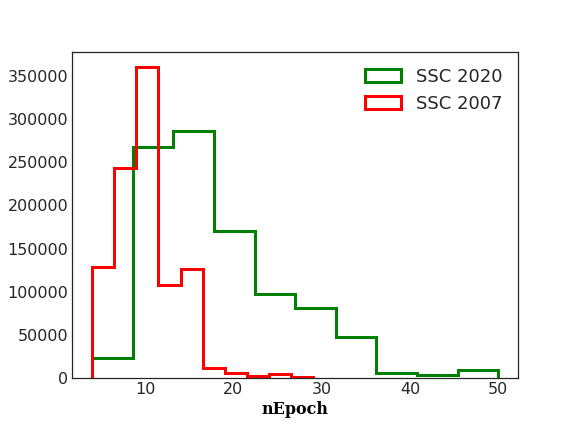
\includegraphics[width=0.4\textwidth, keepaspectratio]{figures/nepoch_compOvsN.png}
% 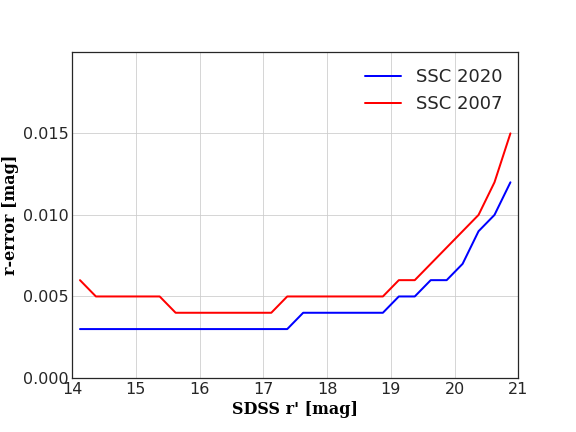
\includegraphics[width=0.4\textwidth, keepaspectratio]{figures/rerr_compOvsN.png}
% BW
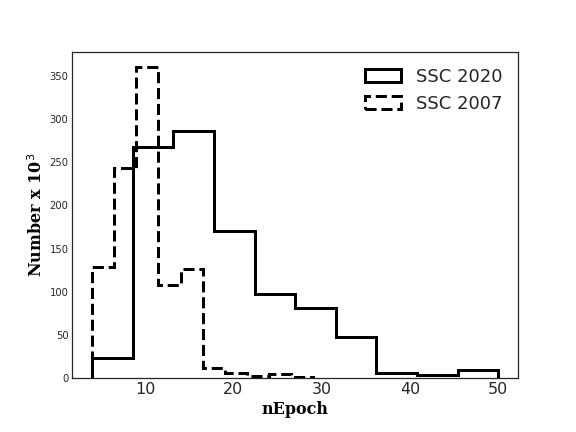
\includegraphics[width=0.4\textwidth, keepaspectratio]{figures/nepoch_compOvsN_BW.png}
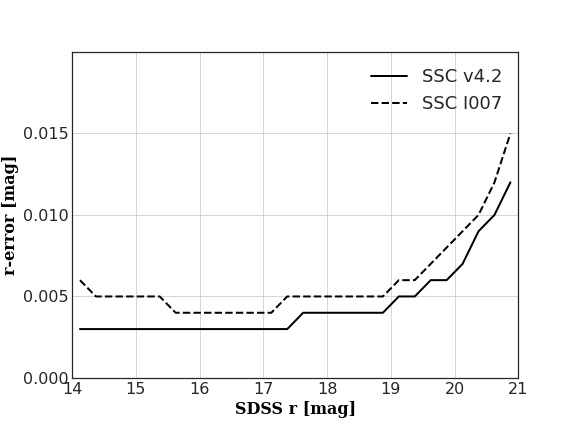
\includegraphics[width=0.4\textwidth, keepaspectratio]{figures/rerr_compOvsN_BW.png}
\caption{({\it Left}) A comparison of the number of observational epochs for matched stars in the 2020 versus 2007 Standard Star Catalog (SSC). ({\it Right}) A comparison of the median formal $r$ band photometric uncertainties of matched objects in the 2020 versus 2007 SSC, as a function of their mean $r$ magnitudes.
\label{fig:rerr_nvso}}
\end{figure*}

%%%%%%%%%%%%%%%%%%%%%%%%%%%%%%%%%%%%%%%%%

\subsection{The derivation of  photometric zeropoint corrections using Gaia EDR3 data\label{sec:GaiaCorr}} 

The variation of photometric zeropoints with position on the sky in the \pOc\ (see their eq.~4) was 
constrained using a combination of stellar colours \citep[the principal axes in colour-colour diagrams, for details 
see][]{2004AN....325..583I} and a standard star network \citep{2002AJ....123.2121S,2006AN....327..821T}. It is likely that 
residual errors in zeropoint calibration (e.g., a saw-tooth pattern as a function of Declination,
which was reported by \citealt{2013A&A...552A.124B}; see their Fig.~23) could be further minimized using 
uniformly calibrated space-based photometry from Gaia Early Data Release 3 (EDR3), as shown in this work. 

\subsubsection{Positional matching of the SDSS and Gaia catalogs}
Naively, one would positionally match the SDSS and Gaia EDR3 catalogs using a matching radius of 
about 0.3 arcsec because SDSS positions are accurate to better than 0.1 arcsec per coordinate (RMS) 
for sources with $r < 20.5$ mag \citep{2003AJ....125.1559P}.  However, observational epochs are
sufficiently different that stellar proper motions need to be accounted for; indeed, we find a very 
strong correlation between the SDSS-Gaia positional differences and proper motions published in 
the Gaia EDR3 catalog (see the left panel in  Figure~\ref{fig:GaiaRApm}). After accounting for proper
motions,  the positions agree at the level of $\sim28$ milliarcsec (robust\footnote{We use robust estimator 
of standard deviation computed as $\sigma_G = 0.741*(q_{75}-q_{25})$, where $q_{25}$ and $q_{75}$ are 
the 25\% and 75\% quantiles, and the normalization factor 0.741 assures that $\sigma_G$ is equal to 
standard deviation for normal (Gaussian) distribution.}
RMS, per coordinate). The 
residual differences are dominated by systematic errors in SDSS astrometry because there is
no increase of this RMS with magnitude (see the right panel in Figure~\ref{fig:GaiaRApm}), and
because the contribution of Gaia's astrometric measurement uncertainties is negligible. 
The implied SDSS astrometric accuracy of $\sim28$ milliarcsec is substantially better than 
the 0.1 arcsec reported by \cite{2003AJ....125.1559P}, but note that here we used 
positions ``averaged'' over typically $\sim20$ SDSS runs (see the left panel in Figure~\ref{fig:rerr_nvso}). 

\begin{figure*}
\centering 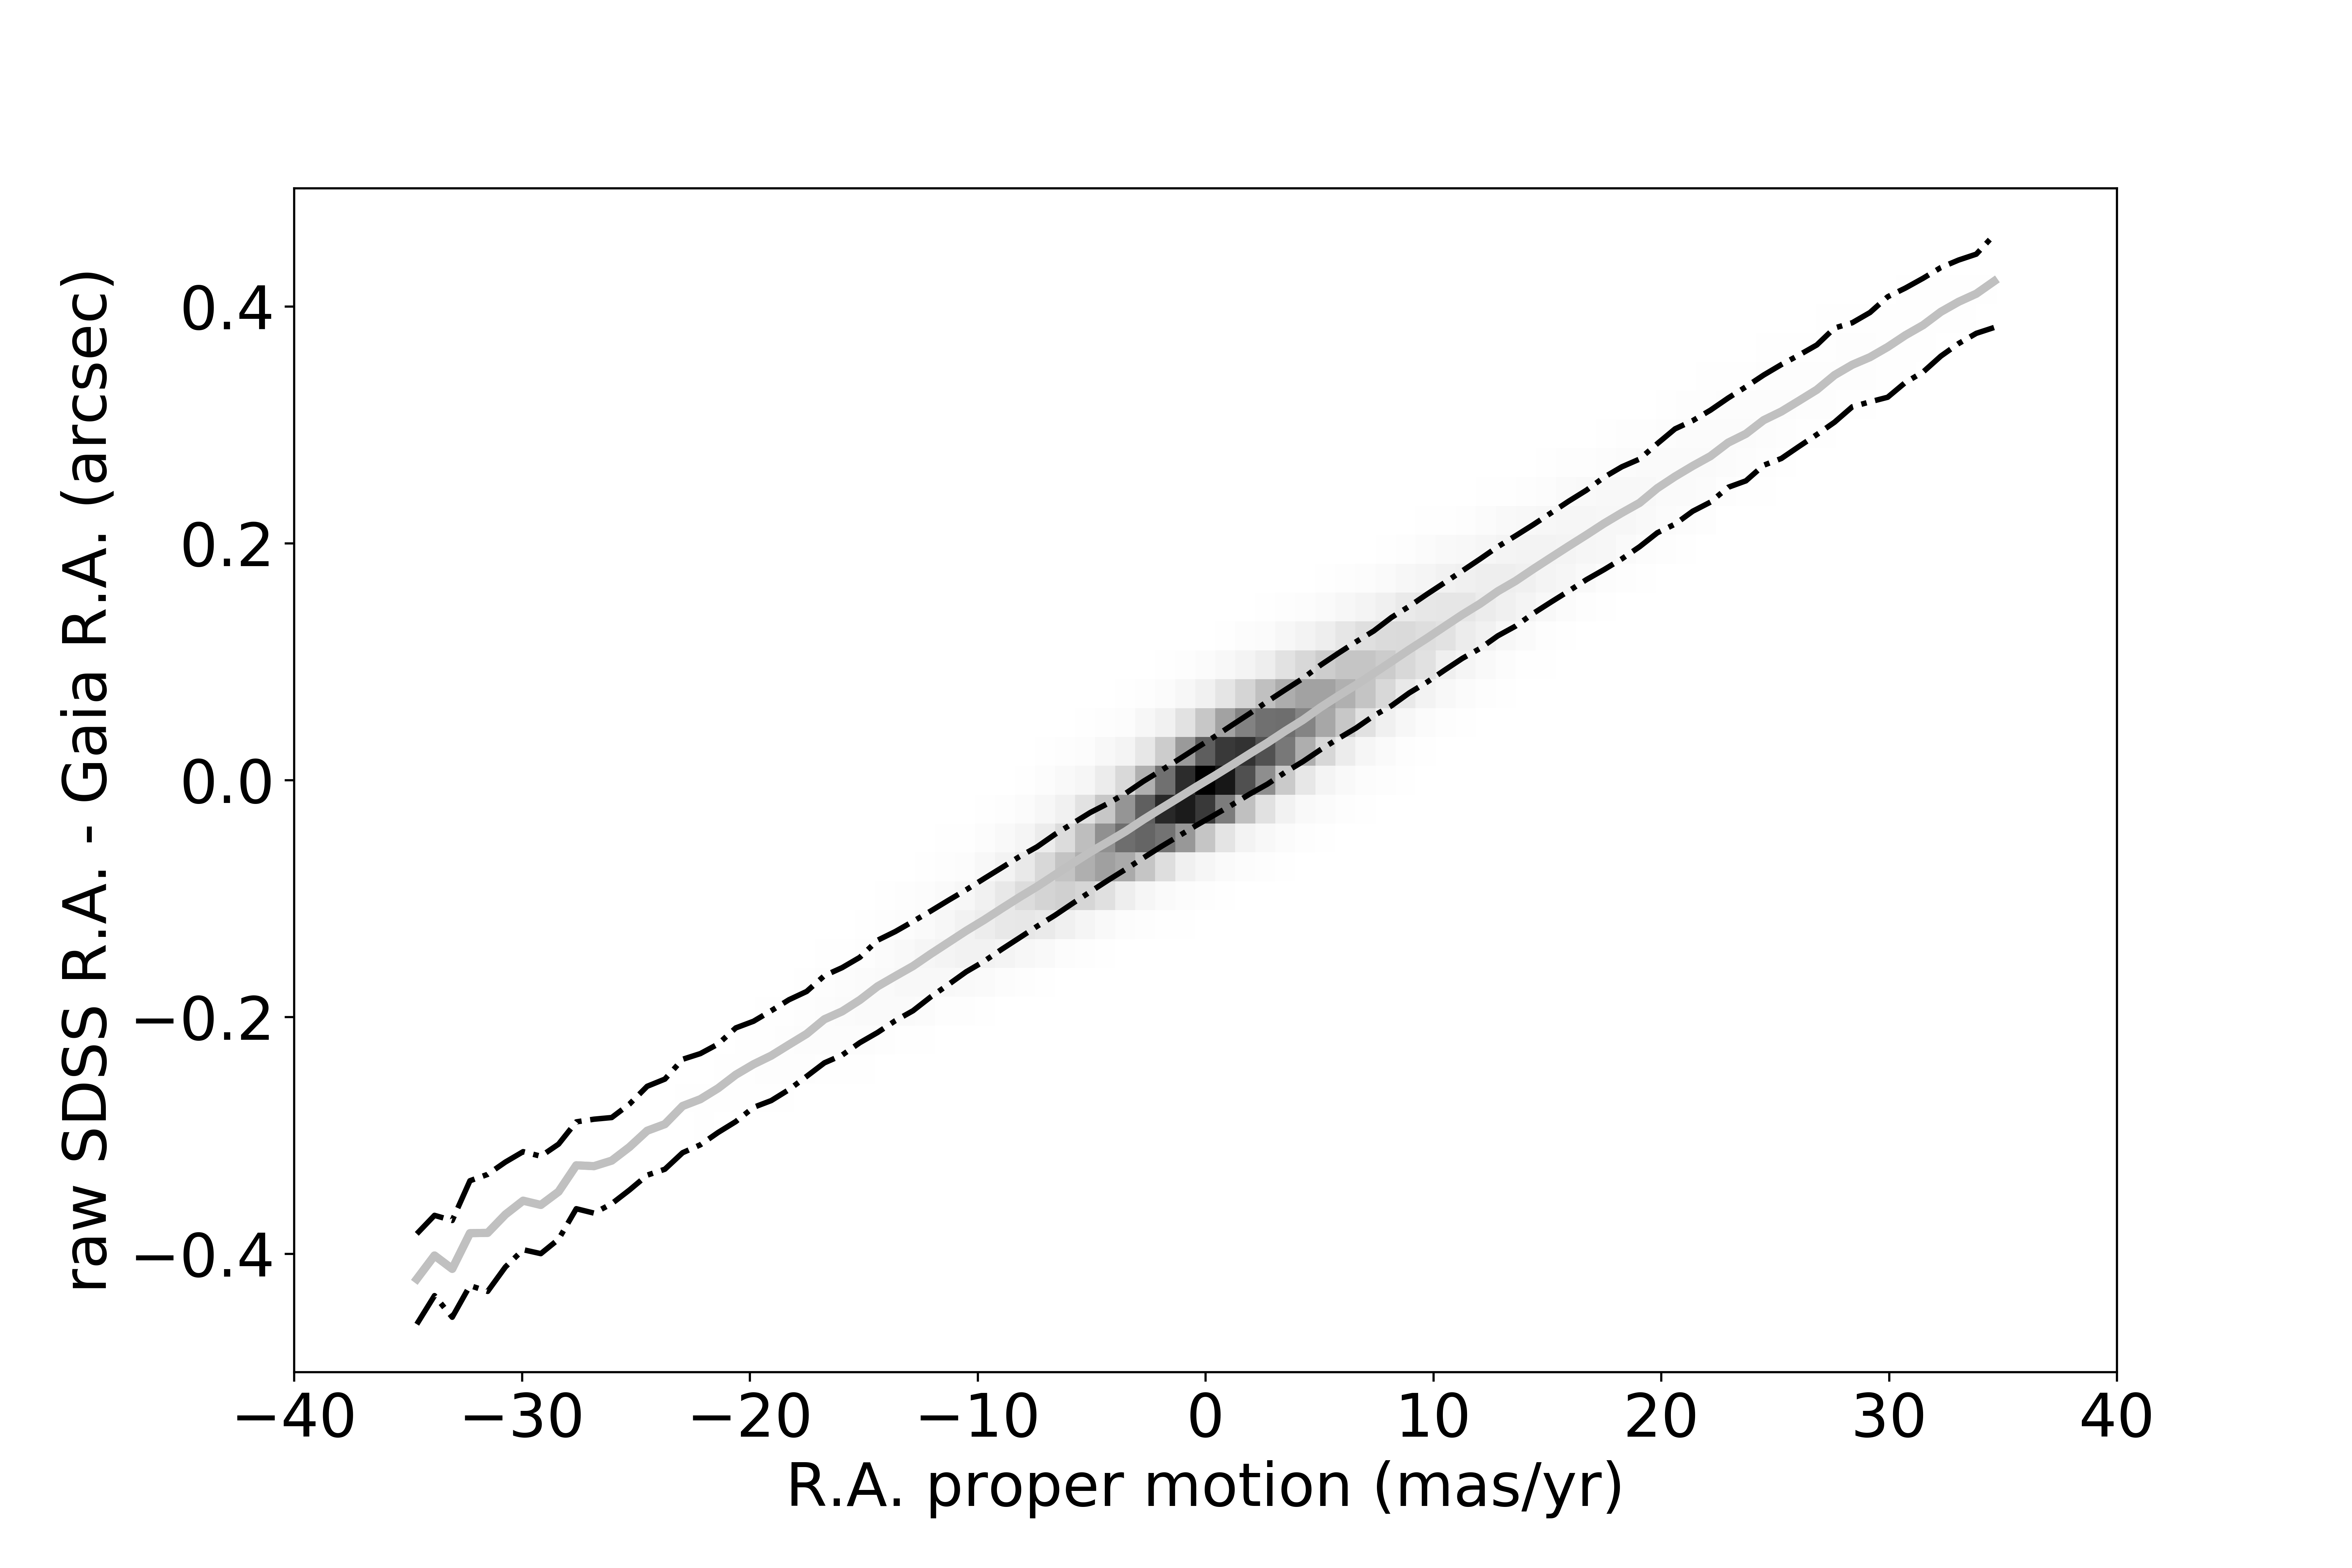
\includegraphics[width=0.4\textwidth, keepaspectratio]{figures/astroVSpm_RA_pm.png}
\centering 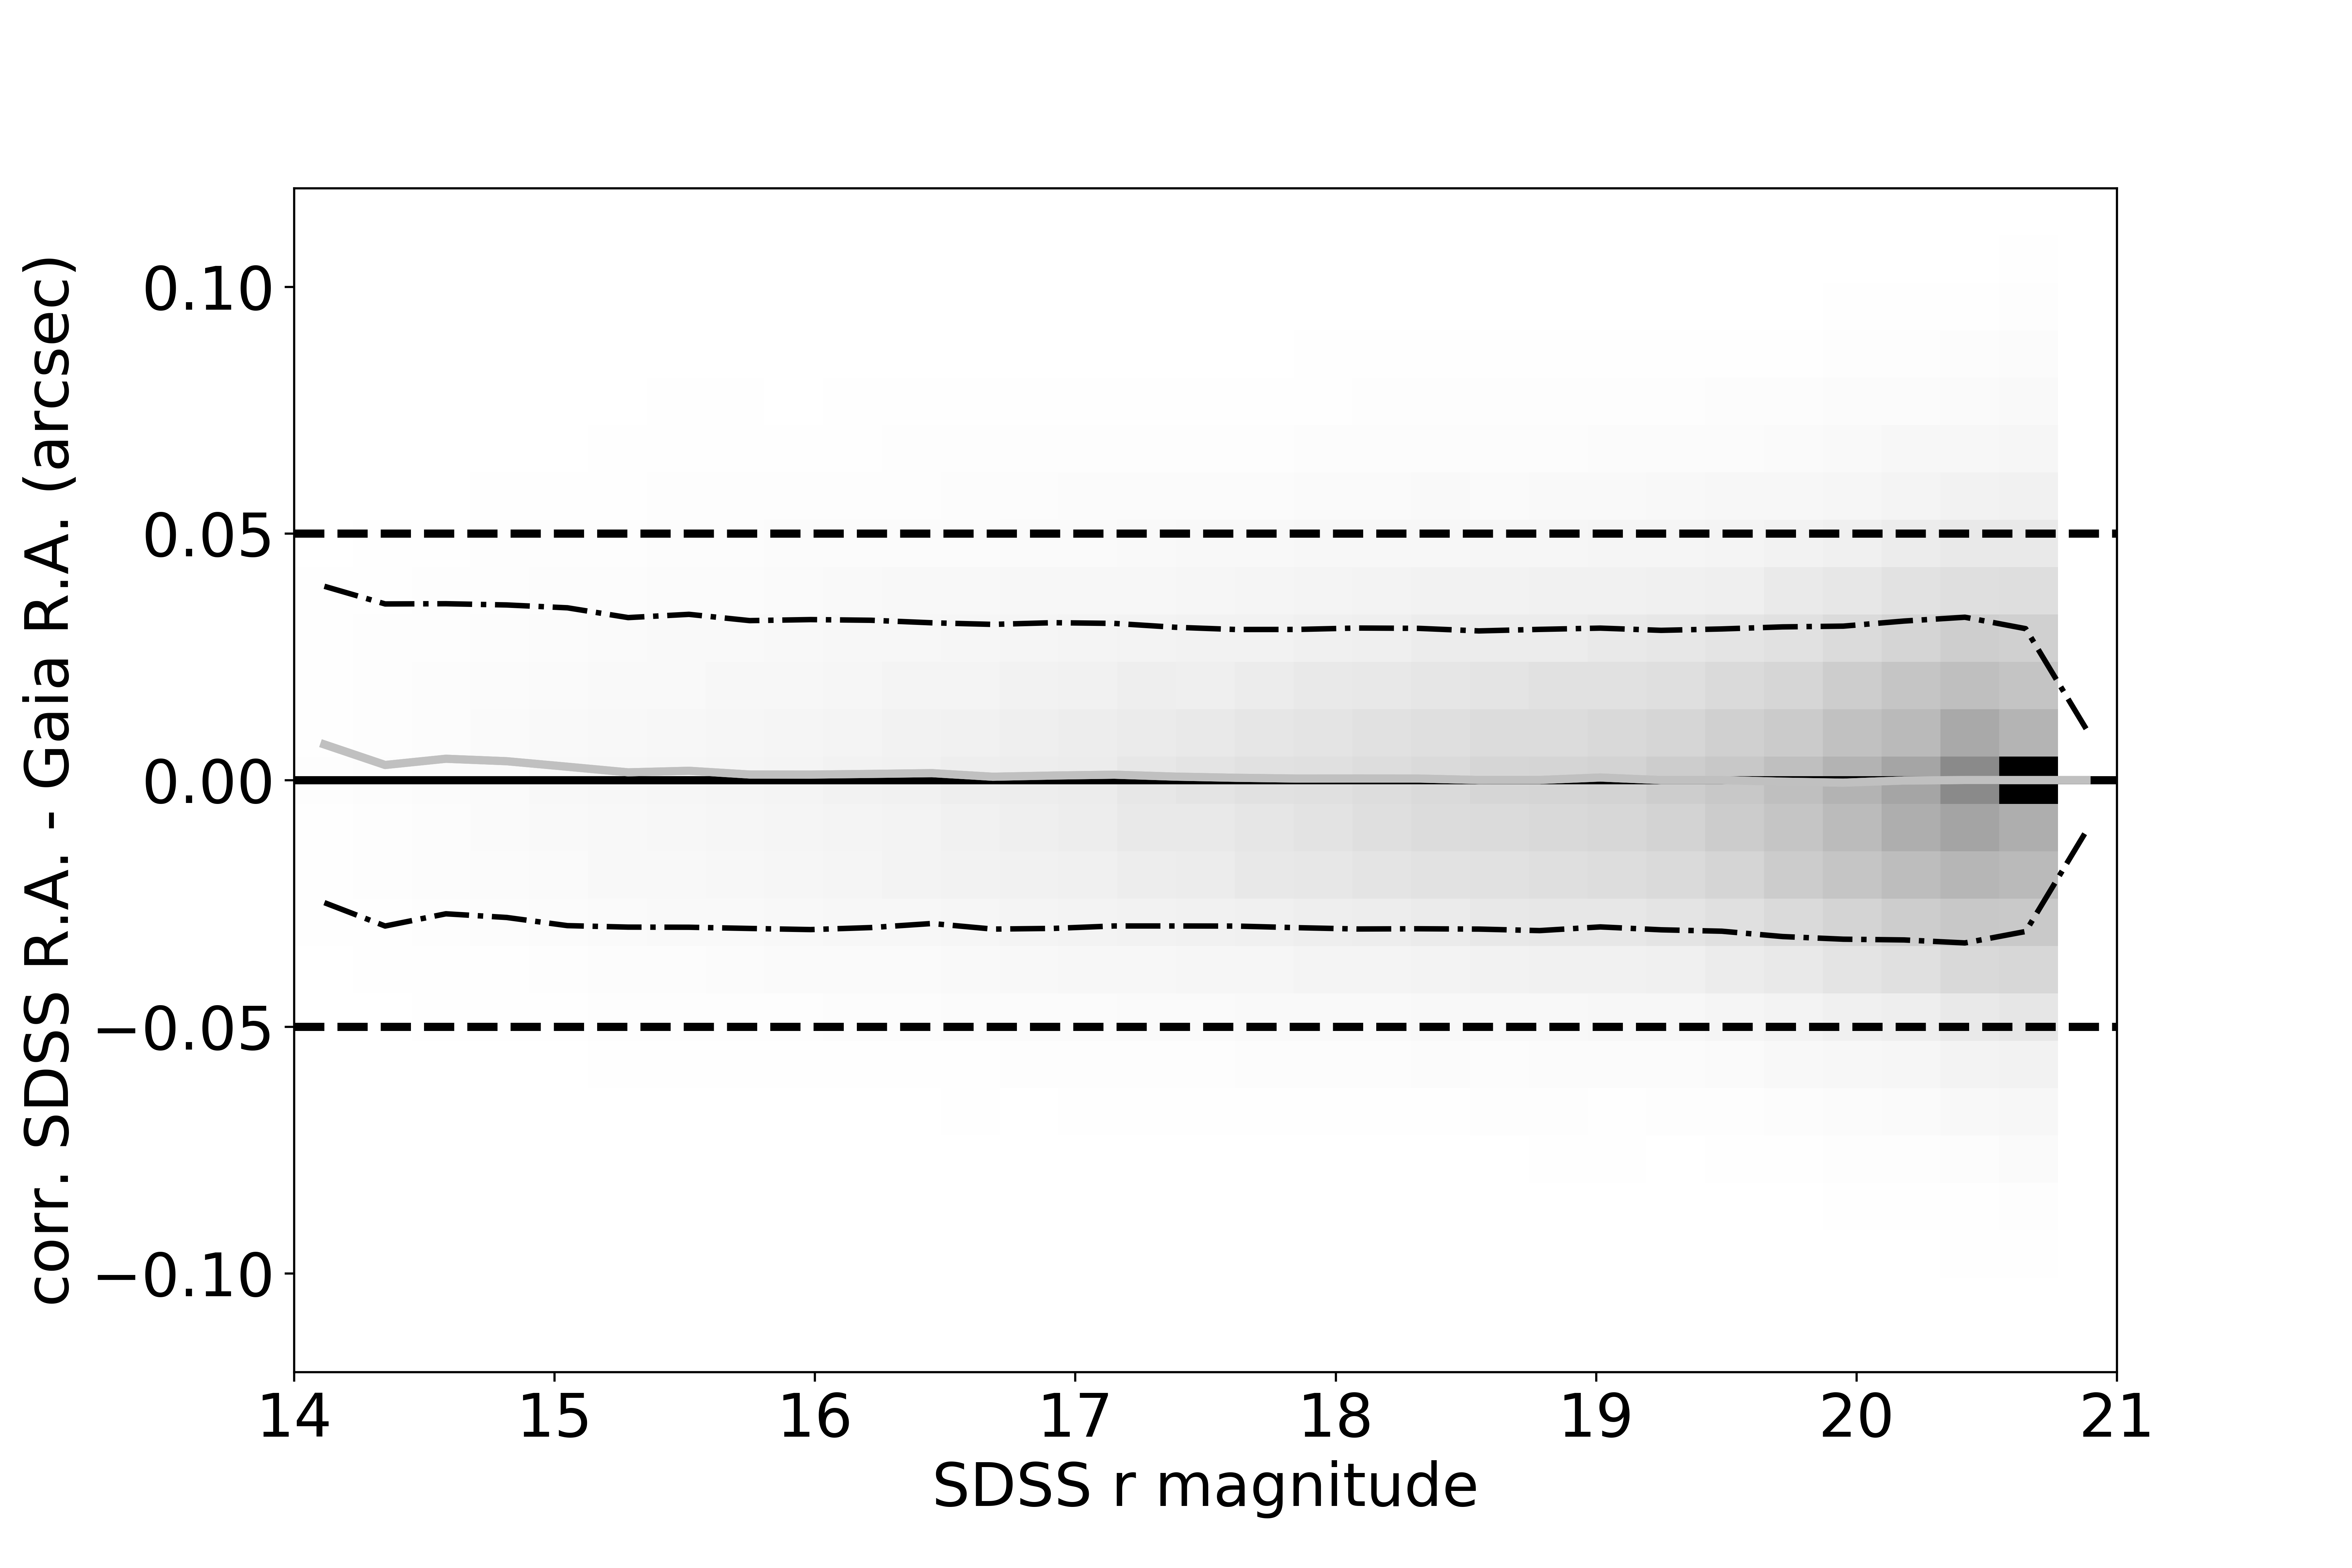
\includegraphics[width=0.4\textwidth, keepaspectratio]{figures/astroVSpm_RA_r.png}

\caption{({\it Left}) The R.A. difference between SDSS and Gaia 
vs. R.A. proper motion reported by Gaia EDR3. The solid line shows the median difference in bins 
of proper motion and the dashed lines mark the $\pm \sigma_G$ envelope around the medians,
where $\sigma_G$ is the robust standard deviation. ({\it Right}) The R.A. difference 
after correcting using the best-fit R.A. difference vs. 
proper motion curve, as a function of the SDSS $r$ magnitude. The residual differences are dominated 
by systematic errors in SDSS astrometry at the level of $\sim28$ milliarcsec (note that there is no increase with 
magnitude). Analogous plots for Declination quantities are similar. 
\label{fig:GaiaRApm}}
\end{figure*}

%%%%%%%%%%%%%%%%%%%%%%%%%%%%%%%%%%%%%%%%%

\subsubsection{Gaia-based photometric zeropoint corrections  \label{sec:GaiaCorr2}}

Gaia EDR3 reported Gmag magnitudes, which approximately span the SDSS $griz$ bandpasses, 
and BP and RP magnitudes, which approximately correspond to the blue and red halves of the 
Gmag bandpass. We first used Gmag data to derive ``gray'' zeropoint corrections (applied to
all five SDSS bands), and then use the BP-RP colour to derive zeropoint corrections for the 
$ugiz$ bands, relative to the $r$ band. 

The basic idea is simple: use Gaia's Gmag, Gmag$_{GaiaEDR3}$, and the SDSS $gri$ magnitudes
to derive synthetic Gmag magnitudes based on SDSS data, Gmag$_{SDSS}$; bin the 
$\Delta$Gmag = (Gmag$_{SDSS}$-Gmag$_{GaiaEDR3}$) residuals by R.A. and Dec, and 
use the median residuals per bin as the gray correction for SDSS photometry (as functions
of R.A. and Dec). Similarly, use Gaia's BP-RP colour to derive synthetic $u-r$, $g-r$, $r-i$
and $r-z$ colours, and use the median residuals per bin as zeropoint corrections for 
the $ugiz$ bands. 

Given a large number of matched stars ($\sim 400,000$), and a large number of colour combinations,
we do not attempt to derive analytic fits for synthetic magnitudes and colours but instead
use 0.05 mag narrow colour bins and linear interpolation between the bins. We have verified
that even sixth-order polynomial fits do not provide better results than this simple 
numerical approach. An example of such a transformation is shown in Figure~\ref{fig:GrVSgi}. 


\begin{figure}
  \centering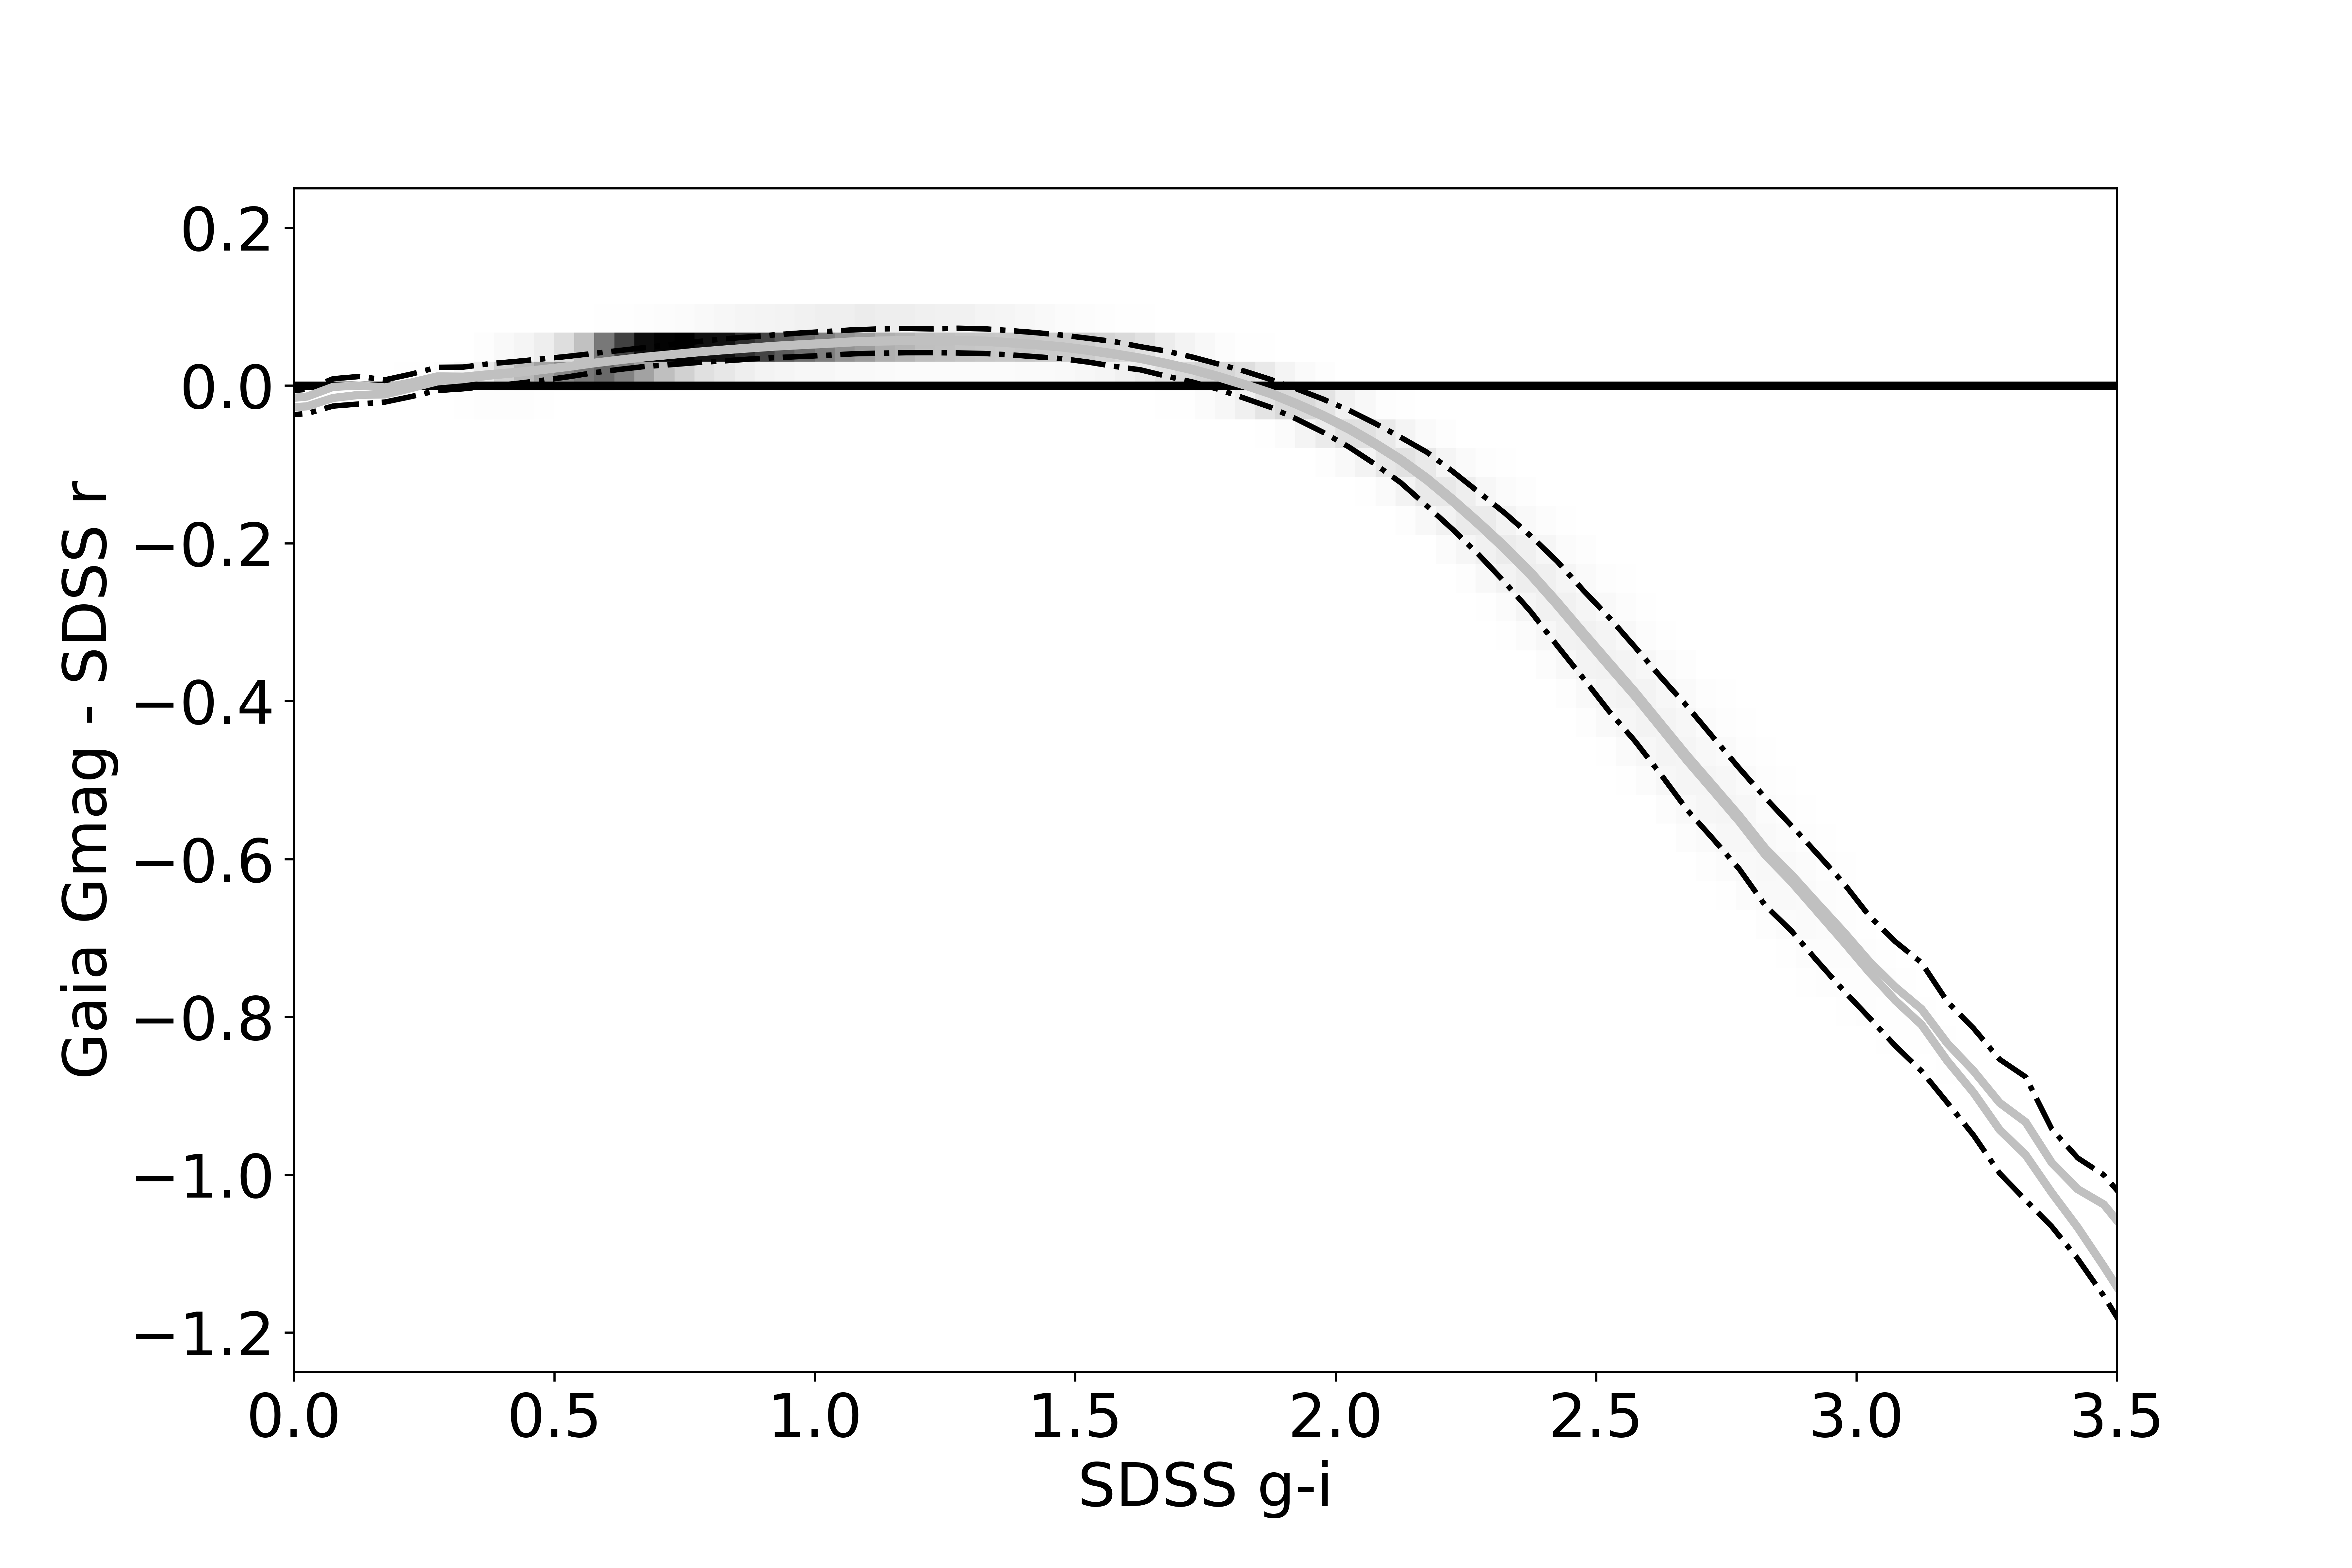
\includegraphics[width=0.95\columnwidth]{figures/GrVSgi.png} 
\caption{The variation of the difference between Gaia's Gmag magnitude from Early Data Release 3
and SDSS $r$ magnitude with the SDSS $g-i$ colour.
The  colour map illustrates the distribution of $\sim 393,000$ matched stars with 
$16<$Gmag$<19.5$. The two (barely distinguishable) solid lines represent the median 
values $\pm$ uncertainty of the median for 0.05 mag wide $g-i$ bins. The short-dashed 
lines show the median values $\pm$ the robust standard deviation for 
each bin. The horizontal solid line at zero is added to guide the eye. The mean of 
the two solid lines is used to derive the gray zeropoint correction, as a function of R.A.
and Declination.}
\label{fig:GrVSgi}
\end{figure}


The variation of Gmag residuals with Gmag (see Figure~\ref{fig:gaiaJump}) shows 
an overall gradient of $\sim10$ millimag from bright (G=16) to faint (G=20) end. 
A comparison of the SDSS catalog with Pan-STARRS and DES catalogs (see 
Section~\ref{sec:DESPS1} and Figure~\ref{fig:drVSr}) strongly suggests that the
origin of this discrepancy is a magnitude-dependent bias in Gaia's Gmag photometry,
rather than a problem with the SDSS catalog (offsets between the SDSS and DES
photometry,  are $<2$ millimag at Gmag$\sim$20, and $<5$ millimag when
comparing to Pan-STARRS). 


\begin{figure}
    \centering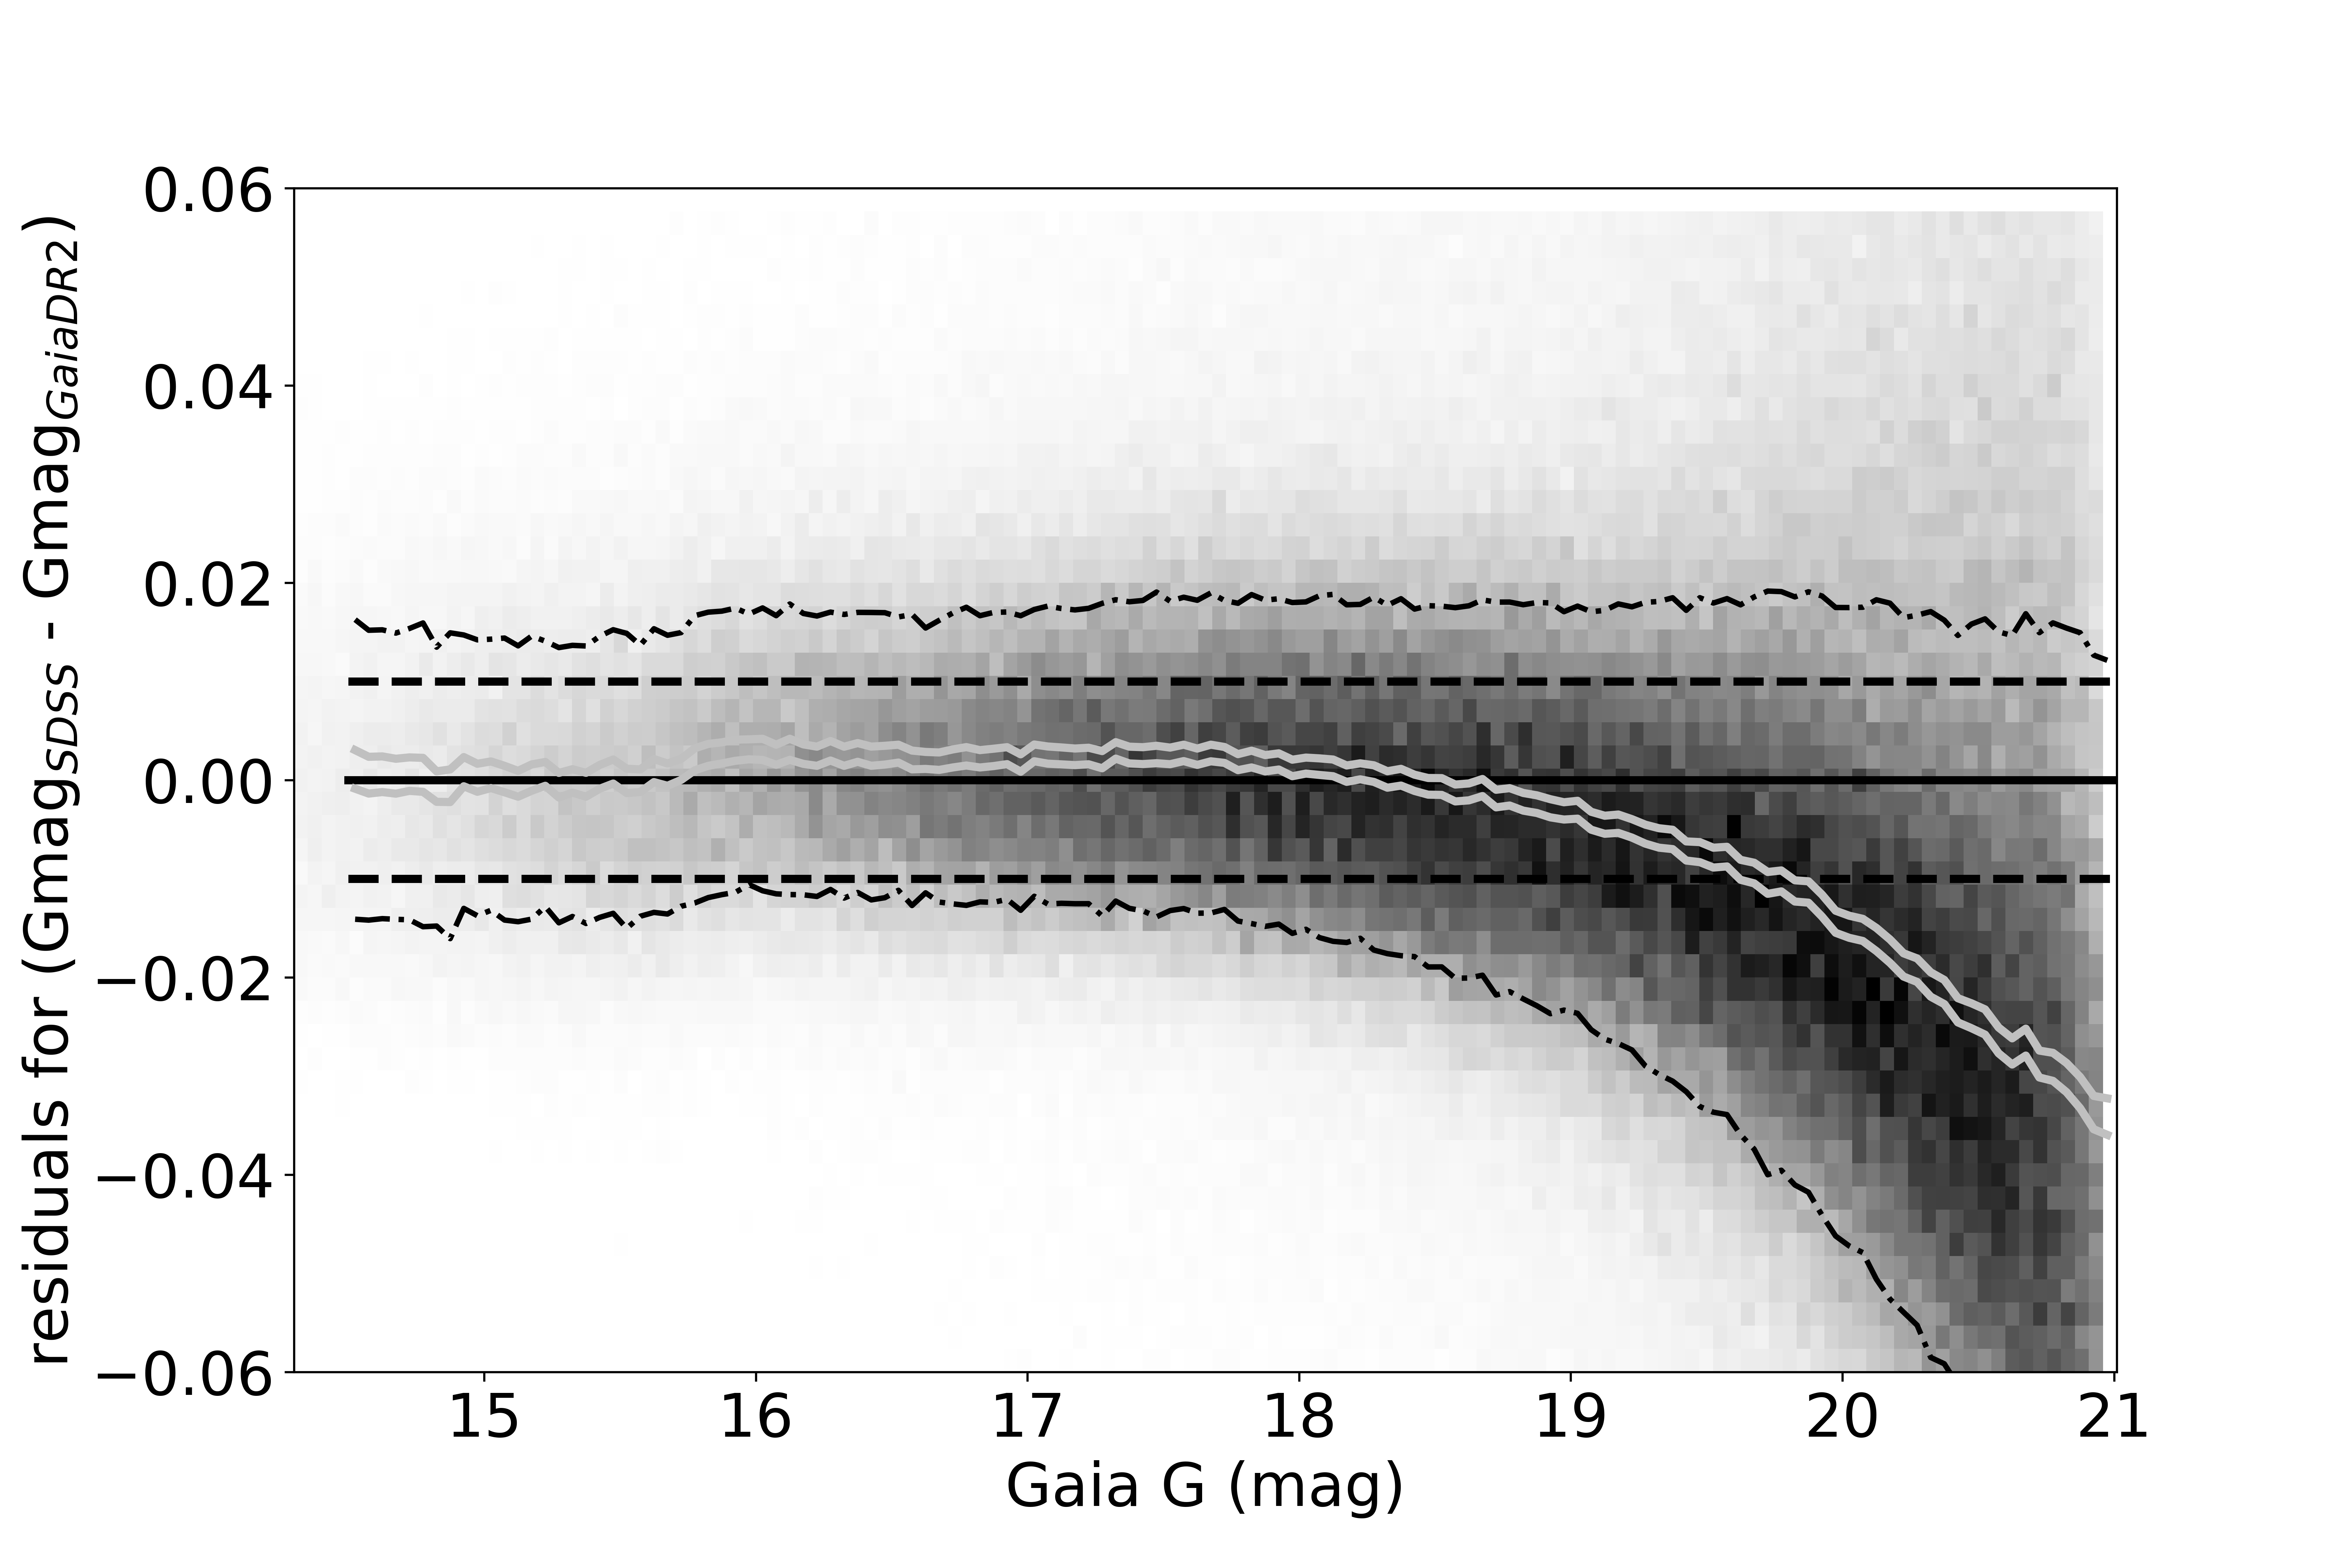
\includegraphics[width=0.95\columnwidth]{figures/GmagCorrectionTest_Gmag_Hess.png} 
\caption{The variation of the residuals between Gaia's Gmag from Early Data Release 3
and synthetic Gmag values generated using SDSS $gri$ photometry. The two solid 
lines represent the median values $\pm$ uncertainty of the median for each
0.05 mag wide Gmag bin. The short-dashed lines show the median values $\pm$ 
the robust standard deviation for each bin. The horizontal solid and long-dashed 
lines at zero and $\pm$0.01 mag, respectively, are added to guide the eye.
Note an overall gradient of $\sim0.01$ mag from bright (G=16) to faint (G=20) 
end -- a comparison of the SDSS catalog with Pan-STARRS and DES catalogs (see 
Figure~\ref{fig:drVSr}) suggests that its origin is a magnitude-dependent bias in
 Gaia's EDR3 photometry rather than a problem with SDSS photometry.}
\label{fig:gaiaJump}
\end{figure}


Given these two features, we limit the calibration sample to the $16<$Gmag$<19.5$
magnitude range. We further restrict calibration stars to the $0.4 < g-i < 3.0$ colour 
range (approximately A0 to M5 spectral range), yielding a sample of $\sim372,000$ stars. 
The behavior of median Gmag residuals per R.A. and Declination bin are shown in 
the left and right panels respectively of Figure~\ref{fig:graycorrRA}.% and \ref{fig:graycorrDec}. 


\begin{figure*}
  \centering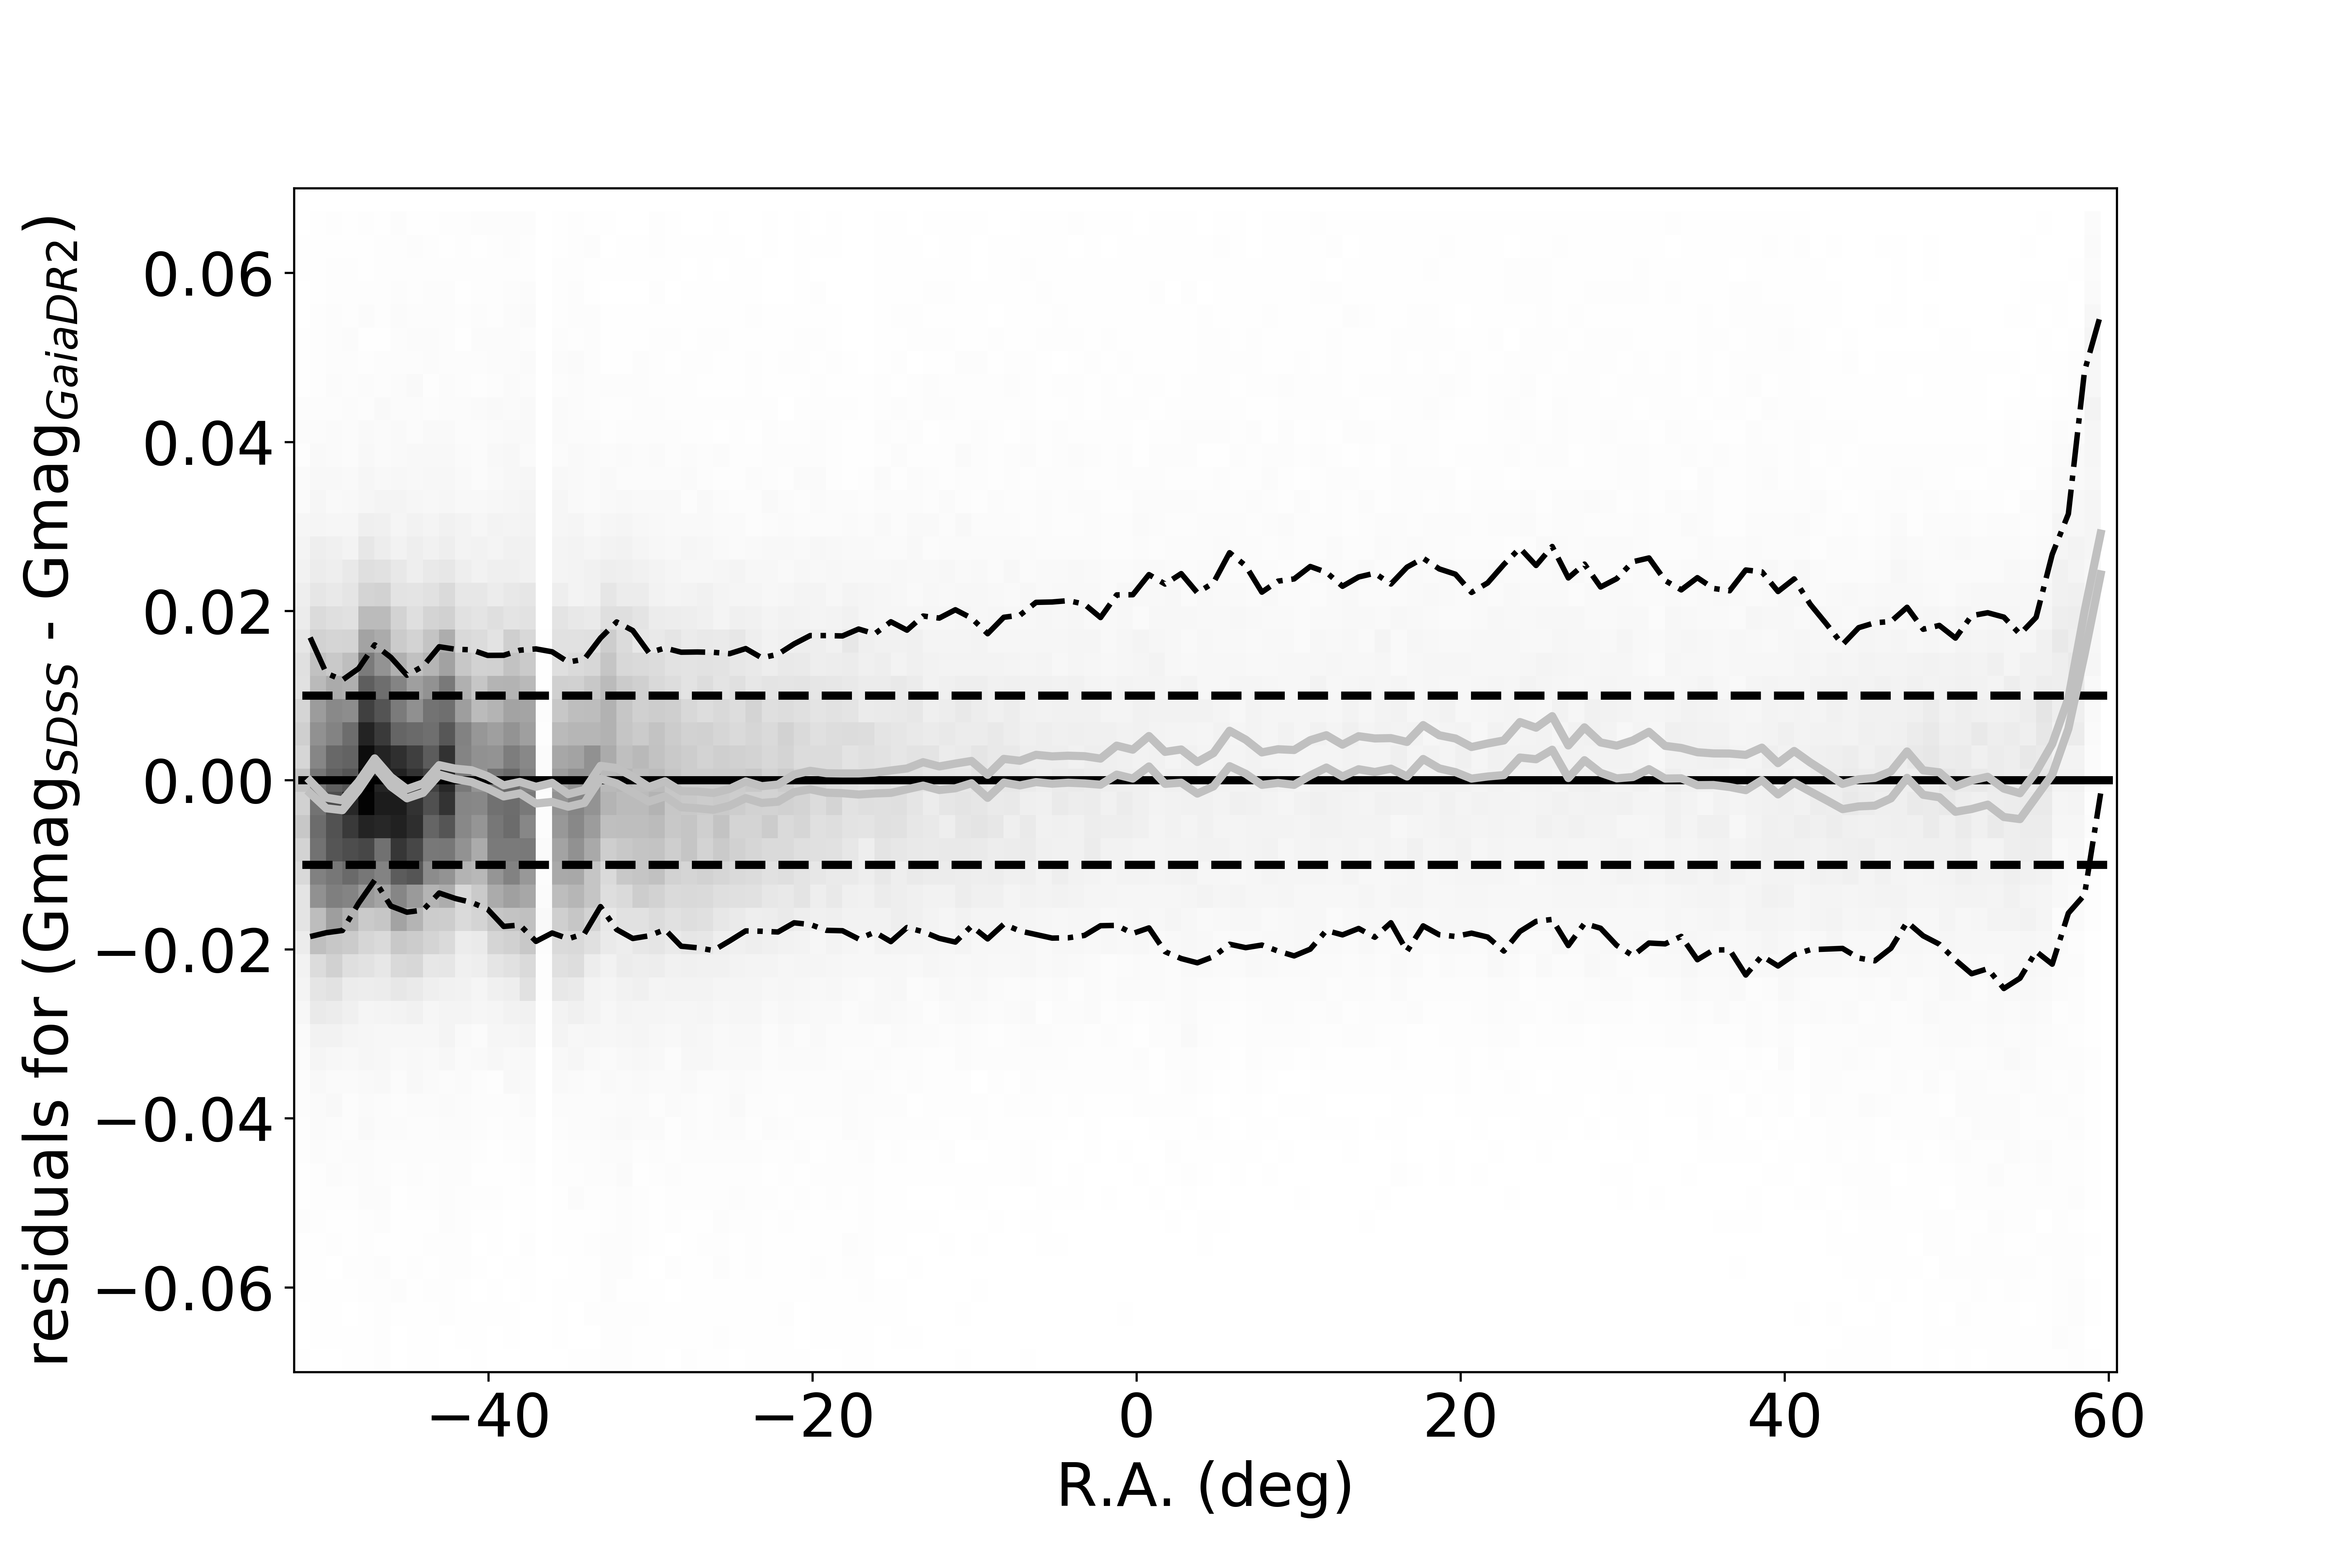
\includegraphics[width=0.45\textwidth]{figures/GmagCorrection_RA_Hess.png} 
  \centering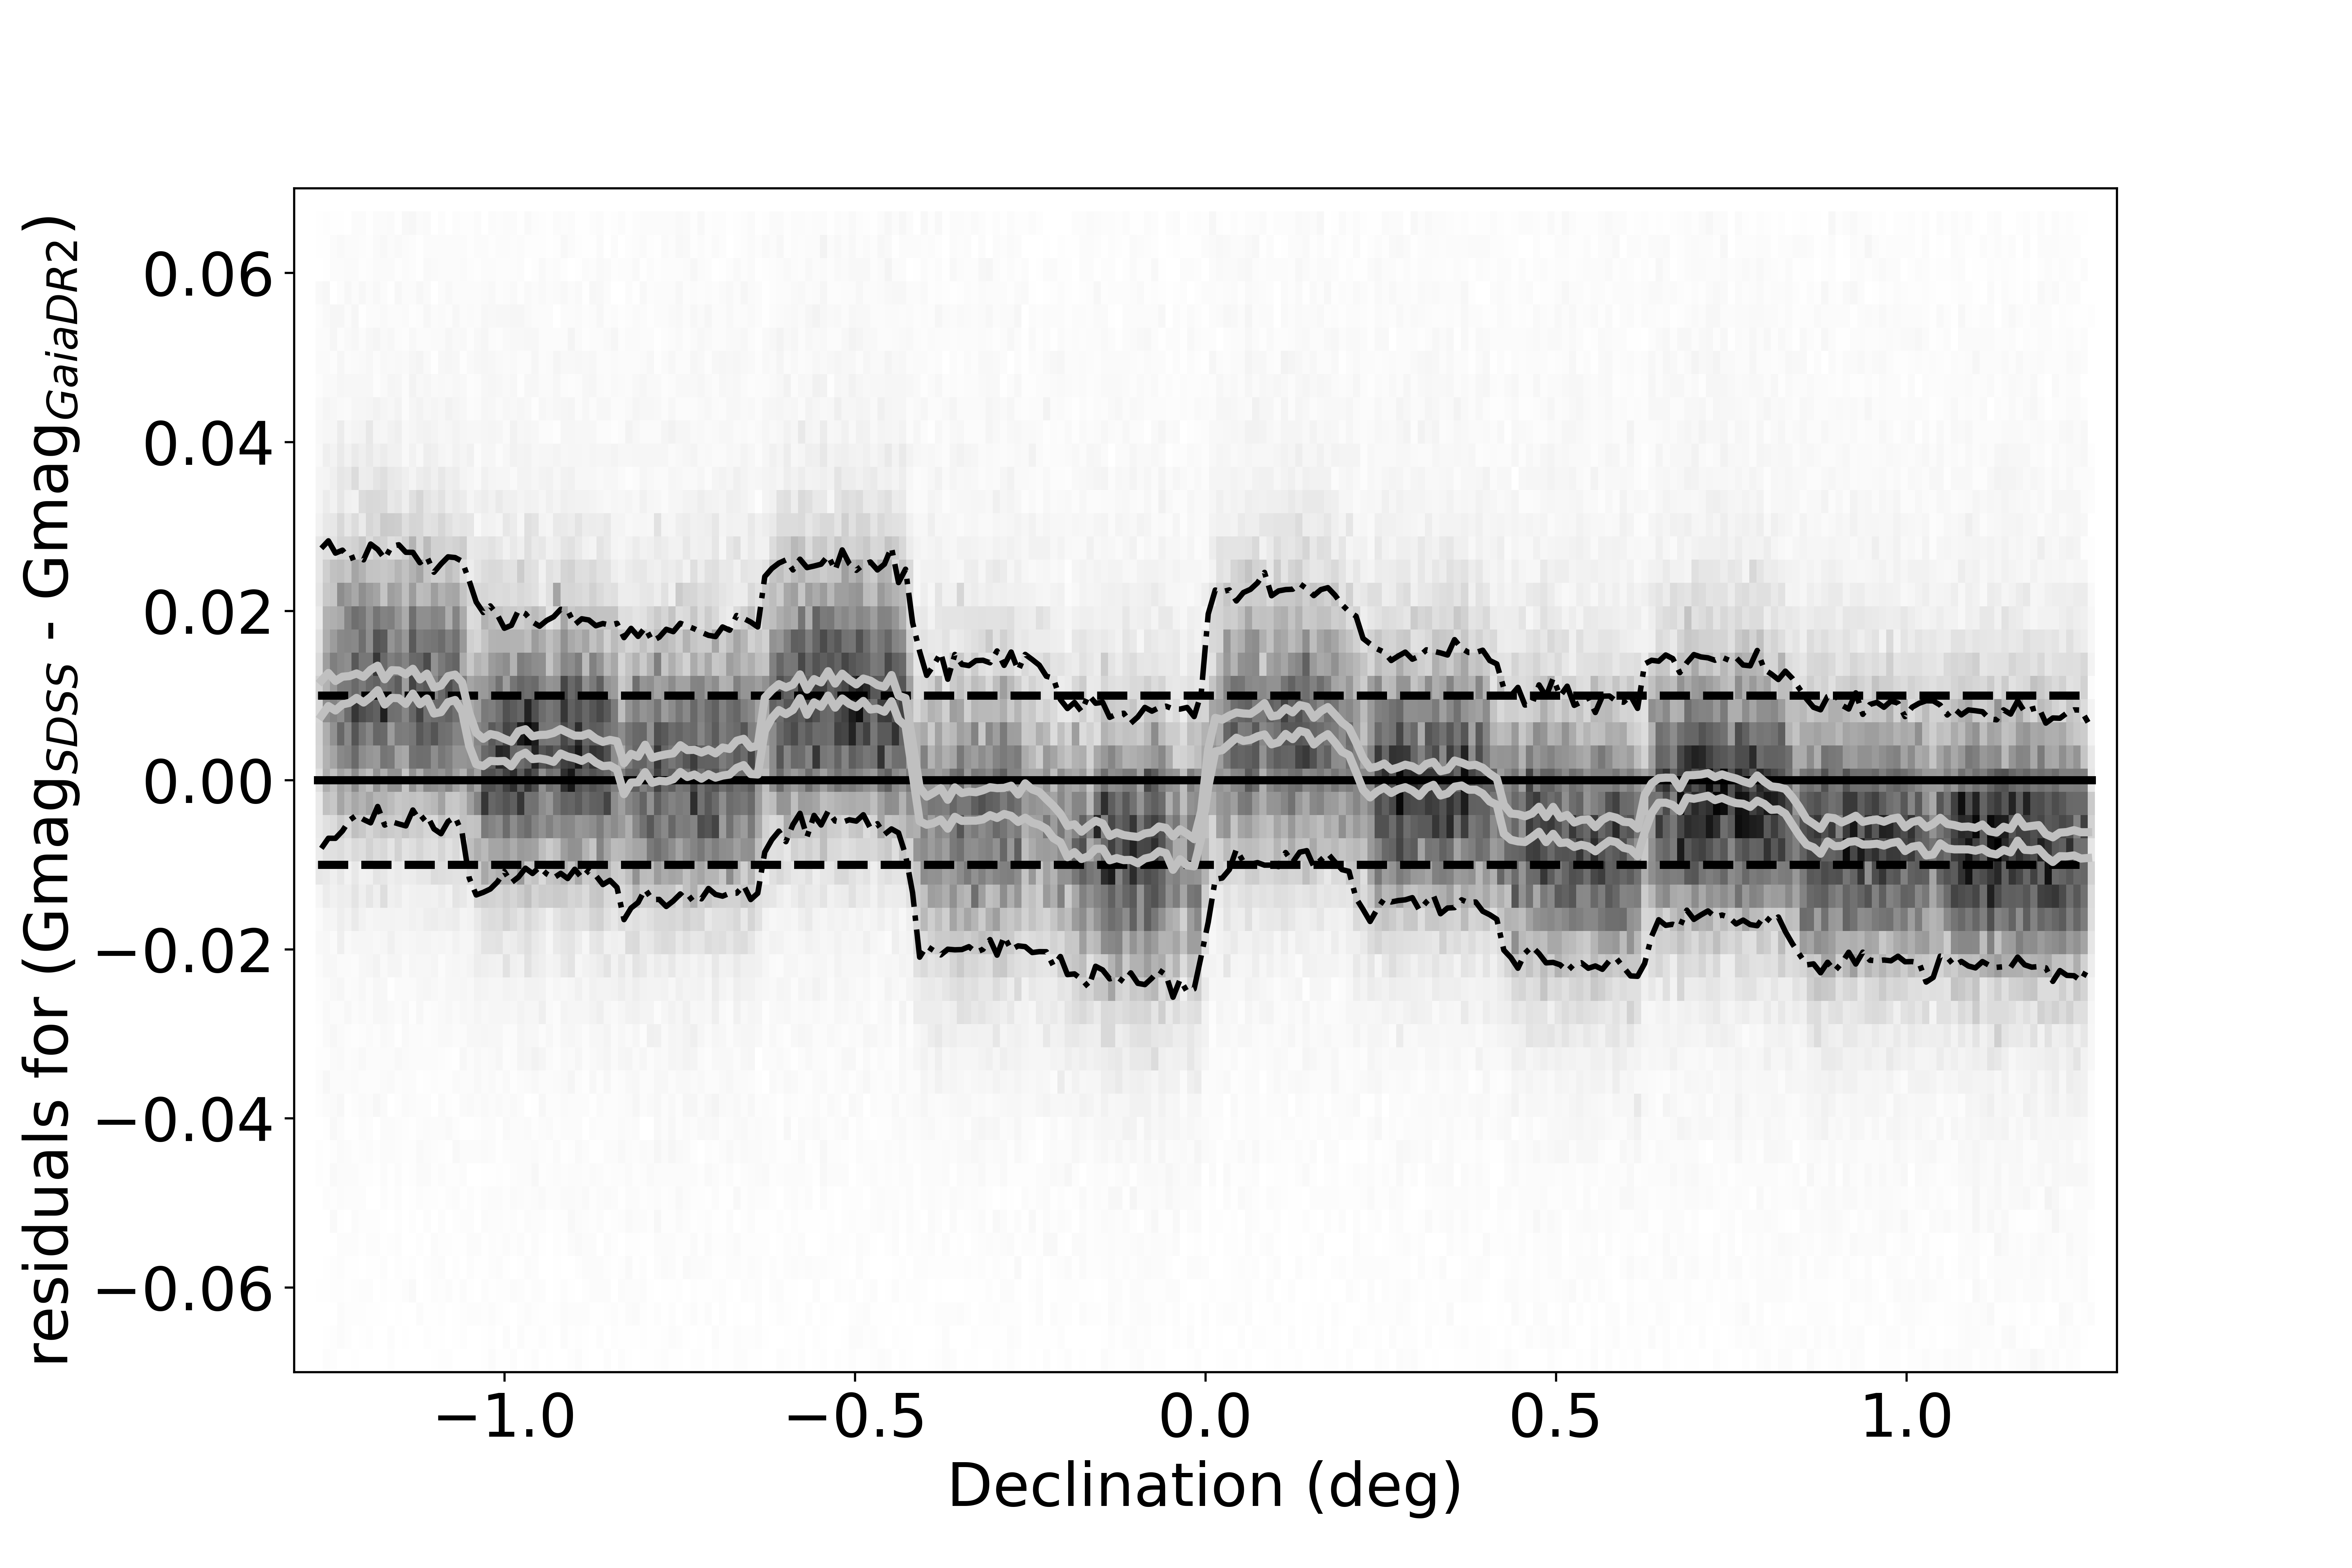
\includegraphics[width=0.45\textwidth]{figures/GmagCorrection_Dec_Hess.png} 
\caption{({\it Left}) The R.A. variation of the residuals between Gaia's Gmag from EDR3
and synthetic Gmag values generated using SDSS $gri$ photometry. The 
colour map illustrates the distribution of $\sim 372,000$ matched stars with 
$16<$Gmag$<19.5$ and $0.4 < g-i < 3.0$. The two solid lines represent the 
median values $\pm$ uncertainty of the median for 1 degree wide R.A. bins. 
The short-dashed lines show the median values $\pm$ the robust standard 
deviation for each bin. The horizontal solid and long-dashed lines at zero and 
$\pm$0.01 mag, respectively, are added to guide the eye. The mean of the two 
solid lines is the gray correction, as a function of R.A., applied to the SDSS 
$ugriz$ magnitudes. The standard deviation for the applied correction is 3.2 millimag. {\it Note}: The stripe of missing data seen at R.A.$\sim$ -37 deg is due to the presence of the globular cluster, $M2$. The resulting high stellar density region was masked off during data processing.
({\it Right}) Analogous to the left panel, except that here results are shown for
0.01 degree wide Declination bins. The 12 clearly visible regions correspond to
two SDSS scans (in R.A. direction) and six CCD columns in the SDSS camera. 
The standard deviation for the applied correction is 6.5 millimag, with a maximum
absolute value of $\sim0.01$ mag.}
\label{fig:graycorrRA}
\end{figure*}

% \begin{figure}
%     \centering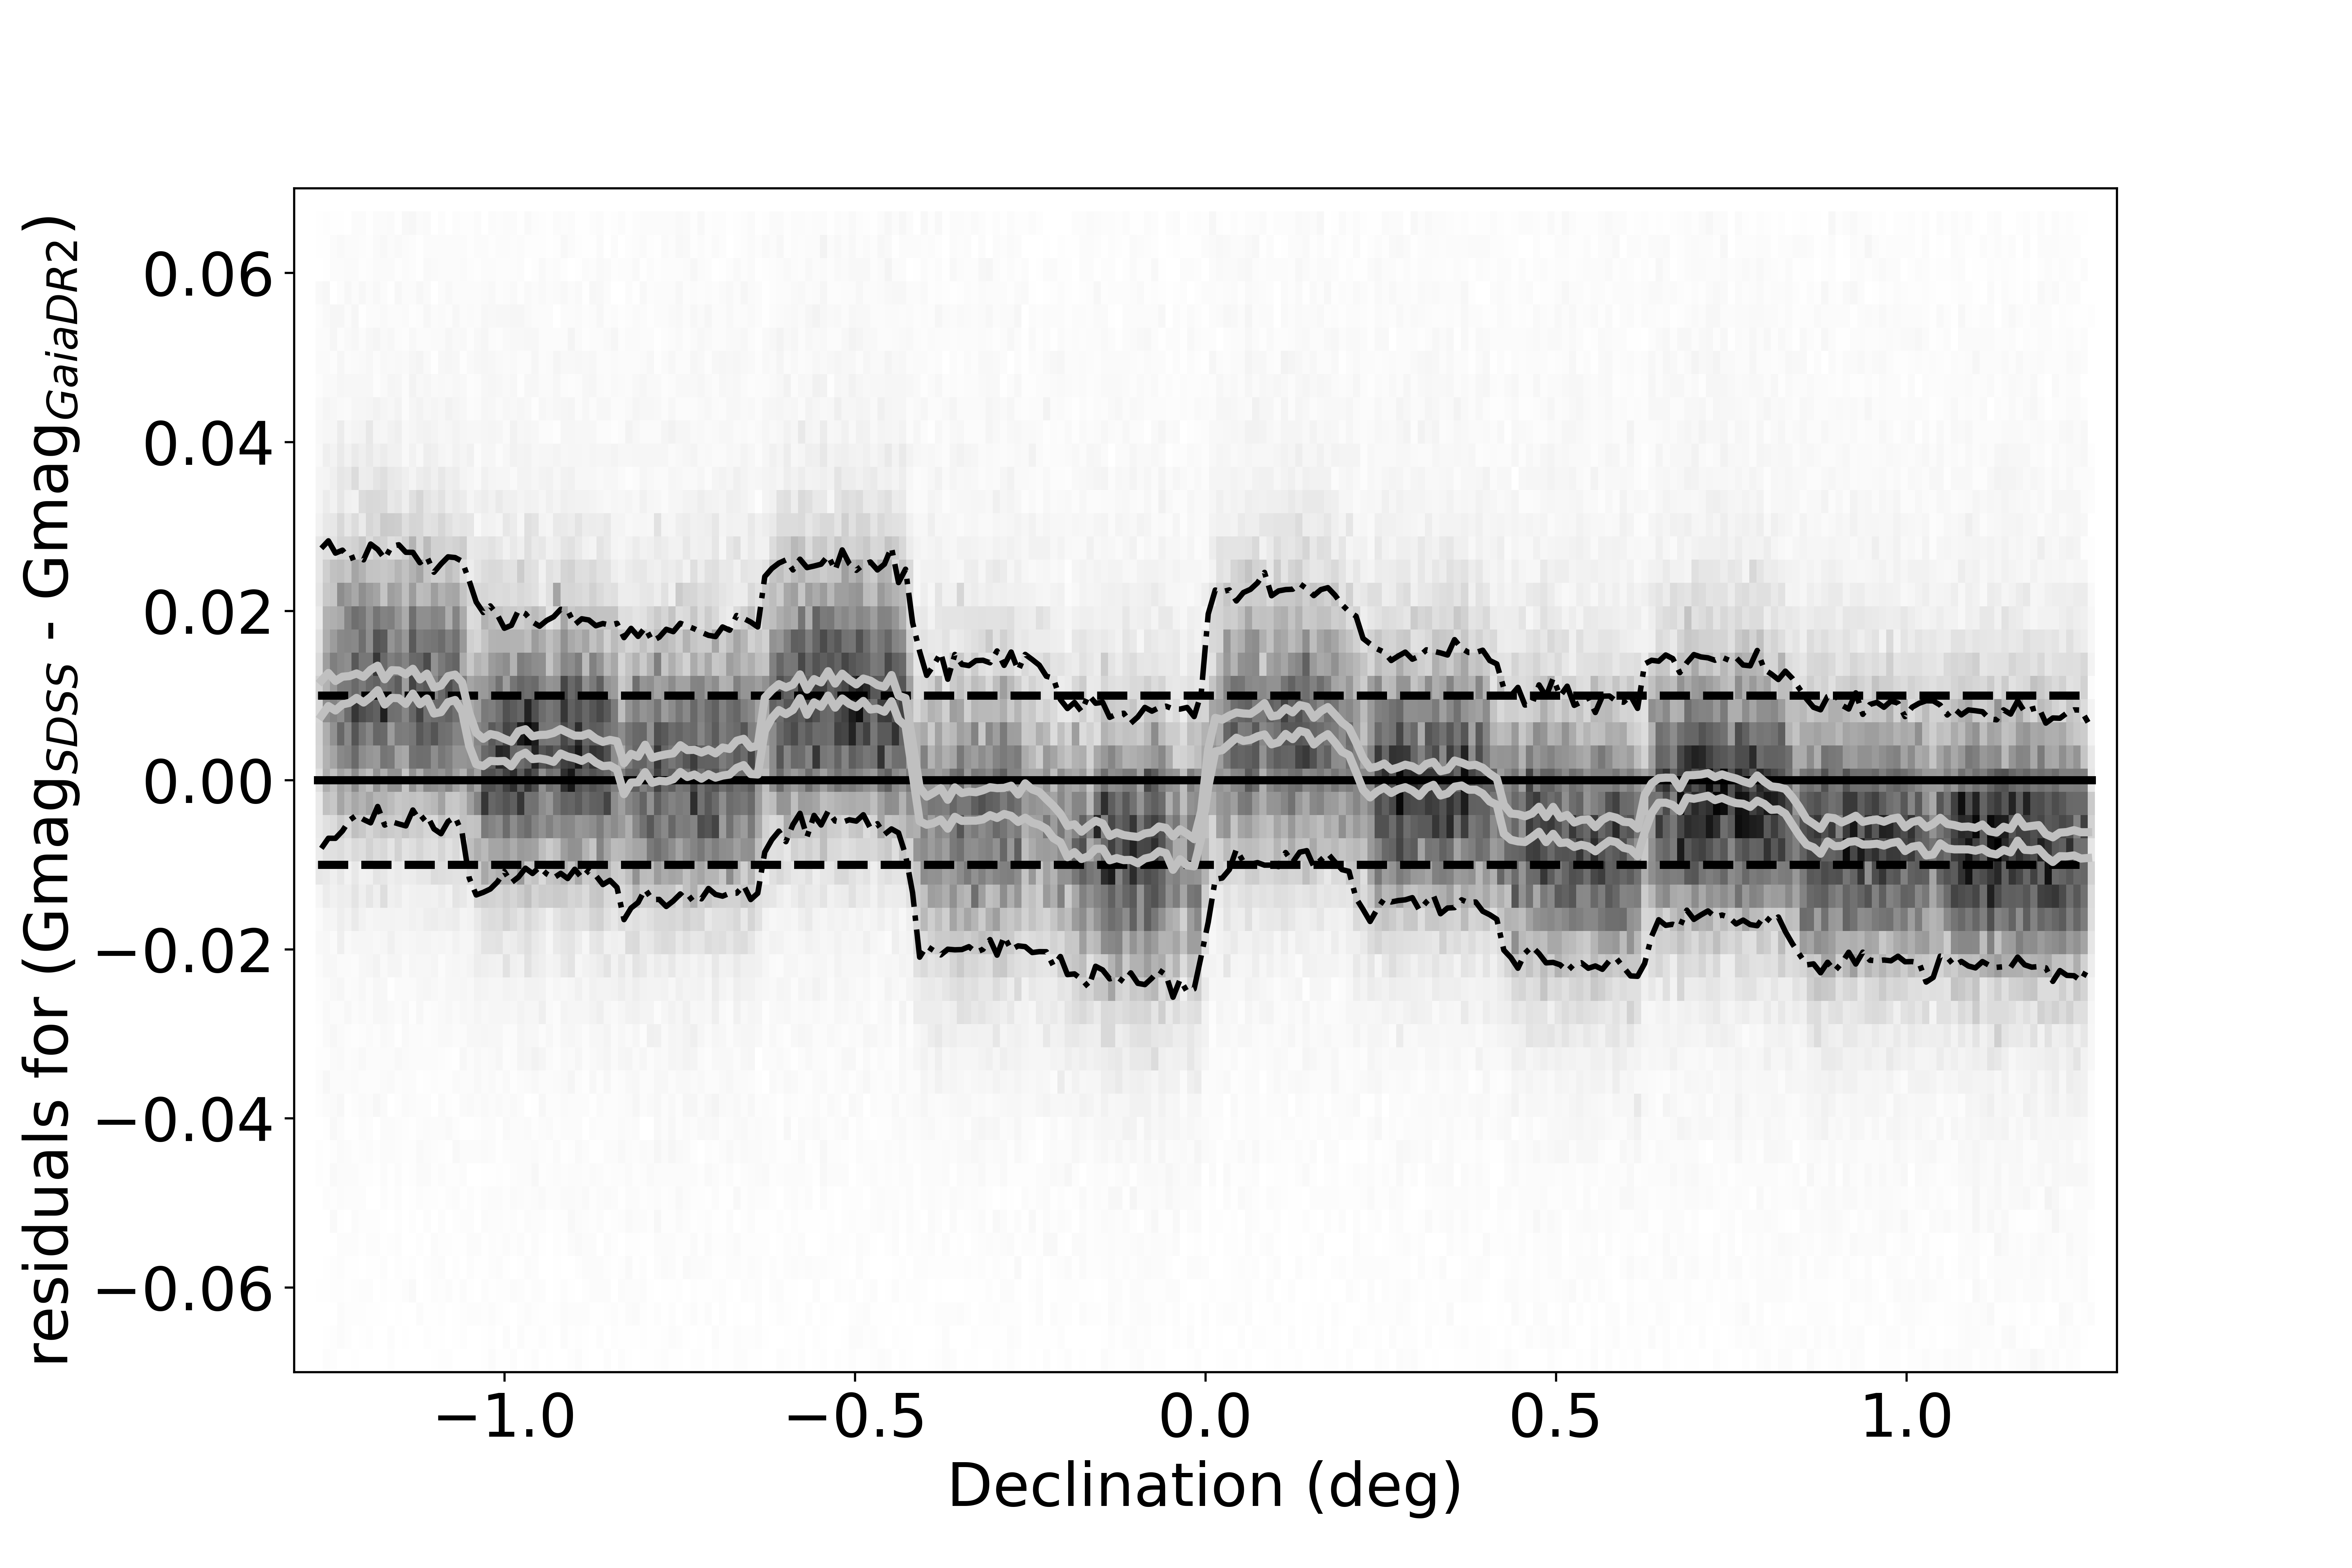
\includegraphics[width=0.95\columnwidth]{figures/GmagCorrection_Dec_Hess.png} 
% \caption{Analogous to Figure~\ref{fig:graycorrRA}, except that here results are shown for
% 0.01 degree wide Declination bins. The 12 clearly visible regions correspond to
% two SDSS scans (in R.A. direction) and six CCD columns in the SDSS camera. 
% The standard deviation for the applied correction is 6.5 millimag, with a maximum
% absolute value of $\sim0.01$ mag.}
% \label{fig:graycorrDec}
% \end{figure}


\tbd{Except for a few degrees long region at the edge of Stripe 82 (R.A.$>$55 deg), the
SDSS photometric zeropoints are remarkably stable with respect to R.A.}; the scatter
is only 3.5 millimag. On the other hand, there are clear deviations in the Declination 
direction, which clearly map to the 12 scanning strips that fill Stripe 82. We note
that discrepancies never exceed 0.01 mag (with a scatter of 6.2 millimag), which was 
the claimed accuracy of the \pOc. Thanks to a large number of stars in the sample,
and well calibrated Gaia's photometric zeropoints across the sky, we can now 
constrain SDSS zeropoints with a precision of about 1 millimag per 0.01 degree
wide Declination bin. 

The residuals shown in the left and right panels of Figures~\ref{fig:graycorrRA} are
applied as ``gray'' zeropoint corrections to $ugriz$ magnitudes, as functions of 
R.A. and Declination, to all 991,472 stars in the catalog. % and \ref{fig:graycorrDec} This catalog version was labeled v4.2, and it is publicly available\footnote{See \url{http://faculty.washington.edu/ivezic/sdss/catalogs/stripe82.html}}. 

In the next re-calibration step, we derive synthetic $u-r$, $g-r$, $r-i$ and $r-z$ colours
from Gaia's BP-RP colour, using the same binning procedure as we used above for 
Gmag$-r$ vs. $g-i$ variation (see Figure~\ref{fig:GrVSgi}). An example of colour residuals 
is shown in Figure~\ref{fig:riresid}.  The median residuals per R.A. and Declination bins 
are then used as zeropoint corrections for the $ugiz$ bands. We required that the median
offsets for all stars are vanishing and thus photometry in the new catalog is on the 
same AB scale as the old catalog (for related discussion, see Section~\ref{sec:AB}). 
The robust standard deviation for all zeropoint corrections is listed in Table~\ref{tab:GaiaRMS}. 

%% \begin{deluxetable}{l|c|c}[ht!]
%% \tablecaption{The robust standard deviation for binned SDSS-based vs. Gaia-based colour residuals$^a$. \label{tab:GaiaRMS}}
%% \tablehead{
%% \colhead{Color } & \colhead{RMS for R.A.} & \colhead{RMS for Dec}
%% }
%% \startdata
%%  gray (Gmag) &    3.5         &    6.2   \\
%%     $u-r$        &   0.0$^b$  &   20.4   \\     
%%     $g-r$        &   4.0         &    4.2    \\
%%     $r-i$         &   4.1         &    3.2    \\ 
%%     $r-z$        &   7.4         &    2.9    \\ 
%% \enddata
%% \tablenotetext{a}{The standard deviation for applied Gaia-based zeropoint corrections. The robust standard deviation 
%% is estimated using interquartile range. The units are millimag.} 
%% \tablenotetext{b}{For the $u$ band, we could not confirm the R.A. behavior of Gaia-based zeropoint correction 
%% with the CFIS data and didn't apply it. The large $u$ band correction as a function of Declination was validated 
%% with the CFIS data (see Section~\ref{sec:CFIStest}).} 
%% \end{deluxetable}

\begin{table}
	\centering
	\caption{The robust standard deviation for binned SDSS-based vs. Gaia-based colour residuals$^a$. }
	\label{tab:GaiaRMS}

	\begin{tabular}{l|c|c} % 
		\hline
		Colour & RMS for R.A. & RMS for Dec \\
		\hline
      % ZI updated to v4.2 catalog 
 gray (Gmag) &    3.2         &    6.5   \\
    $u-r$        &   0.0$^b$  &   20    \\     
    $g-r$        &   3.9         &    4.2    \\
    $r-i$         &   3.7         &    3.2    \\ 
    $r-z$        &   6.8         &    2.9    \\ 
		\hline
	\end{tabular}
     \vspace{1ex}

     {\raggedright {\bf Notes}: (a) The standard deviation for applied Gaia-based zeropoint corrections. The robust standard deviation is estimated using interquartile range. The units are millimag. \newline (b) For the $u$ band, we could not confirm the R.A. behavior of Gaia-based zeropoint correction with the CFIS data and didn't apply it. The large $u$ band correction as a function of Declination was validated with the CFIS data (see Section~\ref{sec:CFIStest}). \par}
\end{table}

 

\begin{figure}
    \centering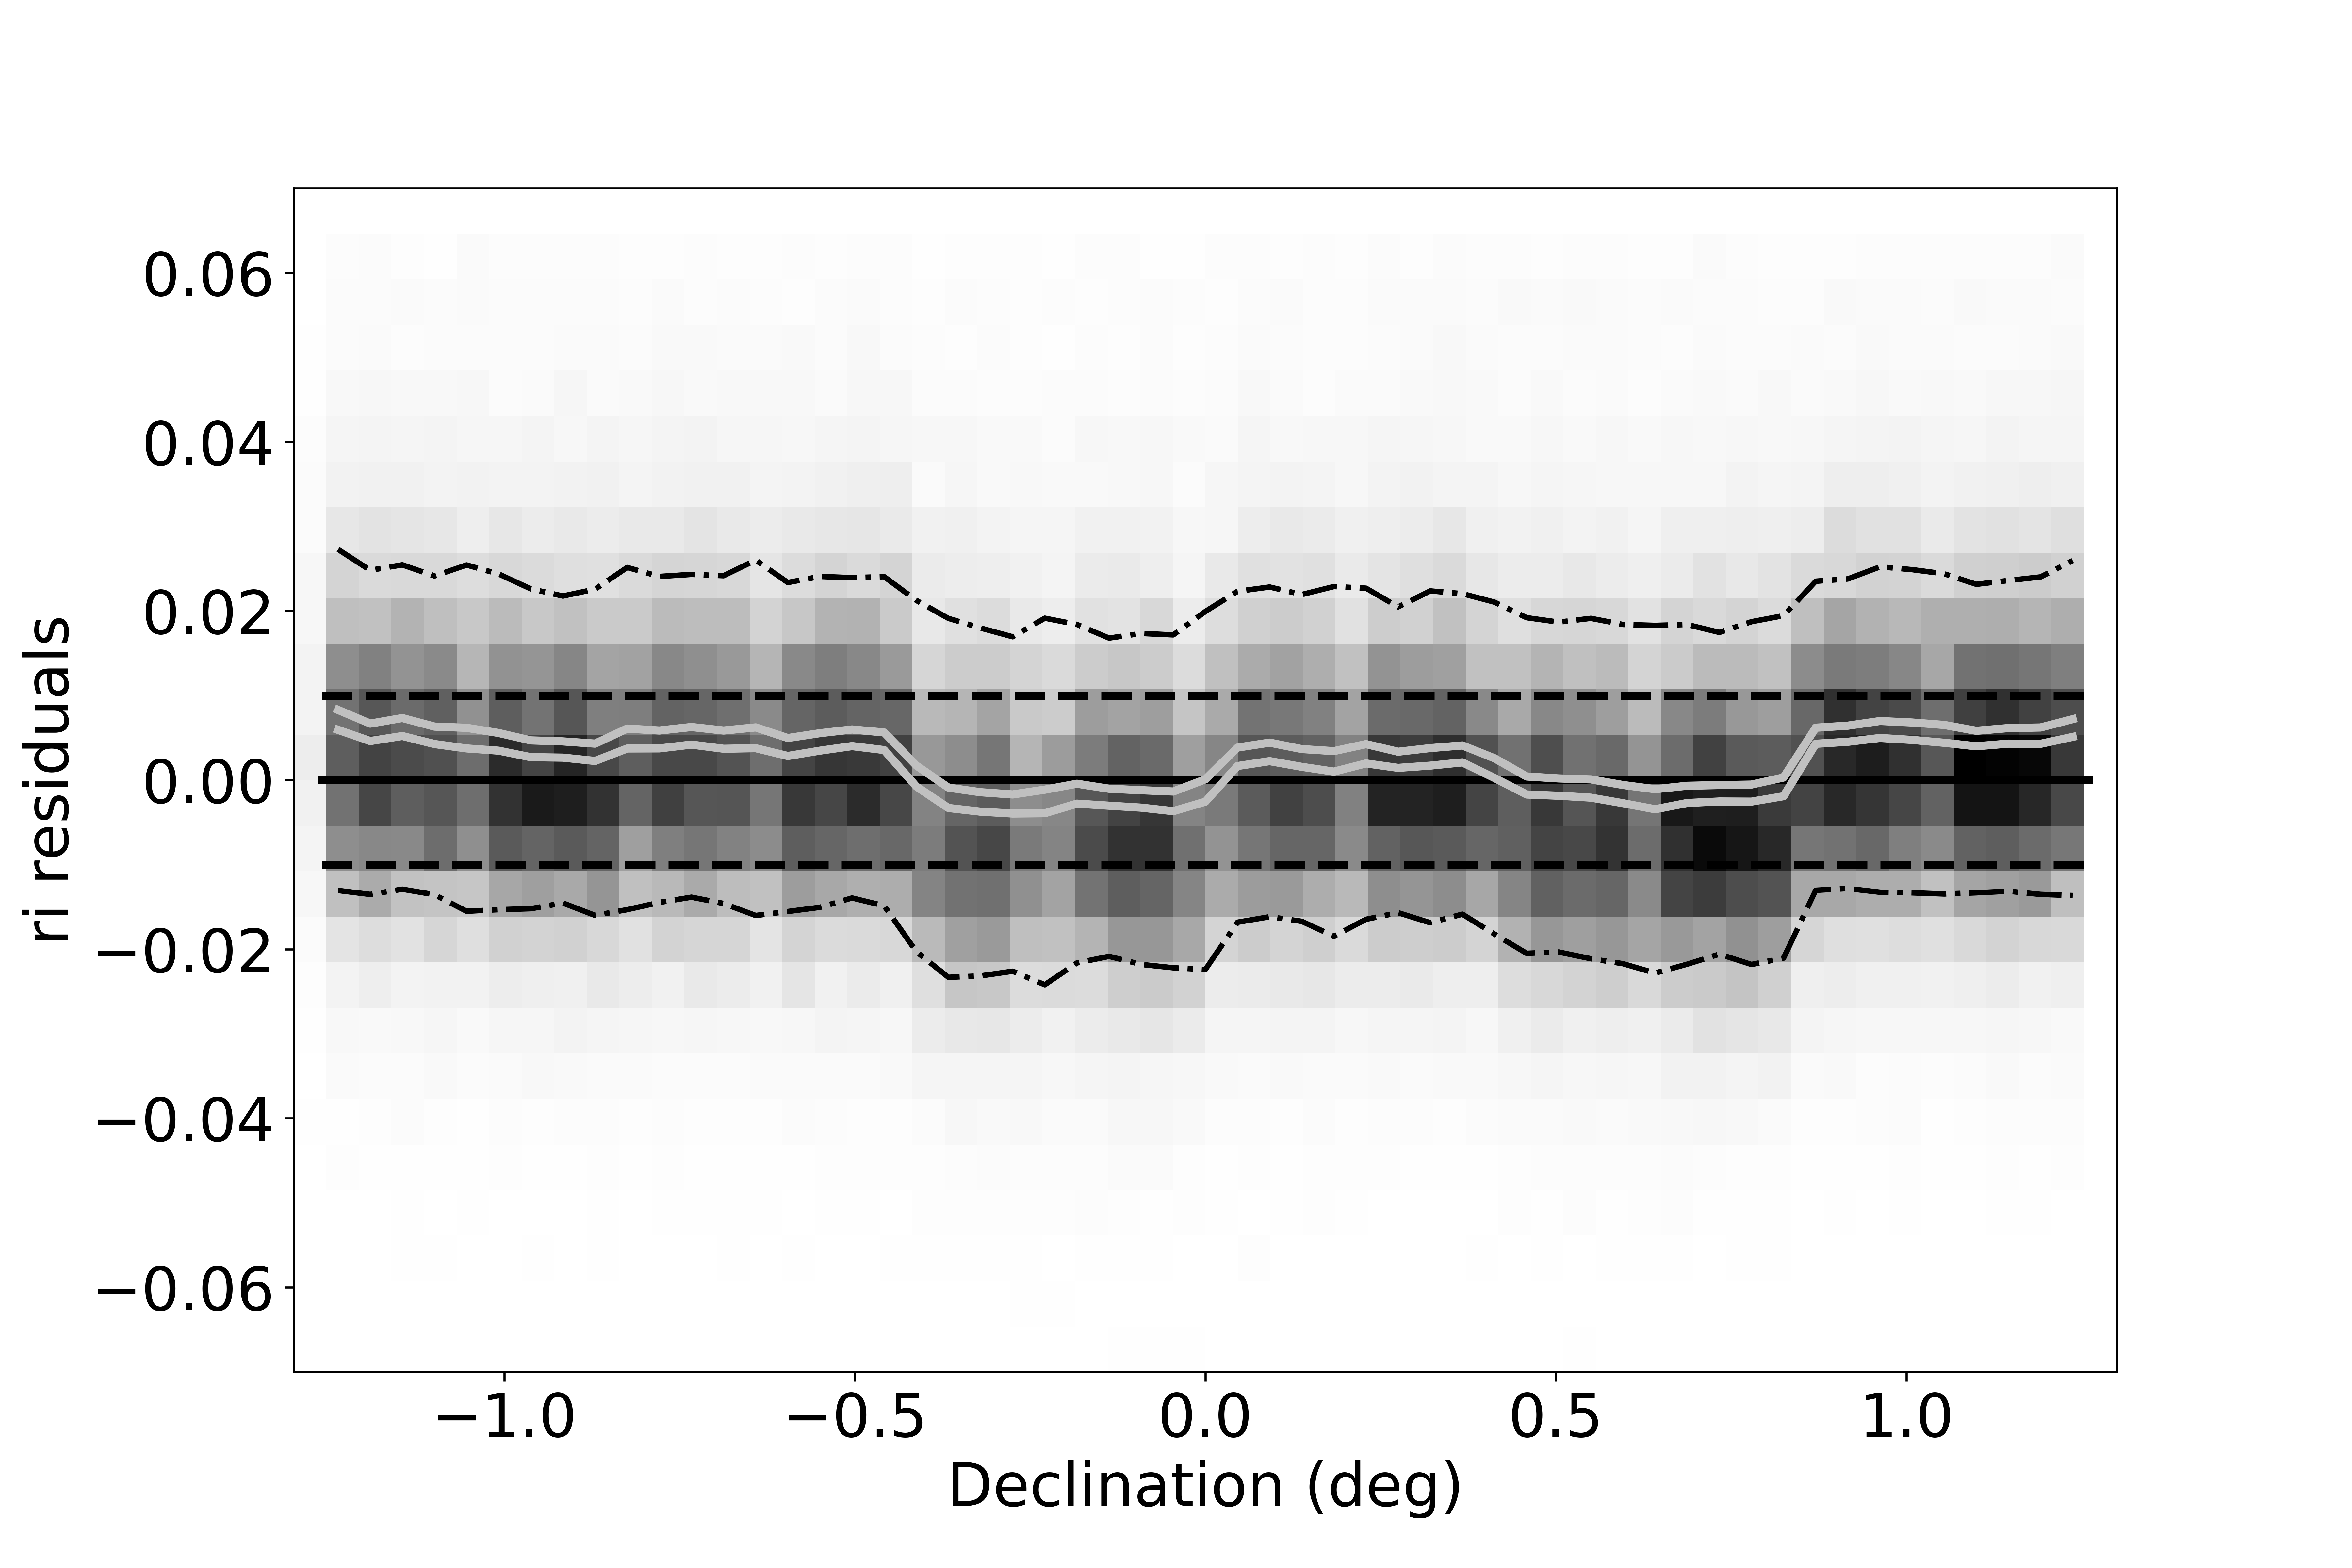
\includegraphics[width=0.9\columnwidth]{figures/colorResidGaiaColorsB_ri_Dec_Hess.png} 
\caption{Analogous to Figure~\ref{fig:graycorrRA} ({\it Right}), except that here residuals 
correspond to differences between the SDSS $r-i$ colour and a synthetic $r-i$ colour
generated using Gaia's $BP-RP$ colour. Note the signature of SDSS camera columns
at the level of a few millimags. The standard deviation for the binned medians is 
3.2 millimag (for other bands, please see Table~\ref{tab:GaiaRMS}.}
\label{fig:riresid}
\end{figure}


The largest corrections were derived for the $u$ band. Given that Gaia's BP-RP
colour does not strongly constrain the $u$ band flux, we used the CFIS catalog 
(see Section~\ref{ssec:cfis}) as an independent verification test. We verified that
zeropoint errors in the SDSS catalog implied by Gaia's and CFIS data agree at the
level a few millimags in Declination direction, but found larger inconsistencies of $\sim$0.01-0.02 mag
 for R.A. bins. For this reason, we only applied the $u$ band 
correction in Declination direction. The plausible $u$ band zeropoint errors in 
the new catalog are further discussed in Section~\ref{sec:CFIStest}. %This final version of the catalog version was labeled v4.2, and it is publicly available\footnote{See \url{http://faculty.washington.edu/ivezic/sdss/catalogs/stripe82.html}}. 

%This final  catalog version was labeled v4.2, and it is also publicly available. 

 %%%%%%%%%%%%%%%%%%%%%%%%%%%%%%%%%%%%%%%%%


\subsubsection{Validation of recalibration  \label{sec:SSCvsGaia}} 
  
By construction, the new v4.2 catalog should not show appreciable zeropoint residuals when 
binned by R.A. and Declination. We have verified this expectation for all colours used in 
recalibration. For illustration, Figure~\ref{fig:grVSgaiaRADec} shows such a test for the $g-r$ 
colour, with binned median scatter of the order 1 millimag. 

\begin{figure*}
    \centering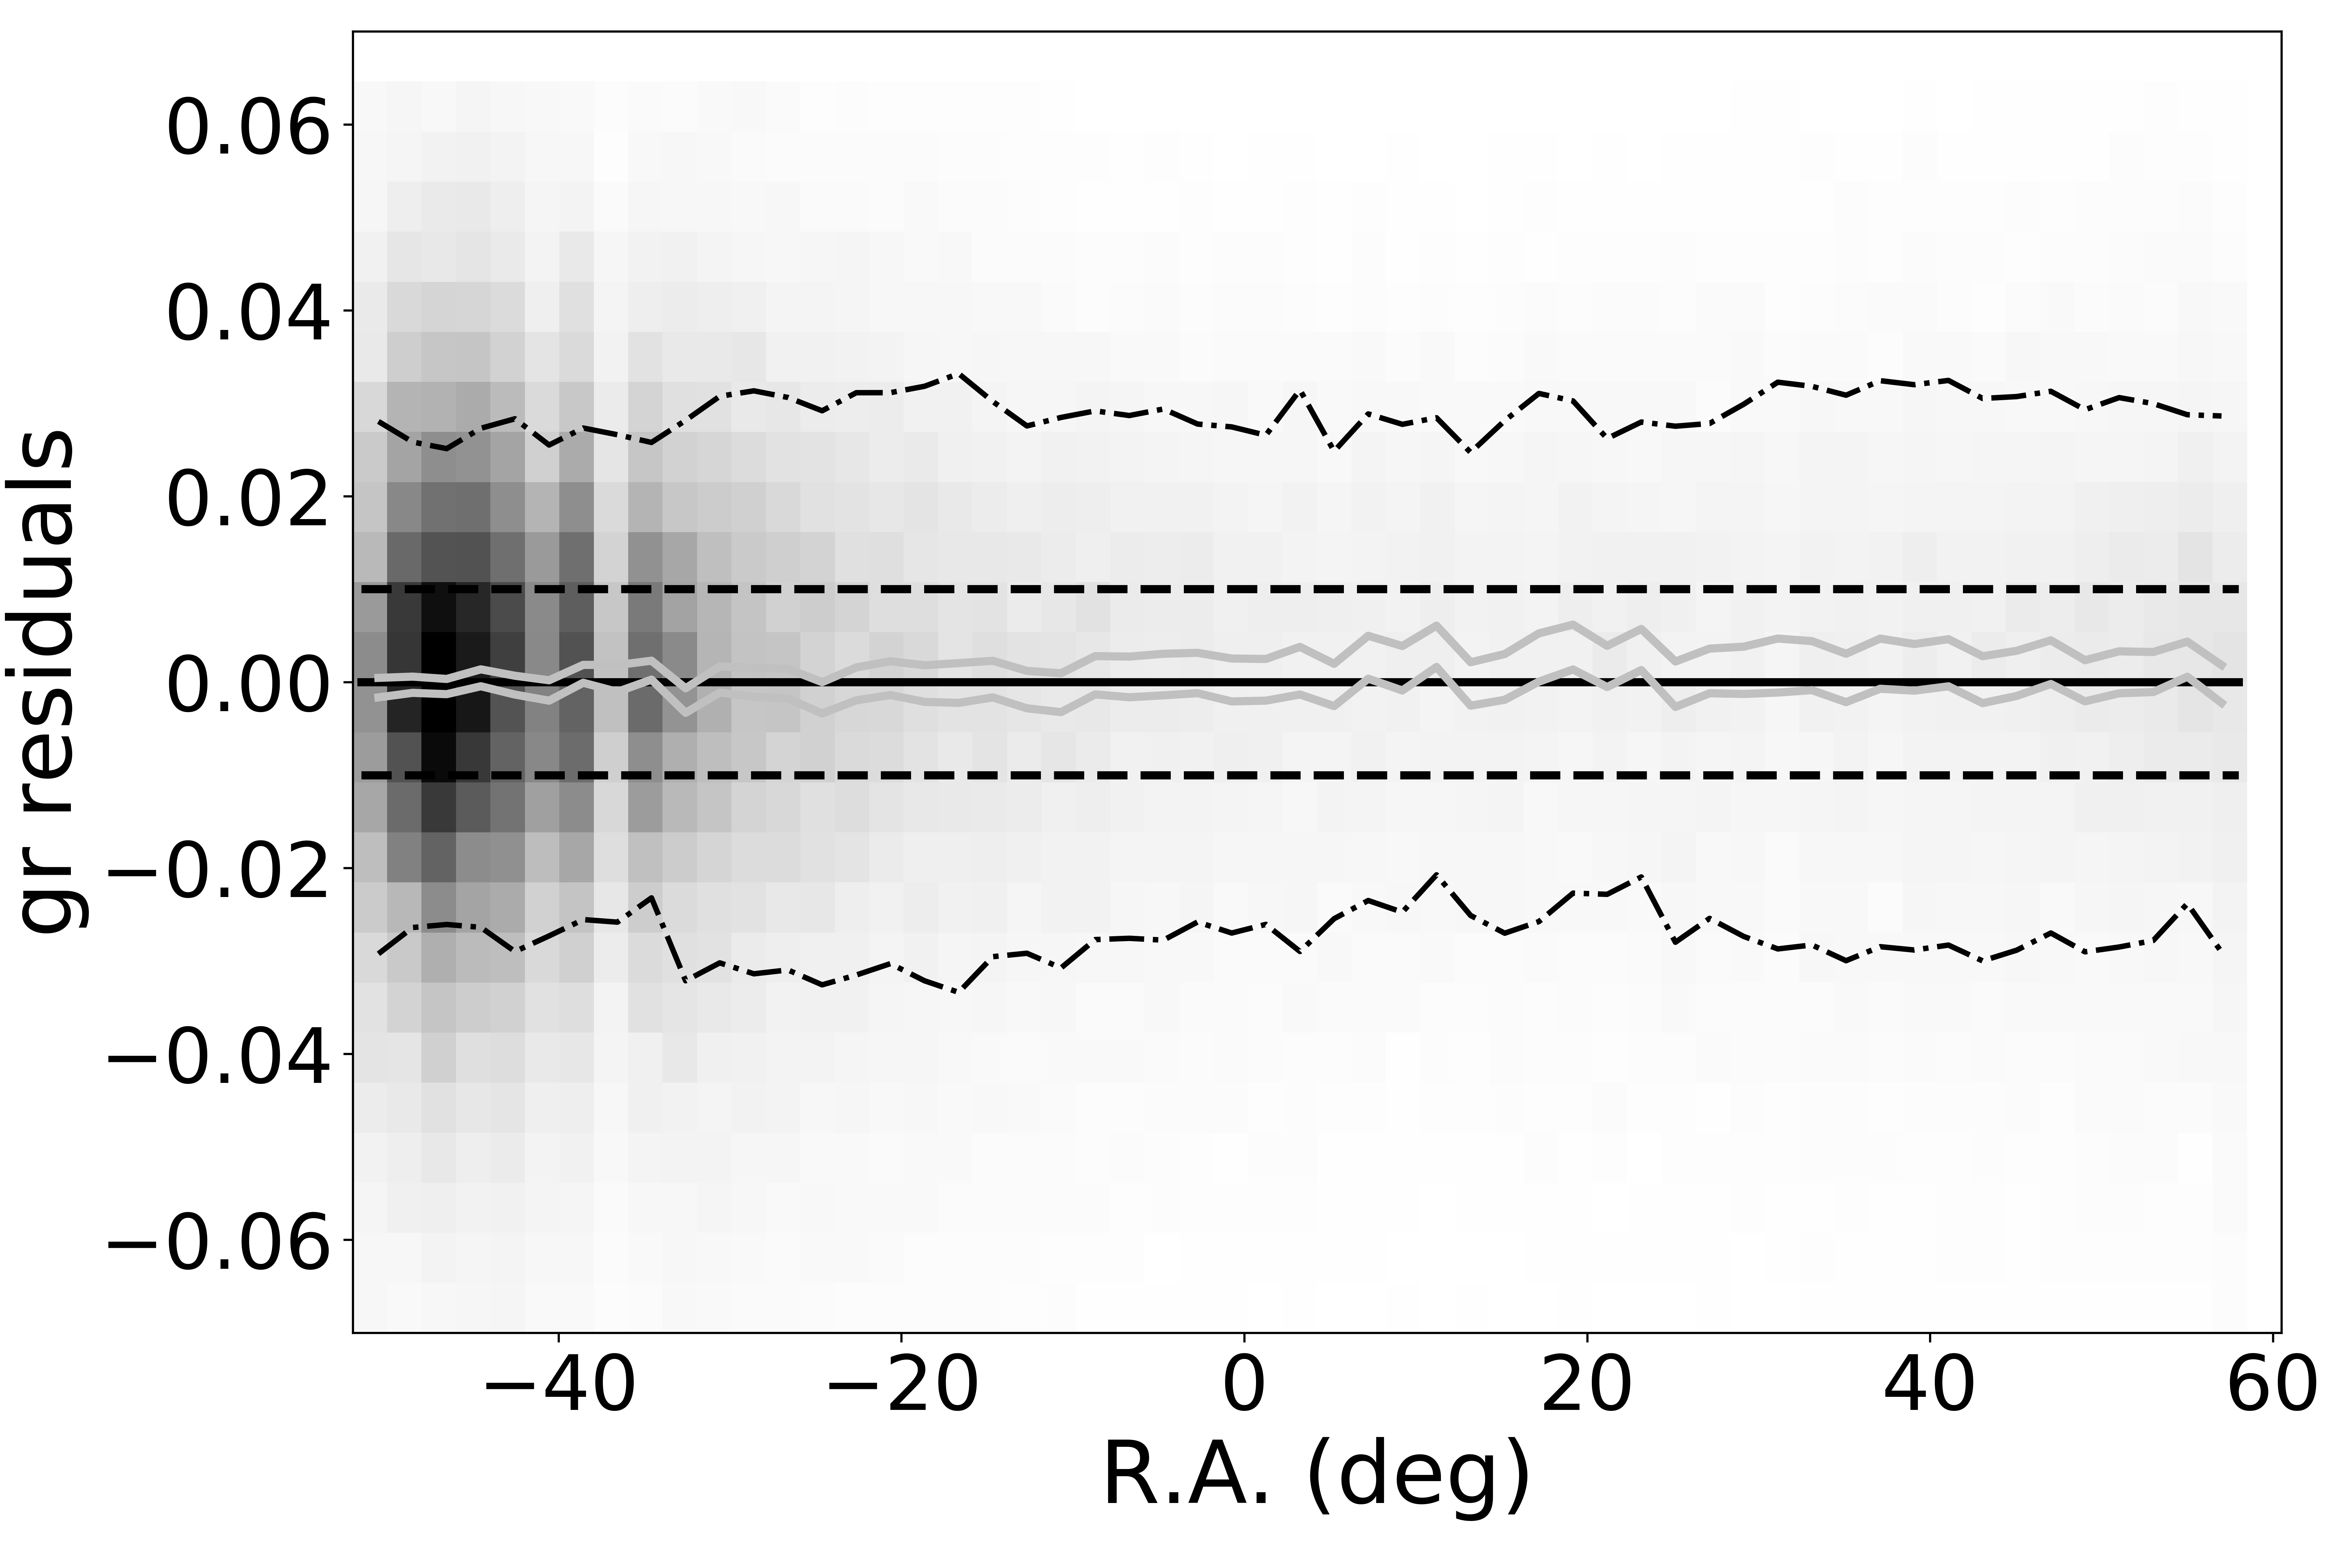
\includegraphics[width=0.45\textwidth]{figures/colorResidGaiaColors_gr_RA_Hess.png} 
    \centering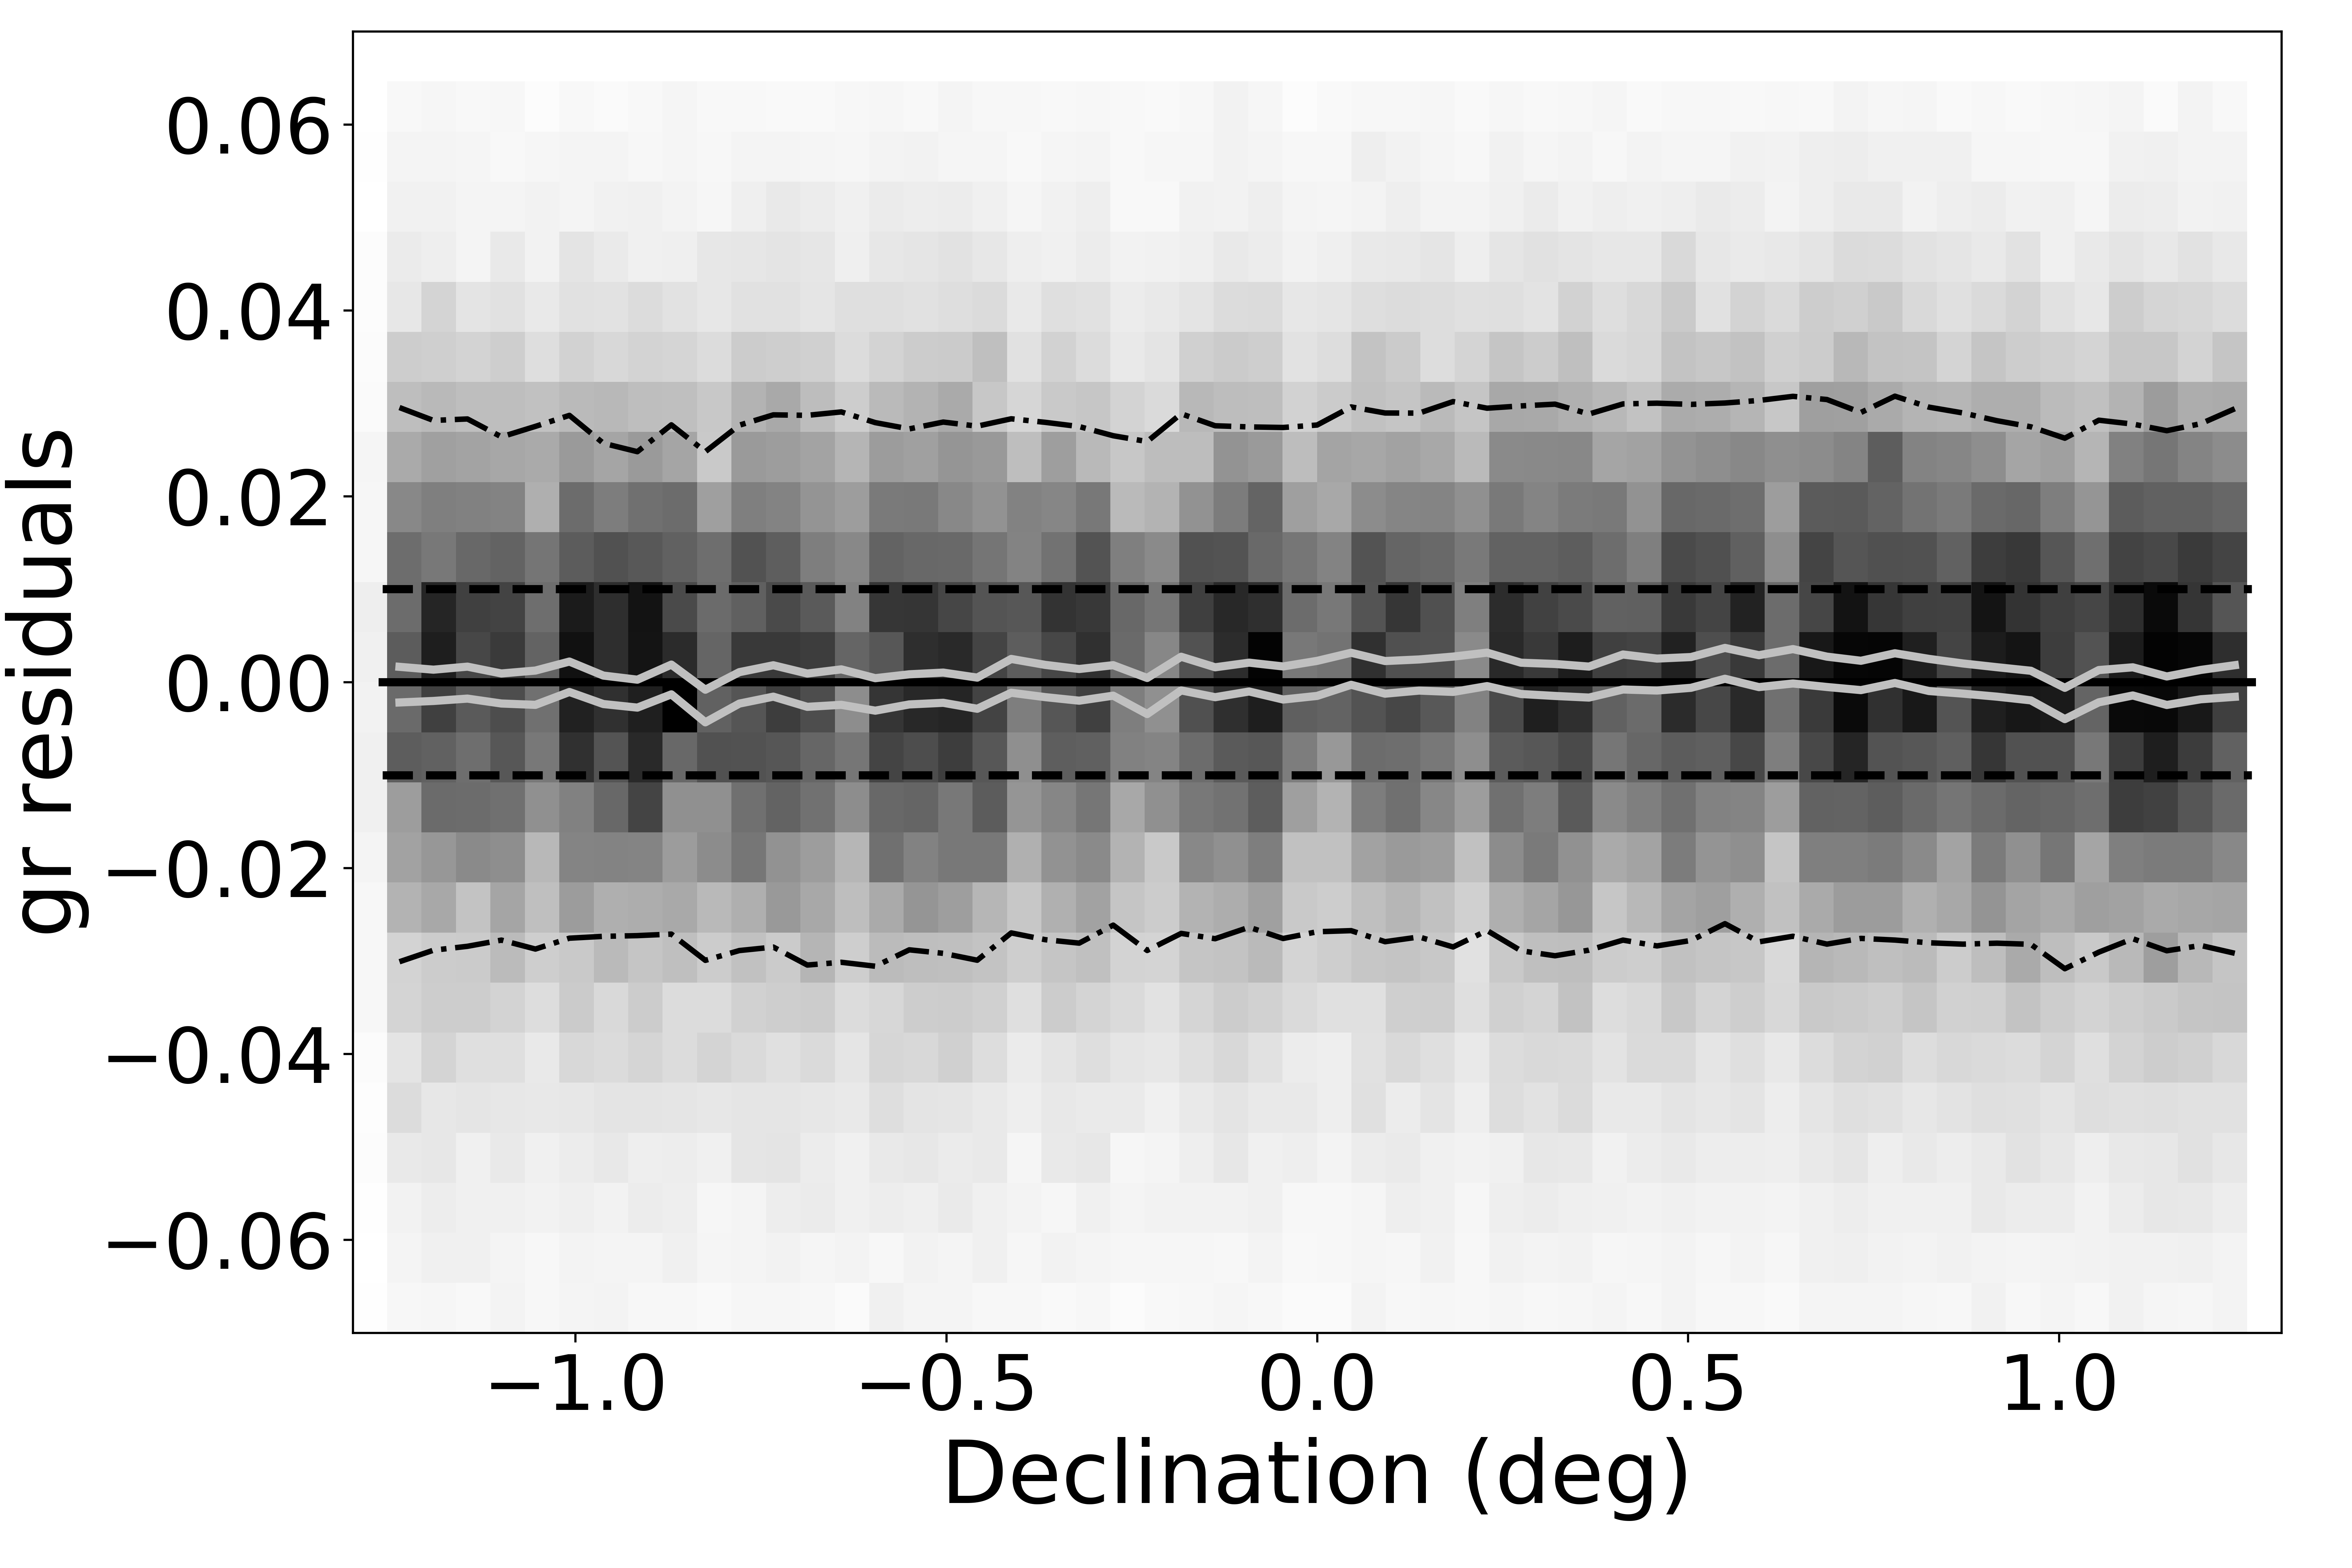
\includegraphics[width=0.45\textwidth]{figures/colorResidGaiaColors_gr_Dec_Hess.png} 
\caption{({\it Left}) Analogous to Figure~\ref{fig:graycorrRA}, except that here residuals between
the SDSS $g-r$ colour from the v4.2 catalog and a synthetic $g-r$ colour generated using 
Gaia's $BP-RP$ colour are shown. The binned median scatter is 1.6 millimag. ({\it Right}) The 
$g-r$ residuals are shown as a function of Declination. The binned median scatter is 
0.8 millimag.}
\label{fig:grVSgaiaRADec}
\end{figure*}
 


%%%%%%%%%%%%%%%%%%%%%%%%%%%%%%%%%%%%%%%%%

\subsection{Comparison of the SDSS v2.6 and v4.2 catalogs \label{sec:v26v42}} 

The v2.6 (``old'') SDSS Standard Star \pOc has been extensively used 
\citep[e.g.,][]{2008AJ....135..338F},
and here we briefly analyze differences between the v4.2 (``new'') and v2.6 magnitudes
to inform the future users about catalog consistency. 
In our analysis, we first compare v2.6 and v4.2 magnitudes of individual stars and 
bin the differences by R.A., Declination and magnitude. 

On average, both catalog versions are on the same magnitude scale (the median $ugriz$ 
magnitude differences for all stars are zero by construction). There are no systematic offsets 
when binned by magnitude, as illustrated in Figure~\ref{fig:v26v34drr}. The most obvious 
differences appear when magnitude differences are binned by Declination. An example is 
shown in Figure~\ref{fig:v26v34drDec}, where the periodicity of residuals corresponds to the 
field-of-view size for the SDSS Photometric Telescope \citep{2006AN....327..821T}. 
The standard deviation for median values per bin is 6.8 millimag, with extreme values about 
0.01 mag. It is likely that systematic errors in the calibration star network photometry 
were propagated through ``flat-field corrections'' discussed by \pO\ to the v2.6 catalog.
We note that these errors, now found thanks to Gaia catalogs, are well within the claimed
photemetric accuracy by both \pO\ and \cite{2002AJ....123.2121S}. The standard deviation 
for median values per bin for all bands and both coordinates is listed in Table~\ref{tab:oldnewRMS}. 


% \begin{deluxetable}{l|c|c}[ht!]
% \tablecaption{The robust standard deviation for magnitude differences between the v2.6 (old)
% and v4.2 (new) catalogs. \label{tab:oldnewRMS}}
% \tablehead{
% \colhead{Band} & \colhead{RMS for R.A.} & \colhead{RMS for Dec}
% }
% \startdata
%    NOTE NOTE NOTE: these values are for v4.2 catalog 
%        $u$        &        2.3$^a$    &    25.5      \\
%        $g$        &        4.5    &      9.4      \\  
%        $r$         &        2.0    &      7.0      \\  
%        $i$         &        5.3    &      6.5      \\ 
%        $z$        &        8.9    &      8.4      \\ 
% \enddata
% \tablenotetext{a}{For the $u$ band, the scatter in R.A. direction is due to more observations
% in v4.2 than in v2.6, rather than zeropoint correction.} 
% \end{deluxetable}
   
\begin{table}
	\centering
	\caption{The robust standard deviation for magnitude differences between the v2.6 (old) and v4.2 (new) catalogs.}
	\label{tab:oldnewRMS}
	\begin{tabular}{l|c|c} % 
		\hline
		Band & RMS for R.A. & RMS for Dec \\
		\hline
       % ZI updated to v4.2 catalog 
       $u$        &        2.0$^a$    &    25.5      \\
       $g$        &        4.0    &      9.7      \\  
       $r$         &        1.7    &      7.1      \\  
       $i$         &        4.1    &      6.5      \\ 
       $z$        &        7.5    &      8.4      \\ 
		\hline
	\end{tabular}
     \vspace{1ex}

     {\raggedright {\bf Notes}: (a) For the $u$ band, the scatter in R.A. direction is due to more observations in v4.2 than in v2.6, rather than zeropoint correction.. \par}
\end{table}


\begin{figure}
    \centering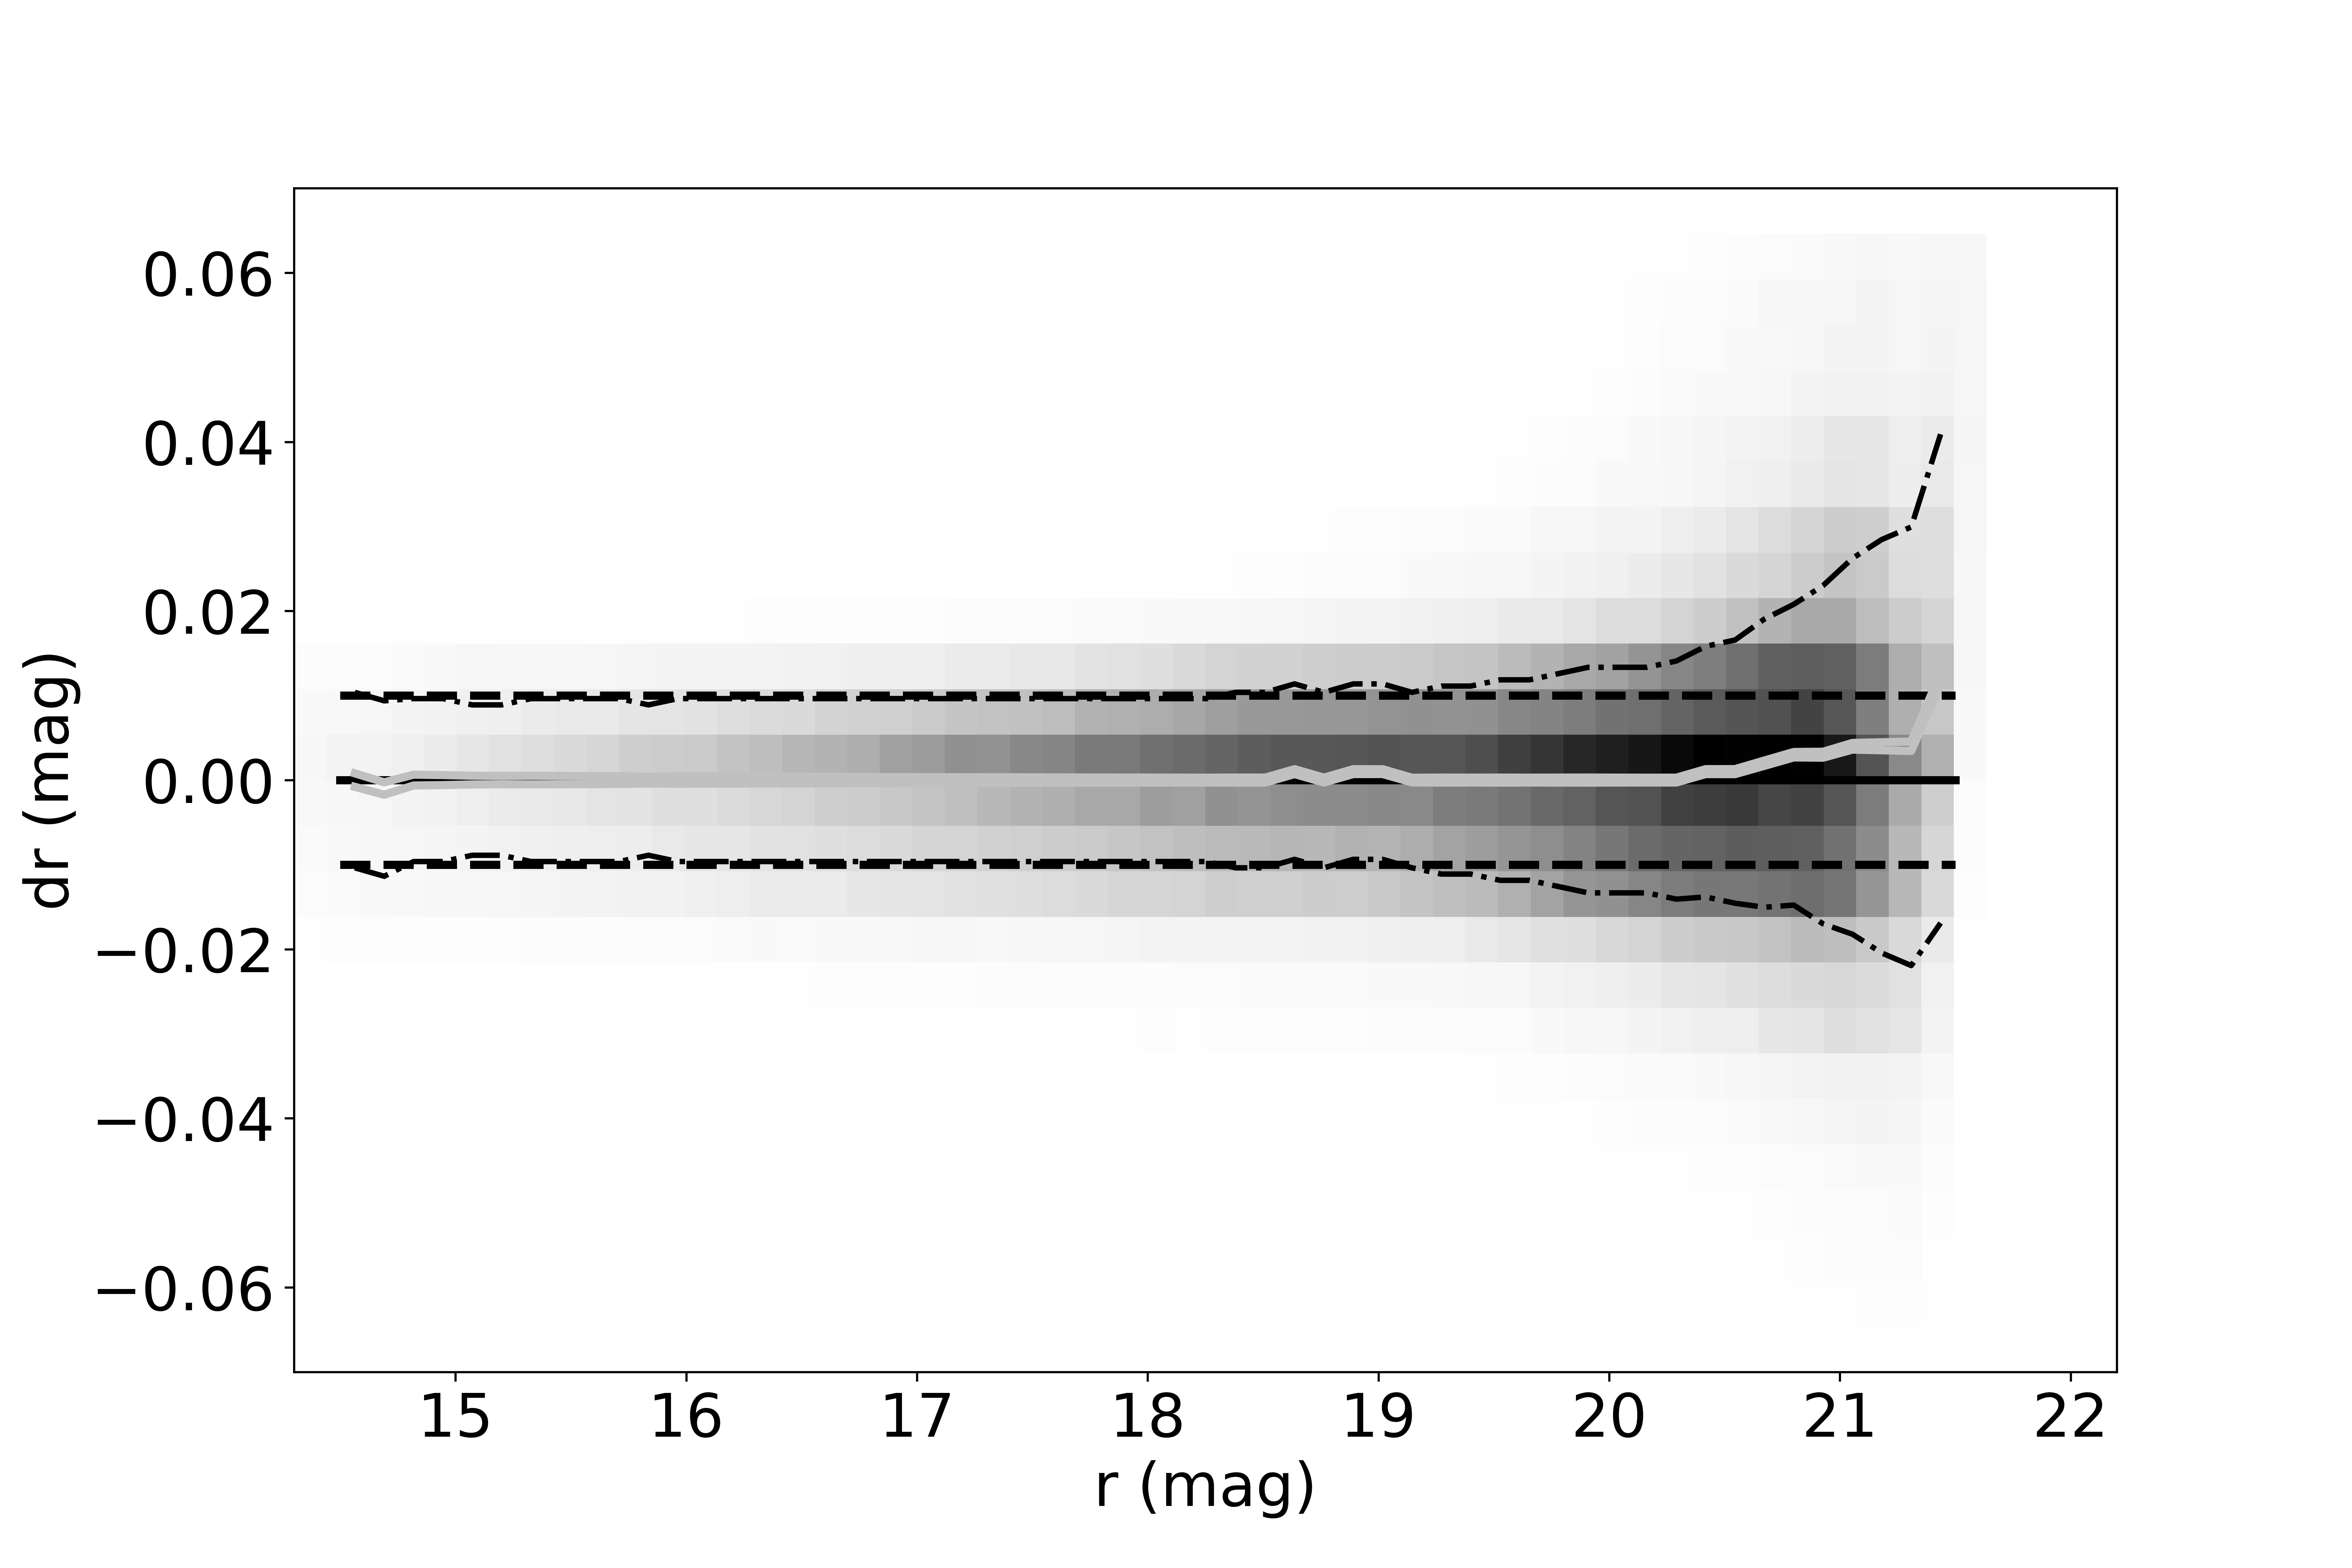
\includegraphics[width=0.95\columnwidth]{figures/testV26vsV42_r_dr_r_mag_Hess.png} 
\caption{The differences between $r$ band magnitudes listed in the v2.6 and v4.2 
SDSS Standard Star catalogs,  shown as a function of the $r$ band magnitude. The 
scatter of median values per bin is 1.7 millimag. The scatter of individual values is 
$\sim0.01$ mag for $r<20$, and it is due to more data in the new catalog.} 
\label{fig:v26v34drr}
\end{figure}


\begin{figure}
    \centering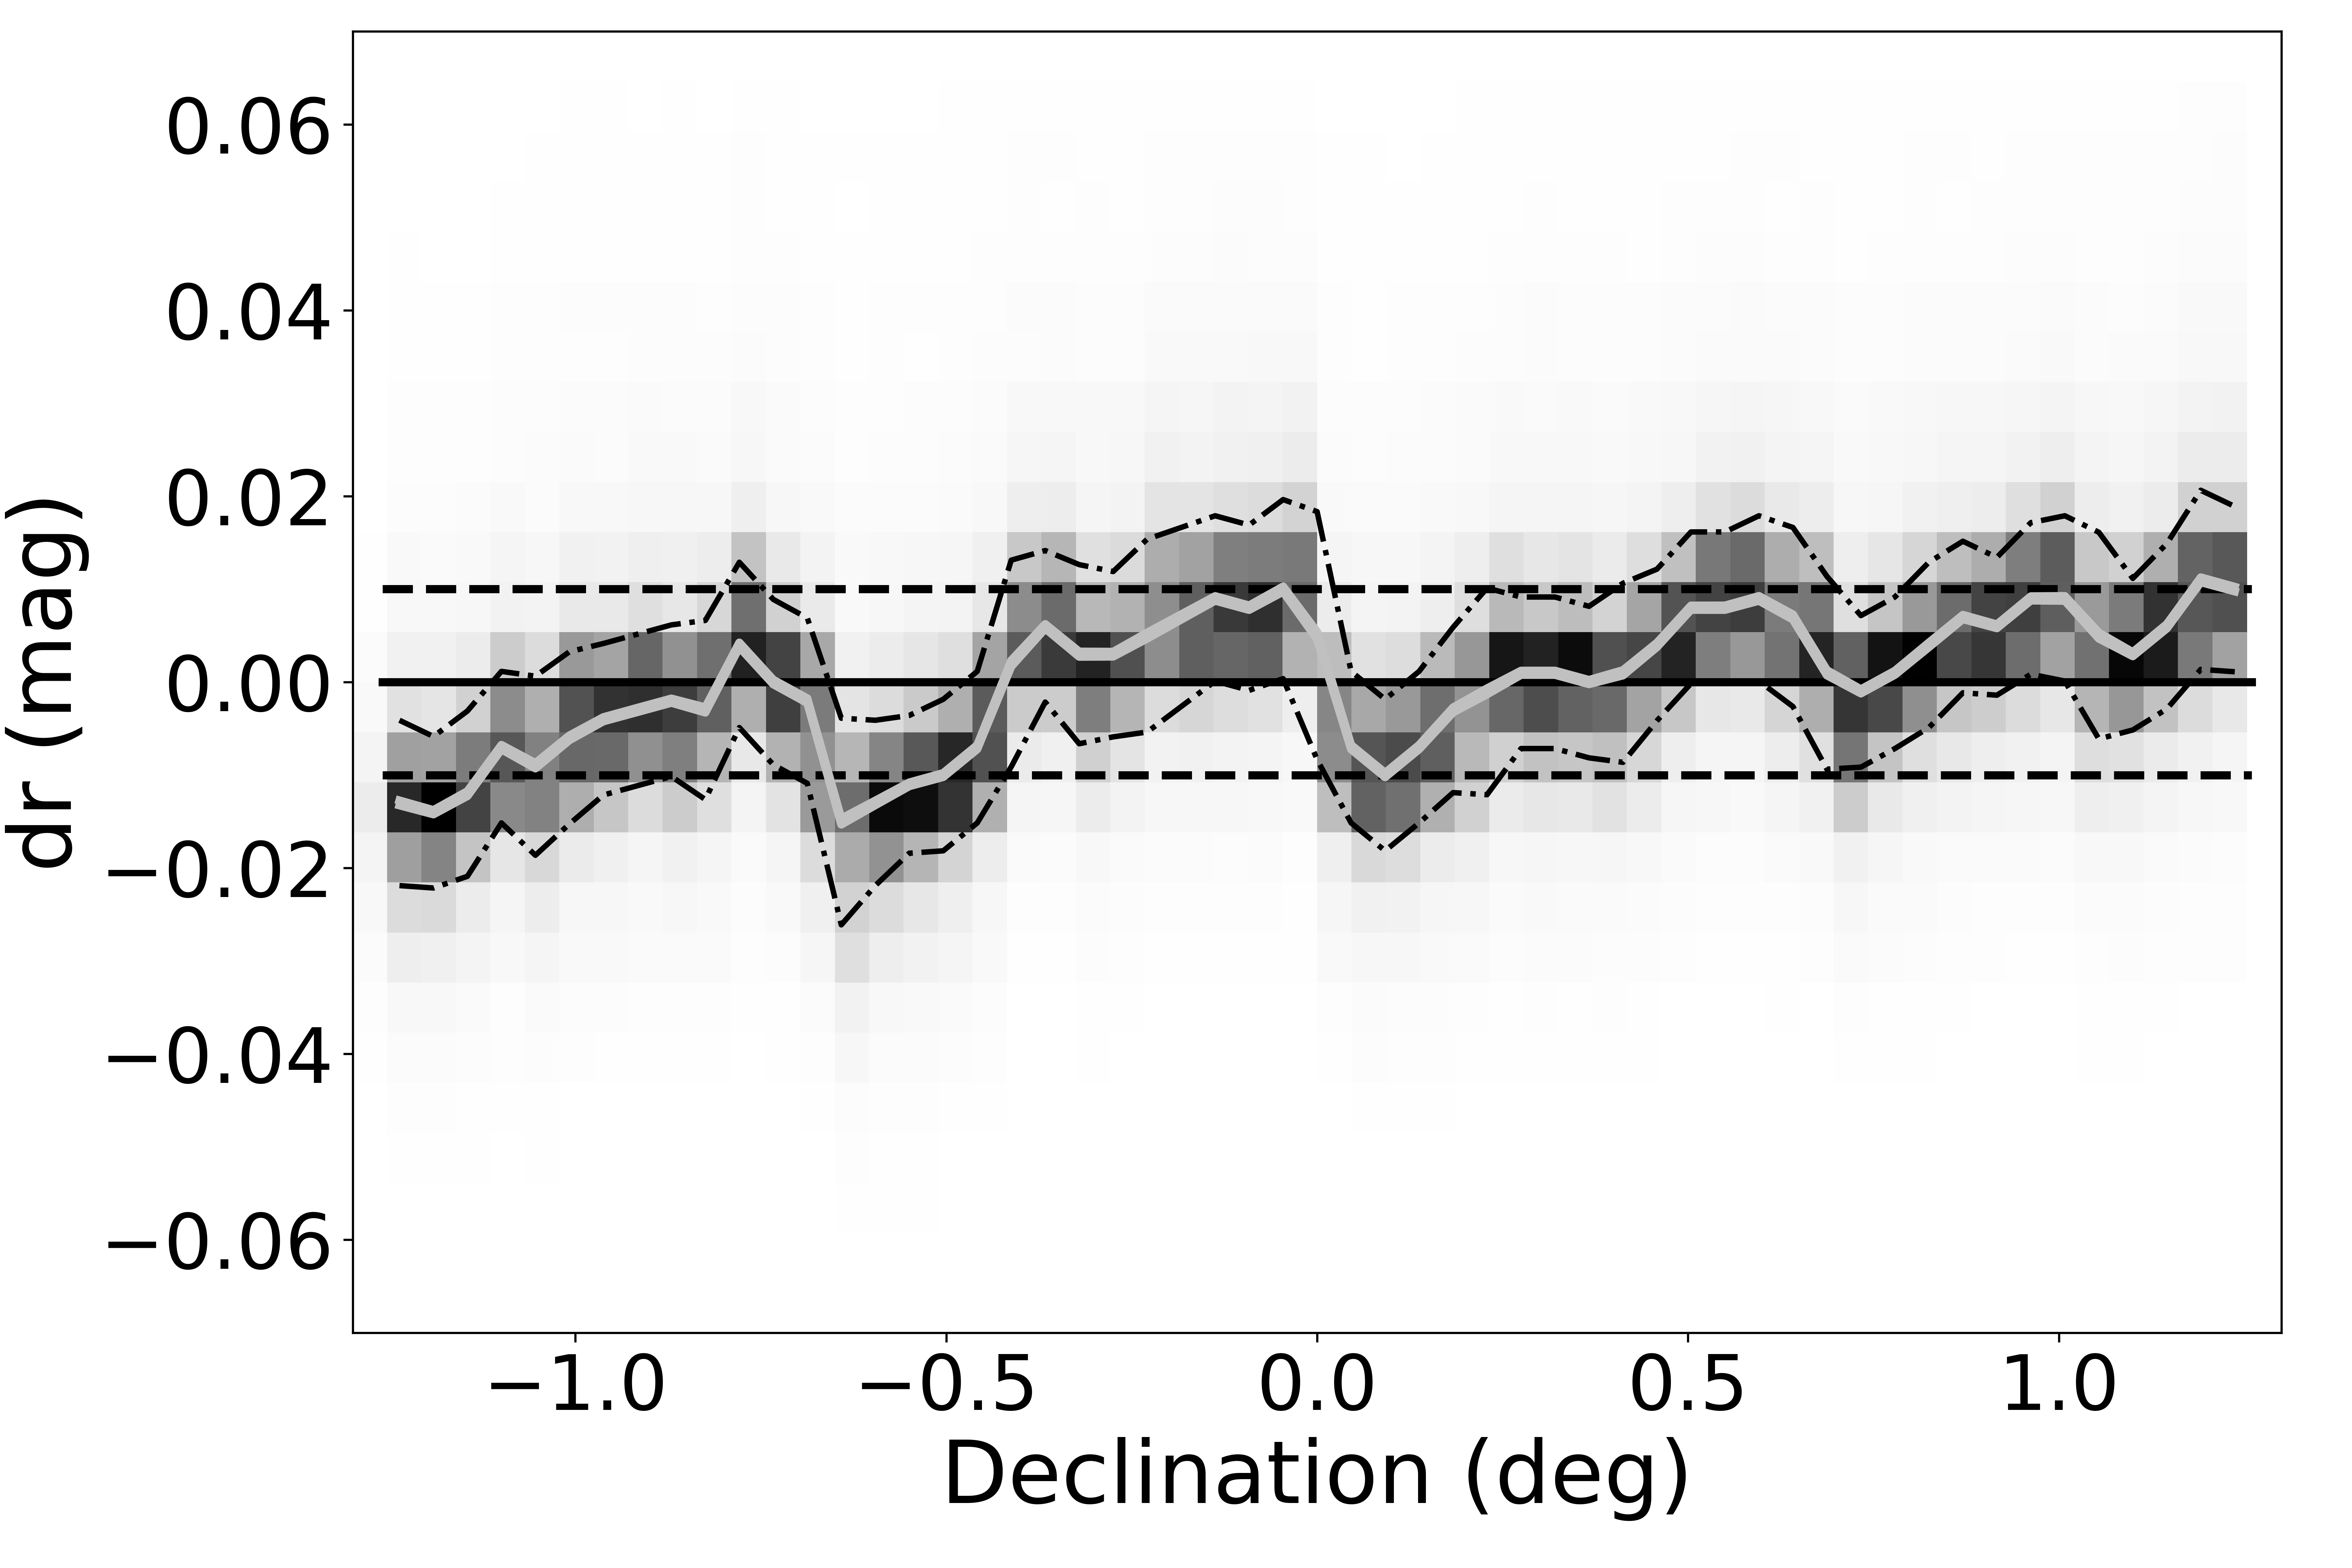
\includegraphics[width=0.95\columnwidth]{figures/testV26vsV42_r_dr_Dec_Hess.png} 
\caption{Analogous to Figure~\ref{fig:v26v34drr}, except that here the $r$ band
differences are shown as a function of Declination (cross-scan direction). The size 
of the four regions corresponds to the field-of-view size of the SDSS Photometric Telescope \citep{2006AN....327..821T}. 
The standard deviation for median values per bin is 7.1 millimag, with extreme values about 
0.01 mag. The scatter of binned medians in R.A. direction is much smaller -- 1.7 millimag. 
For statistics in other bands, please see Table~\ref{tab:oldnewRMS}.}
\label{fig:v26v34drDec}
\end{figure}
 

Given the quality of Gaia photometry, there should be no doubt that SDSS $ugriz$ photometry
reported in the new v4.2 catalog is superior to the old v2.6 catalog. Nevertheless, we perform
additional tests, based on the position of the stellar locus in the $g-r$ vs. $u-g$, $r-i$ vs. $g-r$ 
and $i-z$ vs. $r-i$ colour-colour diagrams  \citep{2004AN....325..583I}. The tests are based
on the second principal colour for the blue part of the stellar locus, whose median should 
not deviate from zero by construction. Figure~\ref{fig:comparew} compares the behavior
of the $w$ colour for the old v2.6 and new v4.2 catalog and demonstrates that the $gri$
photometry is better calibrated in the latter. The behavior of the $s$ and $y$ colours for the 
new catalog is shown in Figure~\ref{fig:comparesy}. {\it Based on these tests, we find that 
the contribution of the zeropoint errors is $<5$ millimag to $gri$ photometry, and 
$<10$ millimag for the $u$ and $z$ bands.} 



\begin{figure*}
    \centering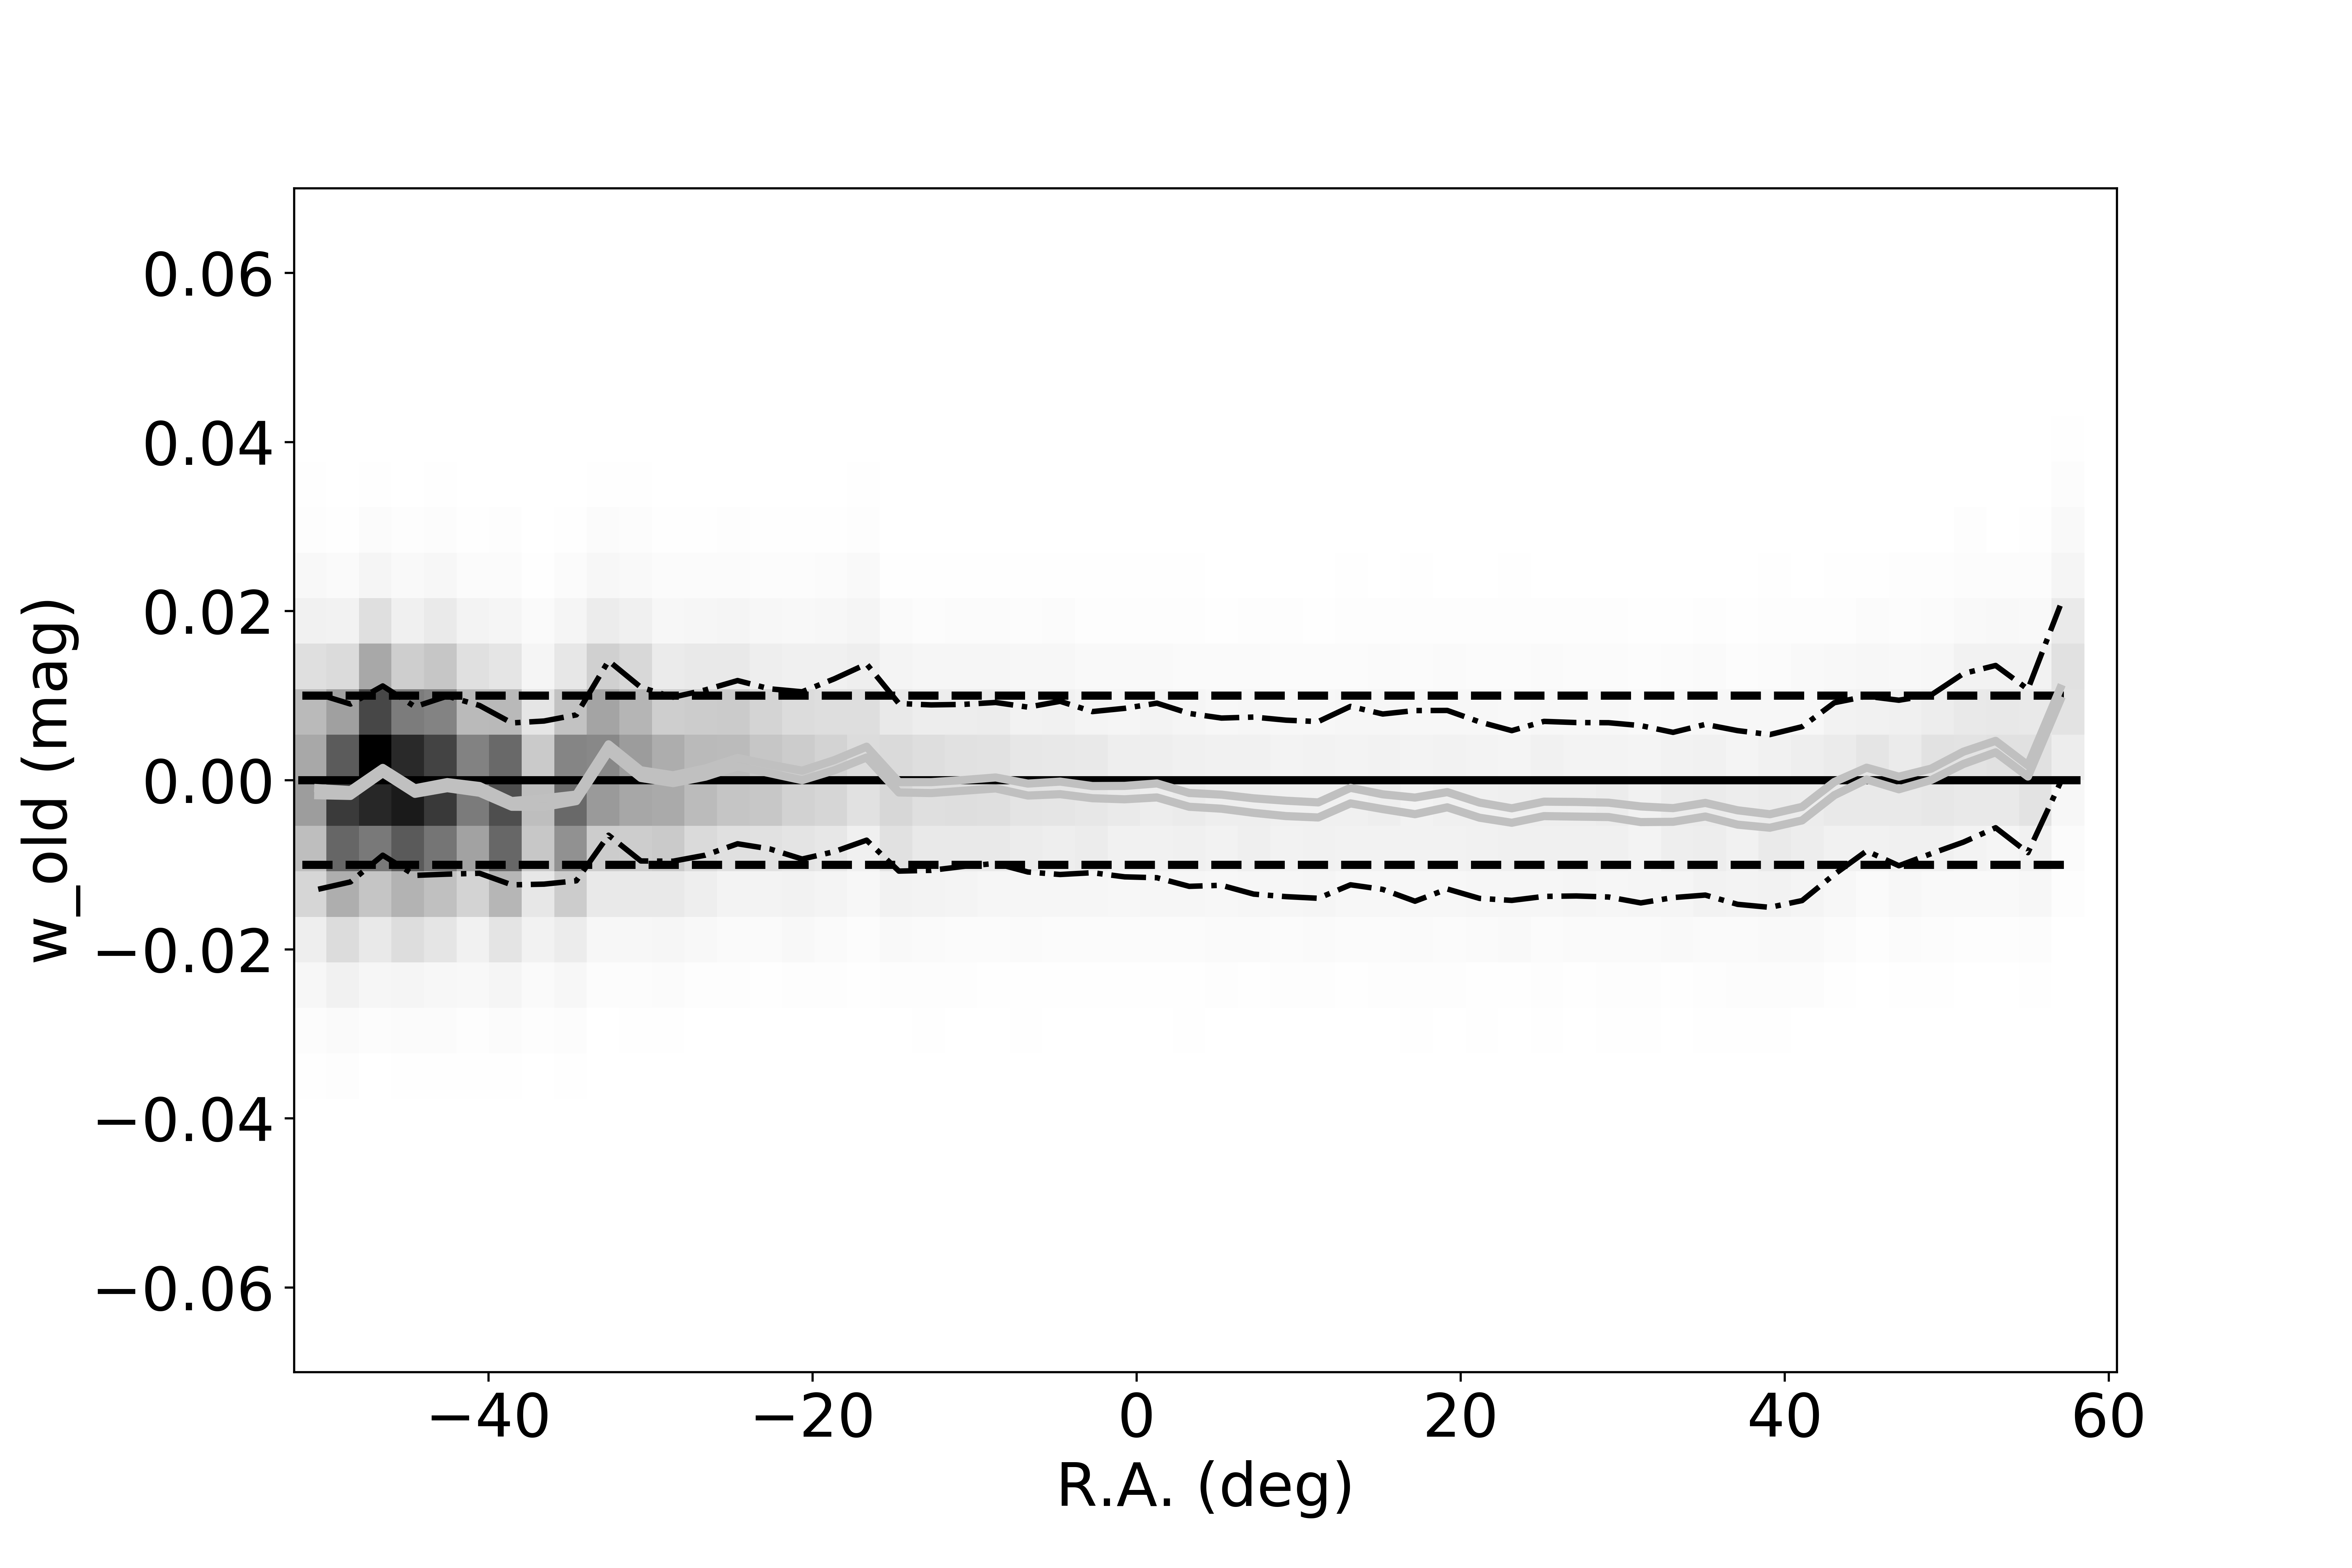
\includegraphics[width=0.45\textwidth]{figures/testV26vsV42_r_w_old_RA_Hess.png}
    \centering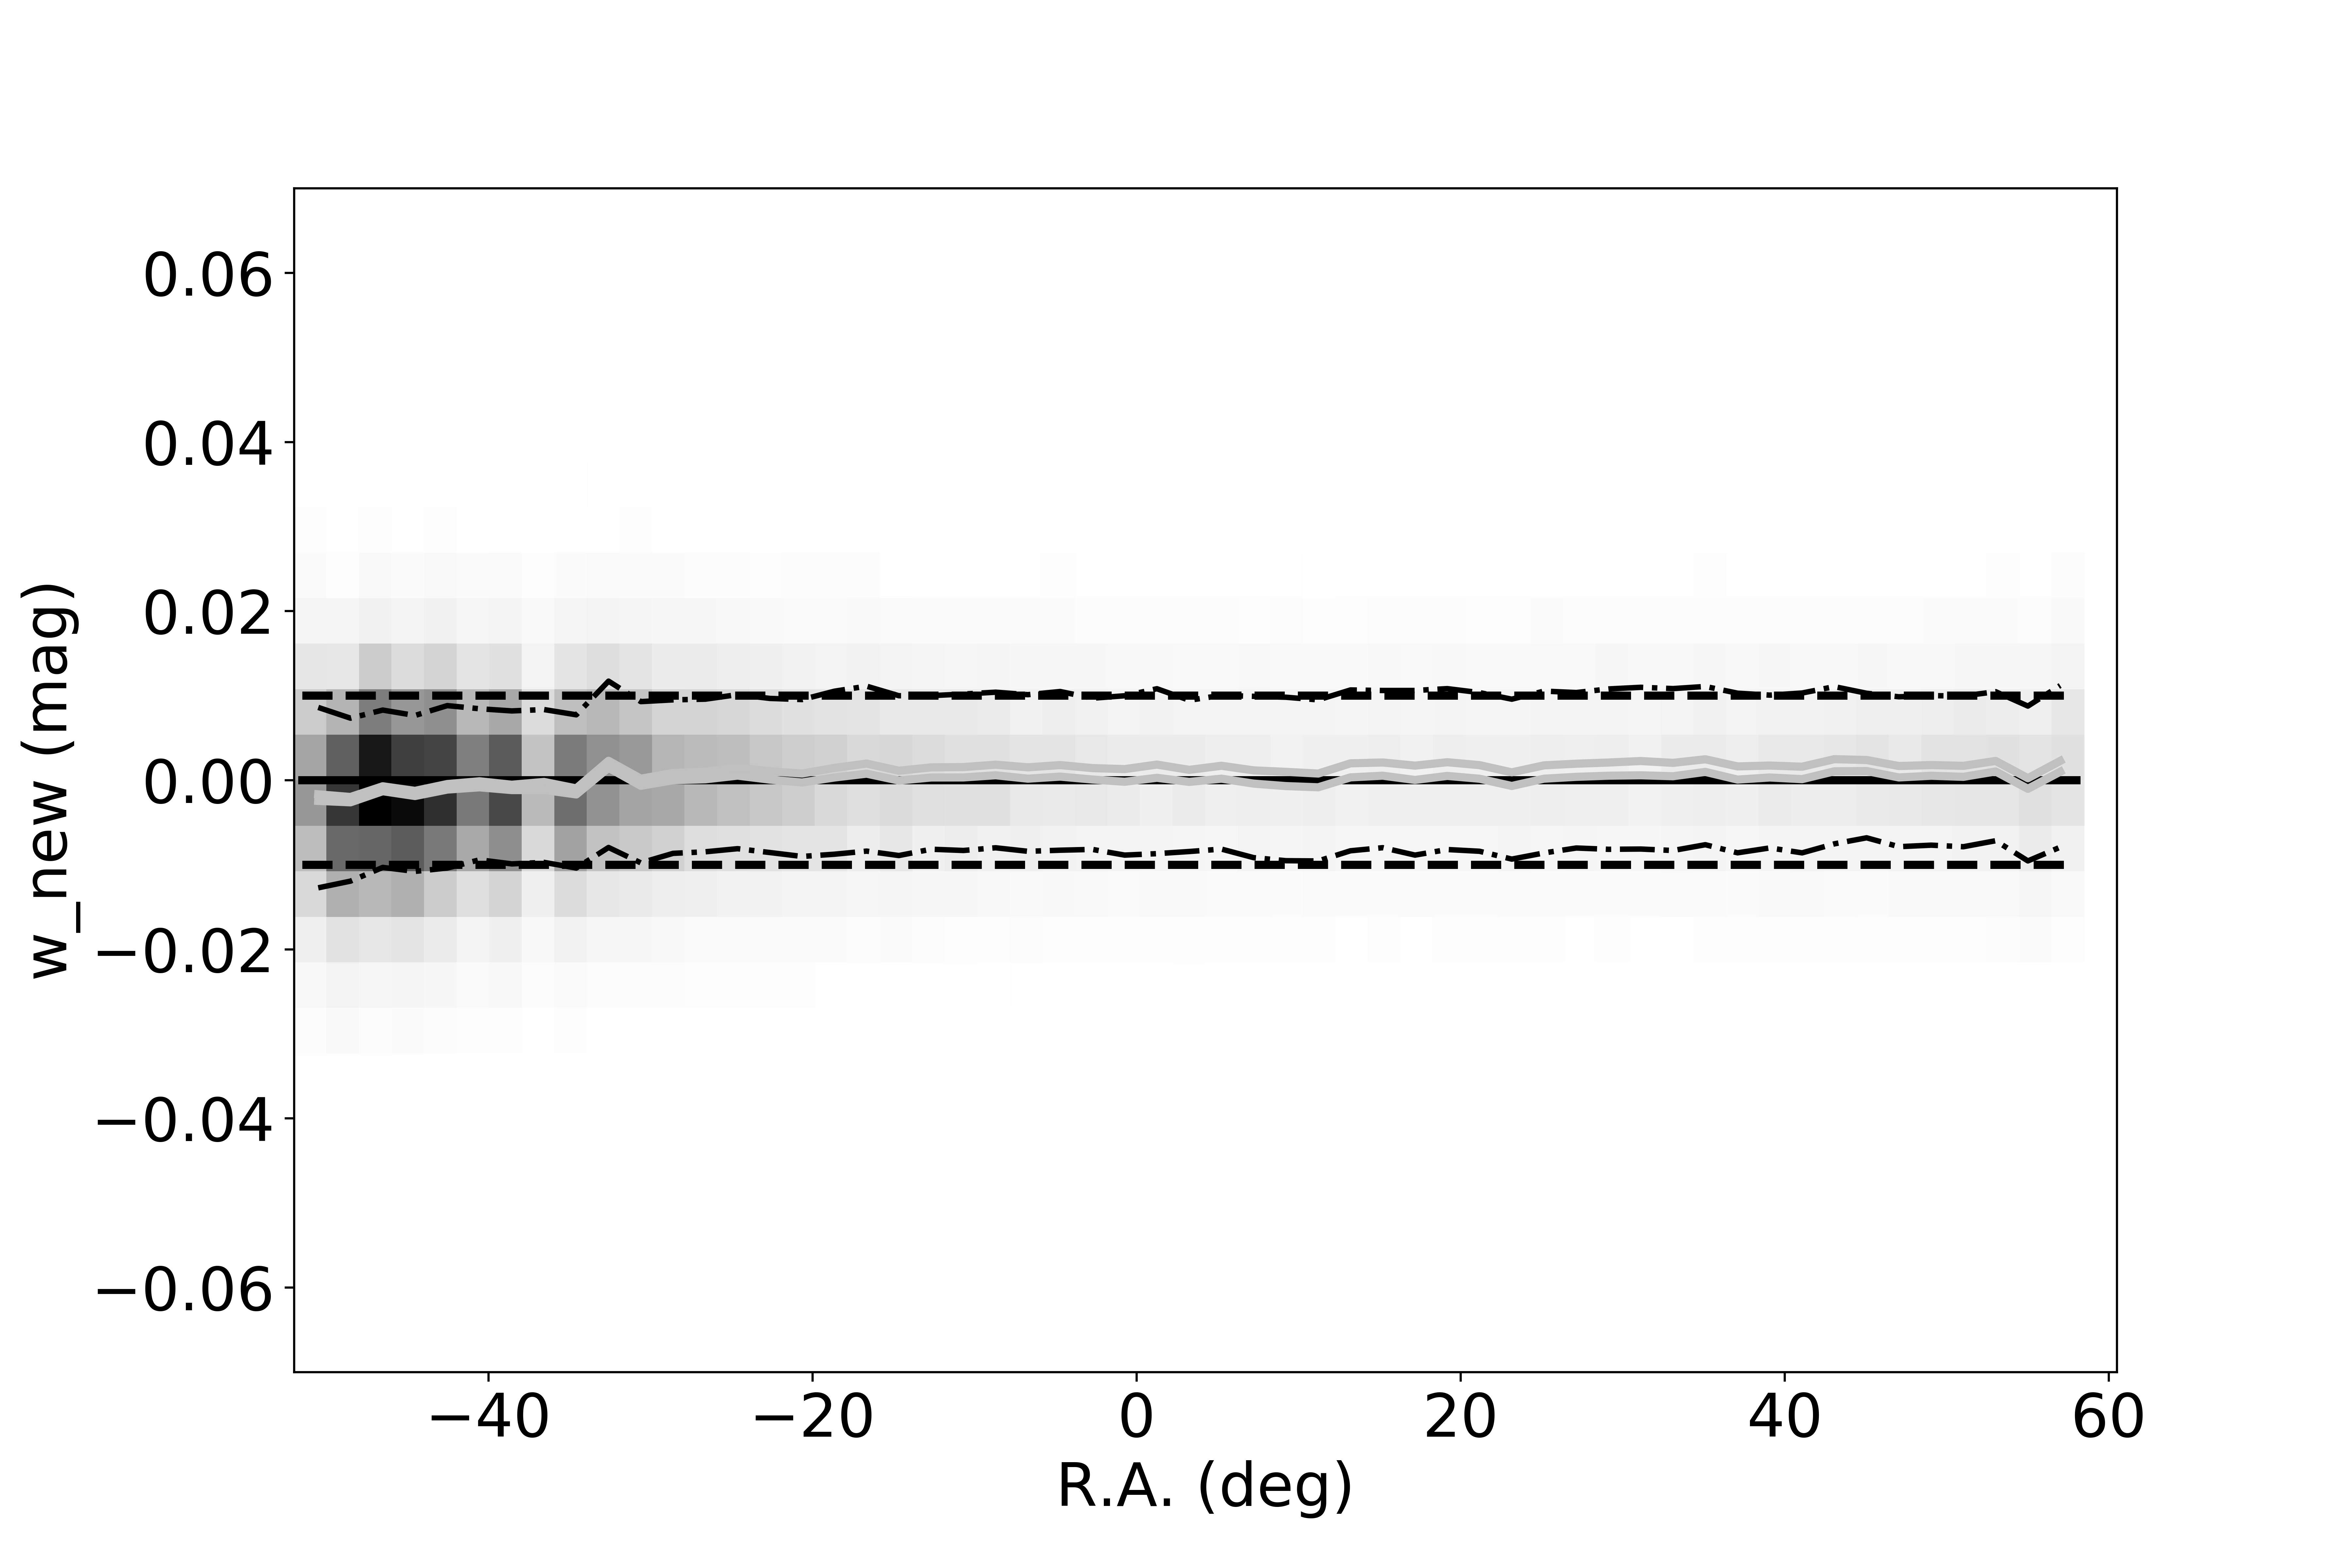
\includegraphics[width=0.45\textwidth]{figures/testV26vsV42_r_w_new_RA_Hess.png}
    \centering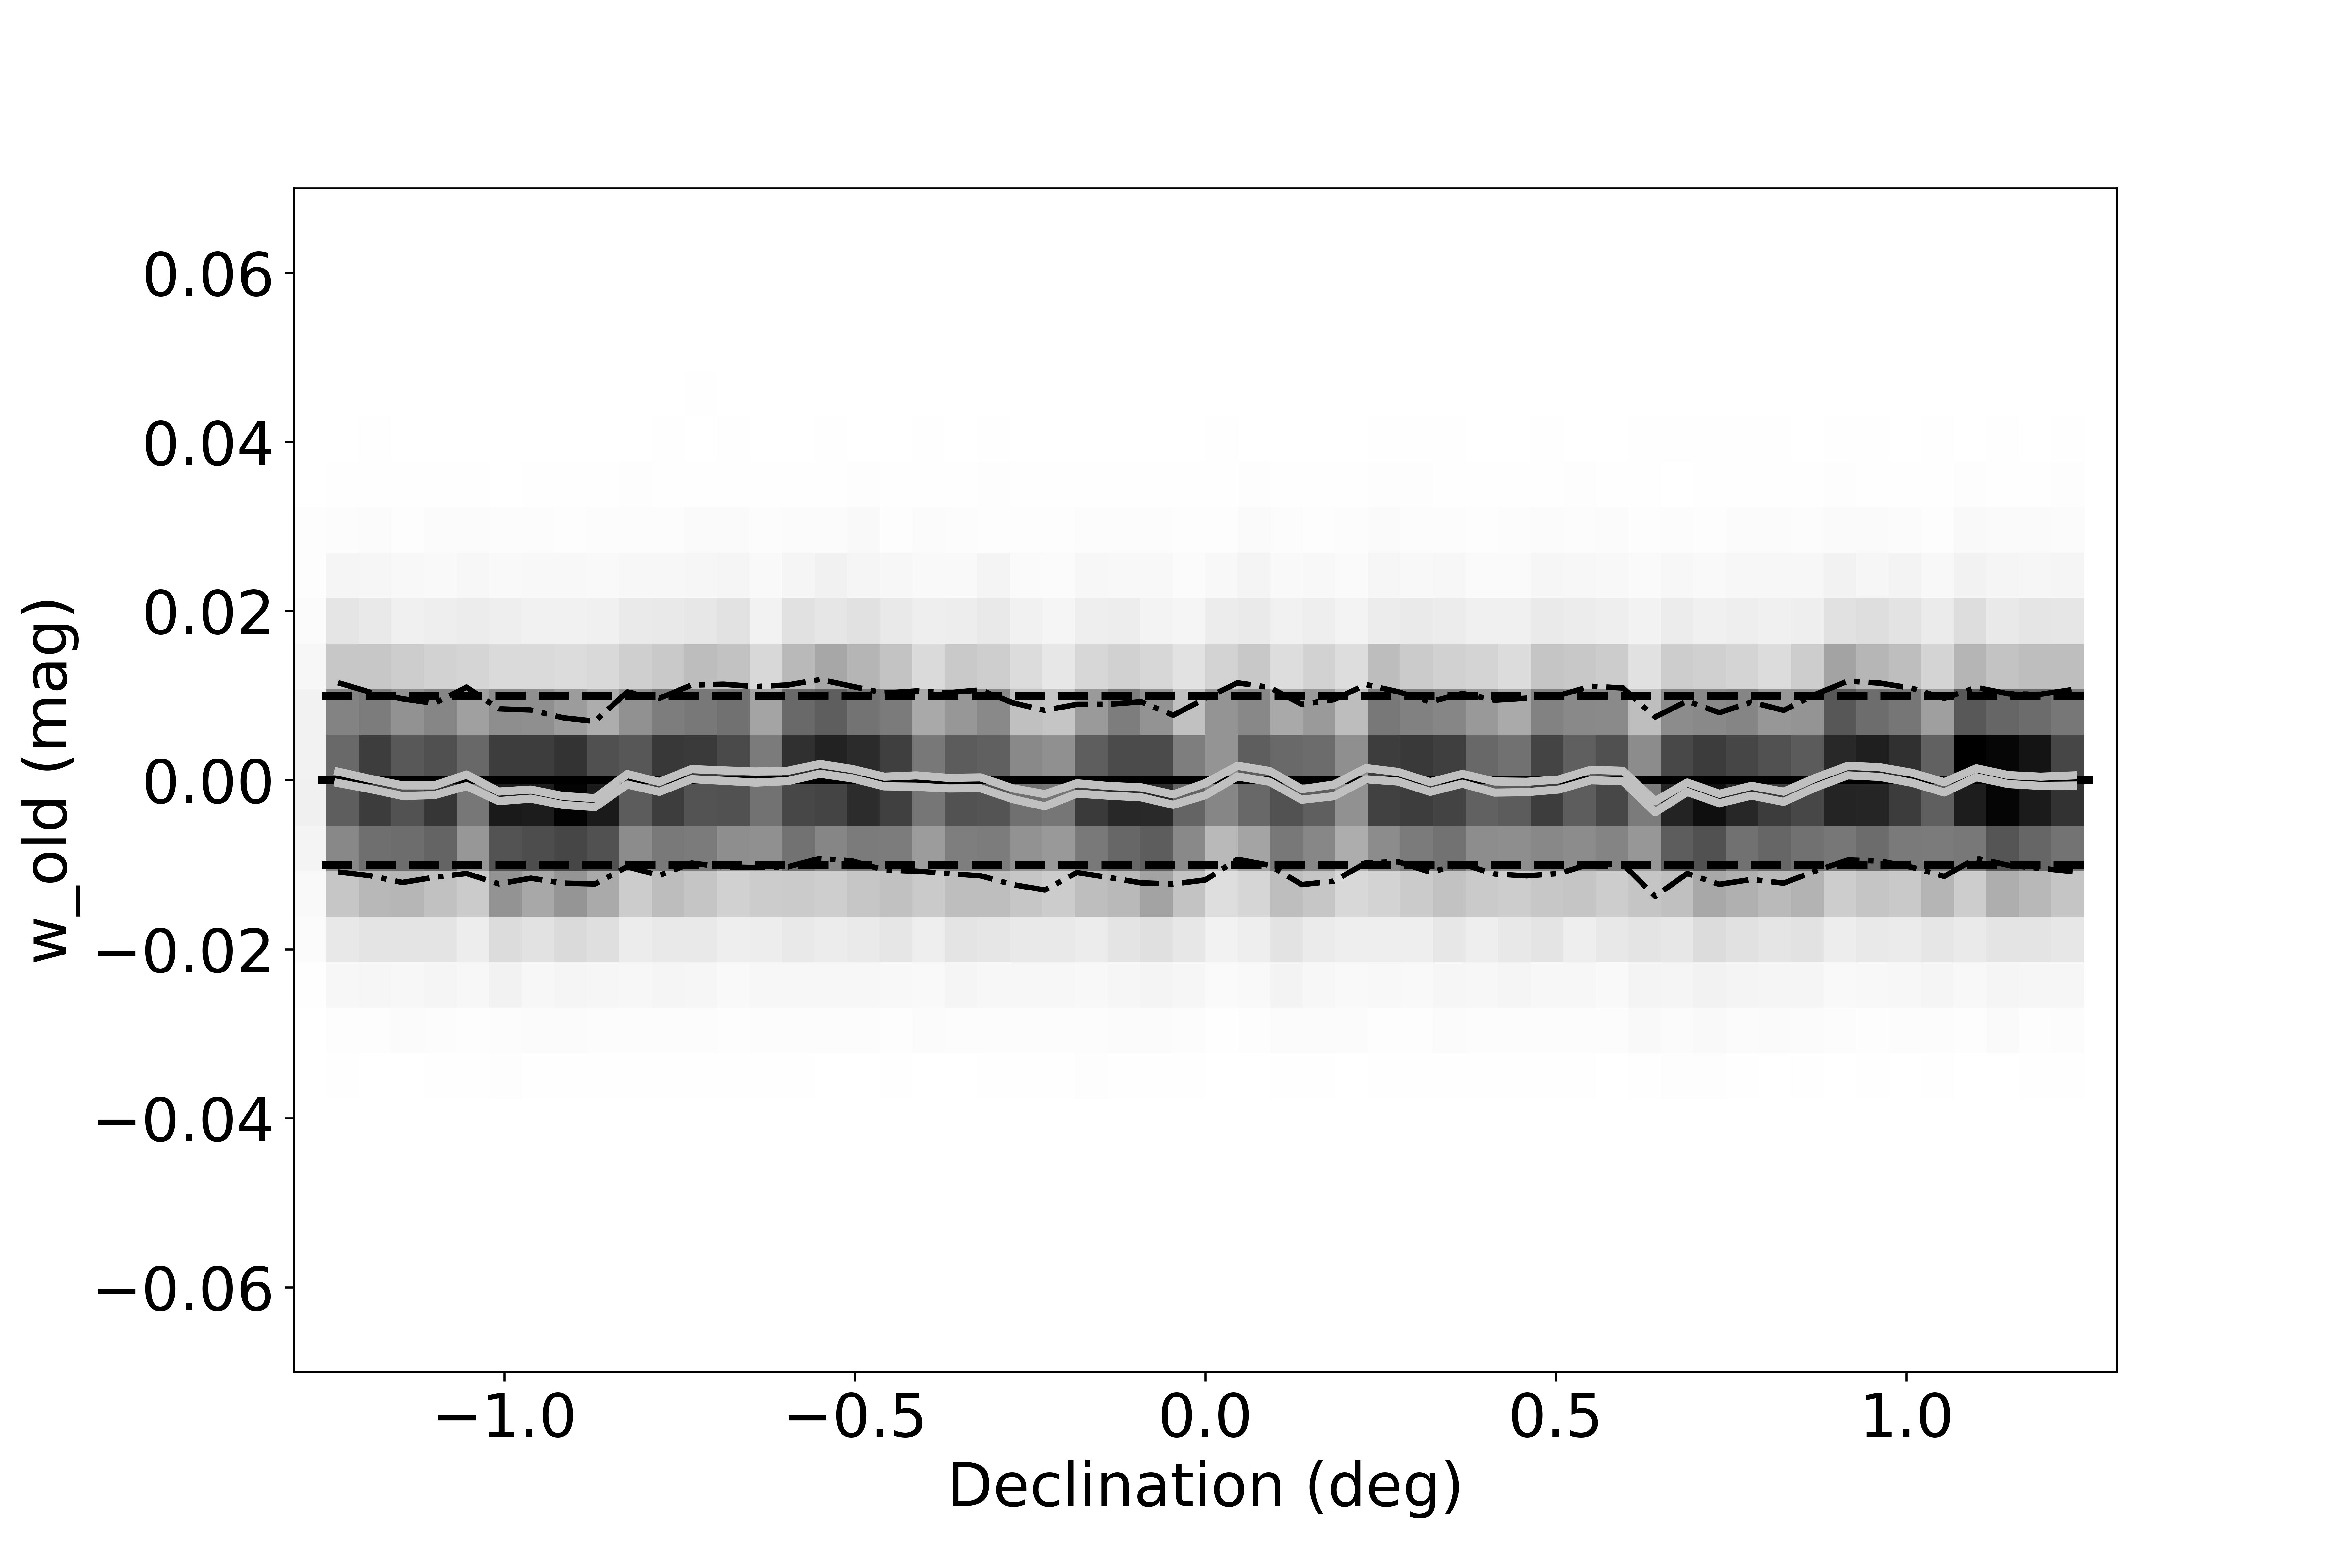
\includegraphics[width=0.45\textwidth]{figures/testV26vsV42_r_w_old_Dec_Hess.png}
    \centering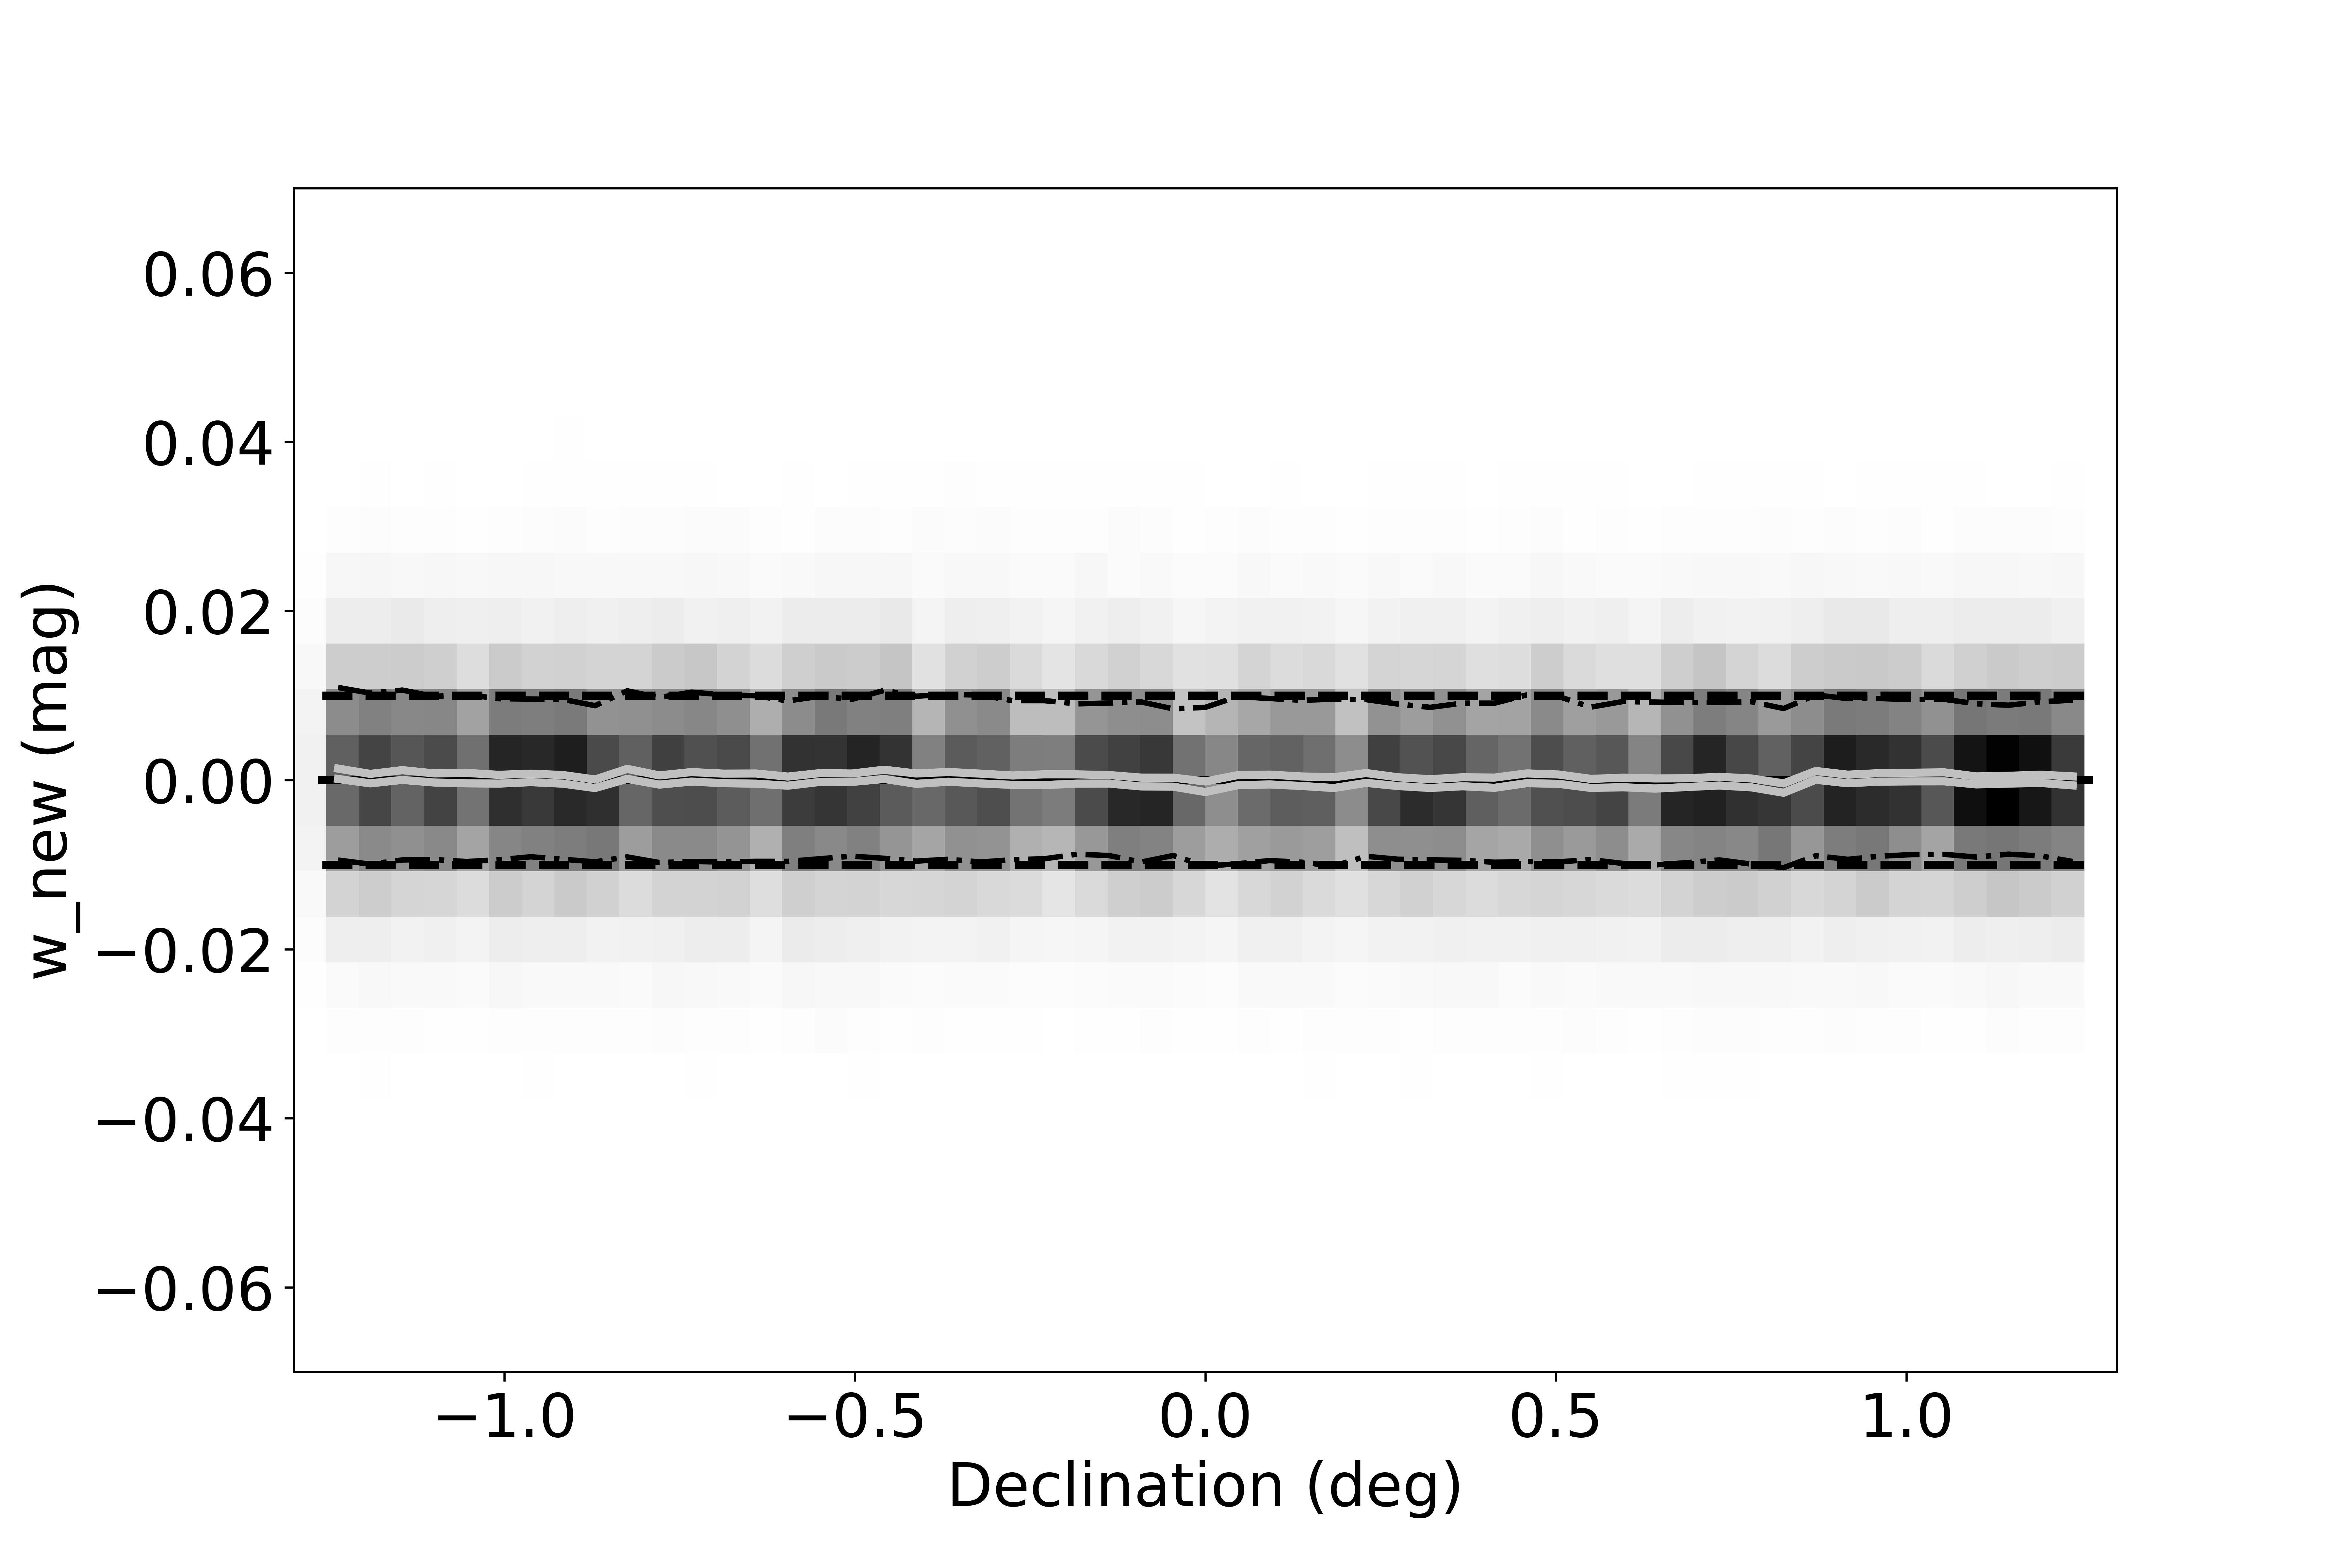
\includegraphics[width=0.45\textwidth]{figures/testV26vsV42_r_w_new_Dec_Hess.png}
\caption{A comparison of the $w$ colour, the second principal colour in the SDSS
$r-i$ vs. $g-r$ colour-colour diagram, for the v2.6 ({\it Left panels}) and v4.2 ({\it Right panels})
catalogs. The top row shows the behaviour in the R.A. direction, while the bottom row is for the Declination direction. The standard deviation of the median $w$ values binned by R.A. and Dec
is 2.6 millimag and 1.1 millimag for v2.6 and 1.0 millimag and 0.3 millimag for v4.2,
respectively.}
\label{fig:comparew} 
\end{figure*}
 

\begin{figure*}
    \centering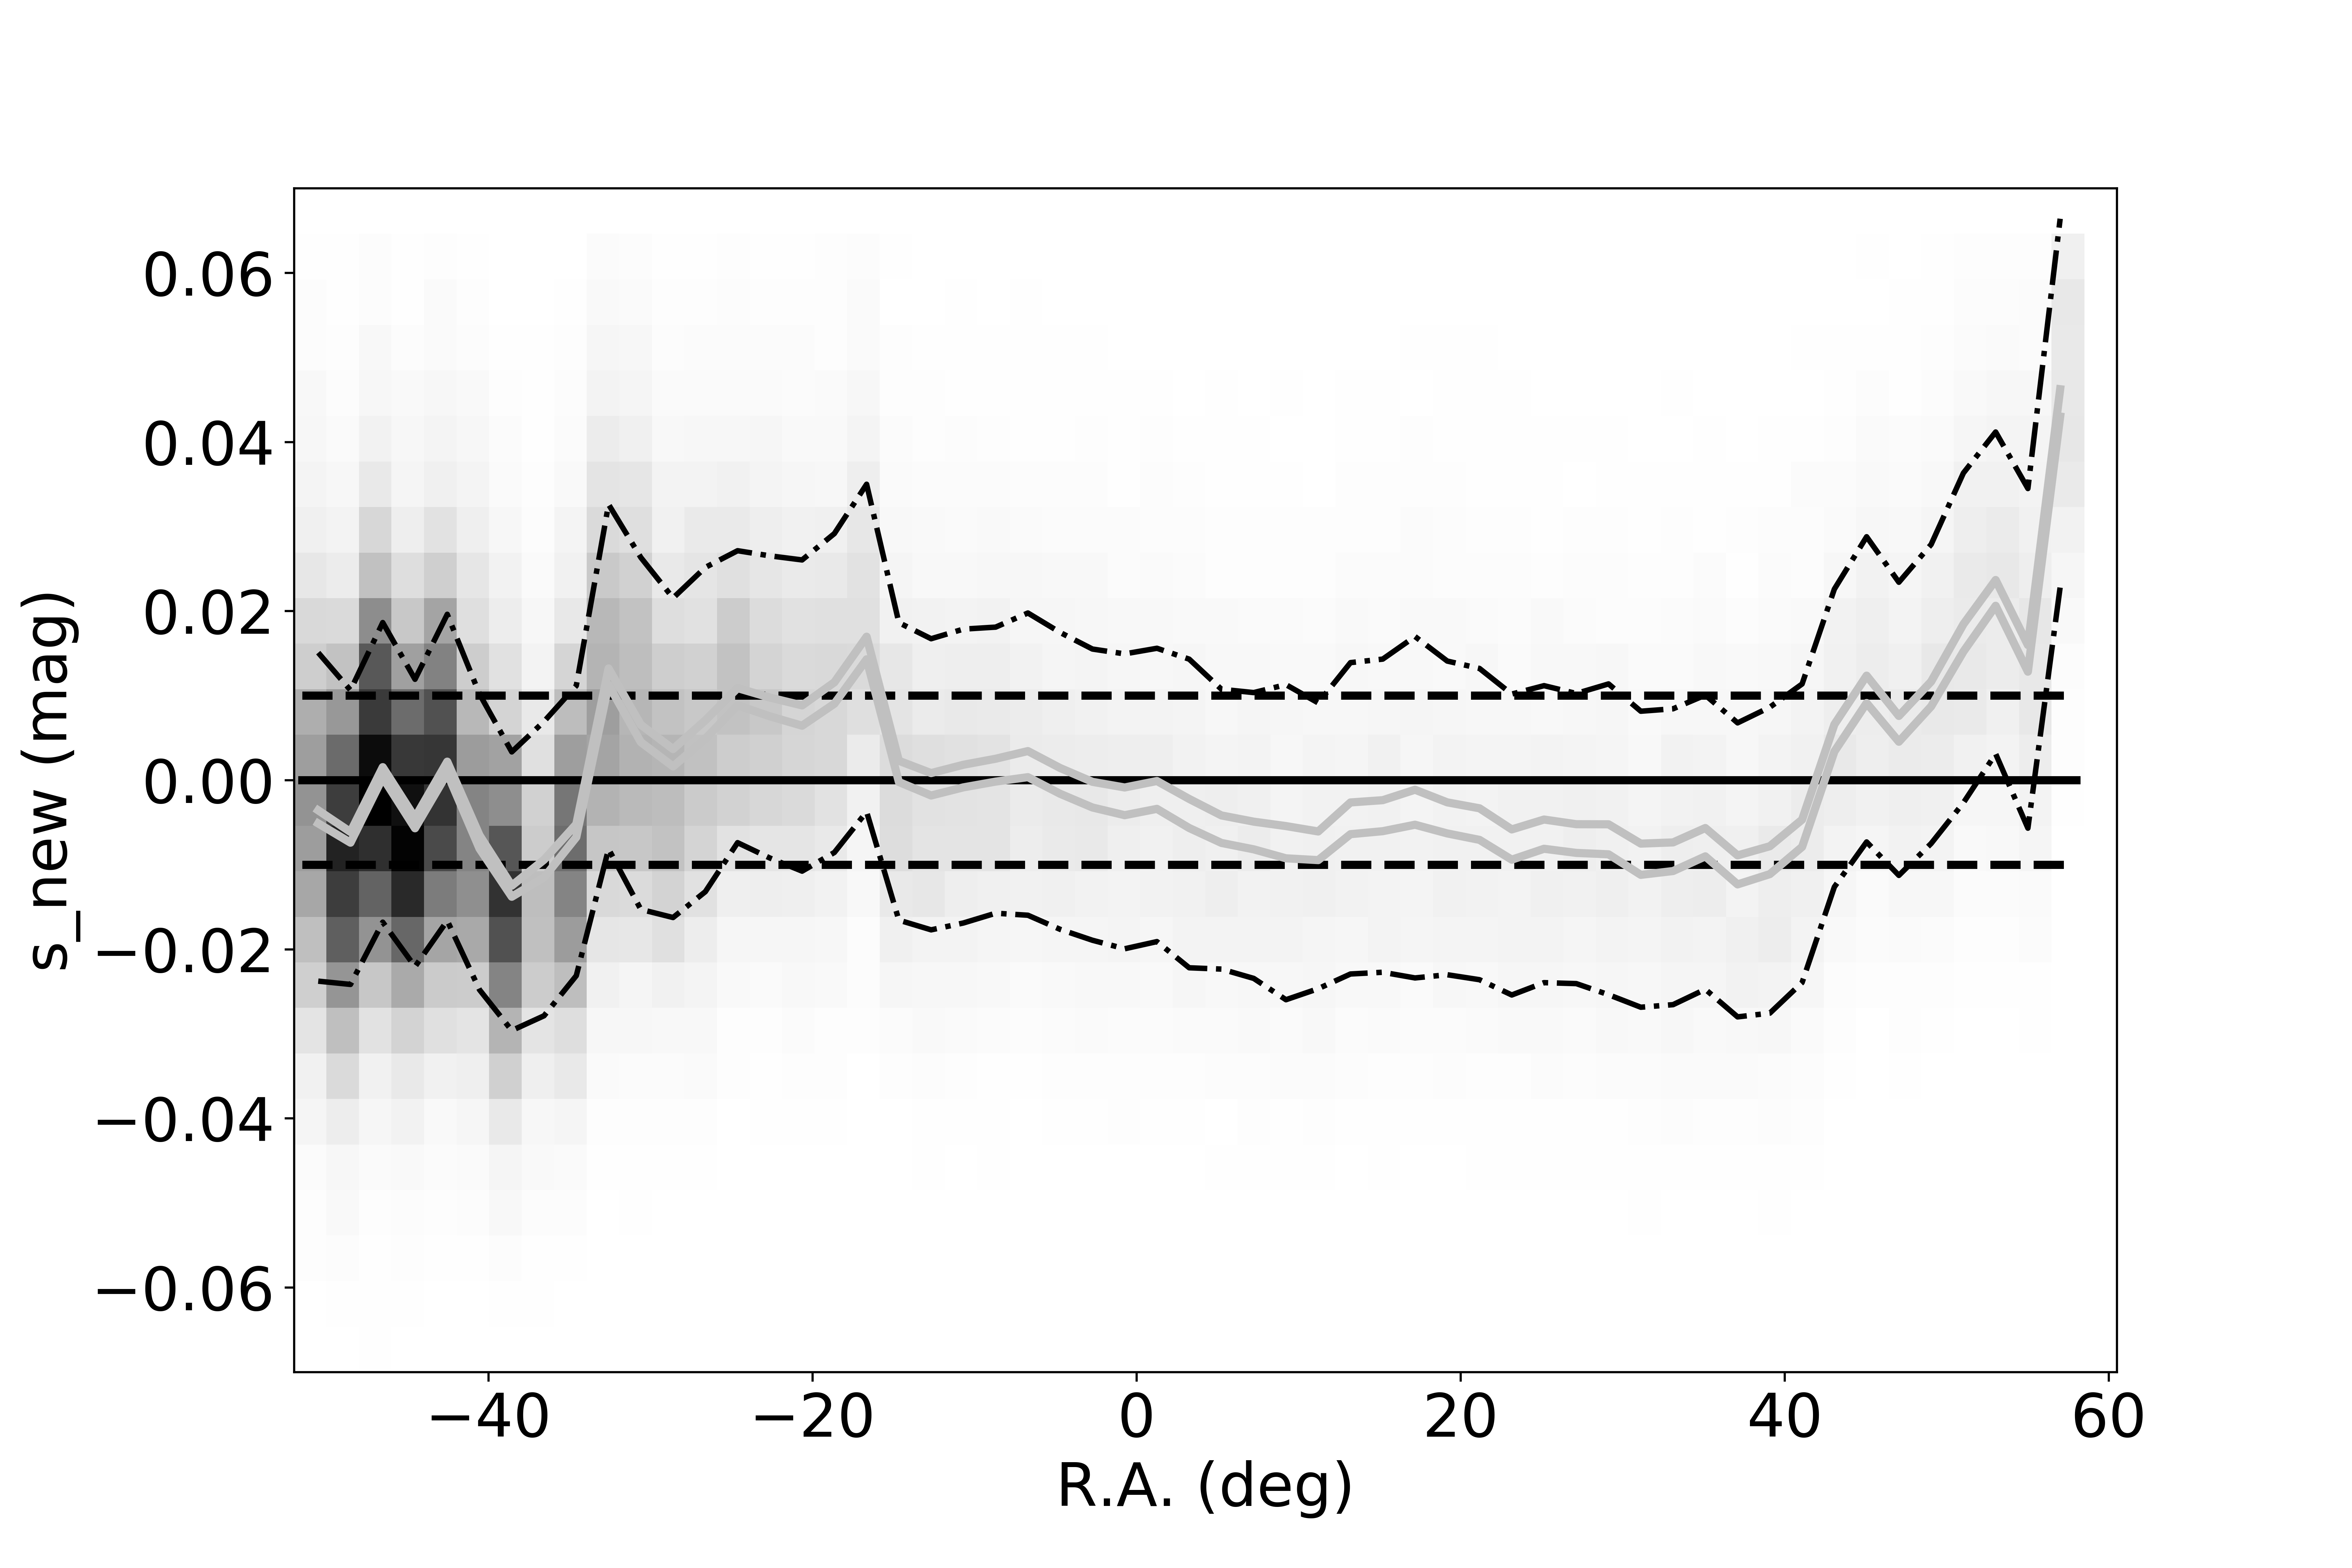
\includegraphics[width=0.45\textwidth]{figures/testV26vsV42_snew_u_s_new_RA_Hess.png}
    \centering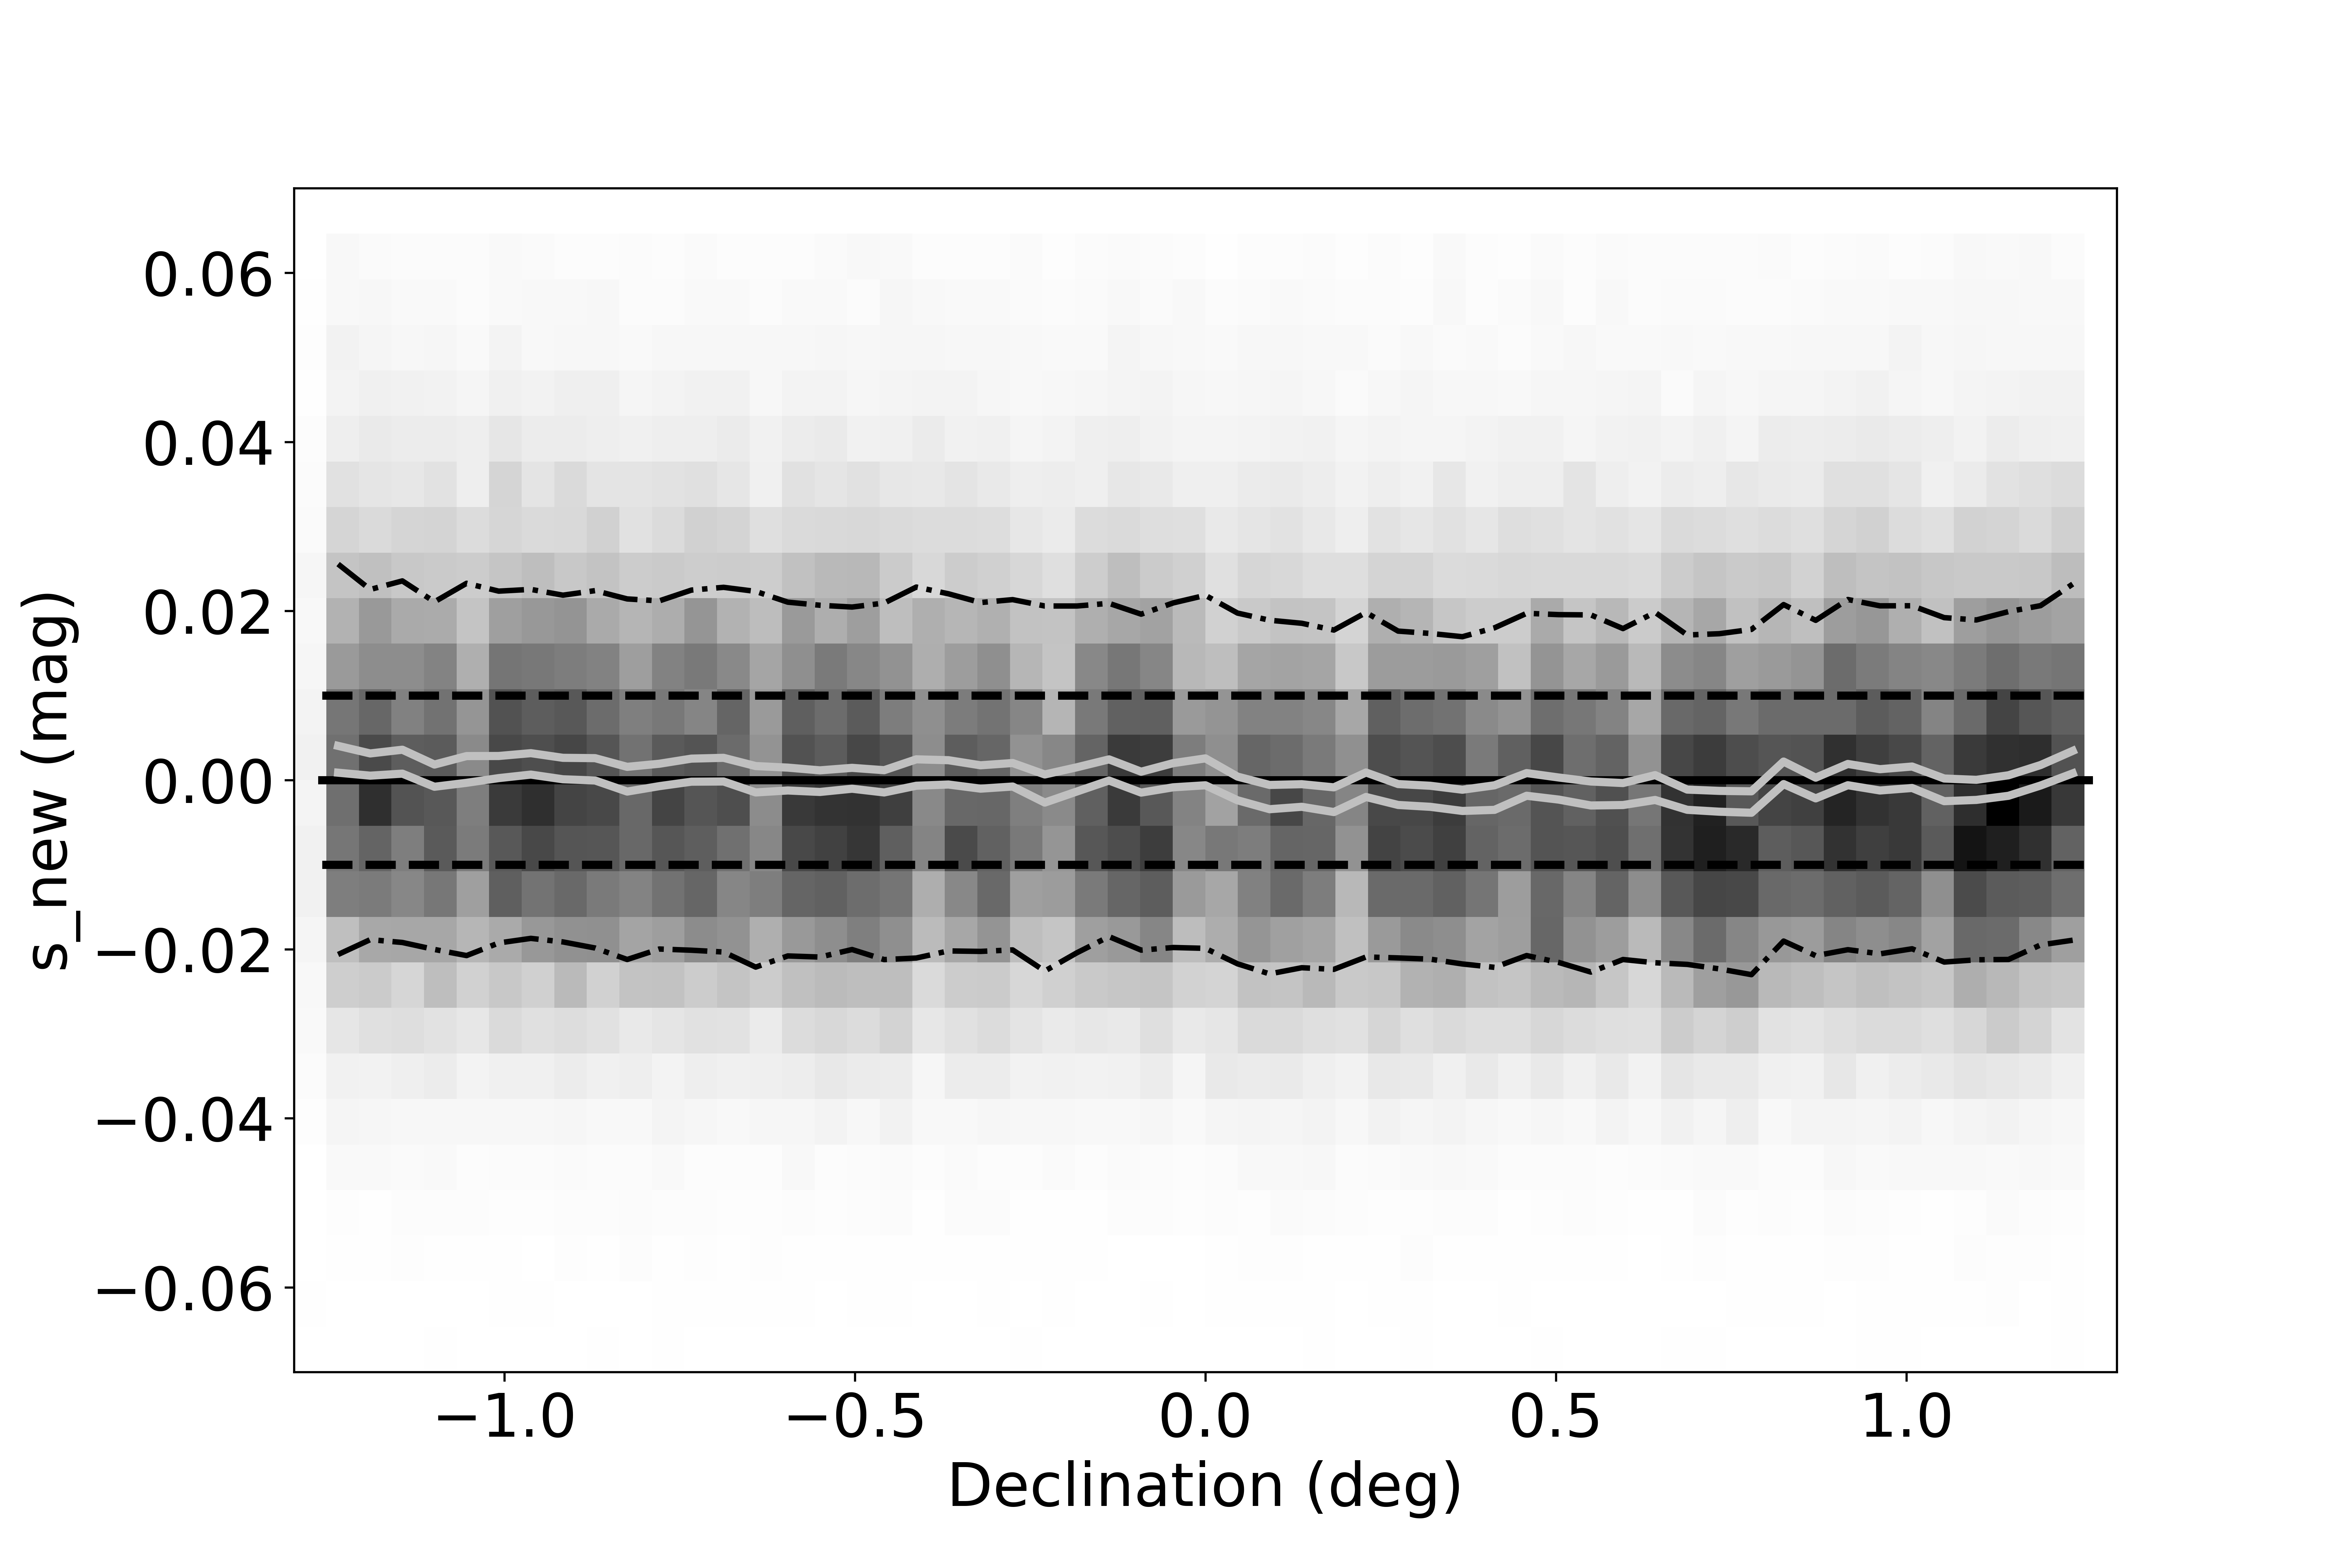
\includegraphics[width=0.45\textwidth]{figures/testV26vsV42_snew_u_s_new_Dec_Hess.png} 
    \centering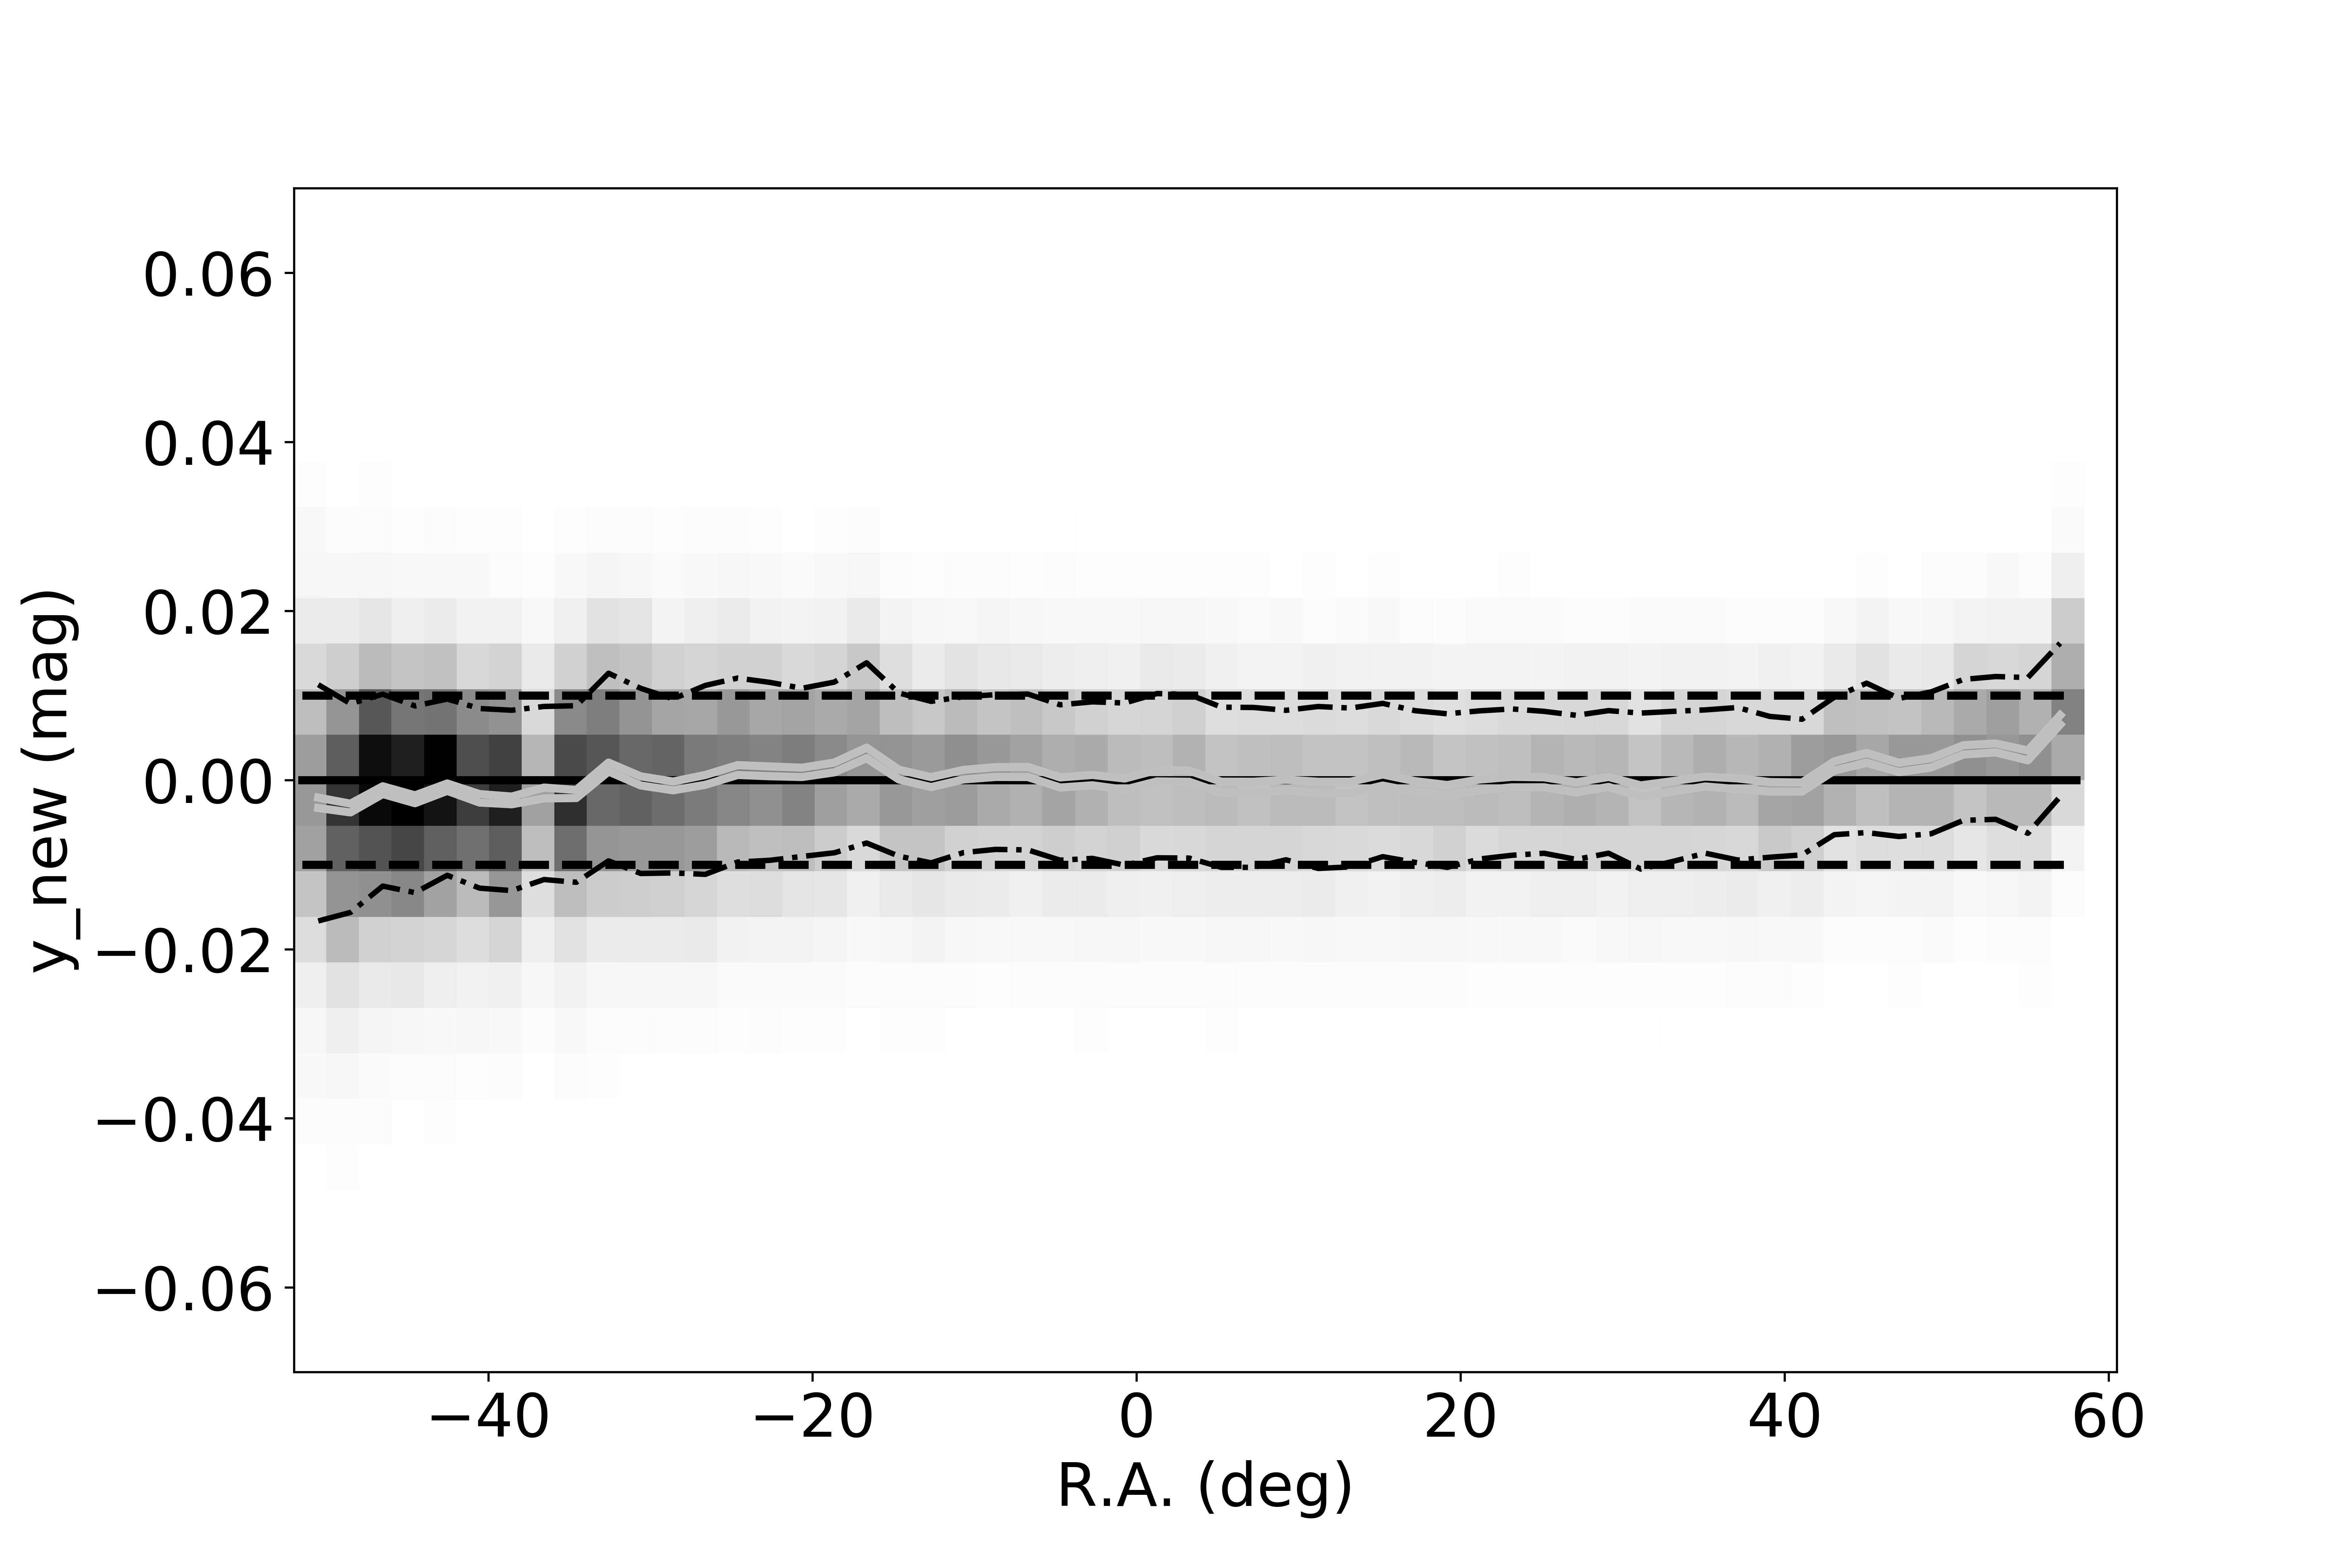
\includegraphics[width=0.45\textwidth]{figures/testV26vsV42_ynew_z_y_new_RA_Hess.png} 
    \centering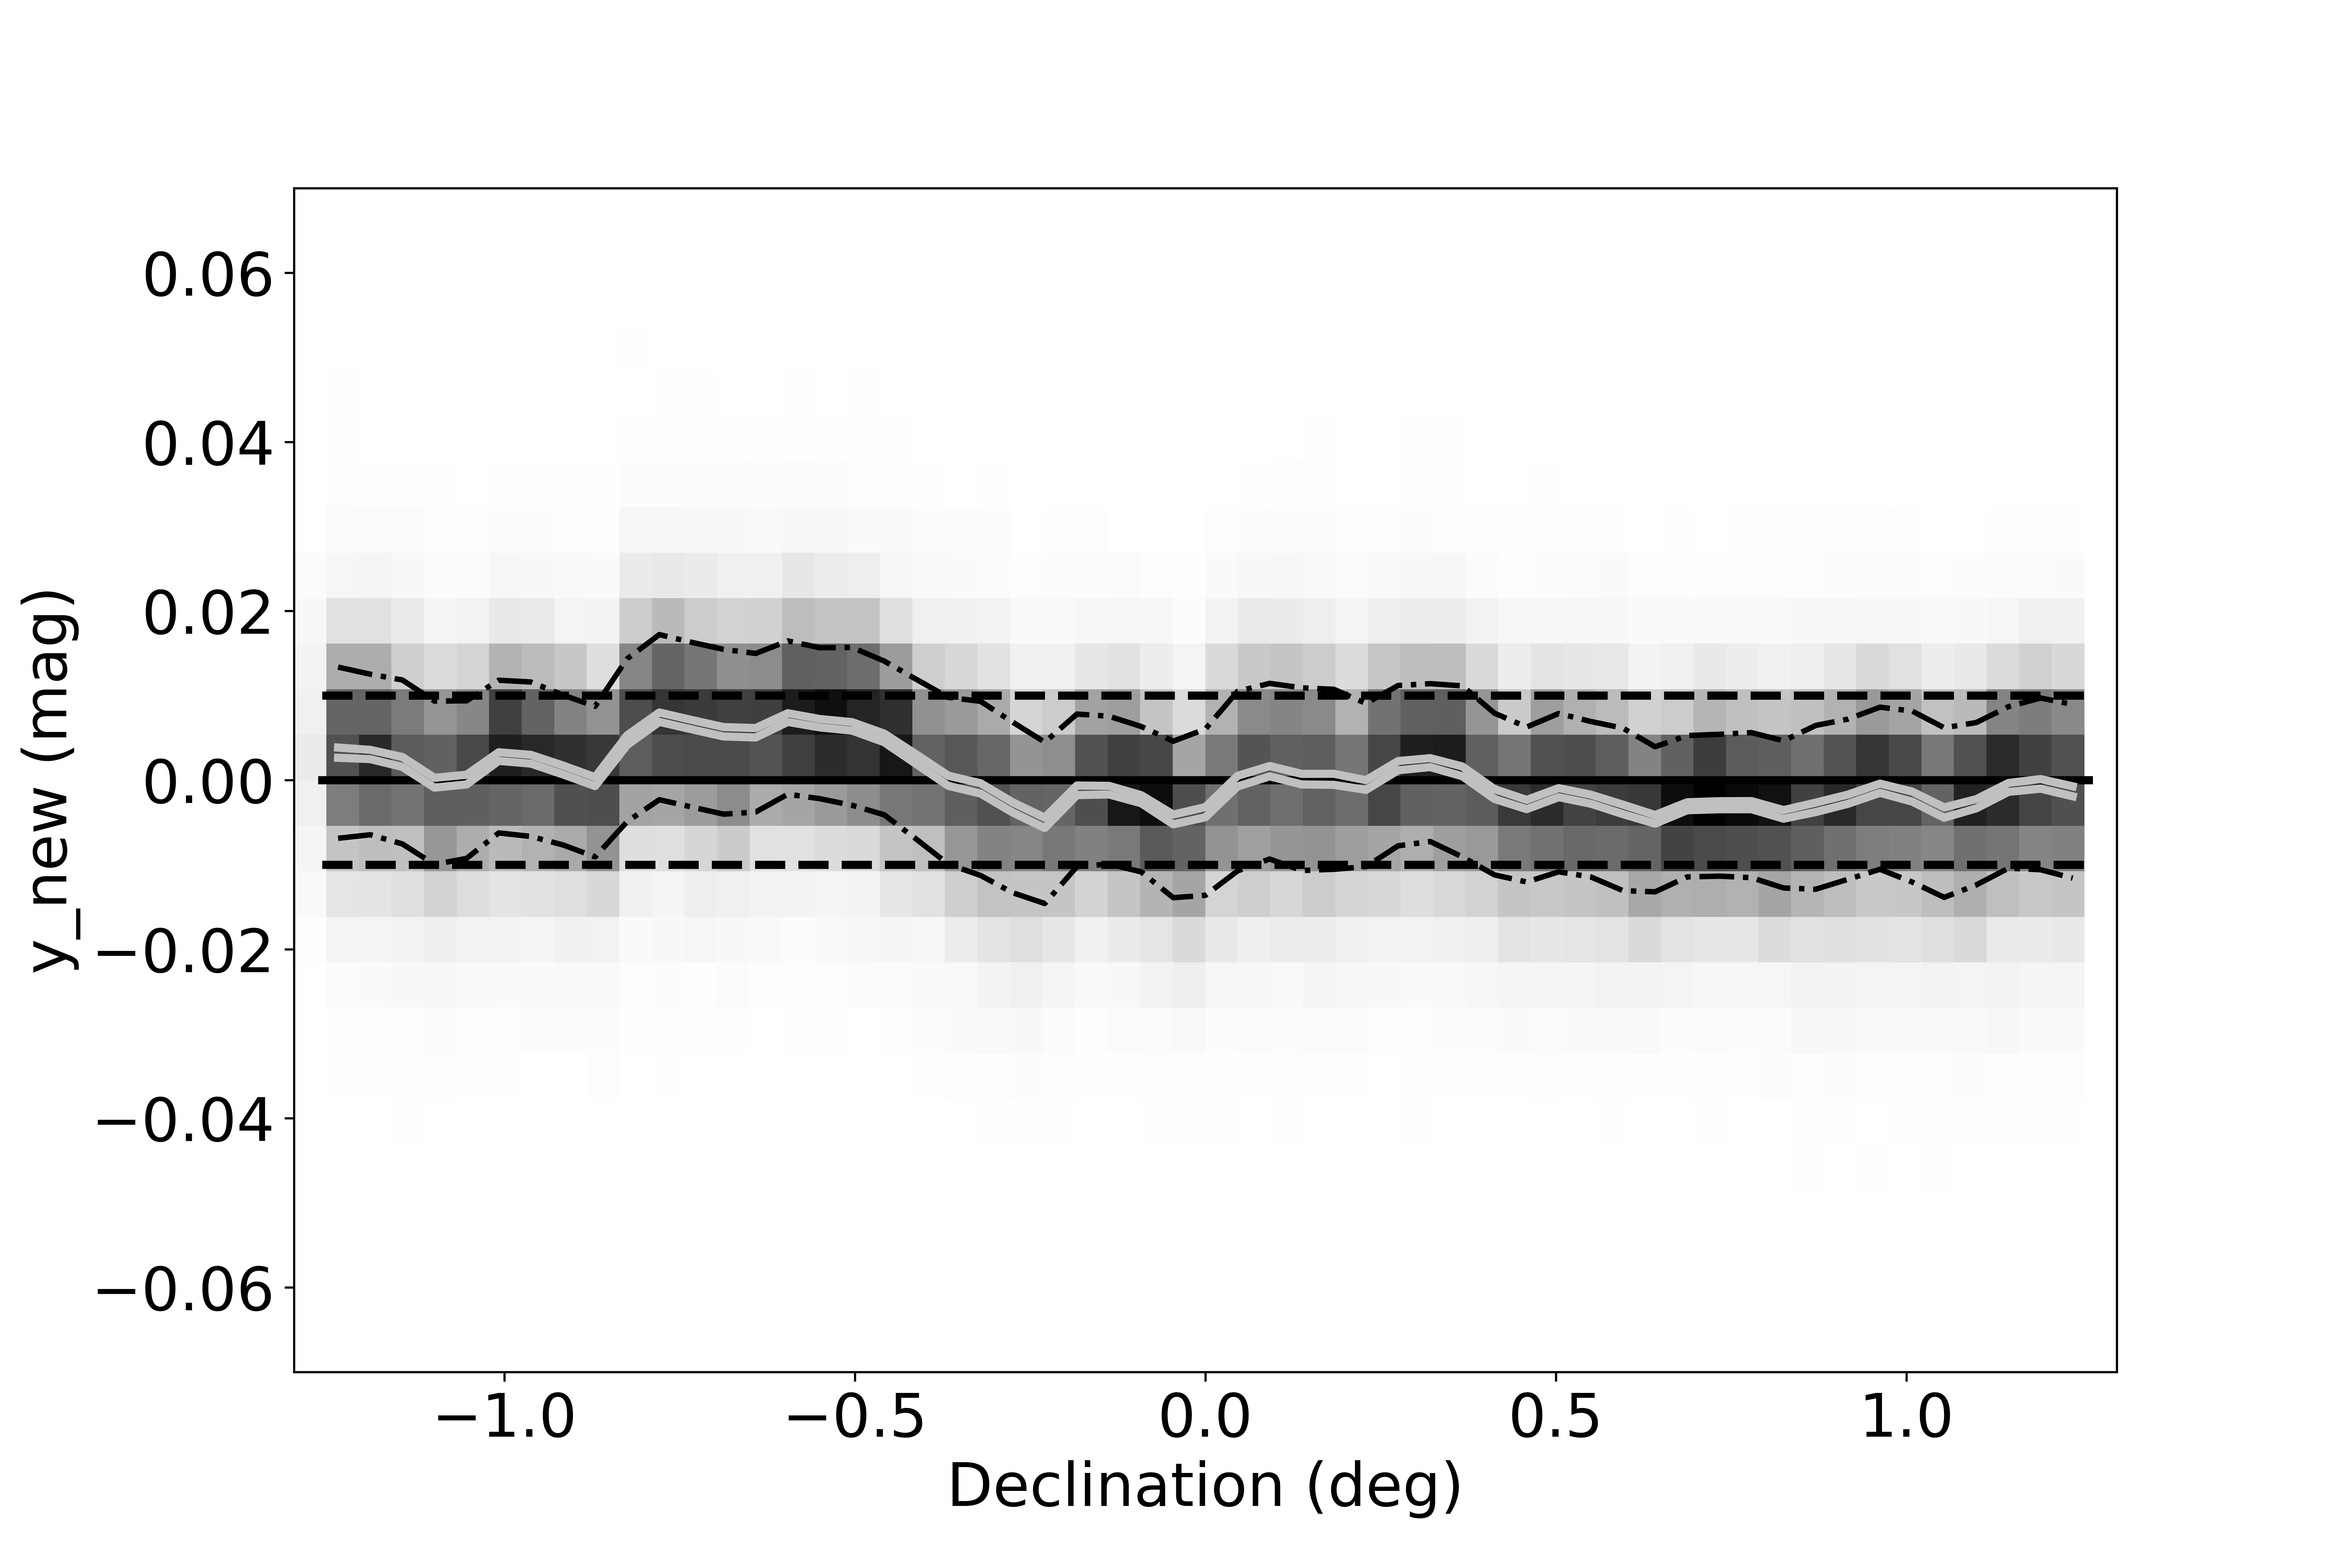
\includegraphics[width=0.45\textwidth]{figures/testV26vsV42_ynew_z_y_new_Dec_Hess.png}  
\caption{The behavior of the $s$ colour (top two panels), the second principal colour in the SDSS
$g-r$ vs. $u-g$ colour-colour diagram, and the $y$ colour (bottom two panels), the second 
principal colour in the SDSS $i-z$ vs. $r-i$ colour-colour diagram, for the new v4.2 catalog.
The standard deviation of the median $s$ values binned by R.A. and Declination is 9.8 millimag 
and 1.3 millimag, respectively, and 1.8 millimag and 3.4 millimag for the $y$ colour.}
\label{fig:comparesy} 
\end{figure*}

  
%%%%%%%%%%%%%%%%%%%%%%%%%%%%%%%%%%%%%%%%%

\subsection{Comparison of the new v4.2 SDSS catalog with DES and Pan-STARRS catalogs \label{sec:DESPS1}} 
  
The quality of photometric zeropoint calibration for the new SDSS catalog can be conveniently
tested with the DES (see Section~\ref{ssec:des}) and Pan-STARRS (see Section~\ref{ssec:ps1}) catalogs. 
Both catalogs list $griz$ photometry of sufficient precision for essentially all stars
from Stripe 82. Their photometric calibration procedures are expected to result in different 
spatial patterns and thus a cross-comparison with the v4.2 catalog can reveal residual problems
with zeropoint calibration. They are also deeper than the Gaia EDR3 catalog and thus can provide
further clues about the $\sim$0.02 mag residual Gmag gradient (bright-to-faint end bias) 
illustrated in Figure~\ref{fig:gaiaJump}. 

Our comparison of the magnitude differences is illustrated in Figures~\ref{fig:DESPSRA} and \ref{fig:DESPSDec},
and the robust standard deviation for binned median magnitude differences is listed in Table~\ref{tab:DESPS1}. 
This multi-survey comparison indicates that the spatial variation of photometric zero points in the 
updated SDSS catalog is well below 0.01 mag (RMS), with typical values of 3-7 millimag in the R.A. 
direction and 1-2 millimag in the Declination direction. Note implied DES $z$ band zeropoint errors 
as a function of R.A. of up to 0.02 mag (see the bottom left panel in Figure~\ref{fig:DESPSRA}), although a 
similar trend in the equivalent Pan-STARRS plot (bottom right panel in Figure~\ref{fig:DESPSRA}) indicates 
that the SDSS catalog, calibrated using Gaia EDR3, may be at least partially responsible for observed 
differences\footnote{For a comparison of DES DR1 and Gaia DR2 calibrations, see e.g., Fig. 9 of \citet{2018ApJS..239...18A}}

The variation of the residual magnitude differences with magnitude (see Figure~\ref{fig:drVSr} for DES results) 
is typically flat to within $\sim$3-4 millimag for both DES and Pan-STARRS. This much smaller gradient than observed 
for Gaia ($\sim$20 millimag) implies a likely problem (a bias between bright and faint ends) with Gaia EDR3 
photometry. The largest discrepancy of about 2 millimag/mag is observed for the Pan-STARRS $r$ band, 
while when comparing to DES $r$ band, the gradient is limited to $<$1 millimag. 

% \begin{deluxetable}{l|c|c|c|c}[ht!]
% \tablecaption{The robust standard deviation for binned median magnitude differences between
% the new v4.2 SDSS catalog, and DES and Pan-STARRS1 (PS1) catalogs (millimag). \label{tab:DESPS1}}
% \tablehead{
% \colhead{Band} & \colhead{DES R.A.} & \colhead{DES Dec} & \colhead{PS1 R.A.} & \colhead{PS1 Dec} 
% }
% \startdata
% THESE ARE OLD VALUES FOR v4.2 catalog
%        $g$        &        5.1    &      1.8   &        3.4    &      1.4        \\
%        $r$         &        4.1    &      0.8   &        2.6    &      0.7         \\  
%        $i$         &        7.3    &      1.6   &        3.2    &      1.0         \\ 
%        $z$        &       13.6    &     3.6   &        6.8    &      2.3         \\ 
% \enddata
% \end{deluxetable}
   
\begin{table}
	\centering
	\caption{The robust standard deviation for binned median magnitude differences between
the new v4.2 SDSS catalog, and DES and Pan-STARRS1 catalogs (millimag).}
	\label{tab:DESPS1}
	\begin{tabular}{l|c|c|c|c} % 
		\hline
		Band & DES R.A. & DES Dec. & PS1 R.A. & PS1 Dec. \\
		\hline
% updated by ZI for v4.2
       $g$        &        4.8    &      2.0   &        3.3    &      1.6        \\
       $r$         &        3.3    &      0.9   &        2.1    &      0.9         \\  
       $i$         &        5.9    &      1.4   &        2.2    &      1.0         \\ 
       $z$        &       12.1    &     3.6   &        5.1    &      2.3         \\ 
		\hline
	\end{tabular}
\end{table}


\begin{figure*}
    \centering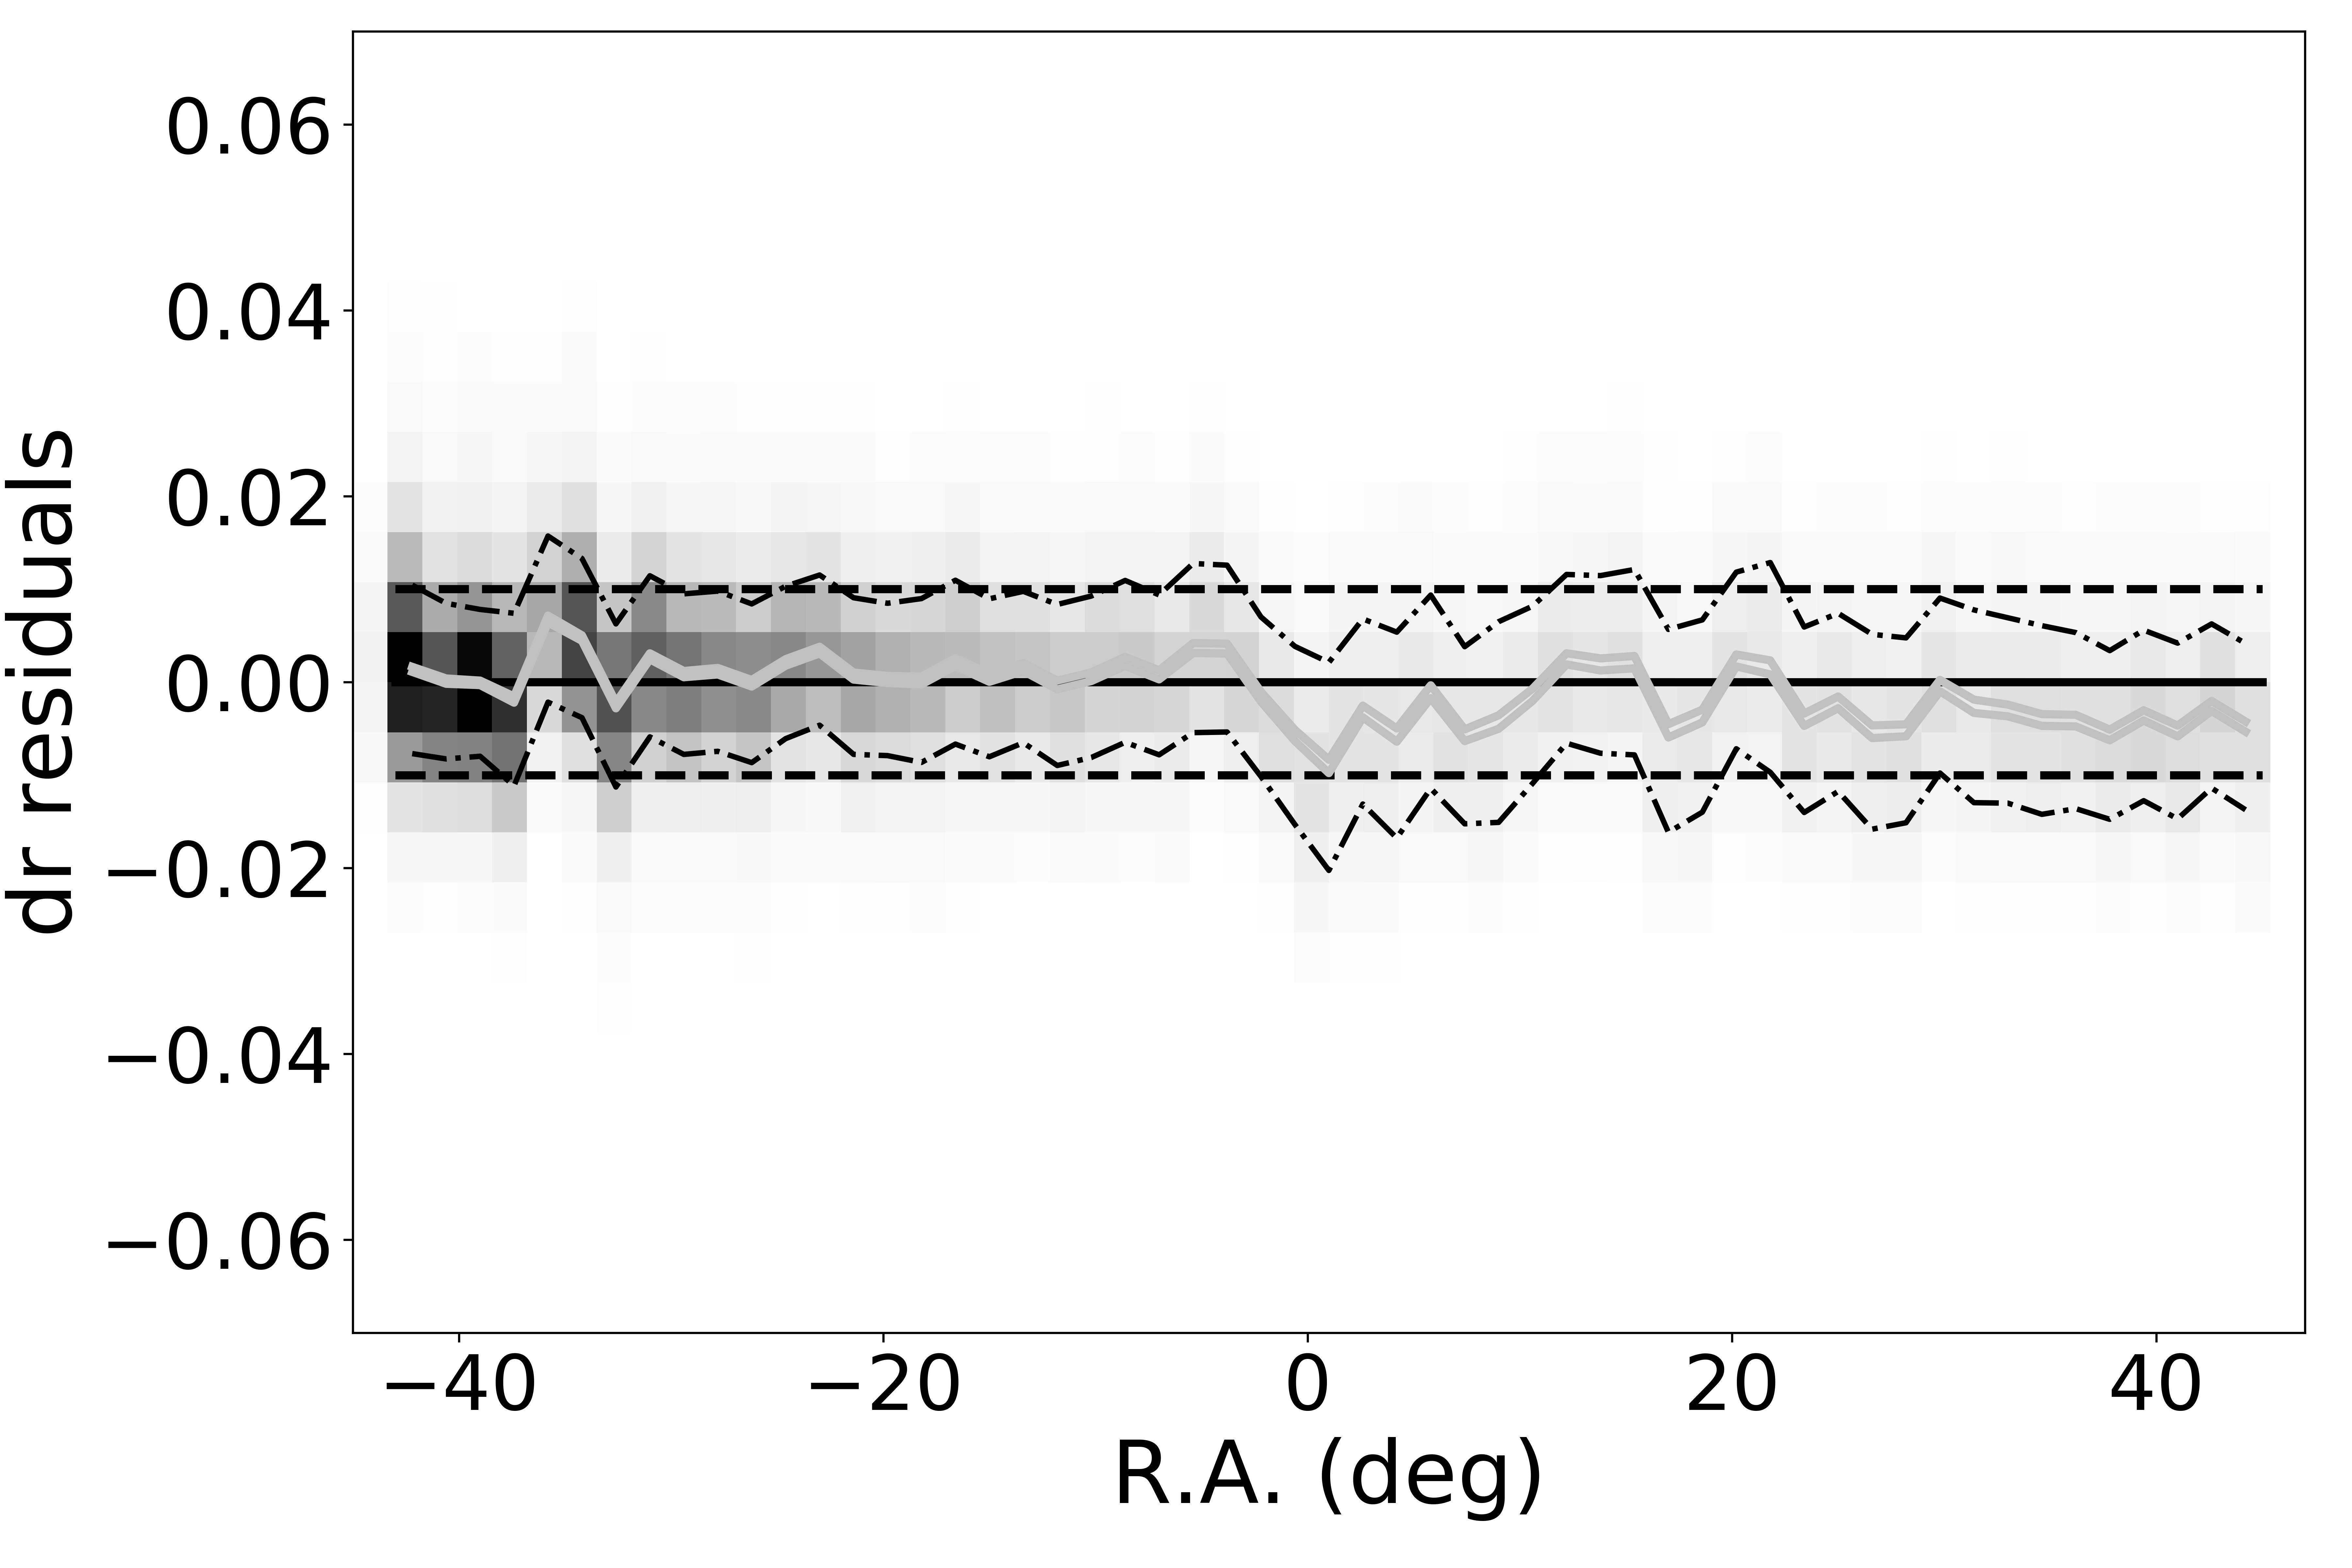
\includegraphics[width=0.45\textwidth]{figures/colorResidDES42bright_dr_RA_Hess.png}
    % \centering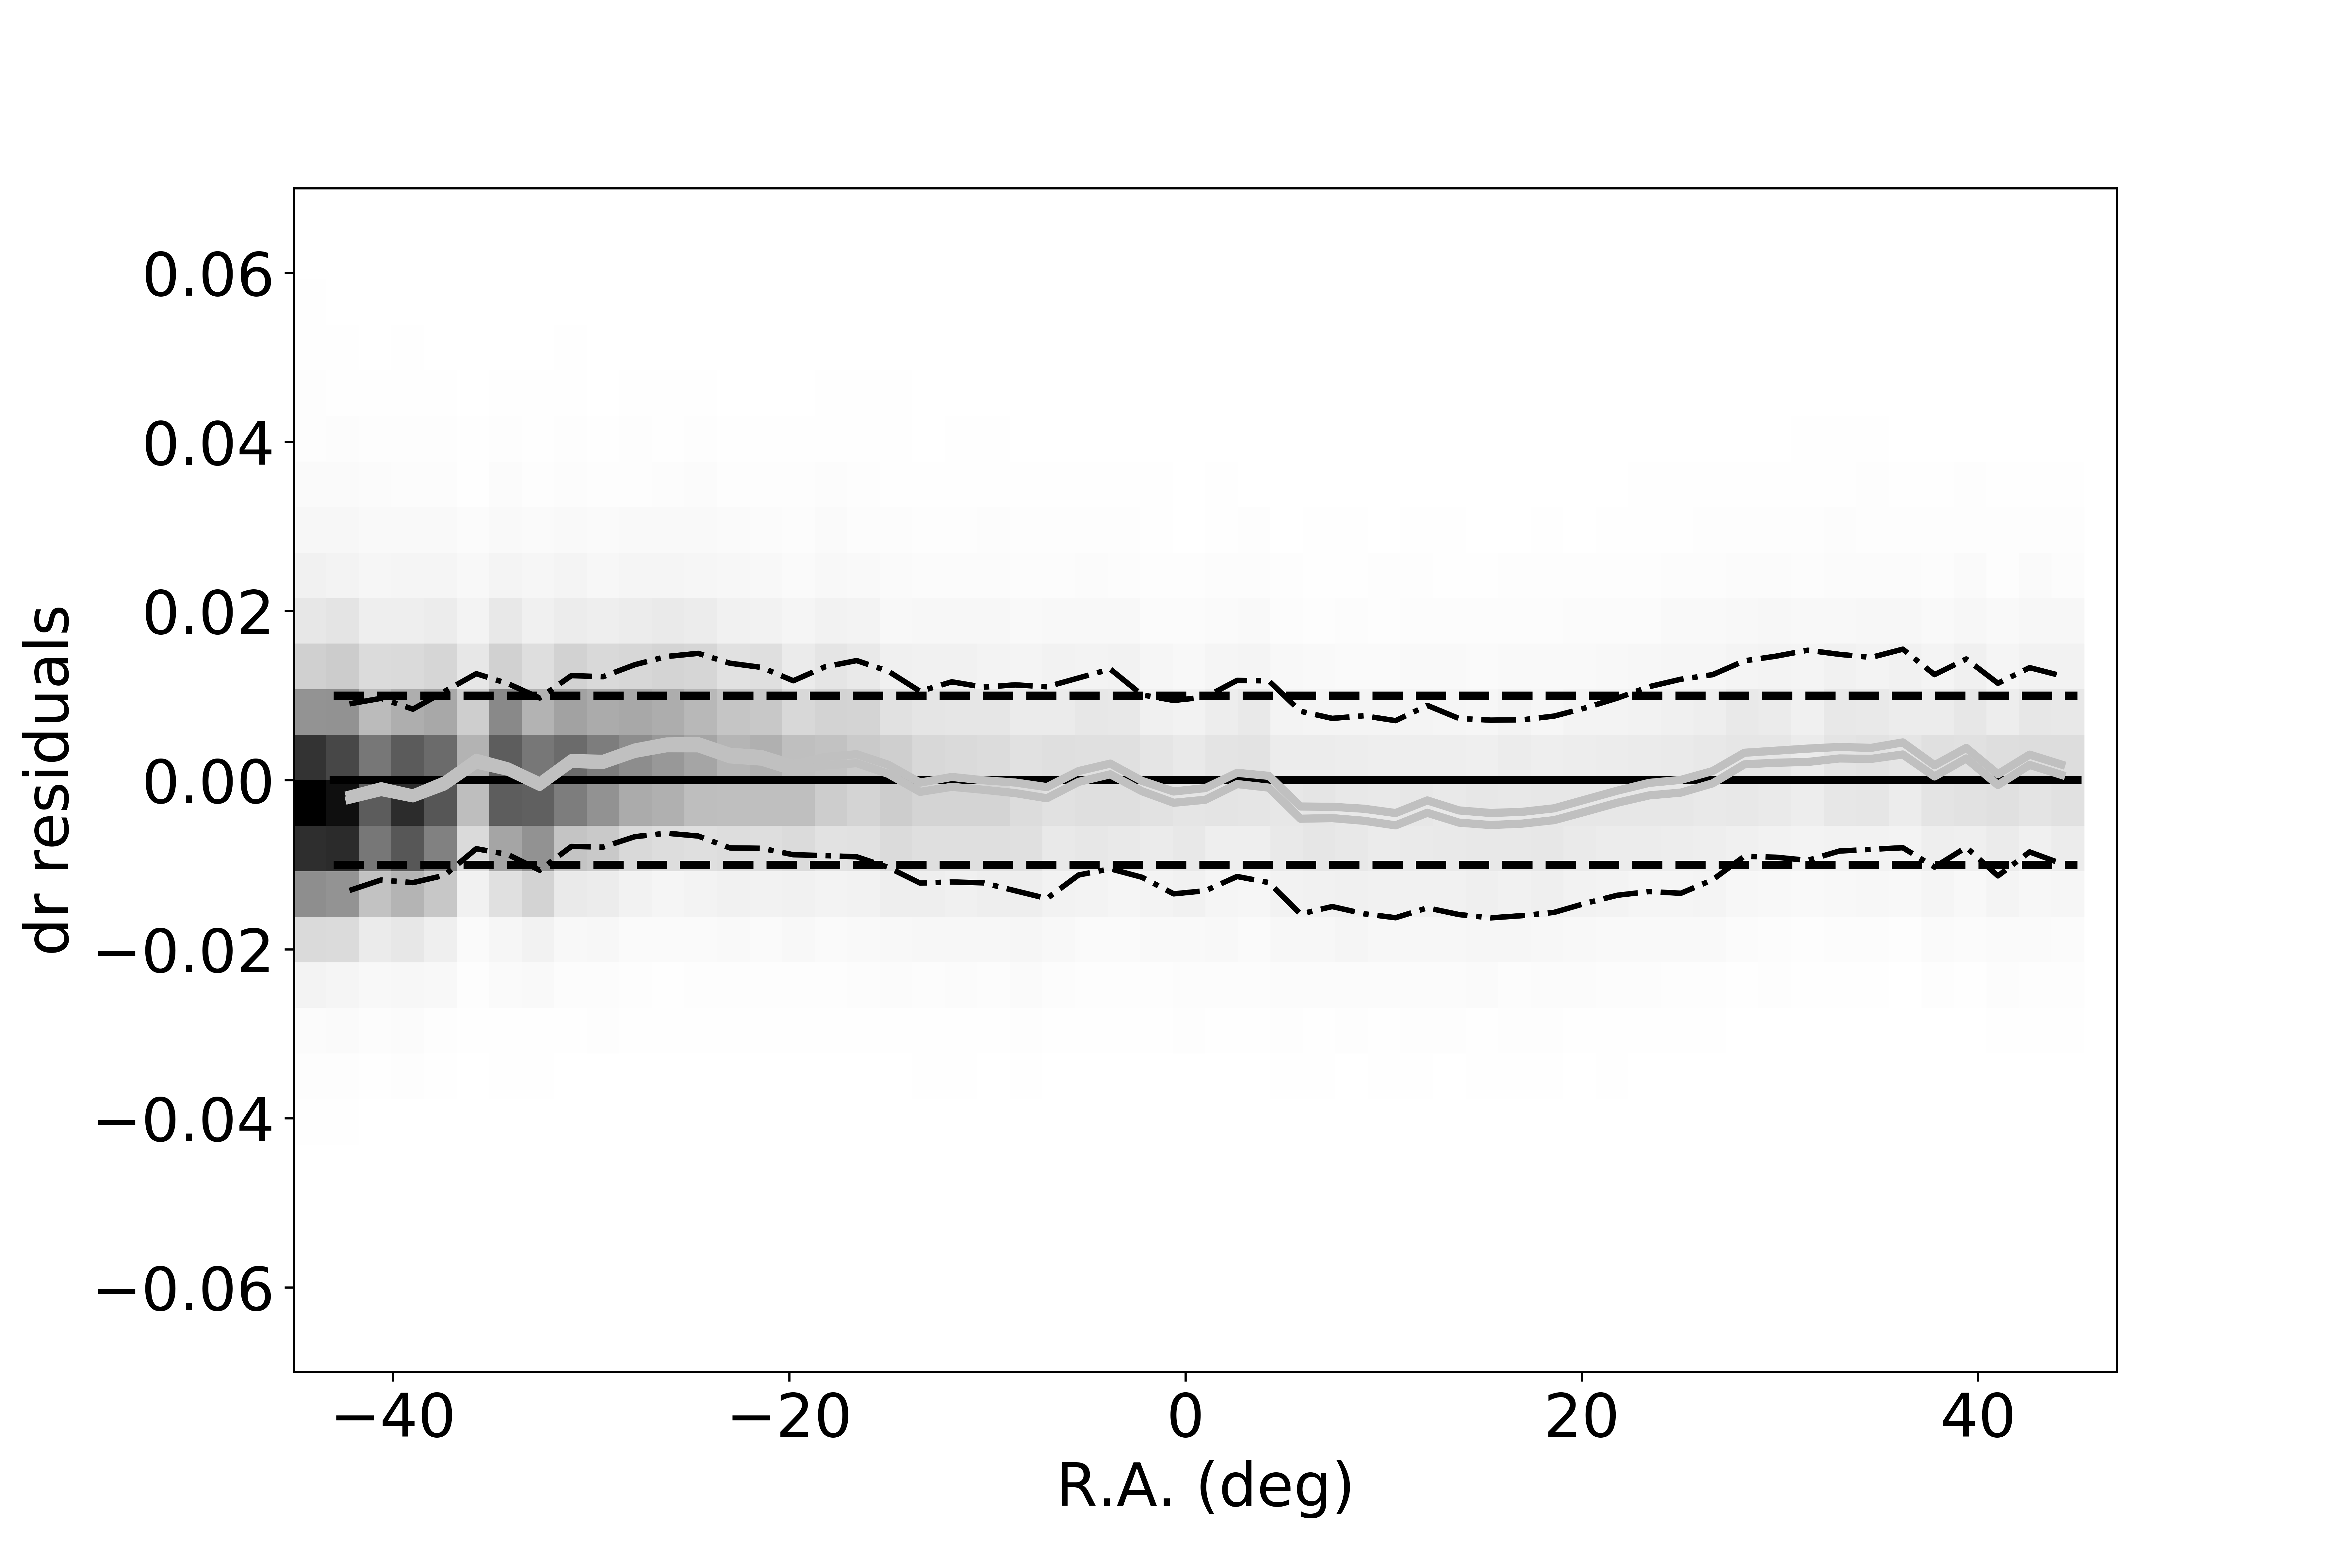
\includegraphics[width=0.45\textwidth]{figures/colorResidPSbright_dr_RA_Hess.png}
    \centering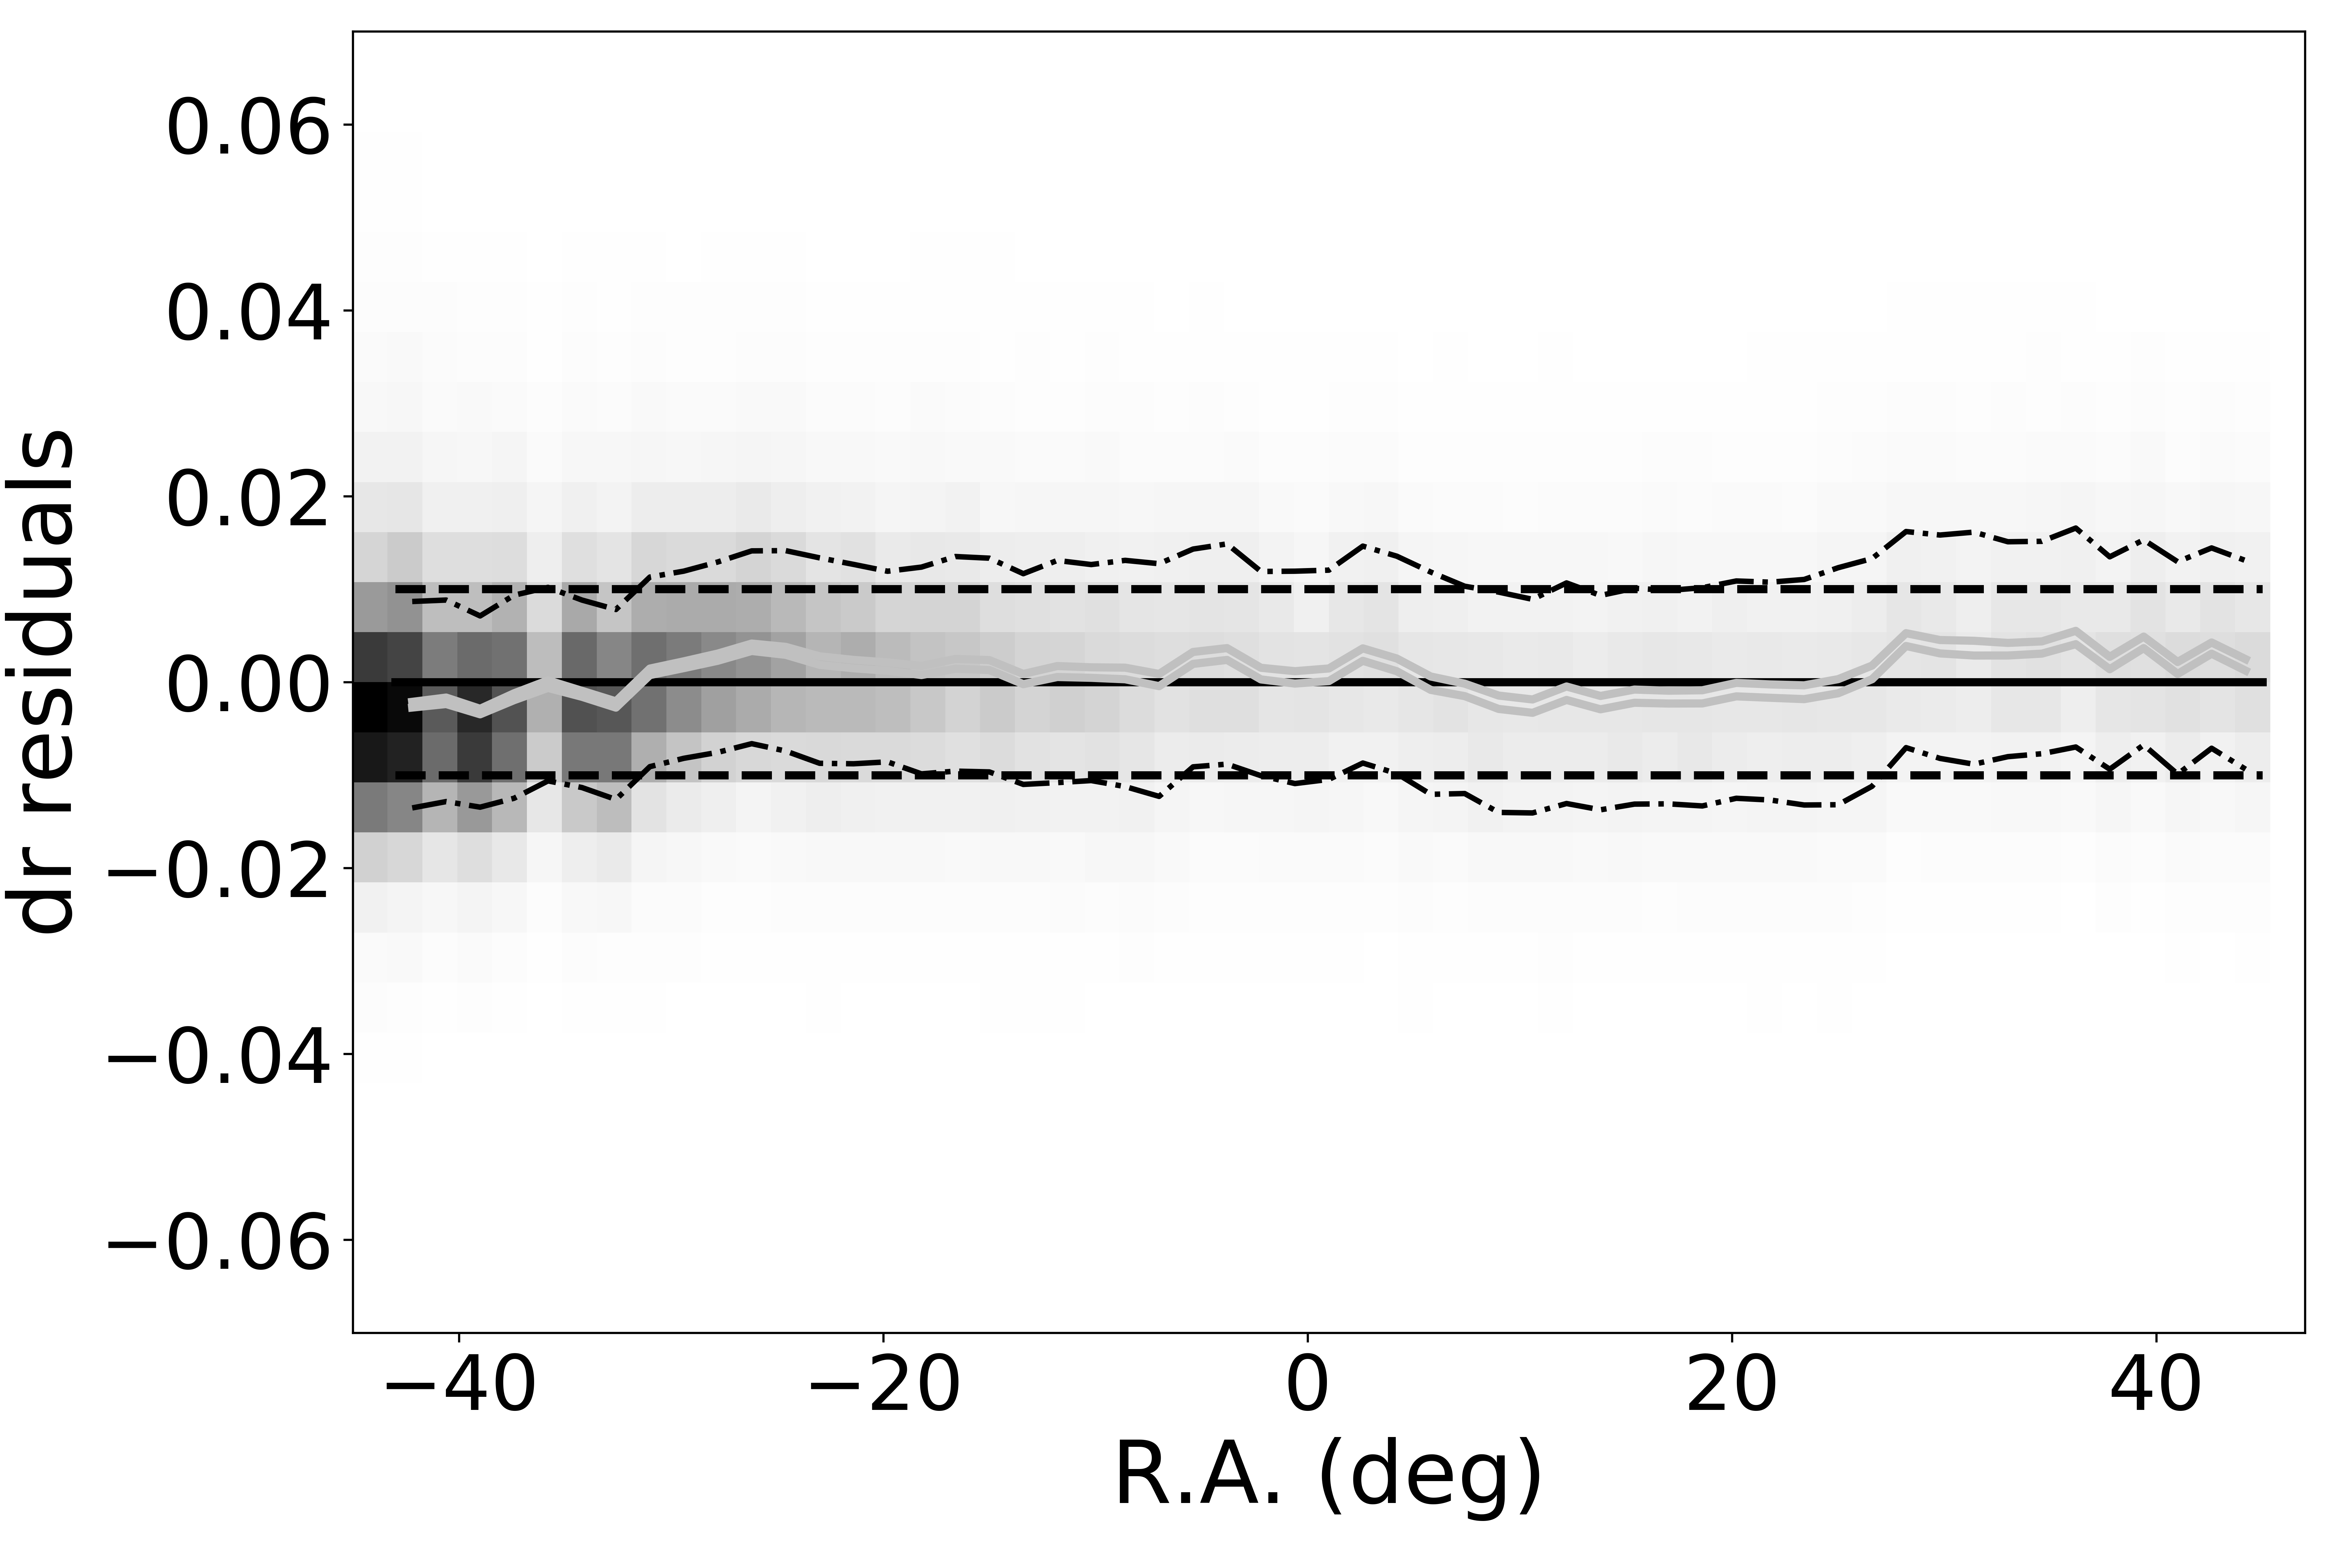
\includegraphics[width=0.45\textwidth]{figures/colorResidPSDR2v42bright_dr_RA_Hess.png}
    \centering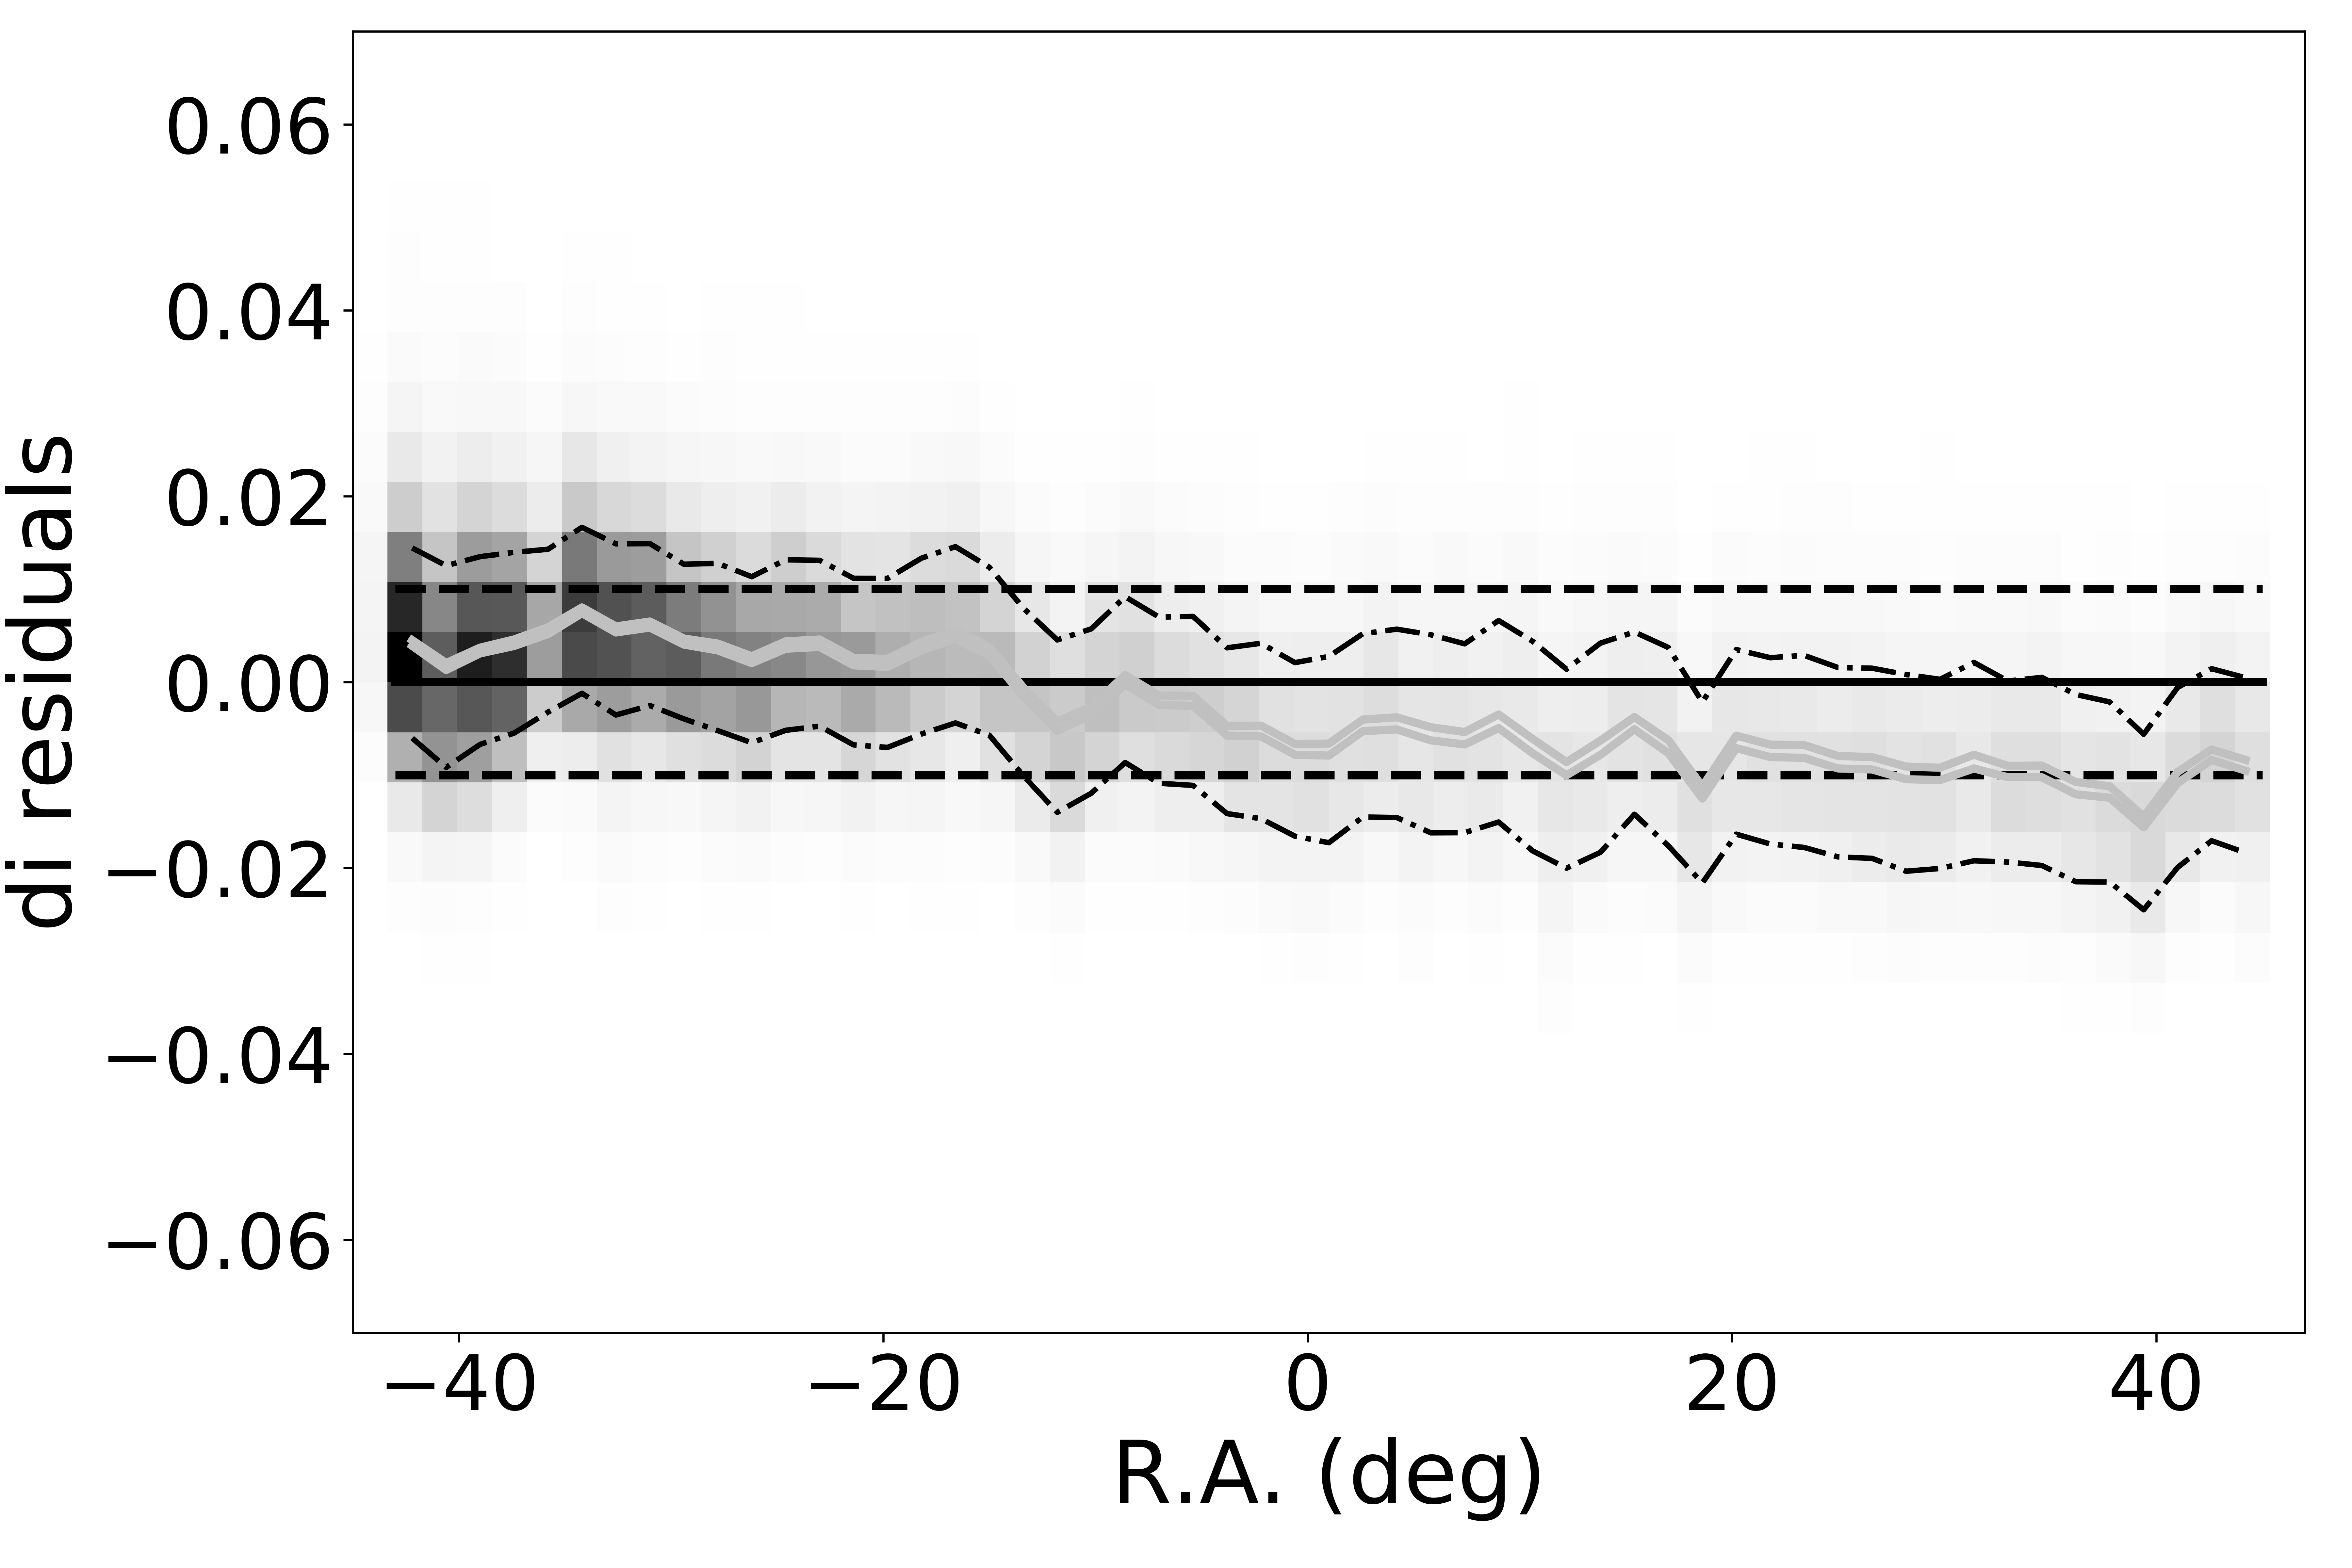
\includegraphics[width=0.45\textwidth]{figures/colorResidDES42bright_di_RA_Hess.png}
    % \centering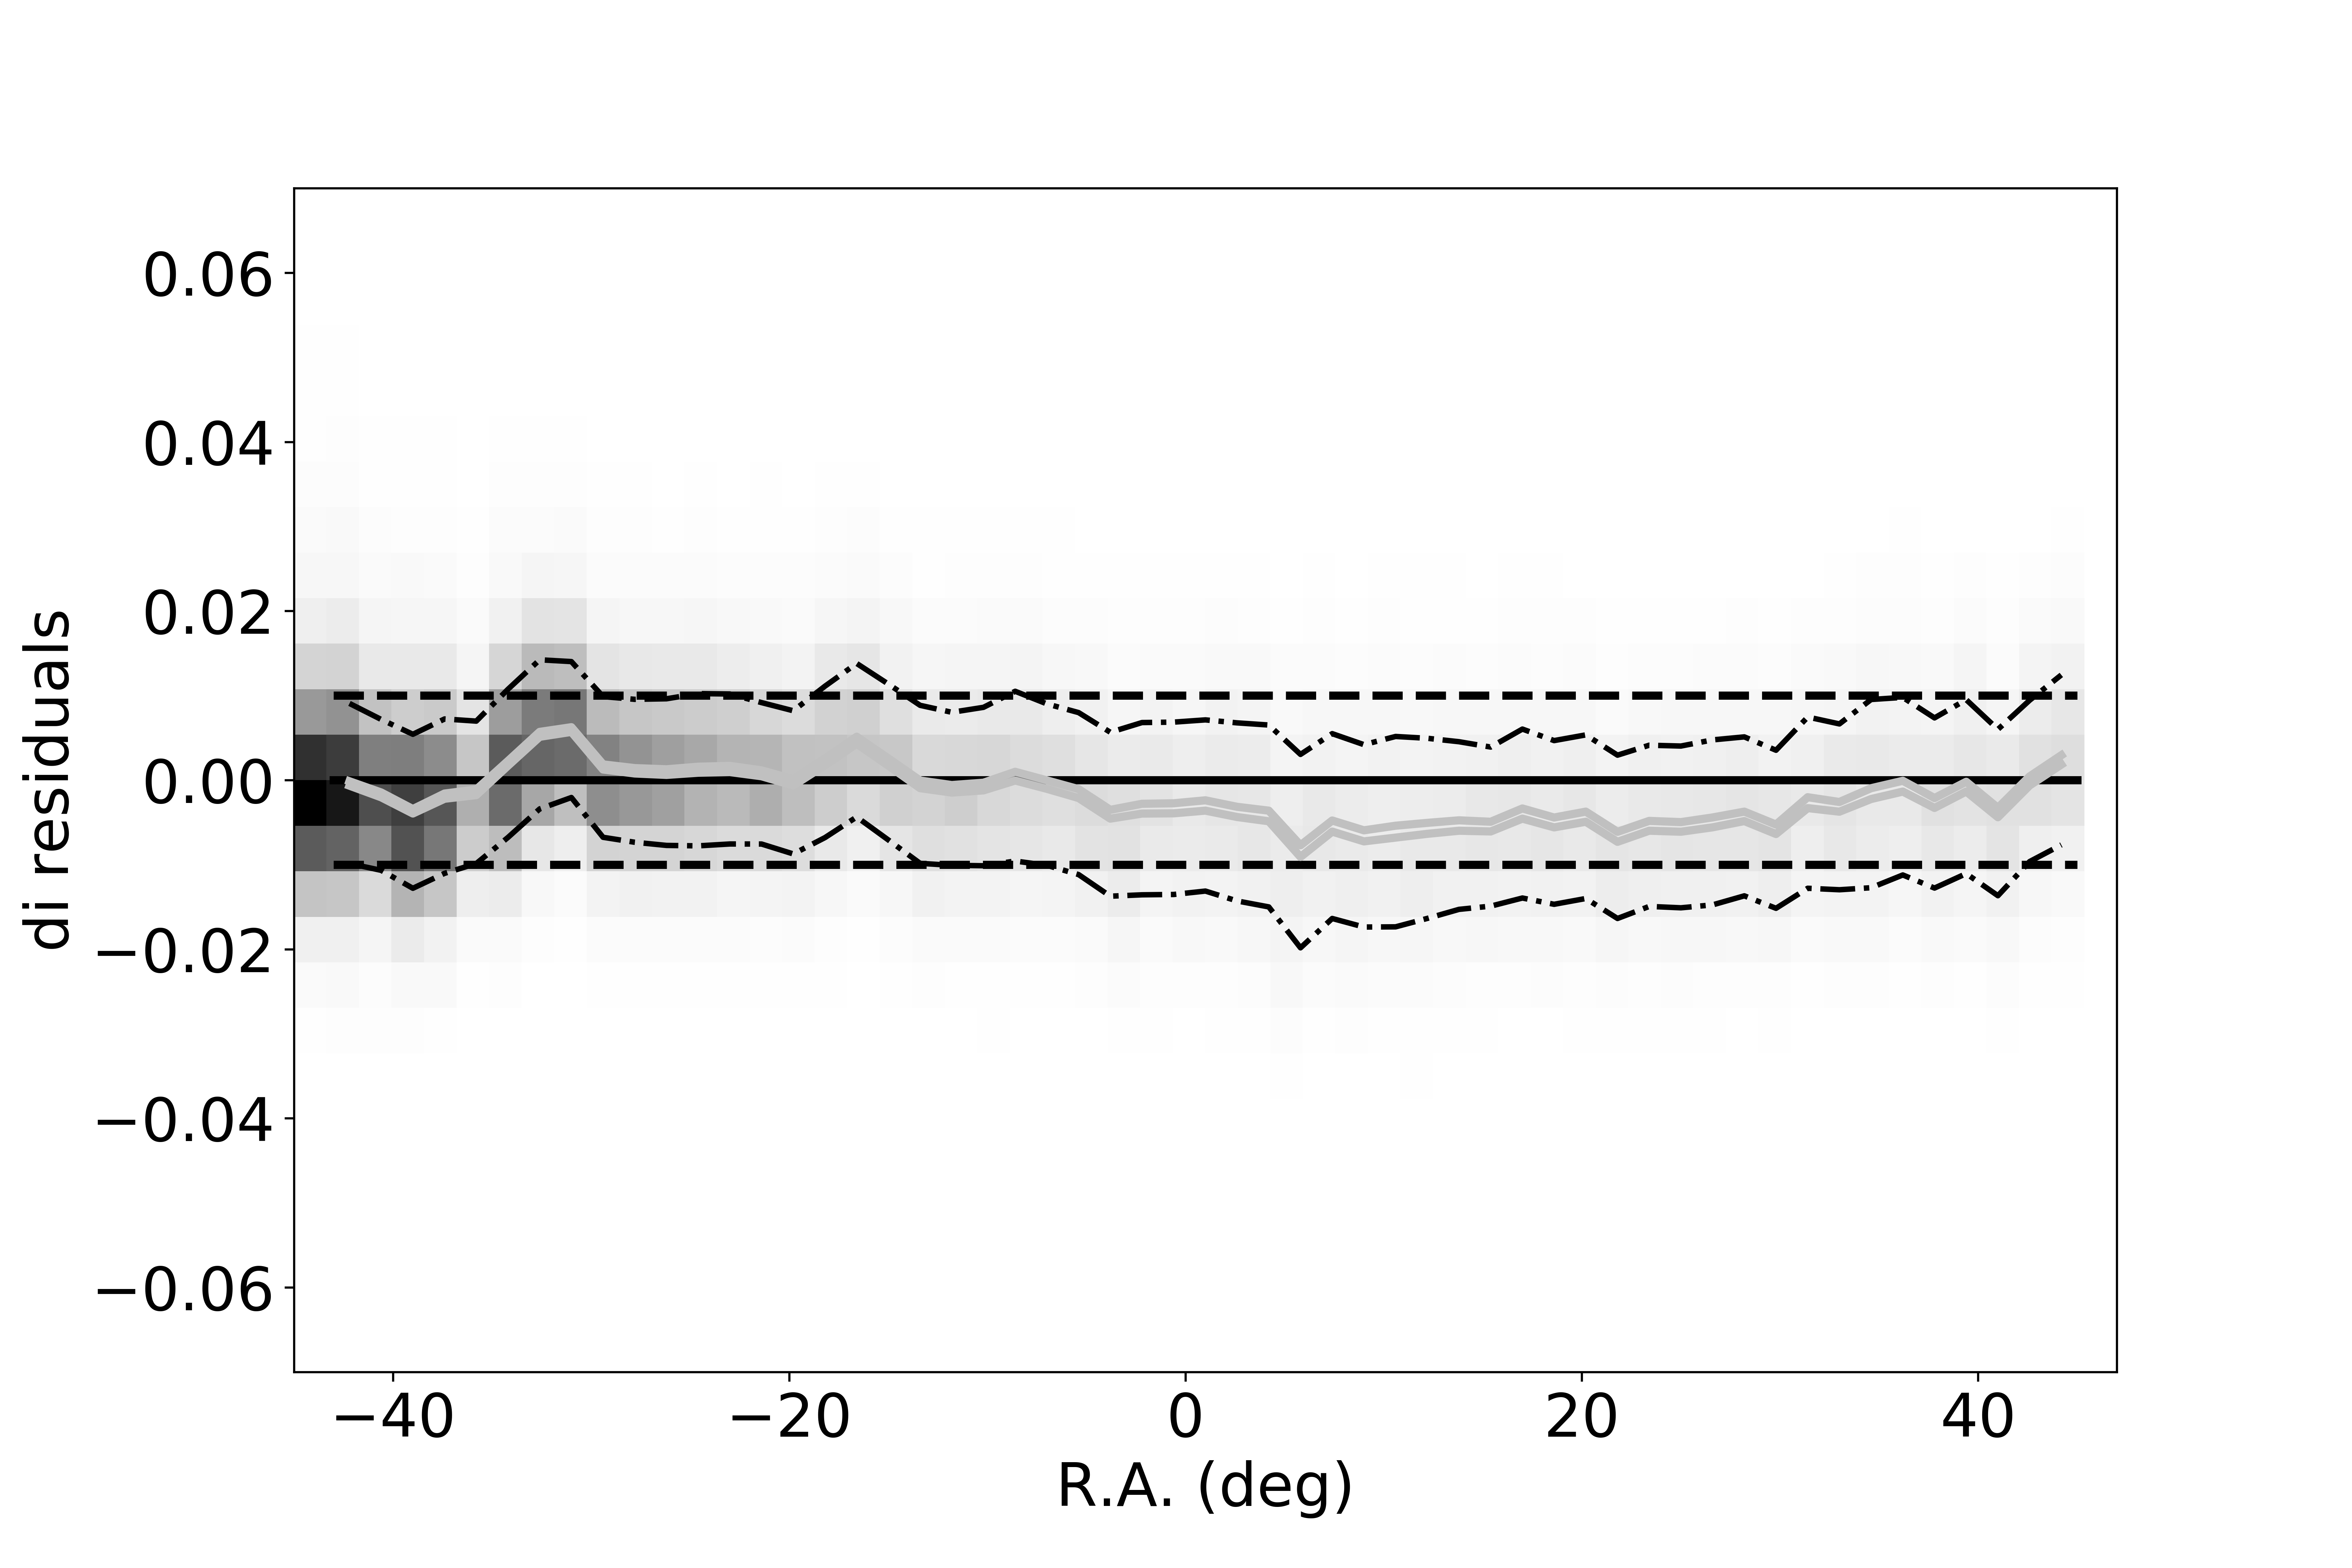
\includegraphics[width=0.45\textwidth]{figures/colorResidPSbright_di_RA_Hess.png}
    \centering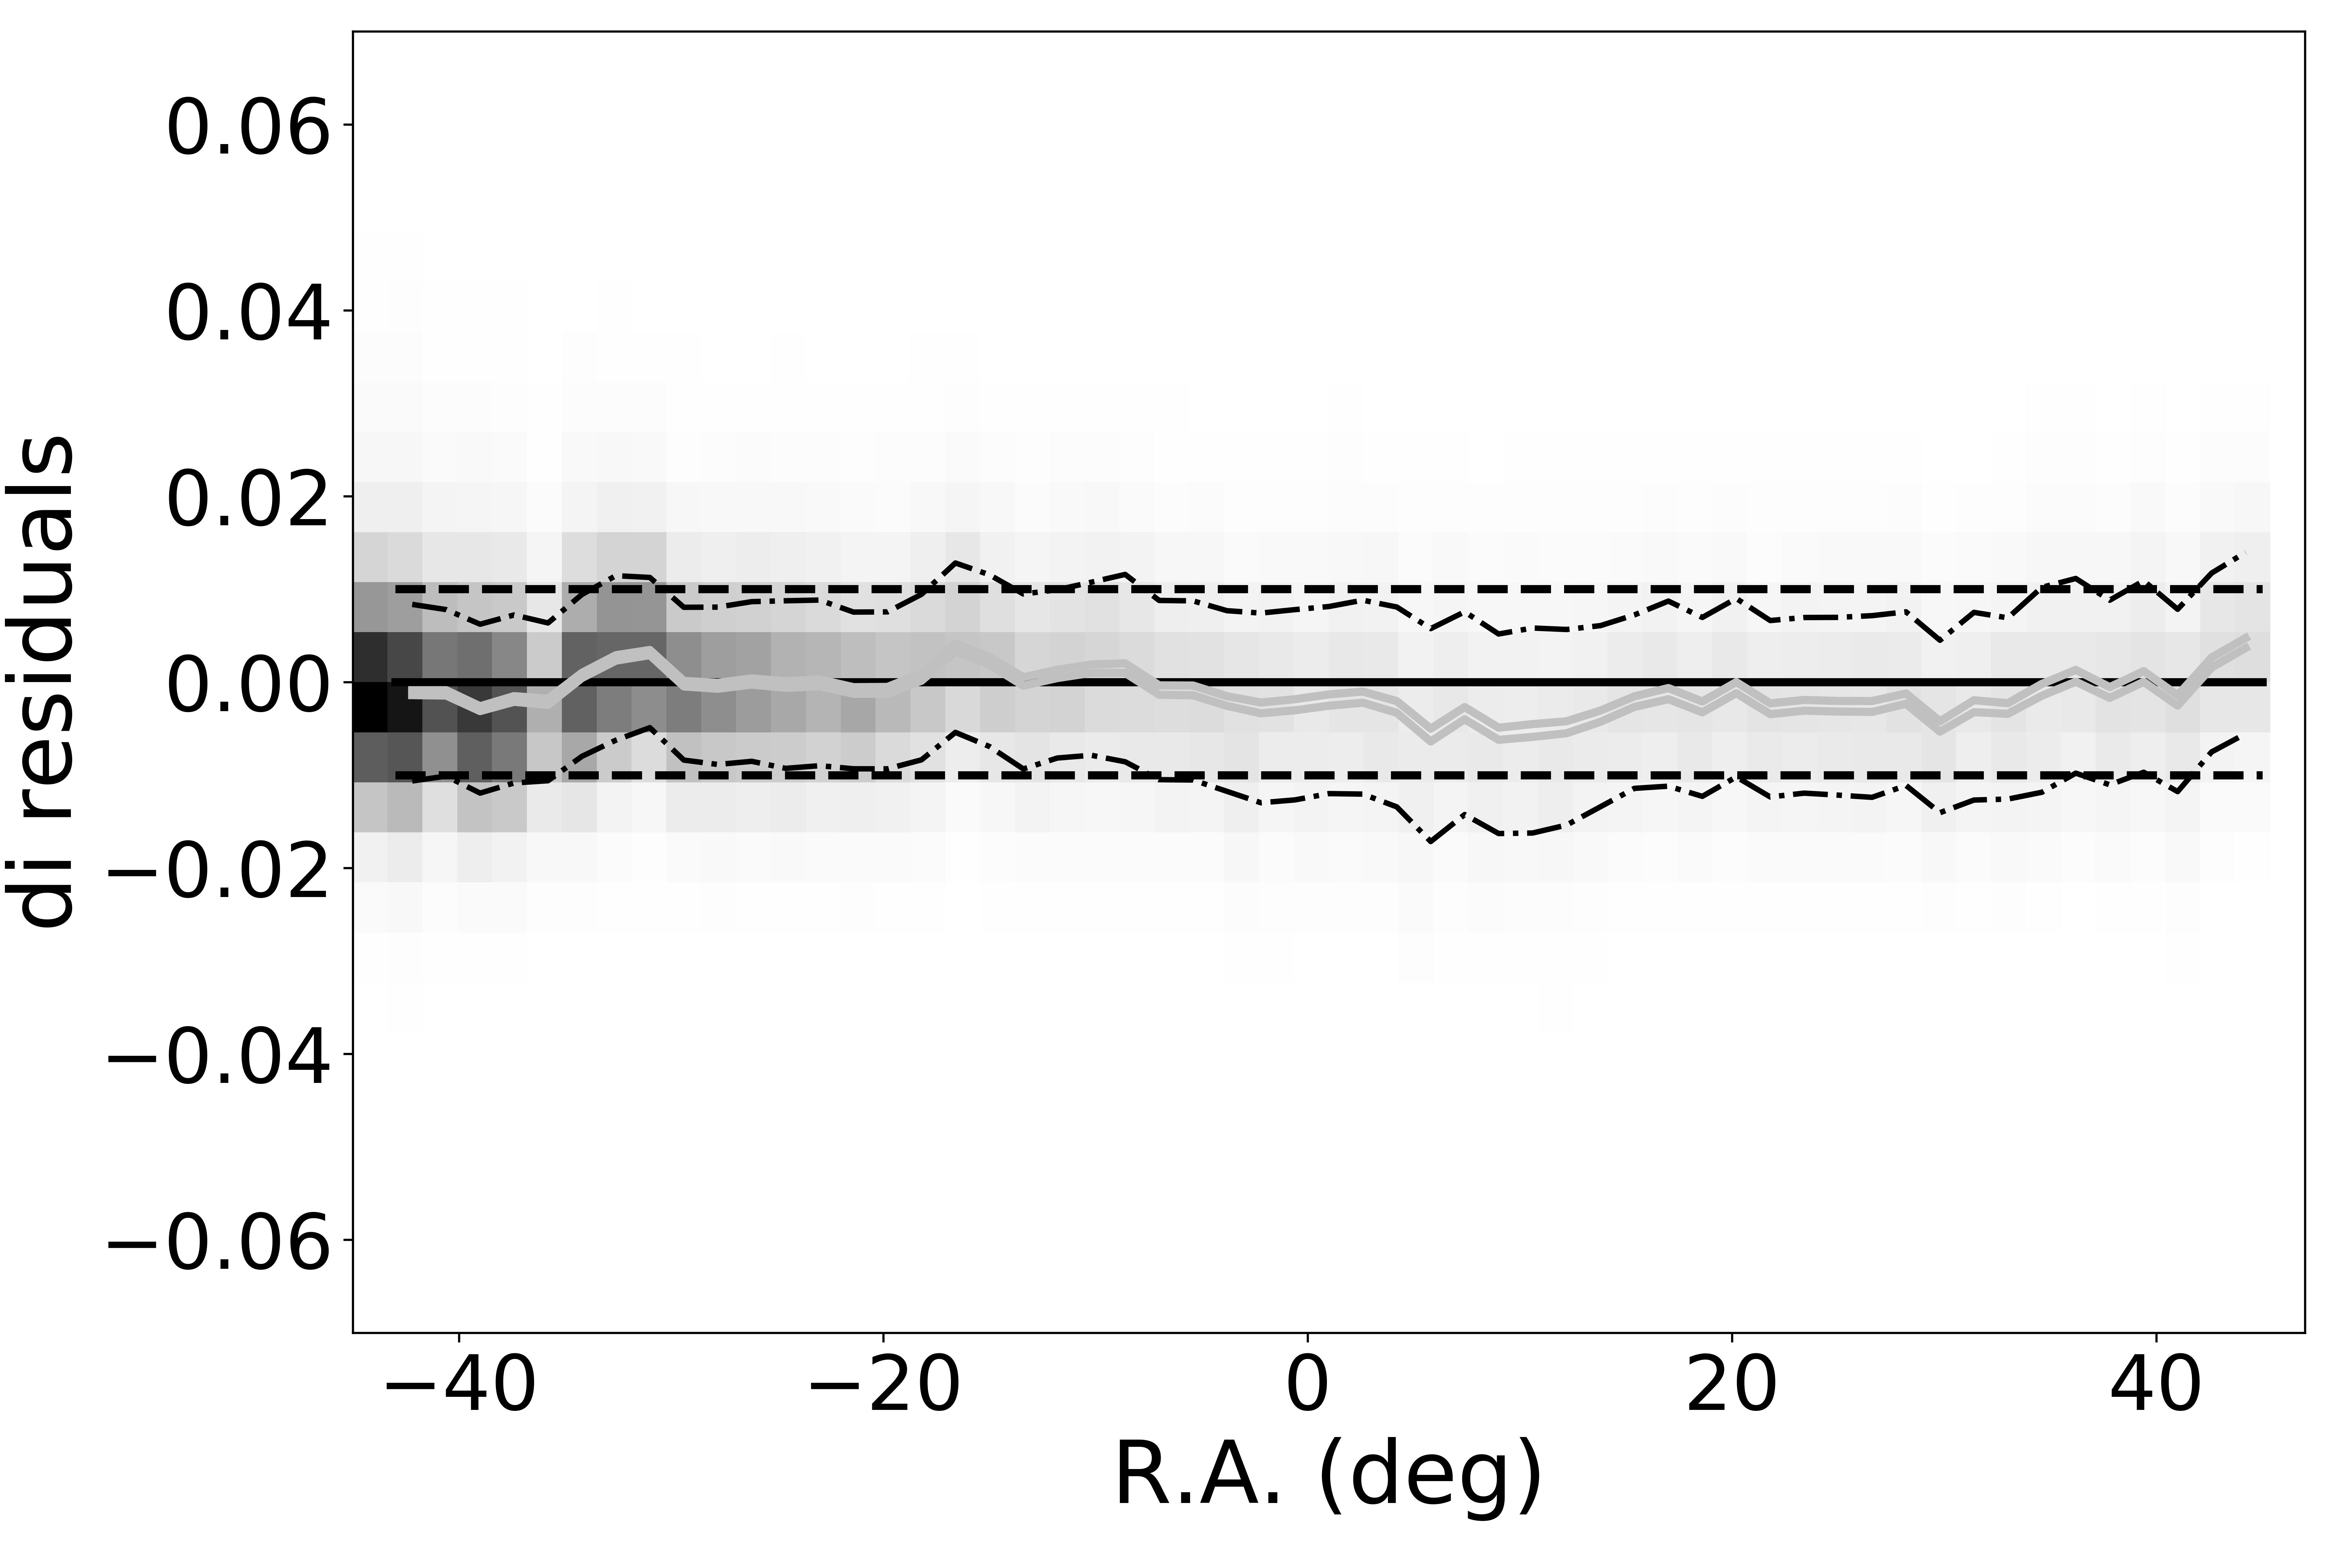
\includegraphics[width=0.45\textwidth]{figures/colorResidPSDR2v42bright_di_RA_Hess.png}
    \centering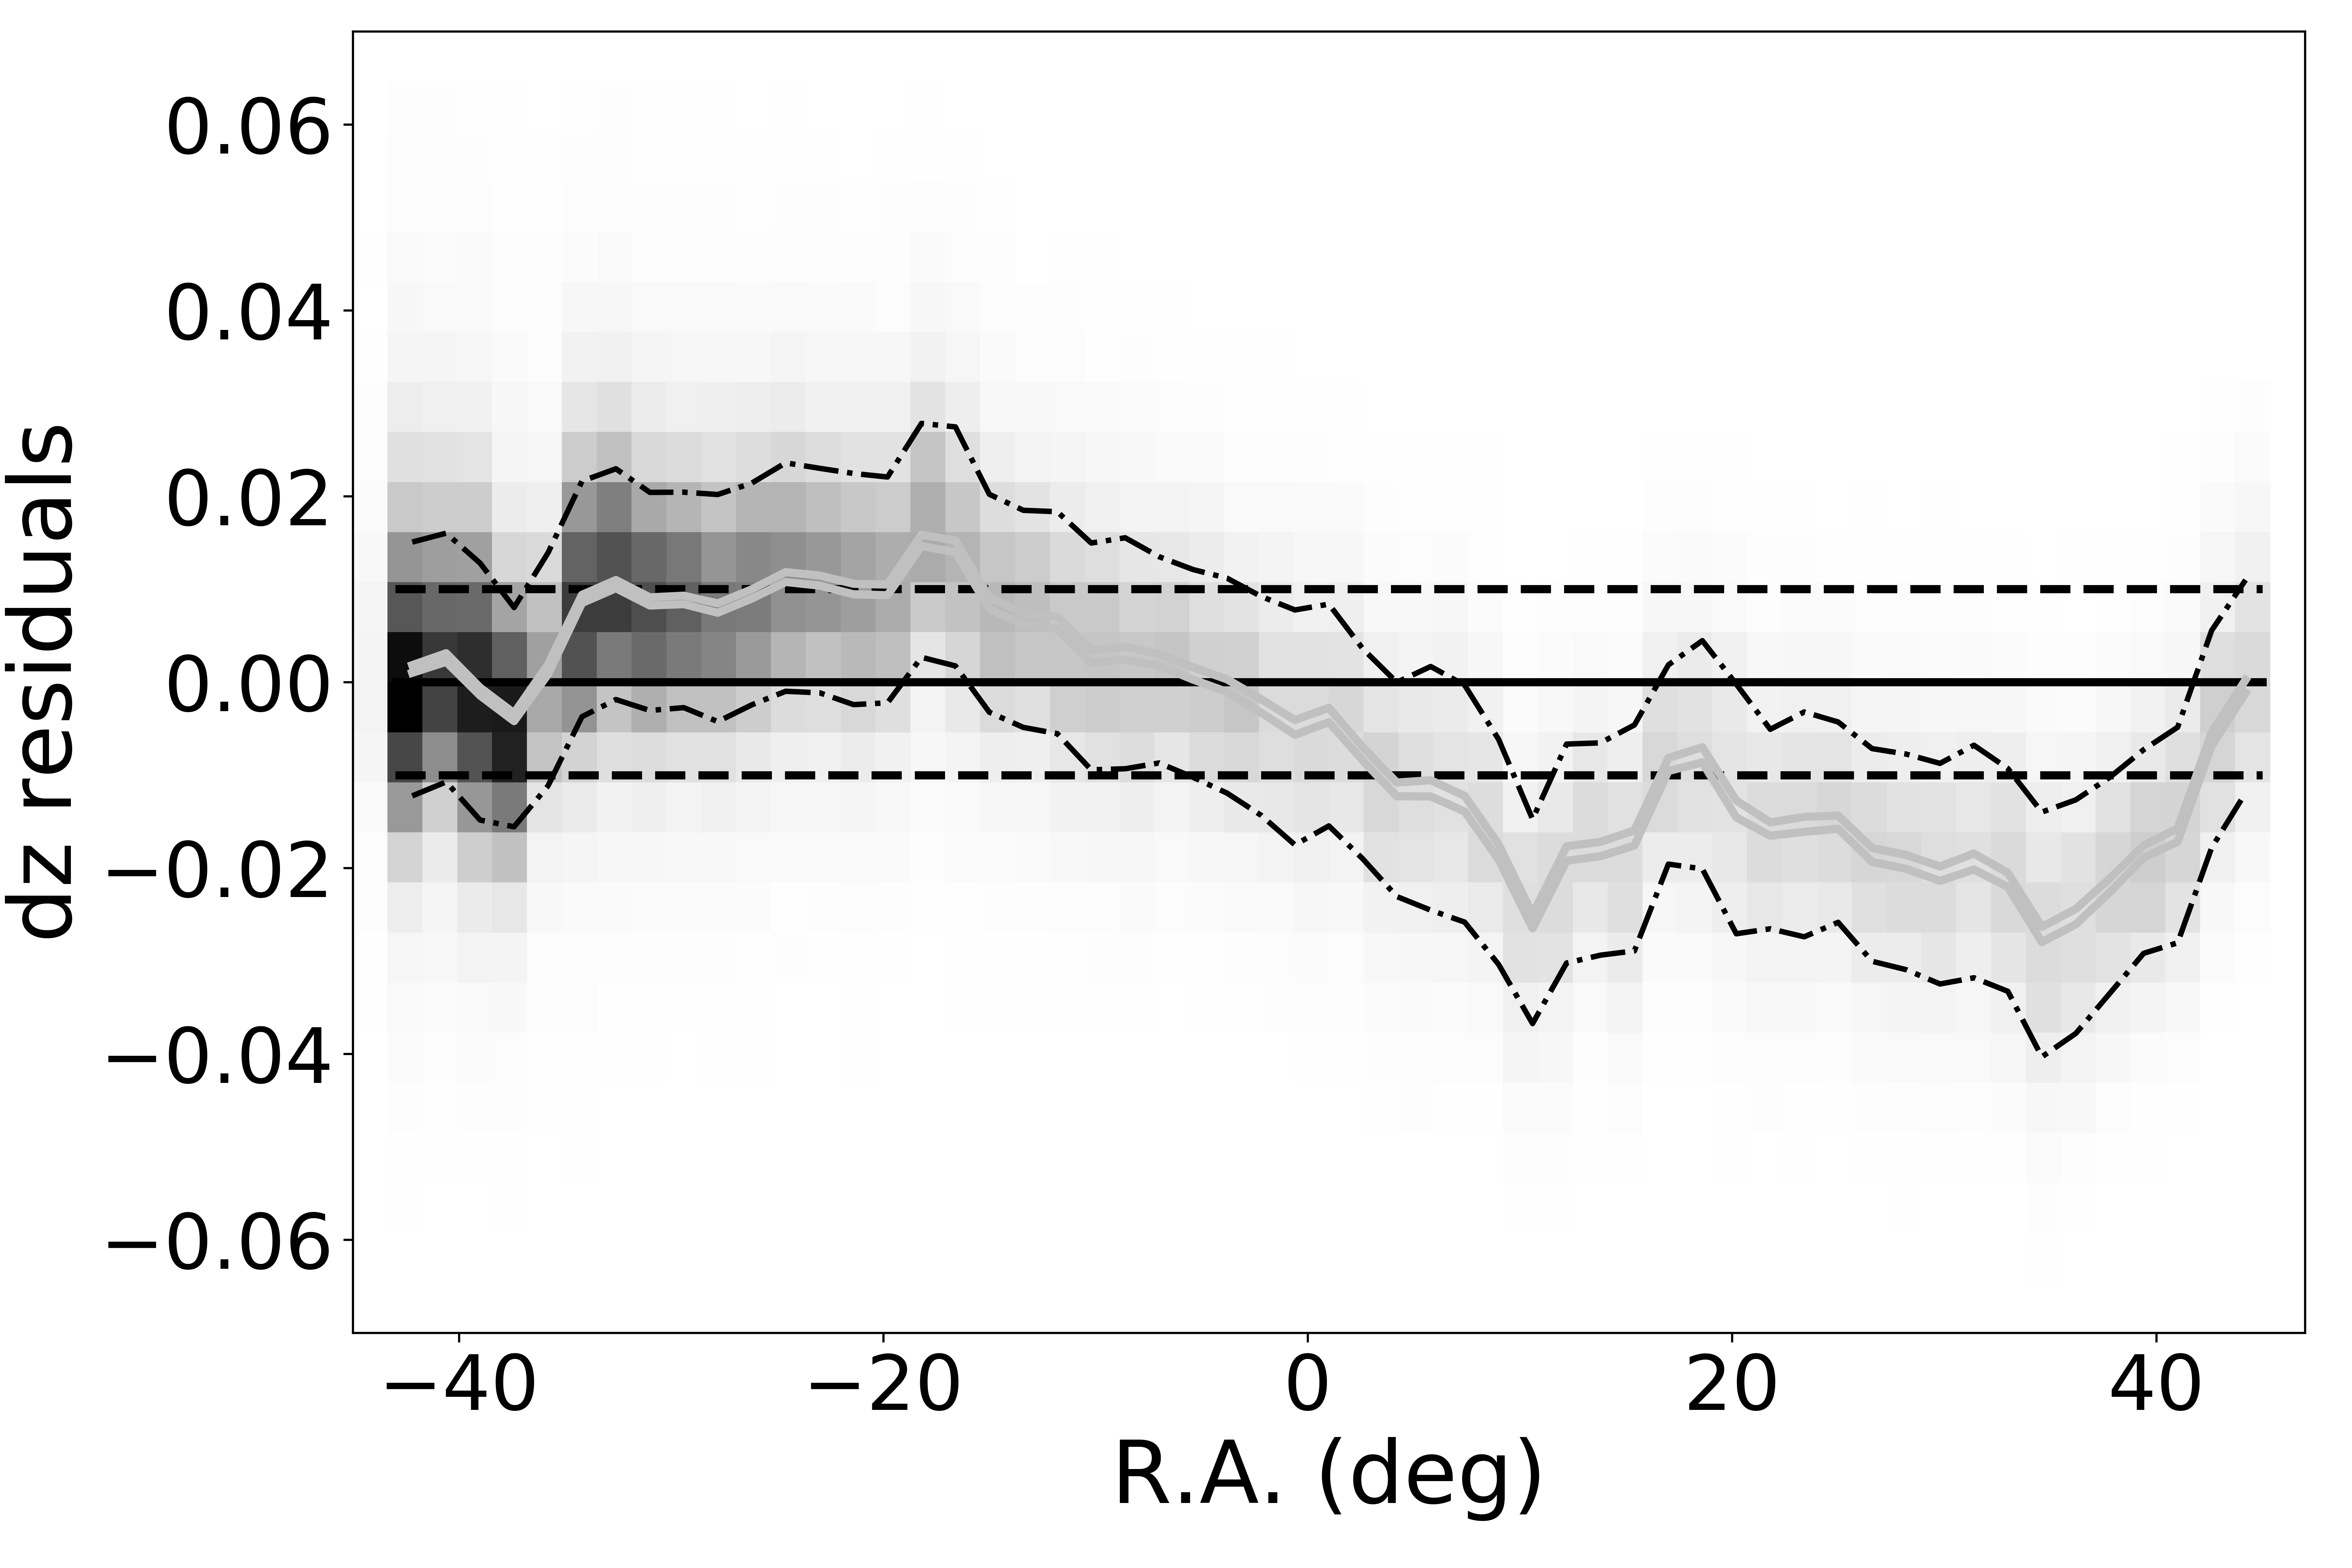
\includegraphics[width=0.45\textwidth]{figures/colorResidDES42bright_dz_RA_Hess.png}
    % \centering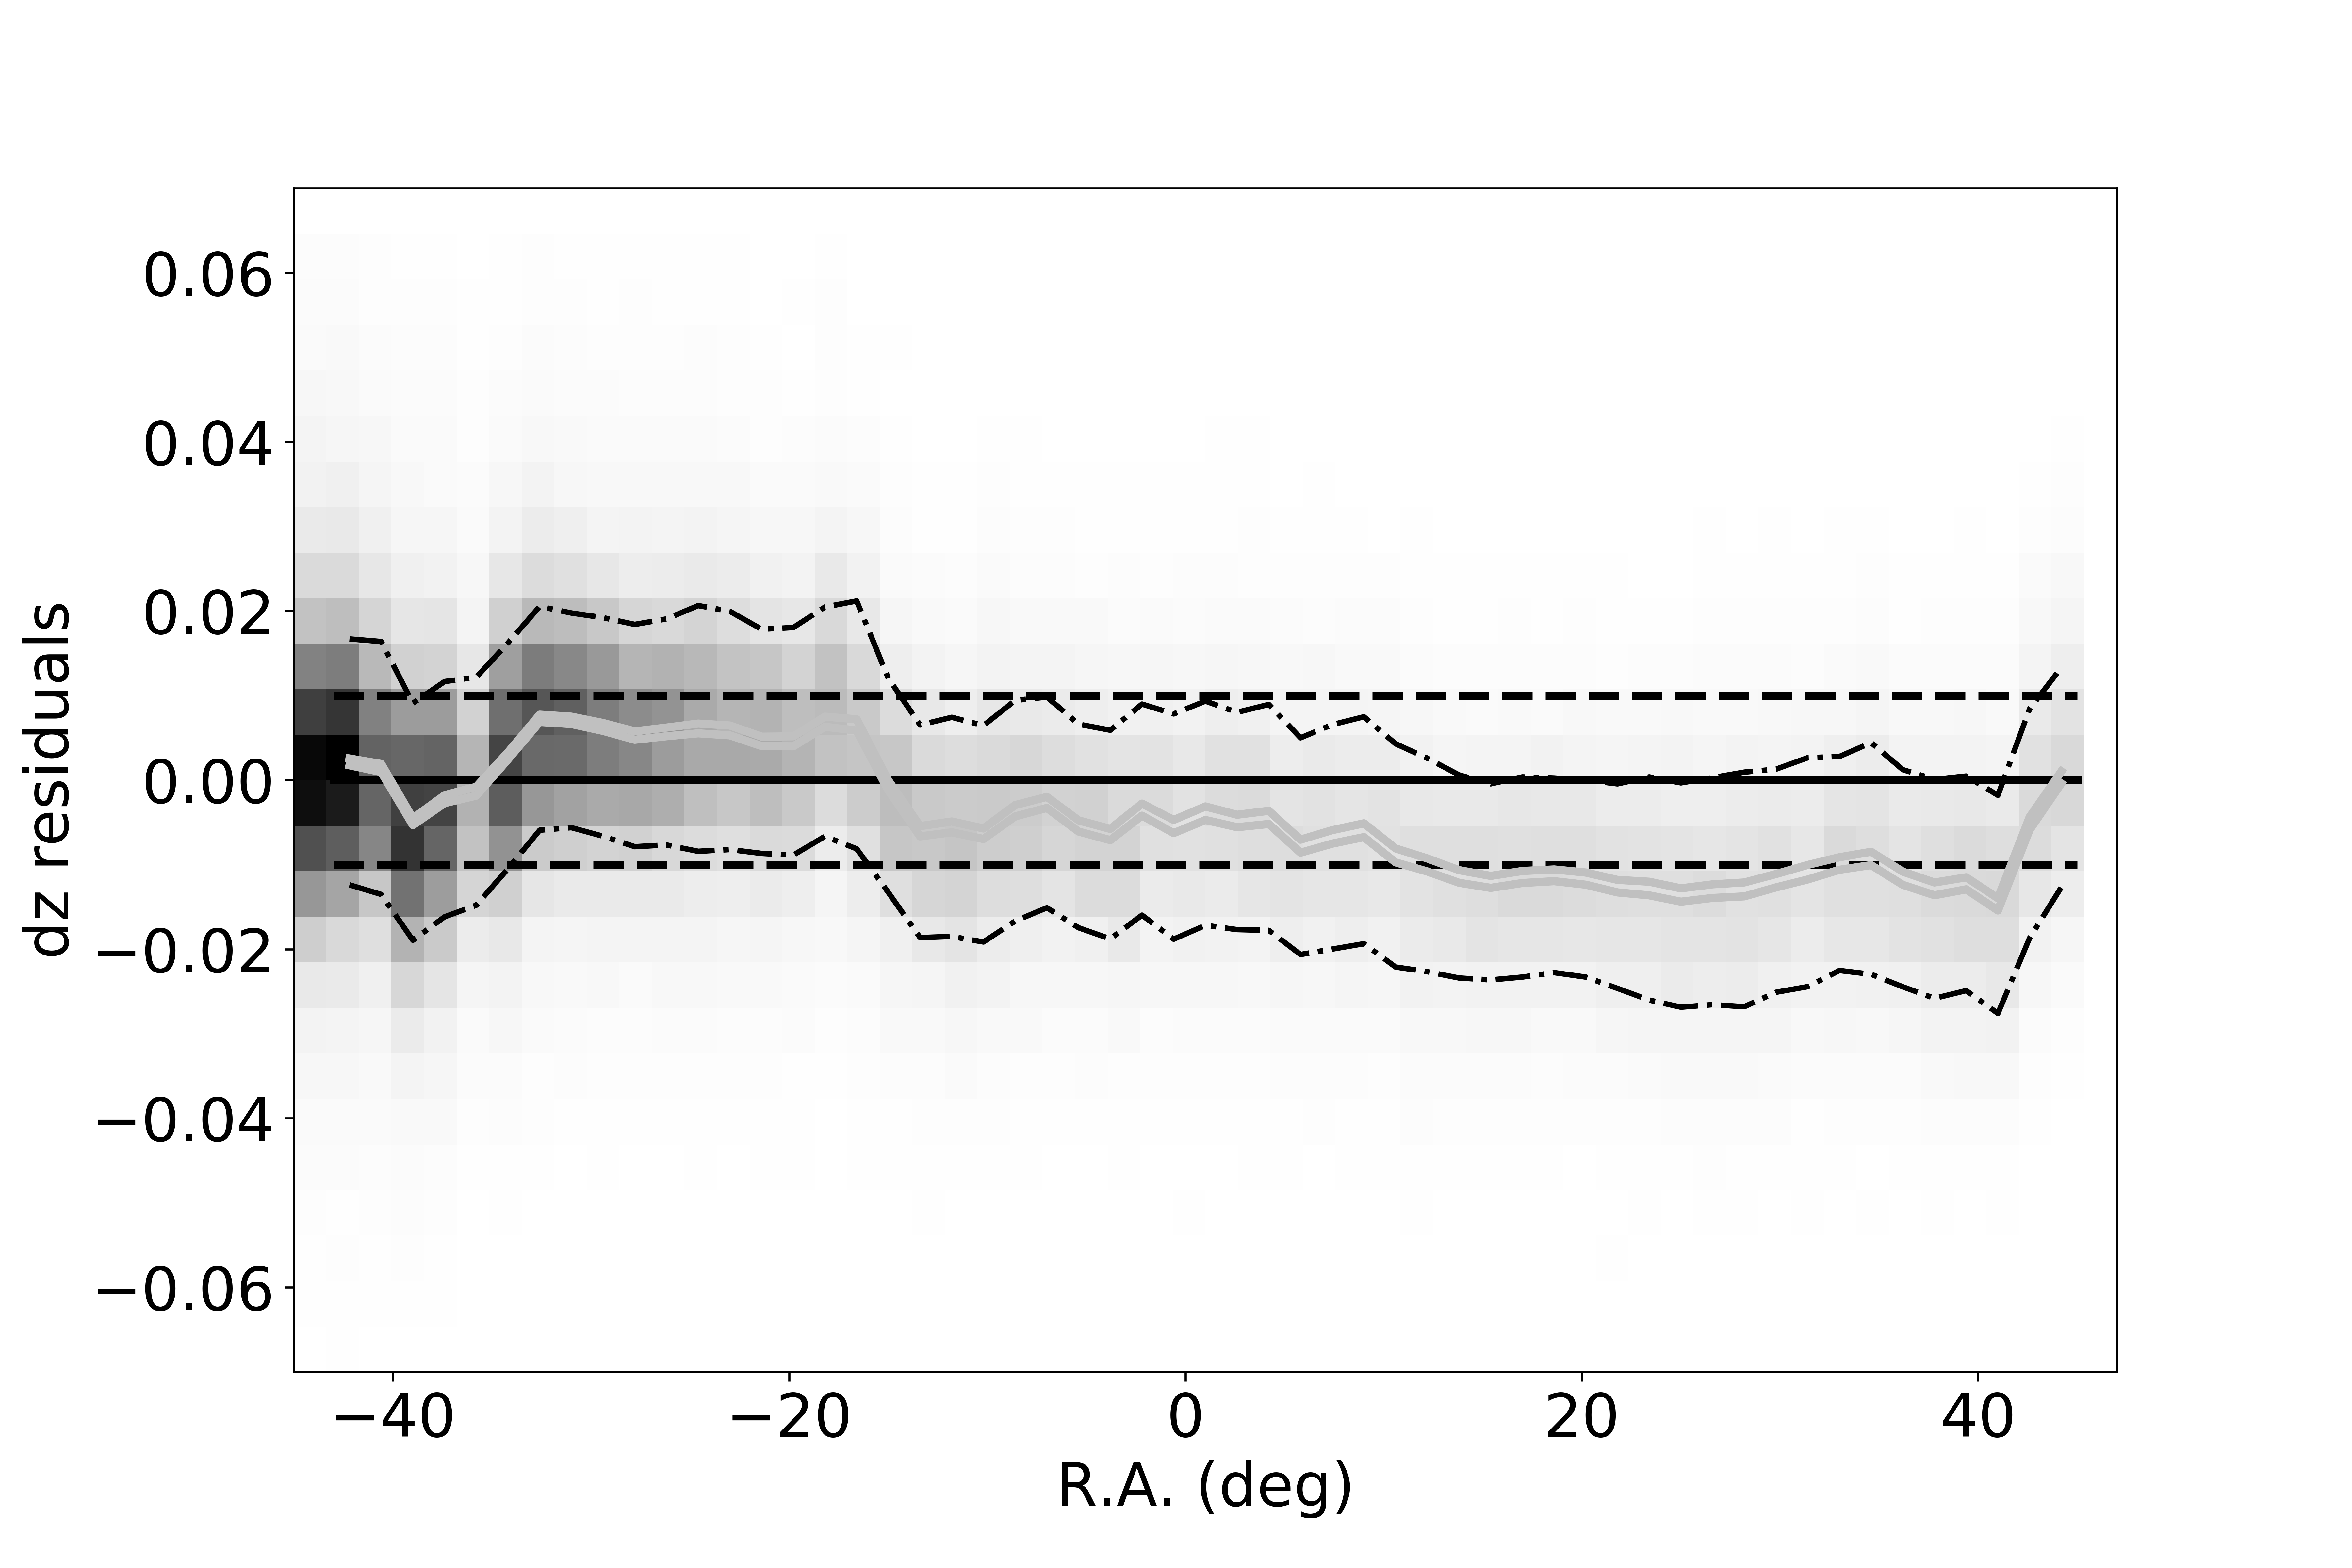
\includegraphics[width=0.45\textwidth]{figures/colorResidPSbright_dz_RA_Hess.png}
    \centering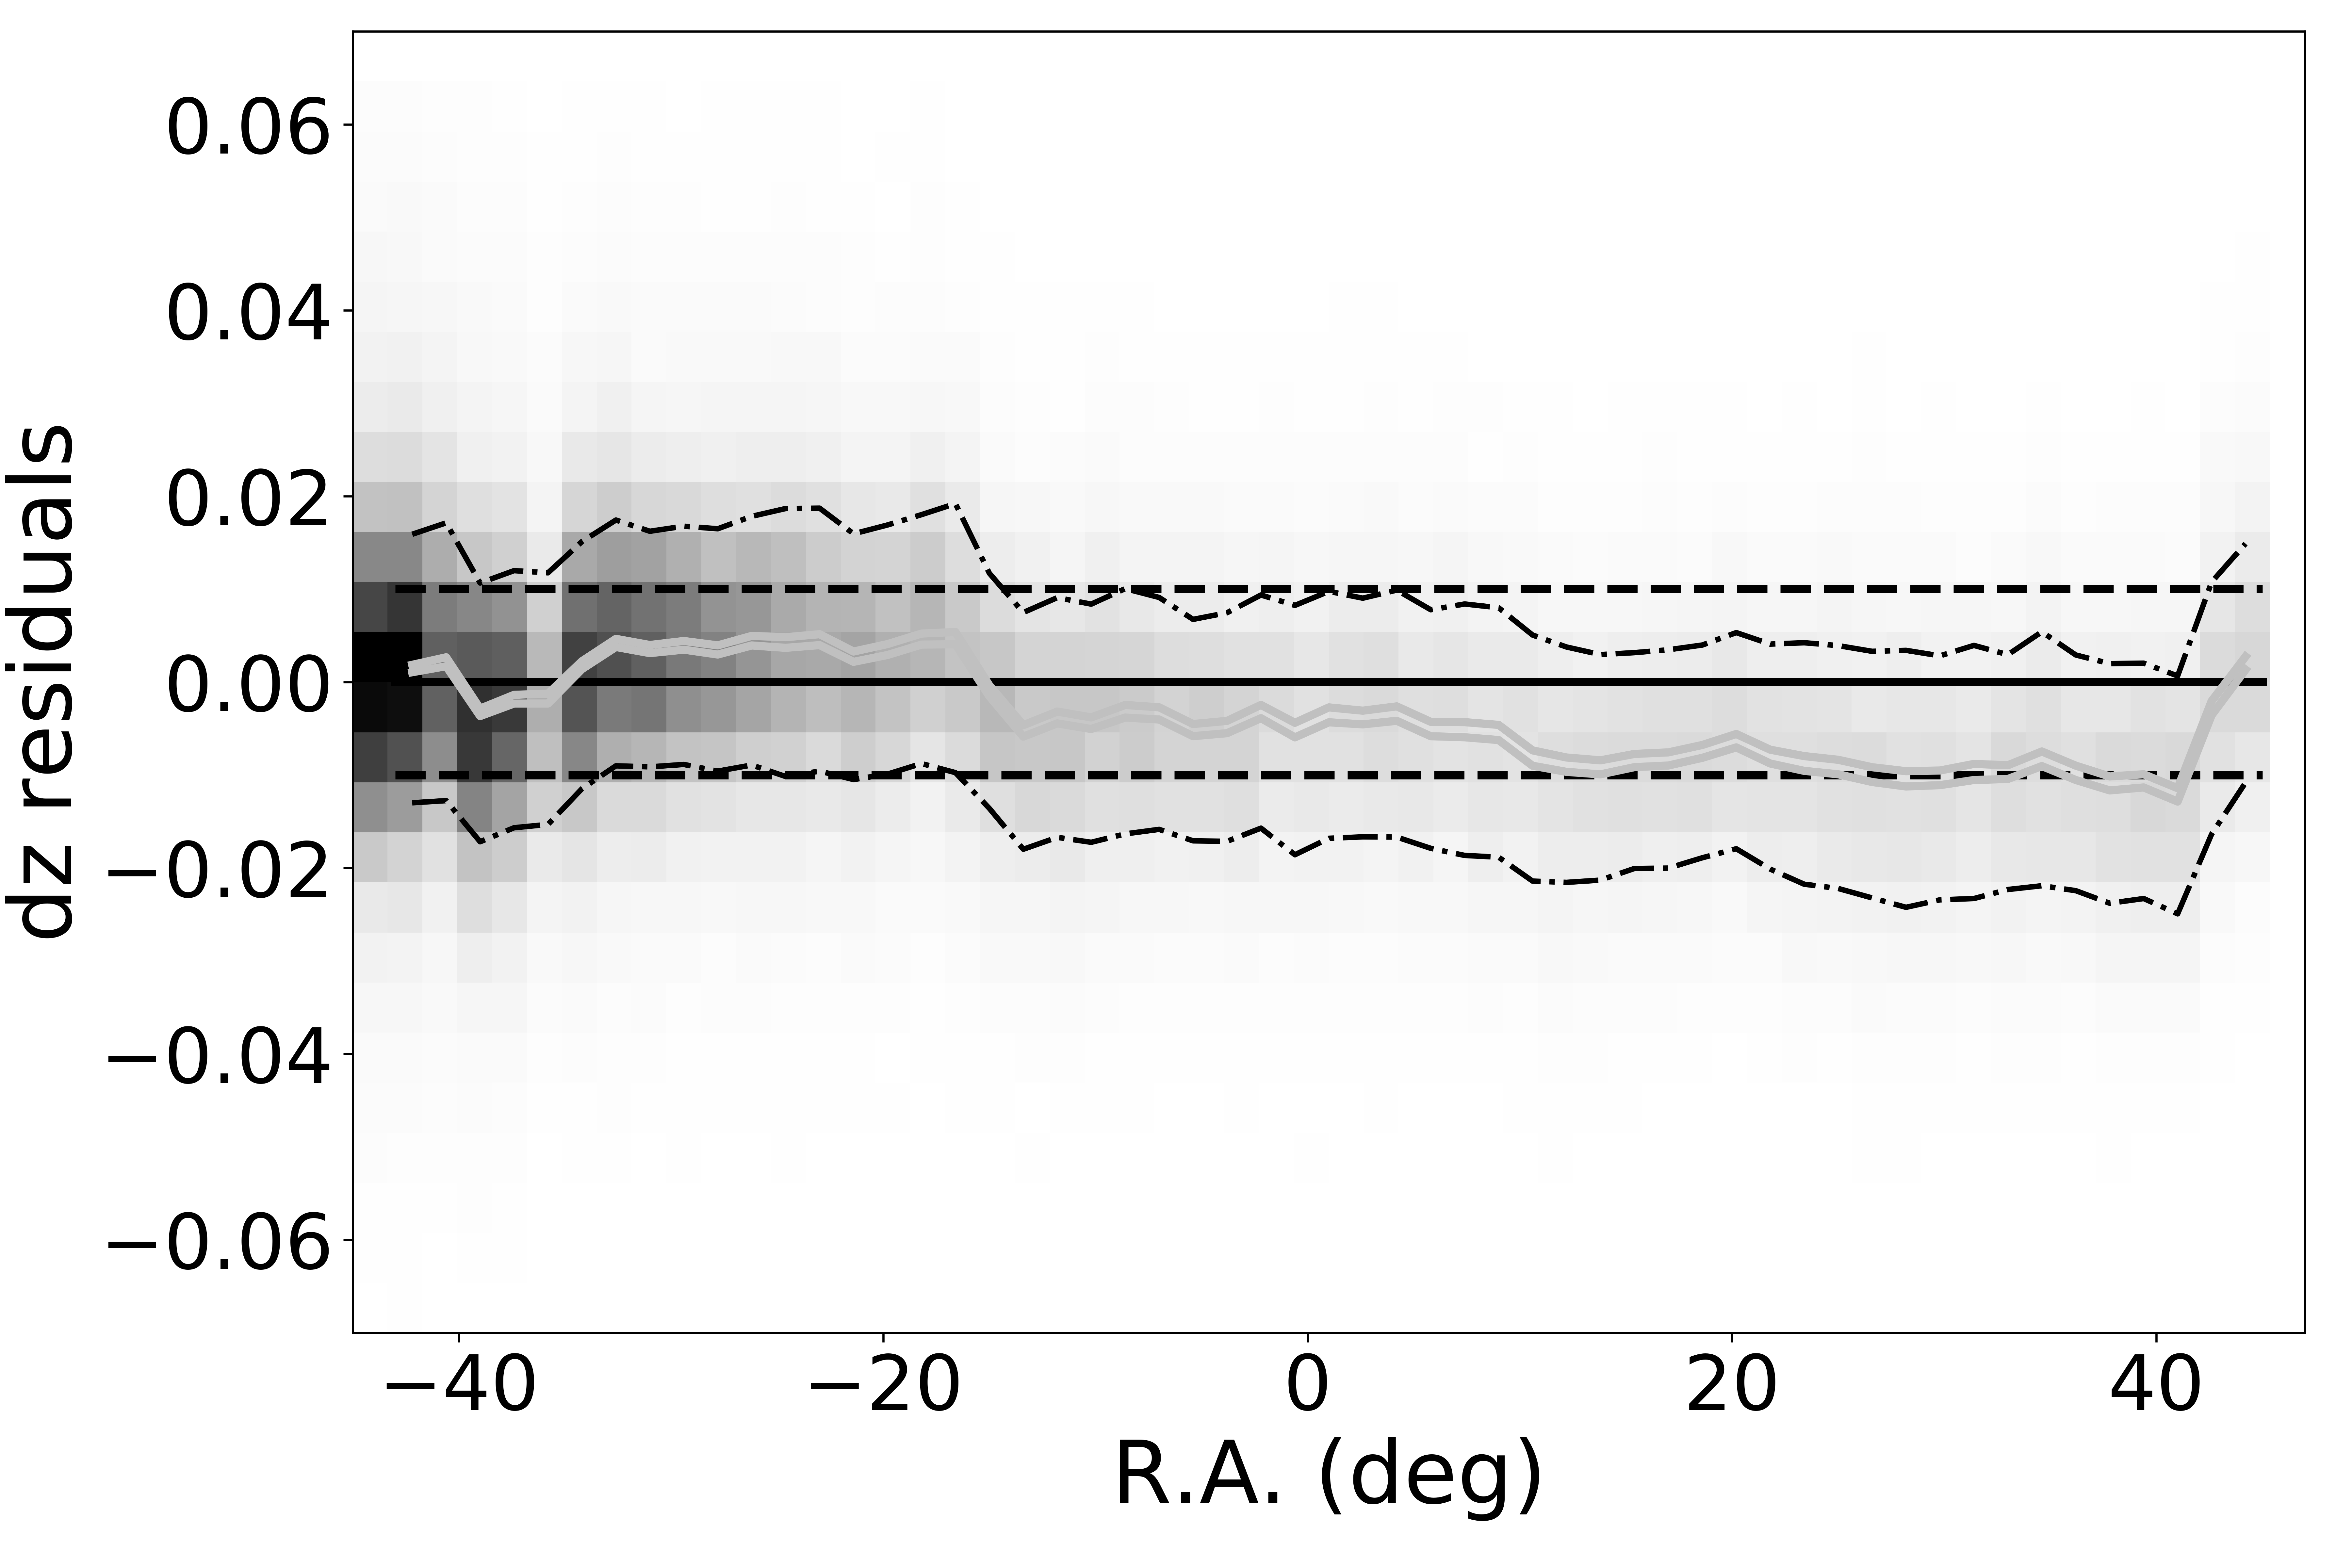
\includegraphics[width=0.45\textwidth]{figures/colorResidPSDR2v42bright_dz_RA_Hess.png}
\caption{A comparison of the magnitude differences between the SDSS v4.2 catalog
and DES (left) and Pan-STARRS (right) catalogs, for the $riz$ bands.}
\label{fig:DESPSRA}
\end{figure*}

\begin{figure*}
    \centering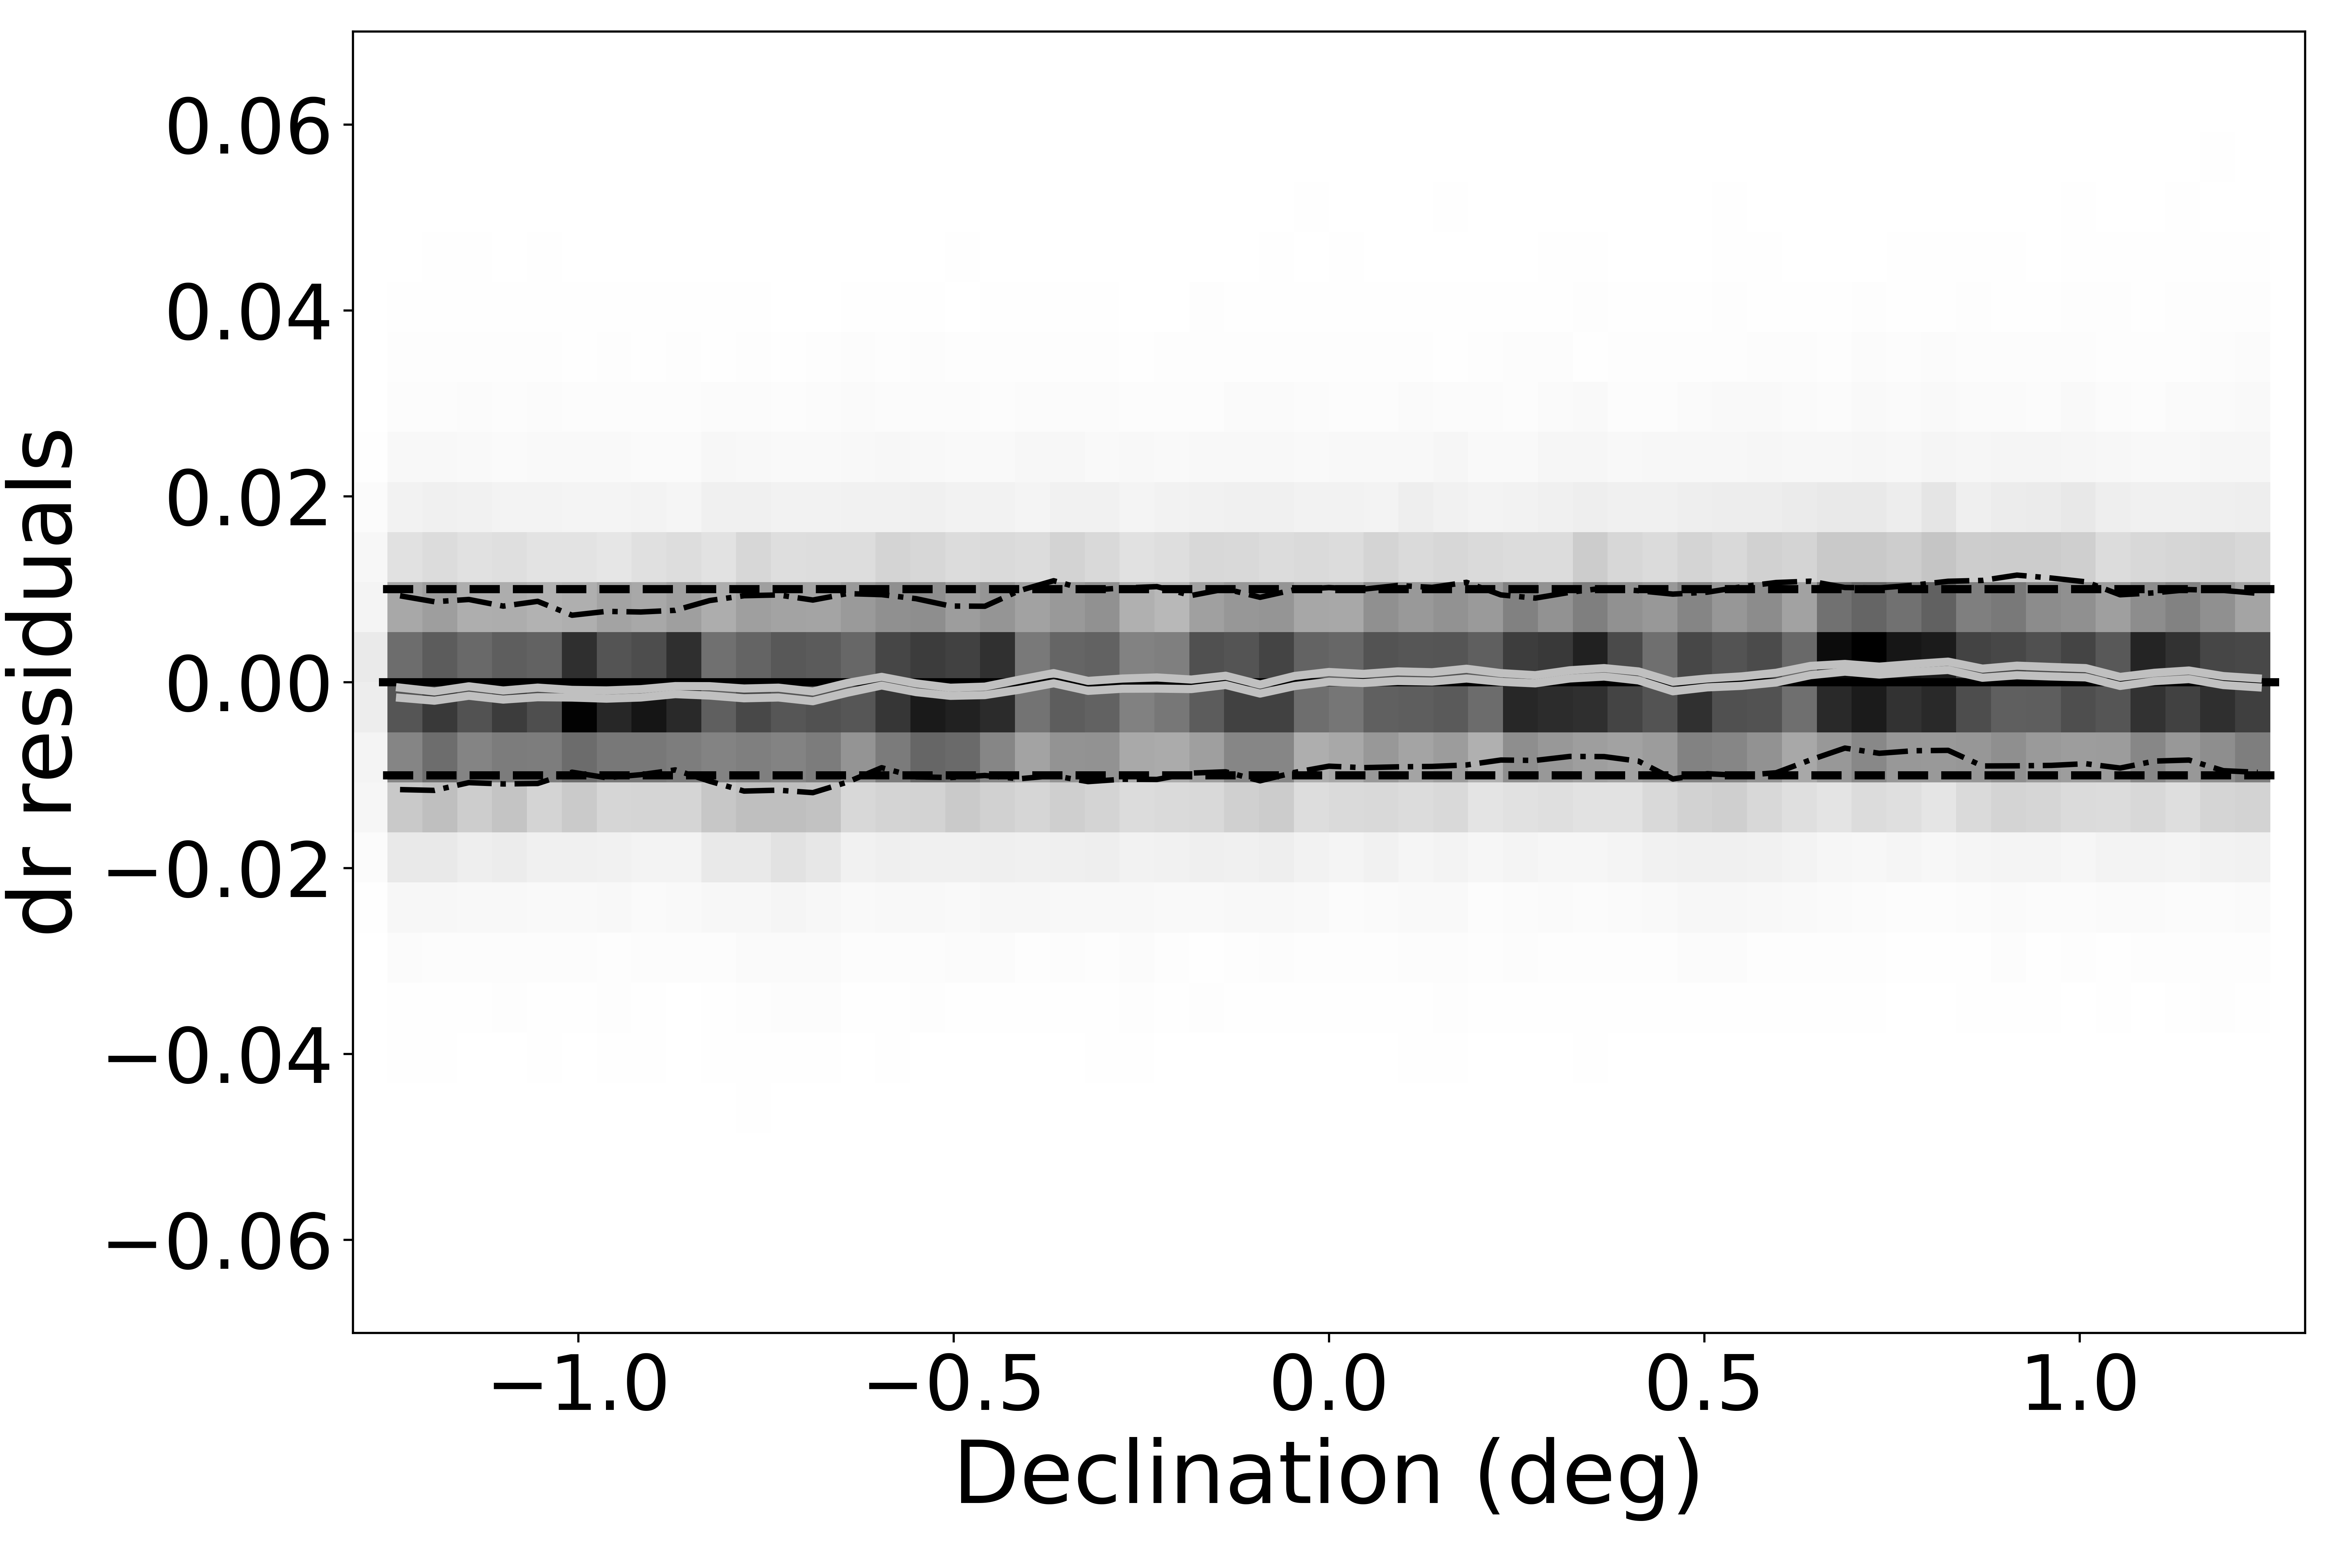
\includegraphics[width=0.45\textwidth]{figures/colorResidDES42bright_dr_Dec_Hess.png}
    % \centering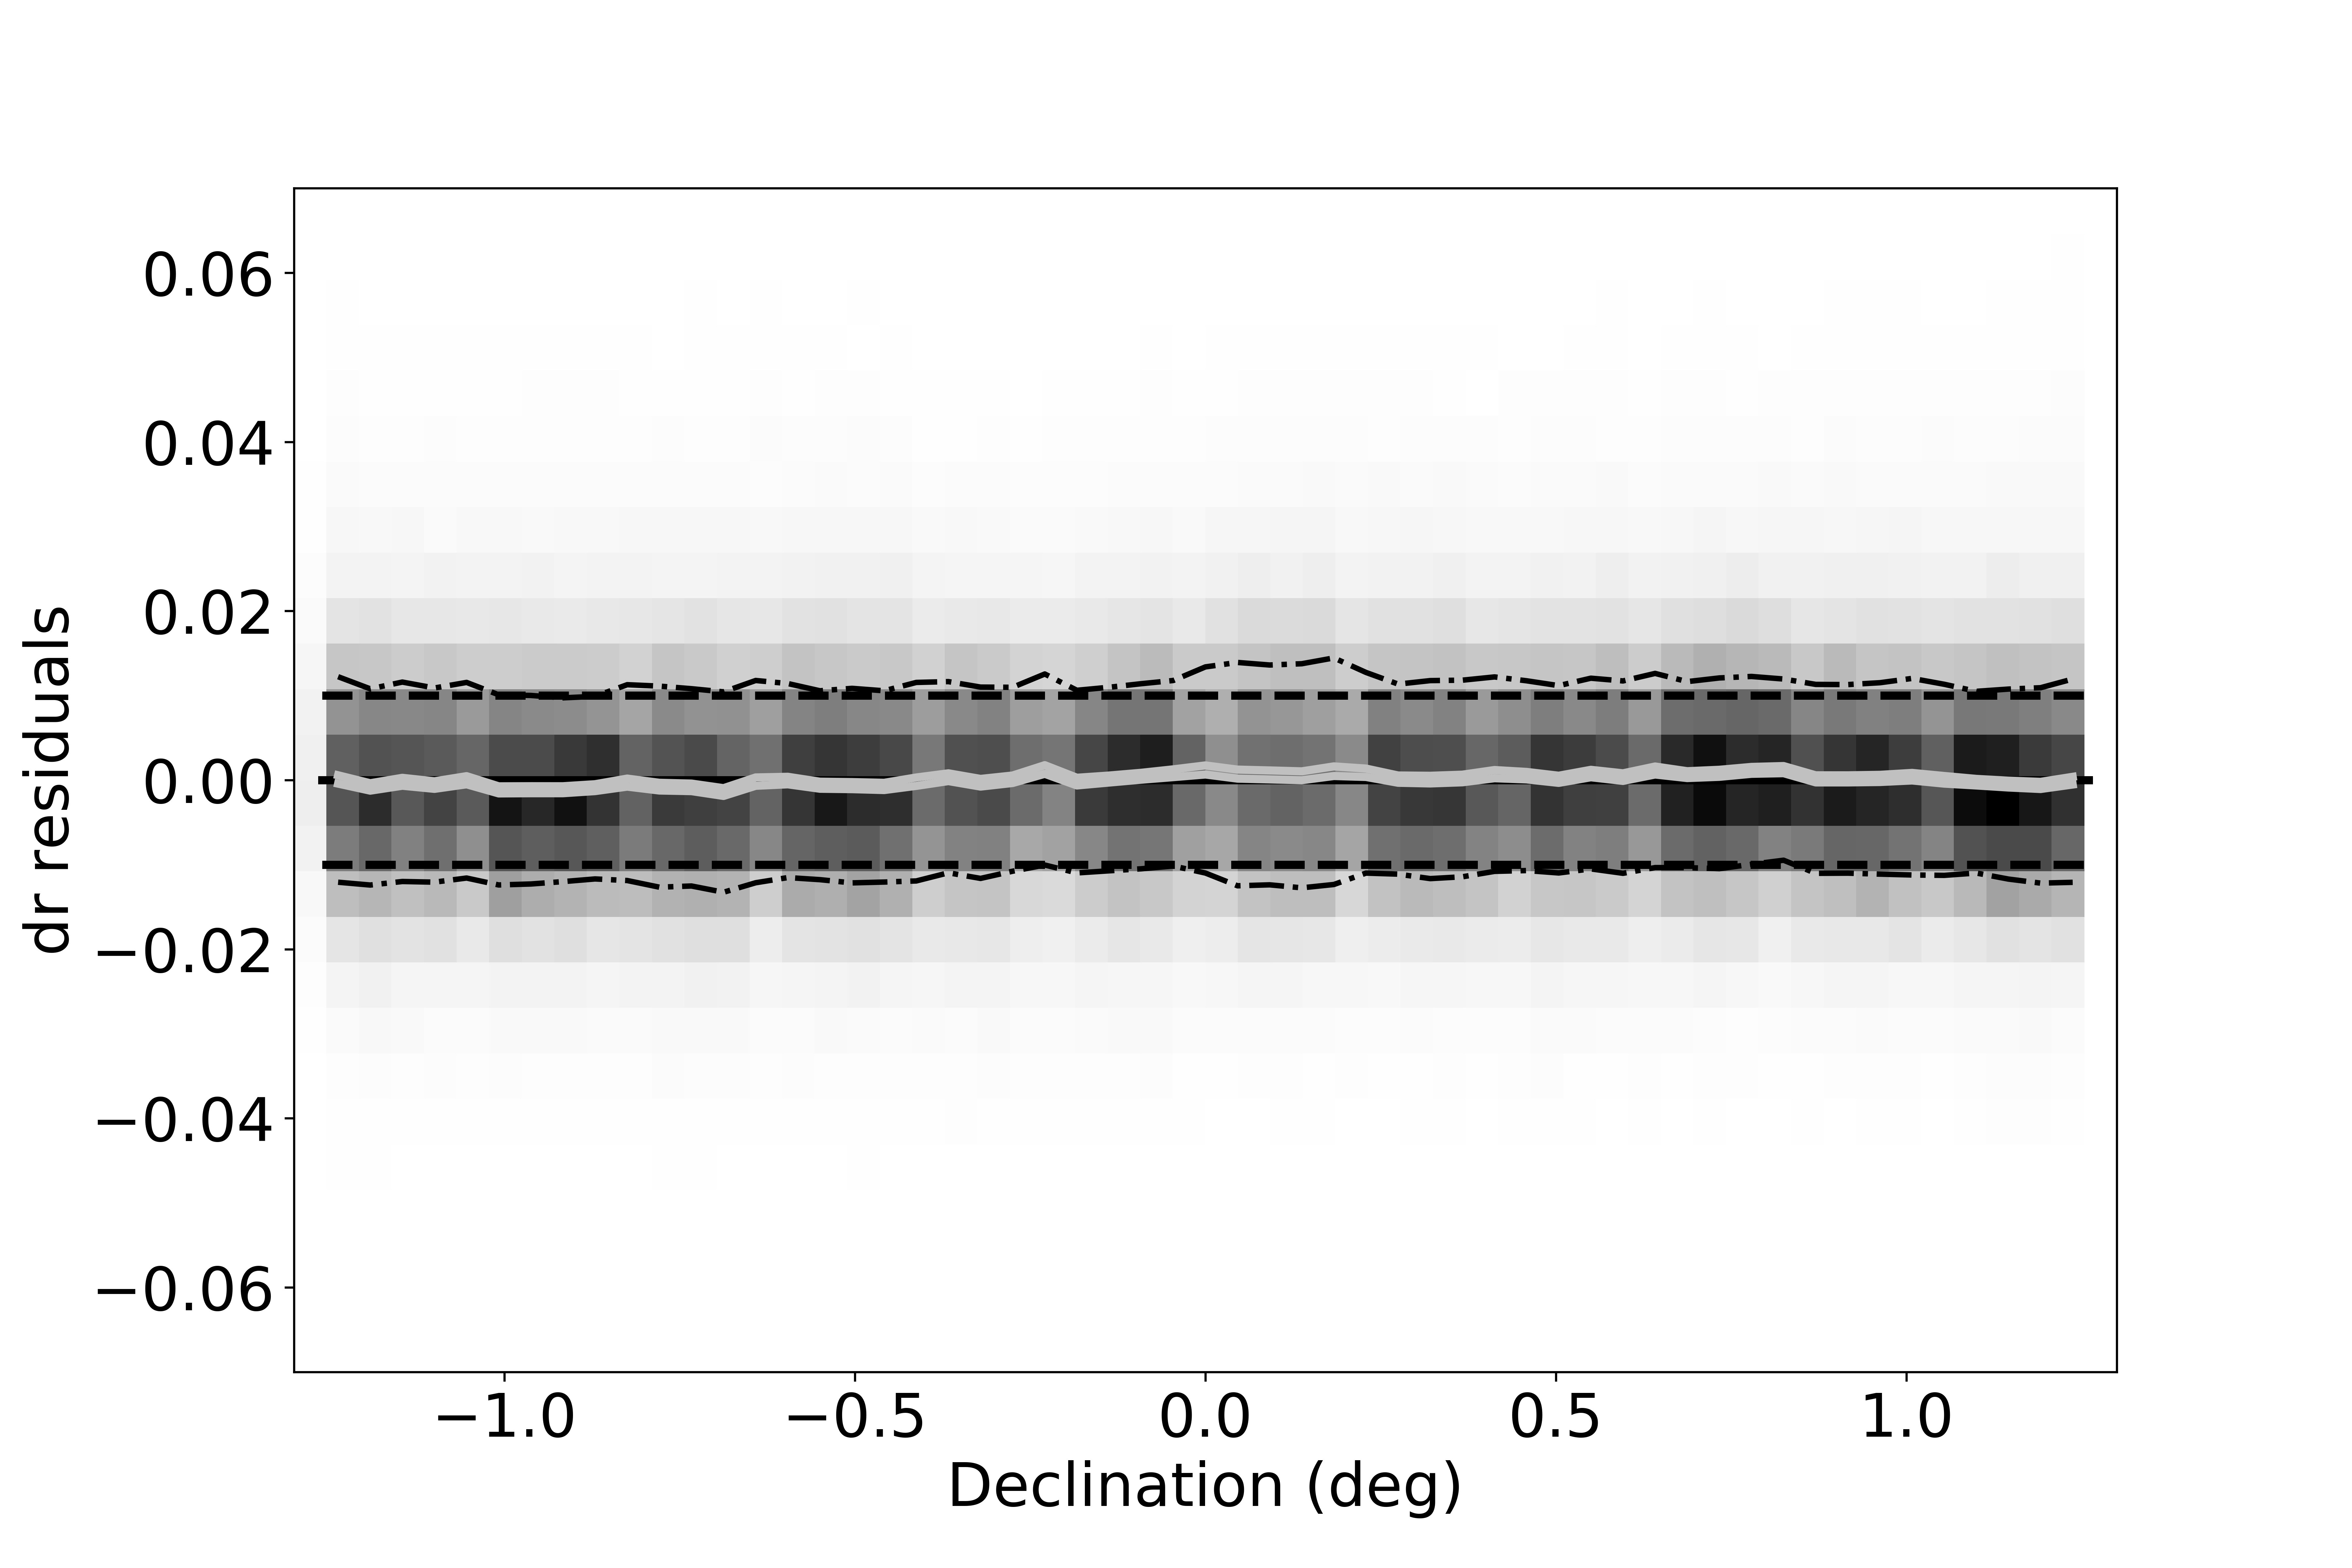
\includegraphics[width=0.45\textwidth]{figures/colorResidPSbright_dr_Dec_Hess.png}
    \centering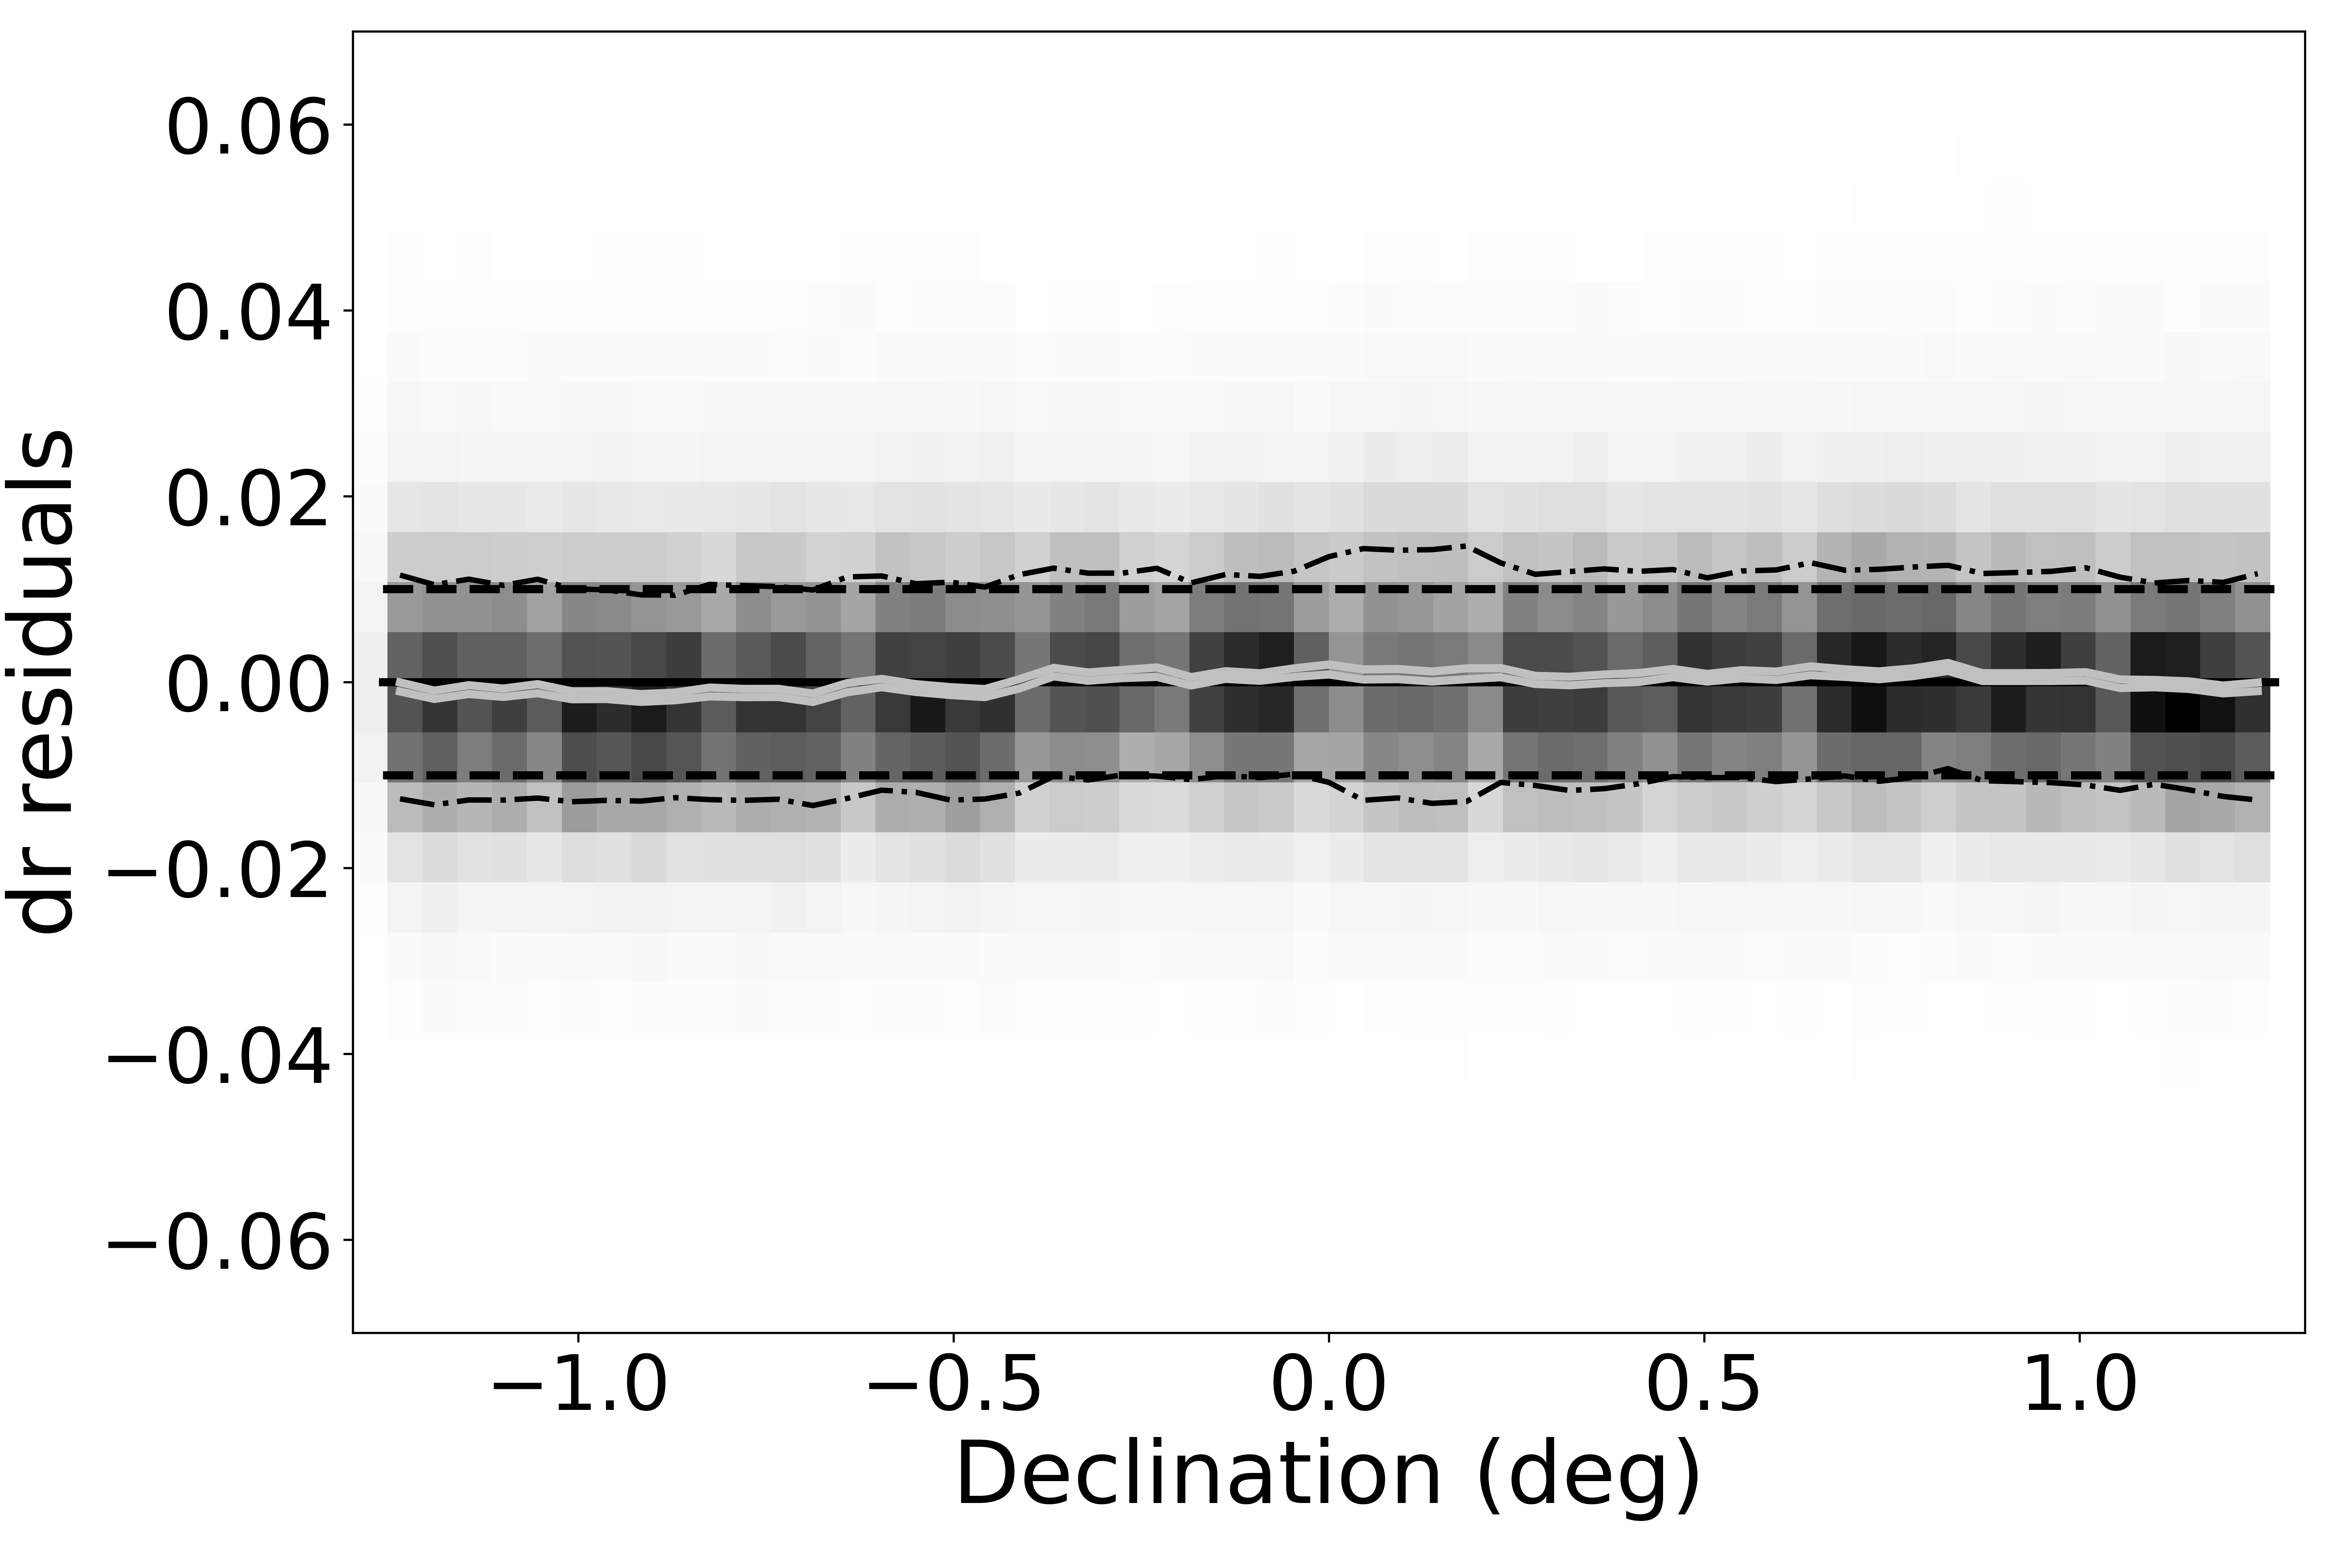
\includegraphics[width=0.45\textwidth]{figures/colorResidPSDR2v42bright_dr_Dec_Hess.png}
    \centering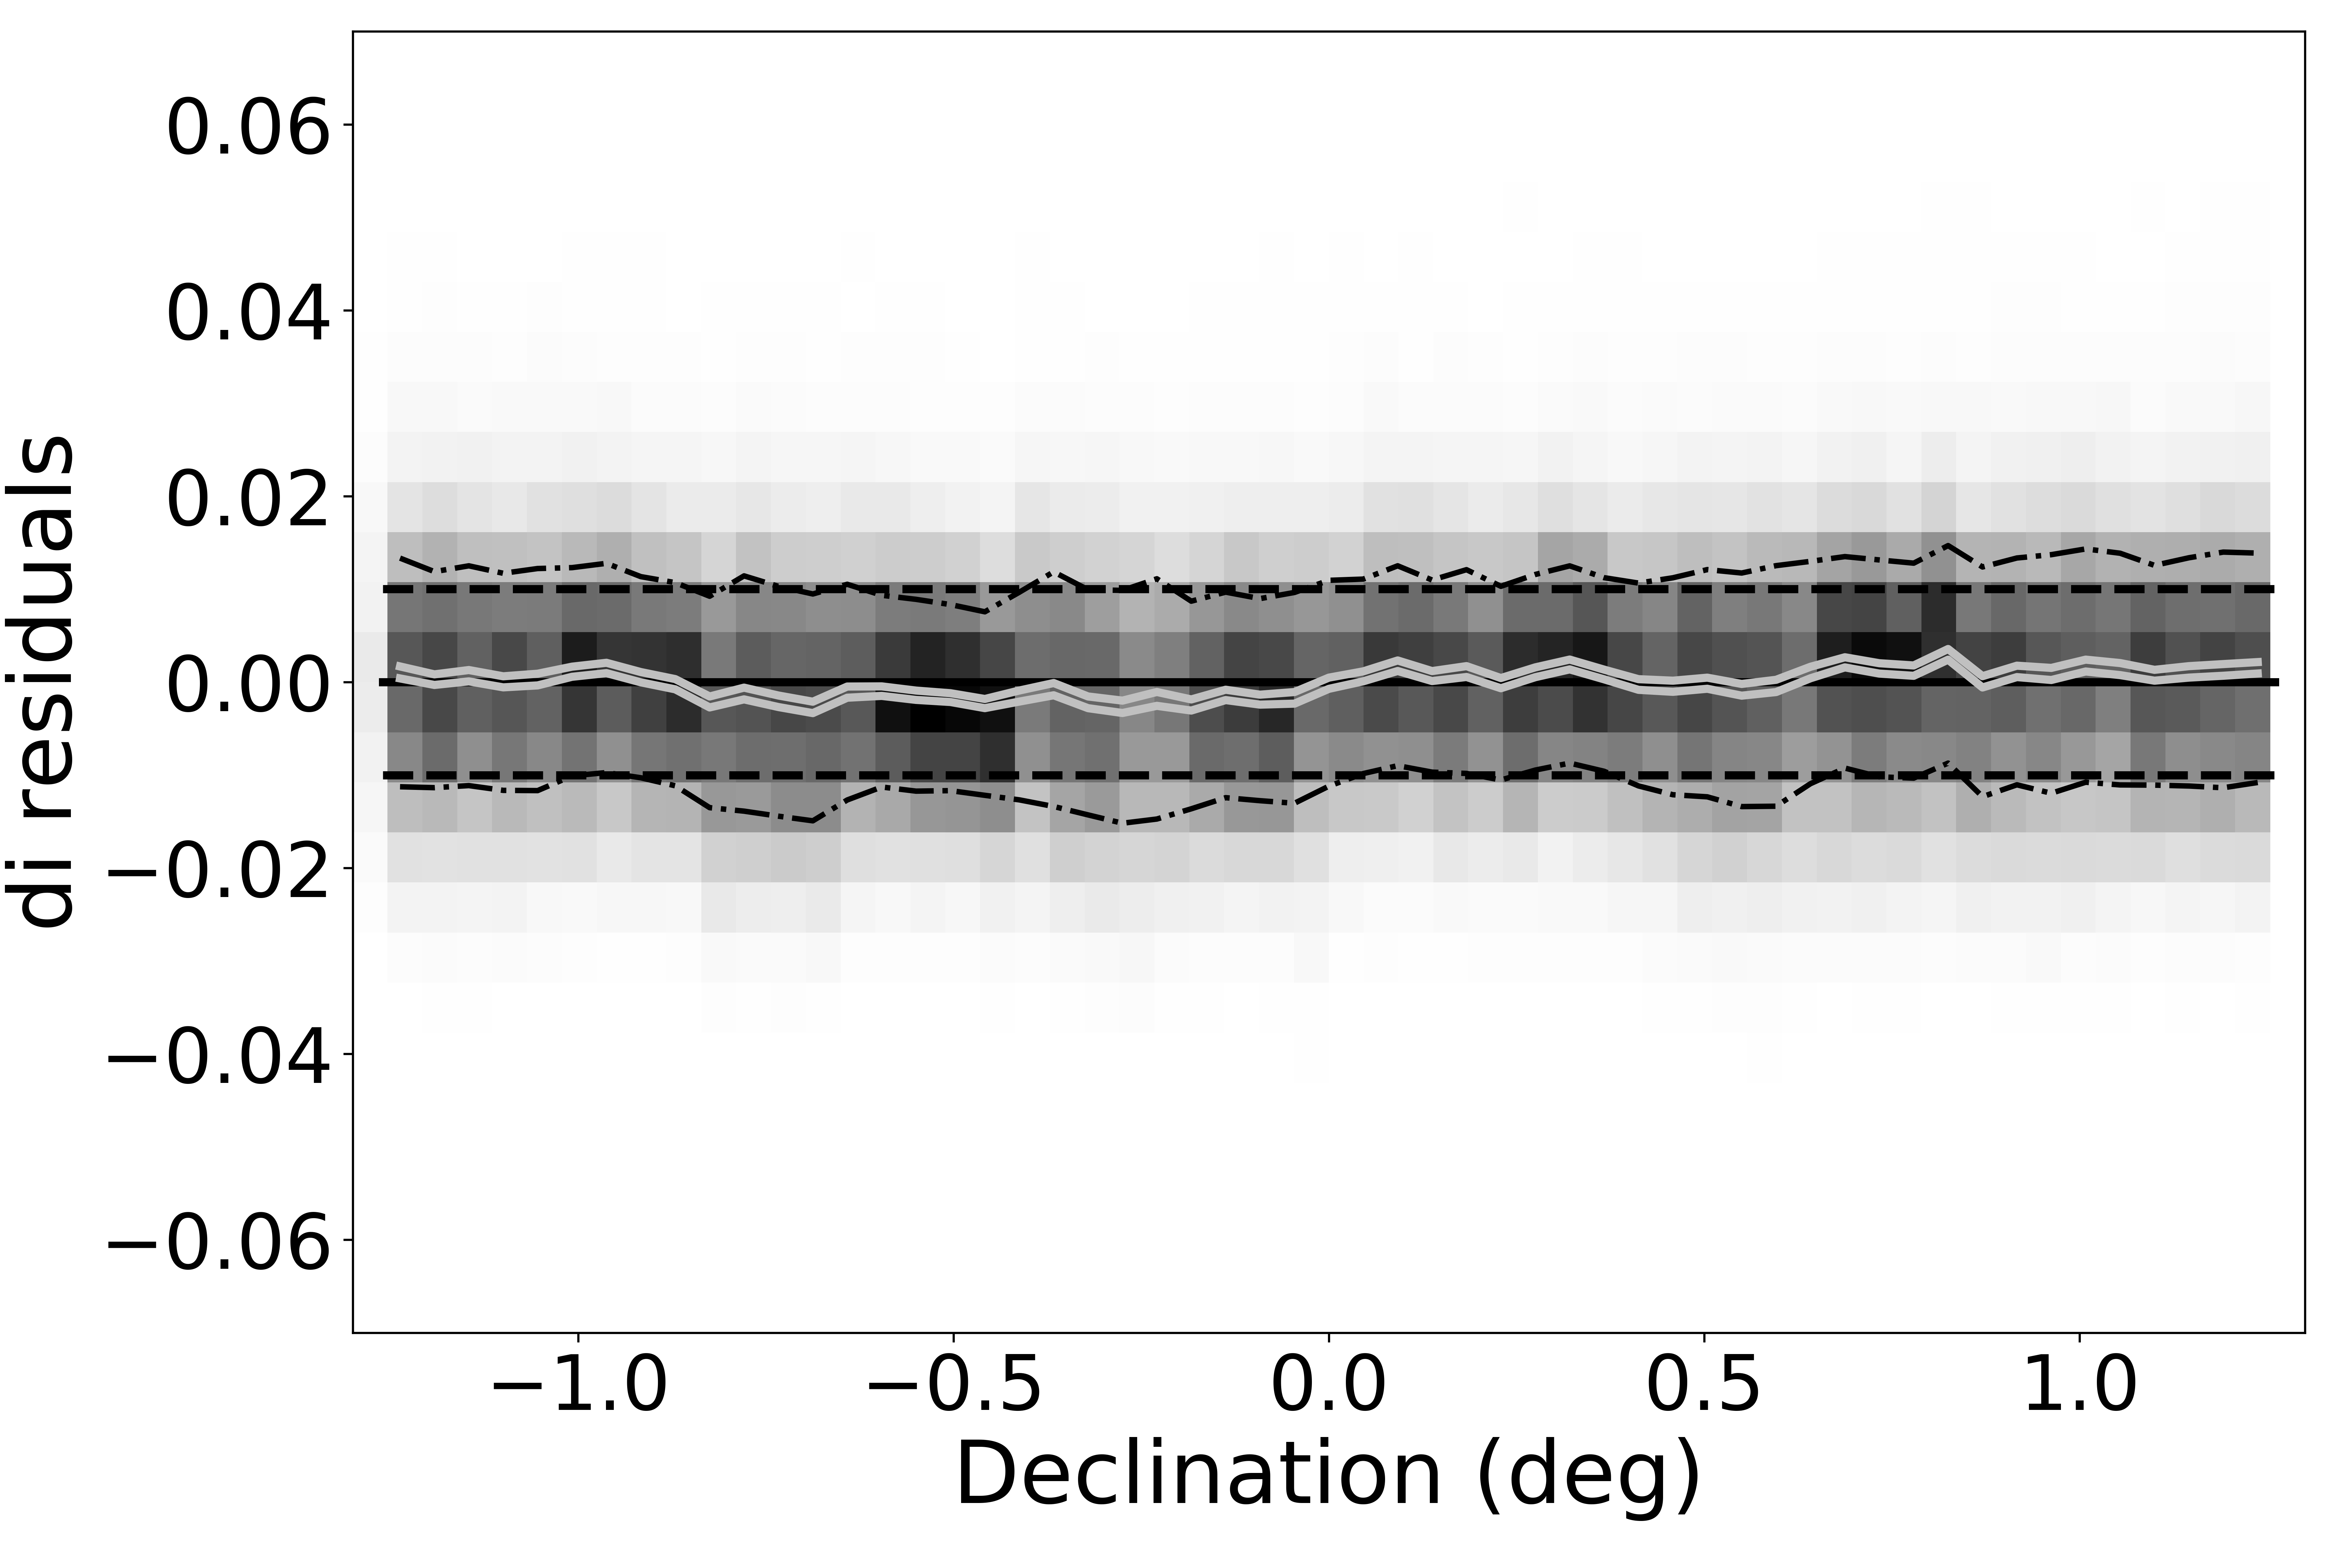
\includegraphics[width=0.45\textwidth]{figures/colorResidDES42bright_di_Dec_Hess.png}
    % \centering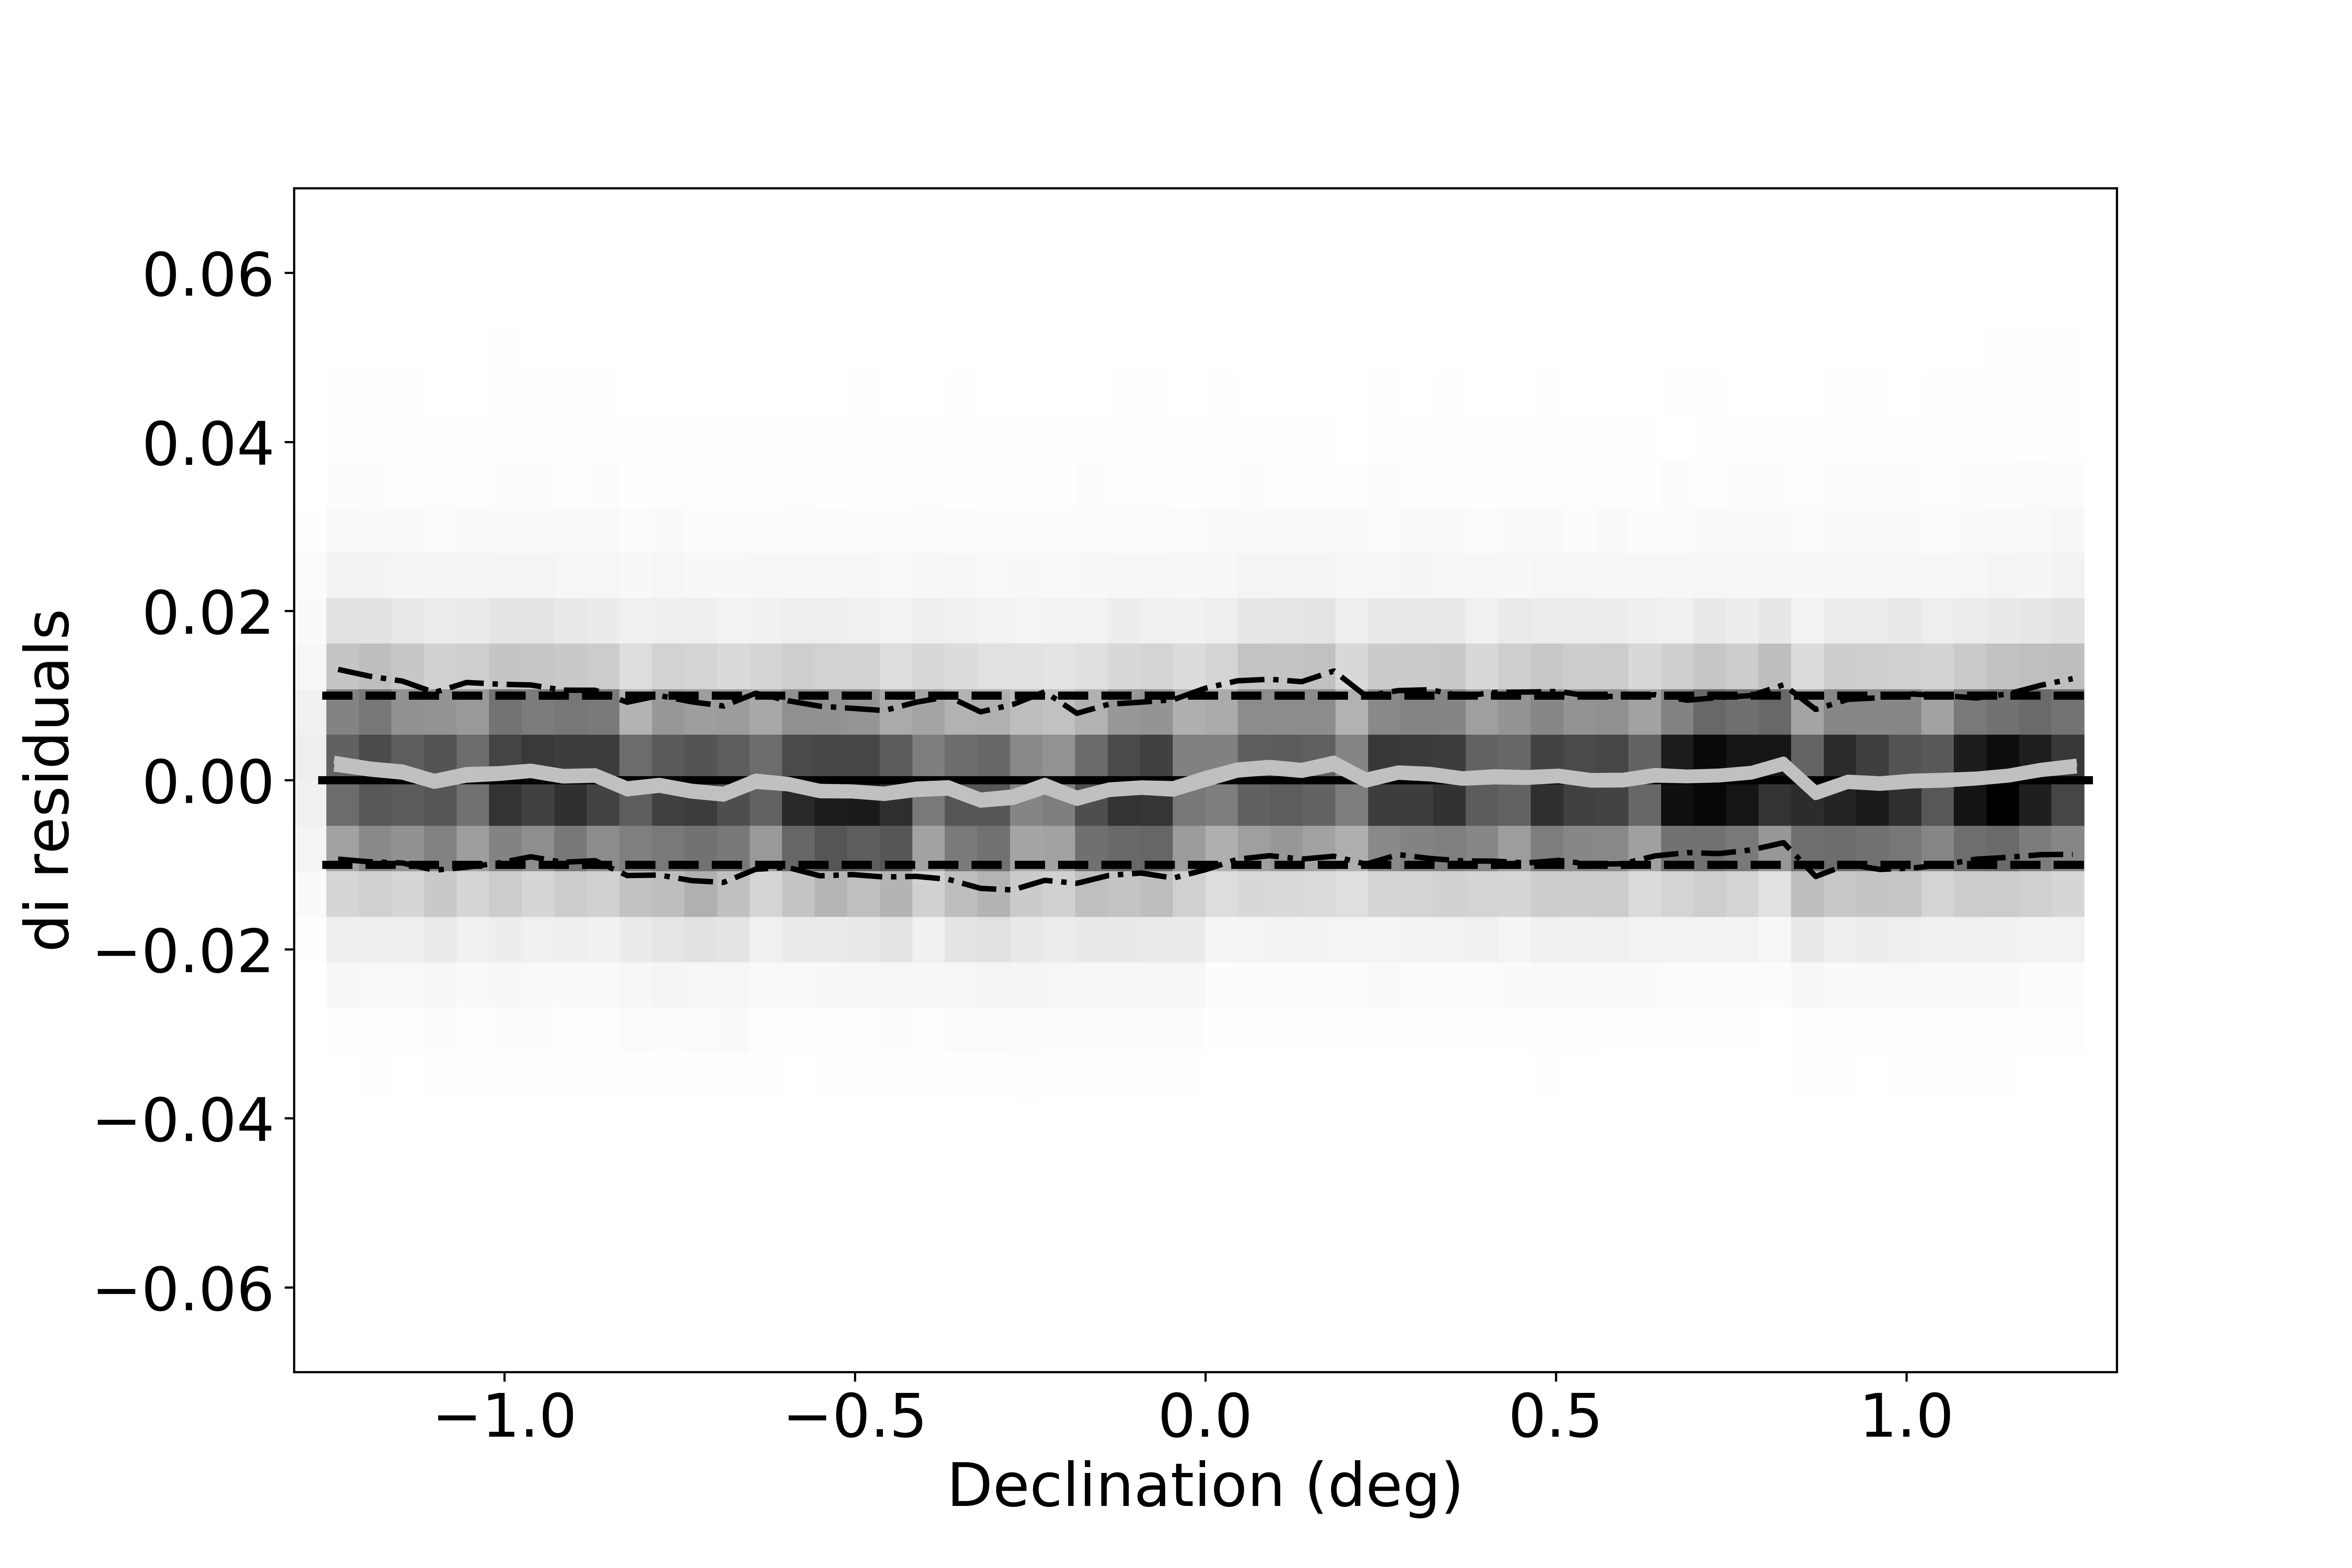
\includegraphics[width=0.45\textwidth]{figures/colorResidPSbright_di_Dec_Hess.png}
    \centering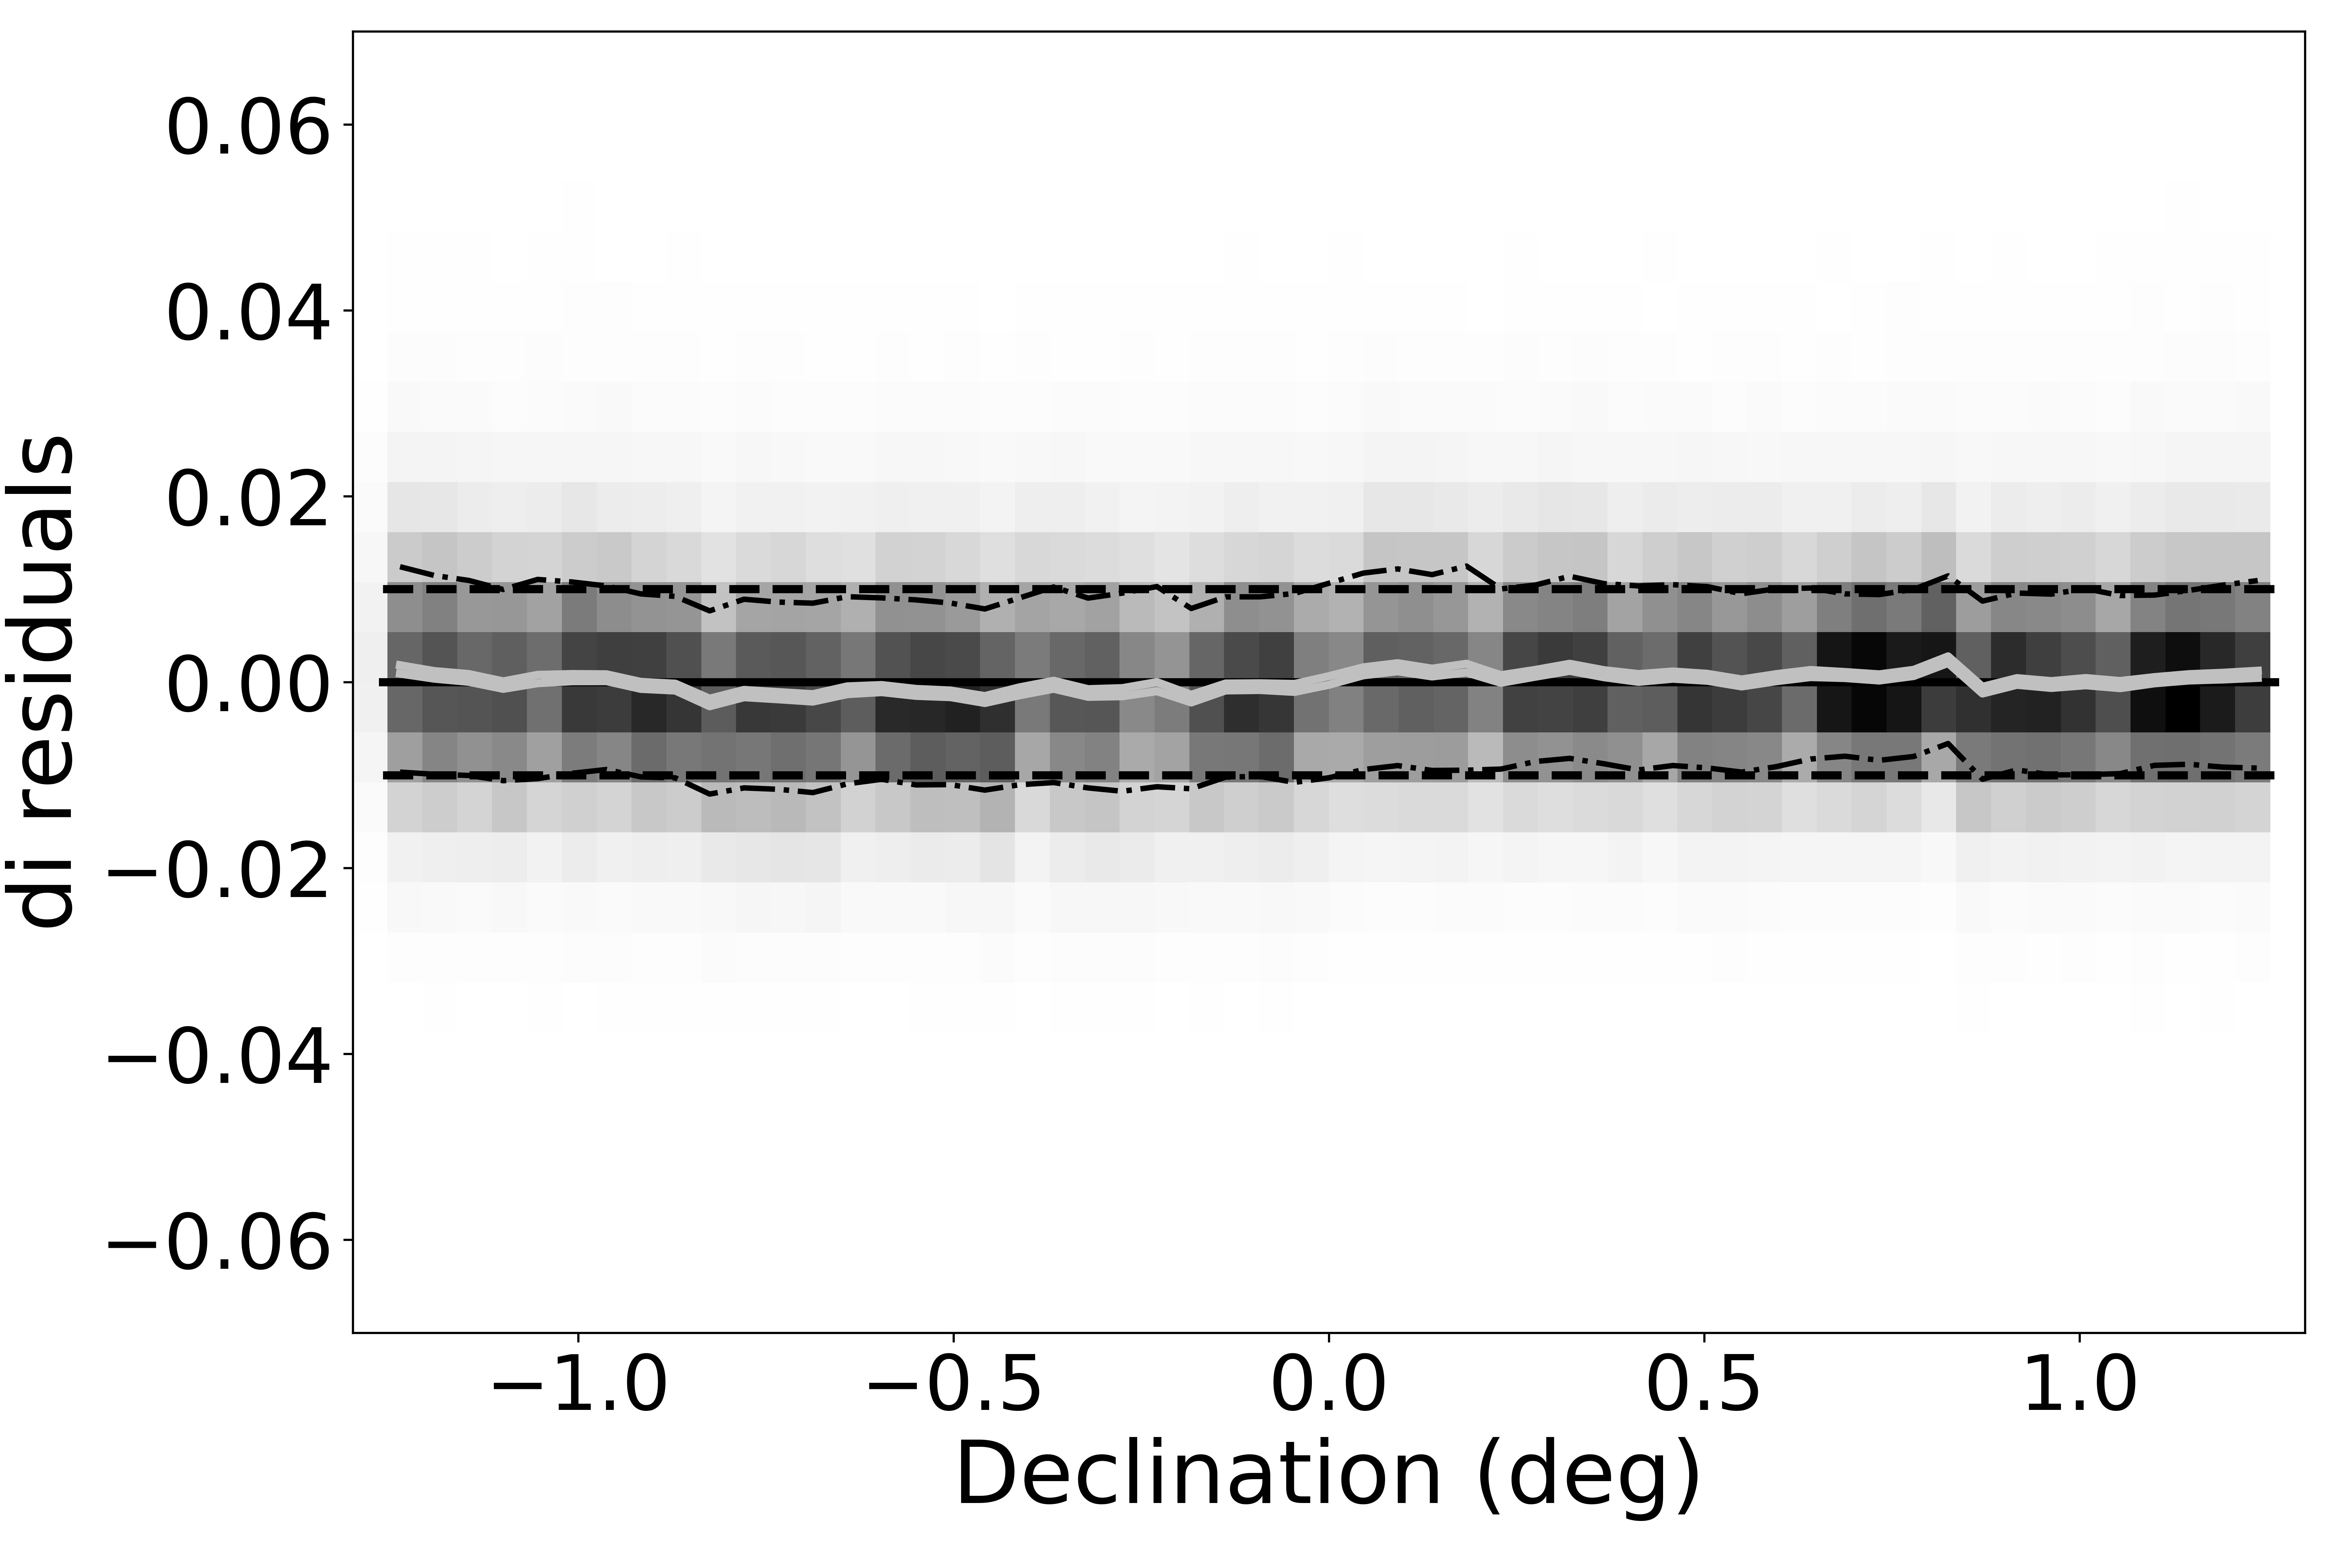
\includegraphics[width=0.45\textwidth]{figures/colorResidPSDR2v42bright_di_Dec_Hess.png}
    \centering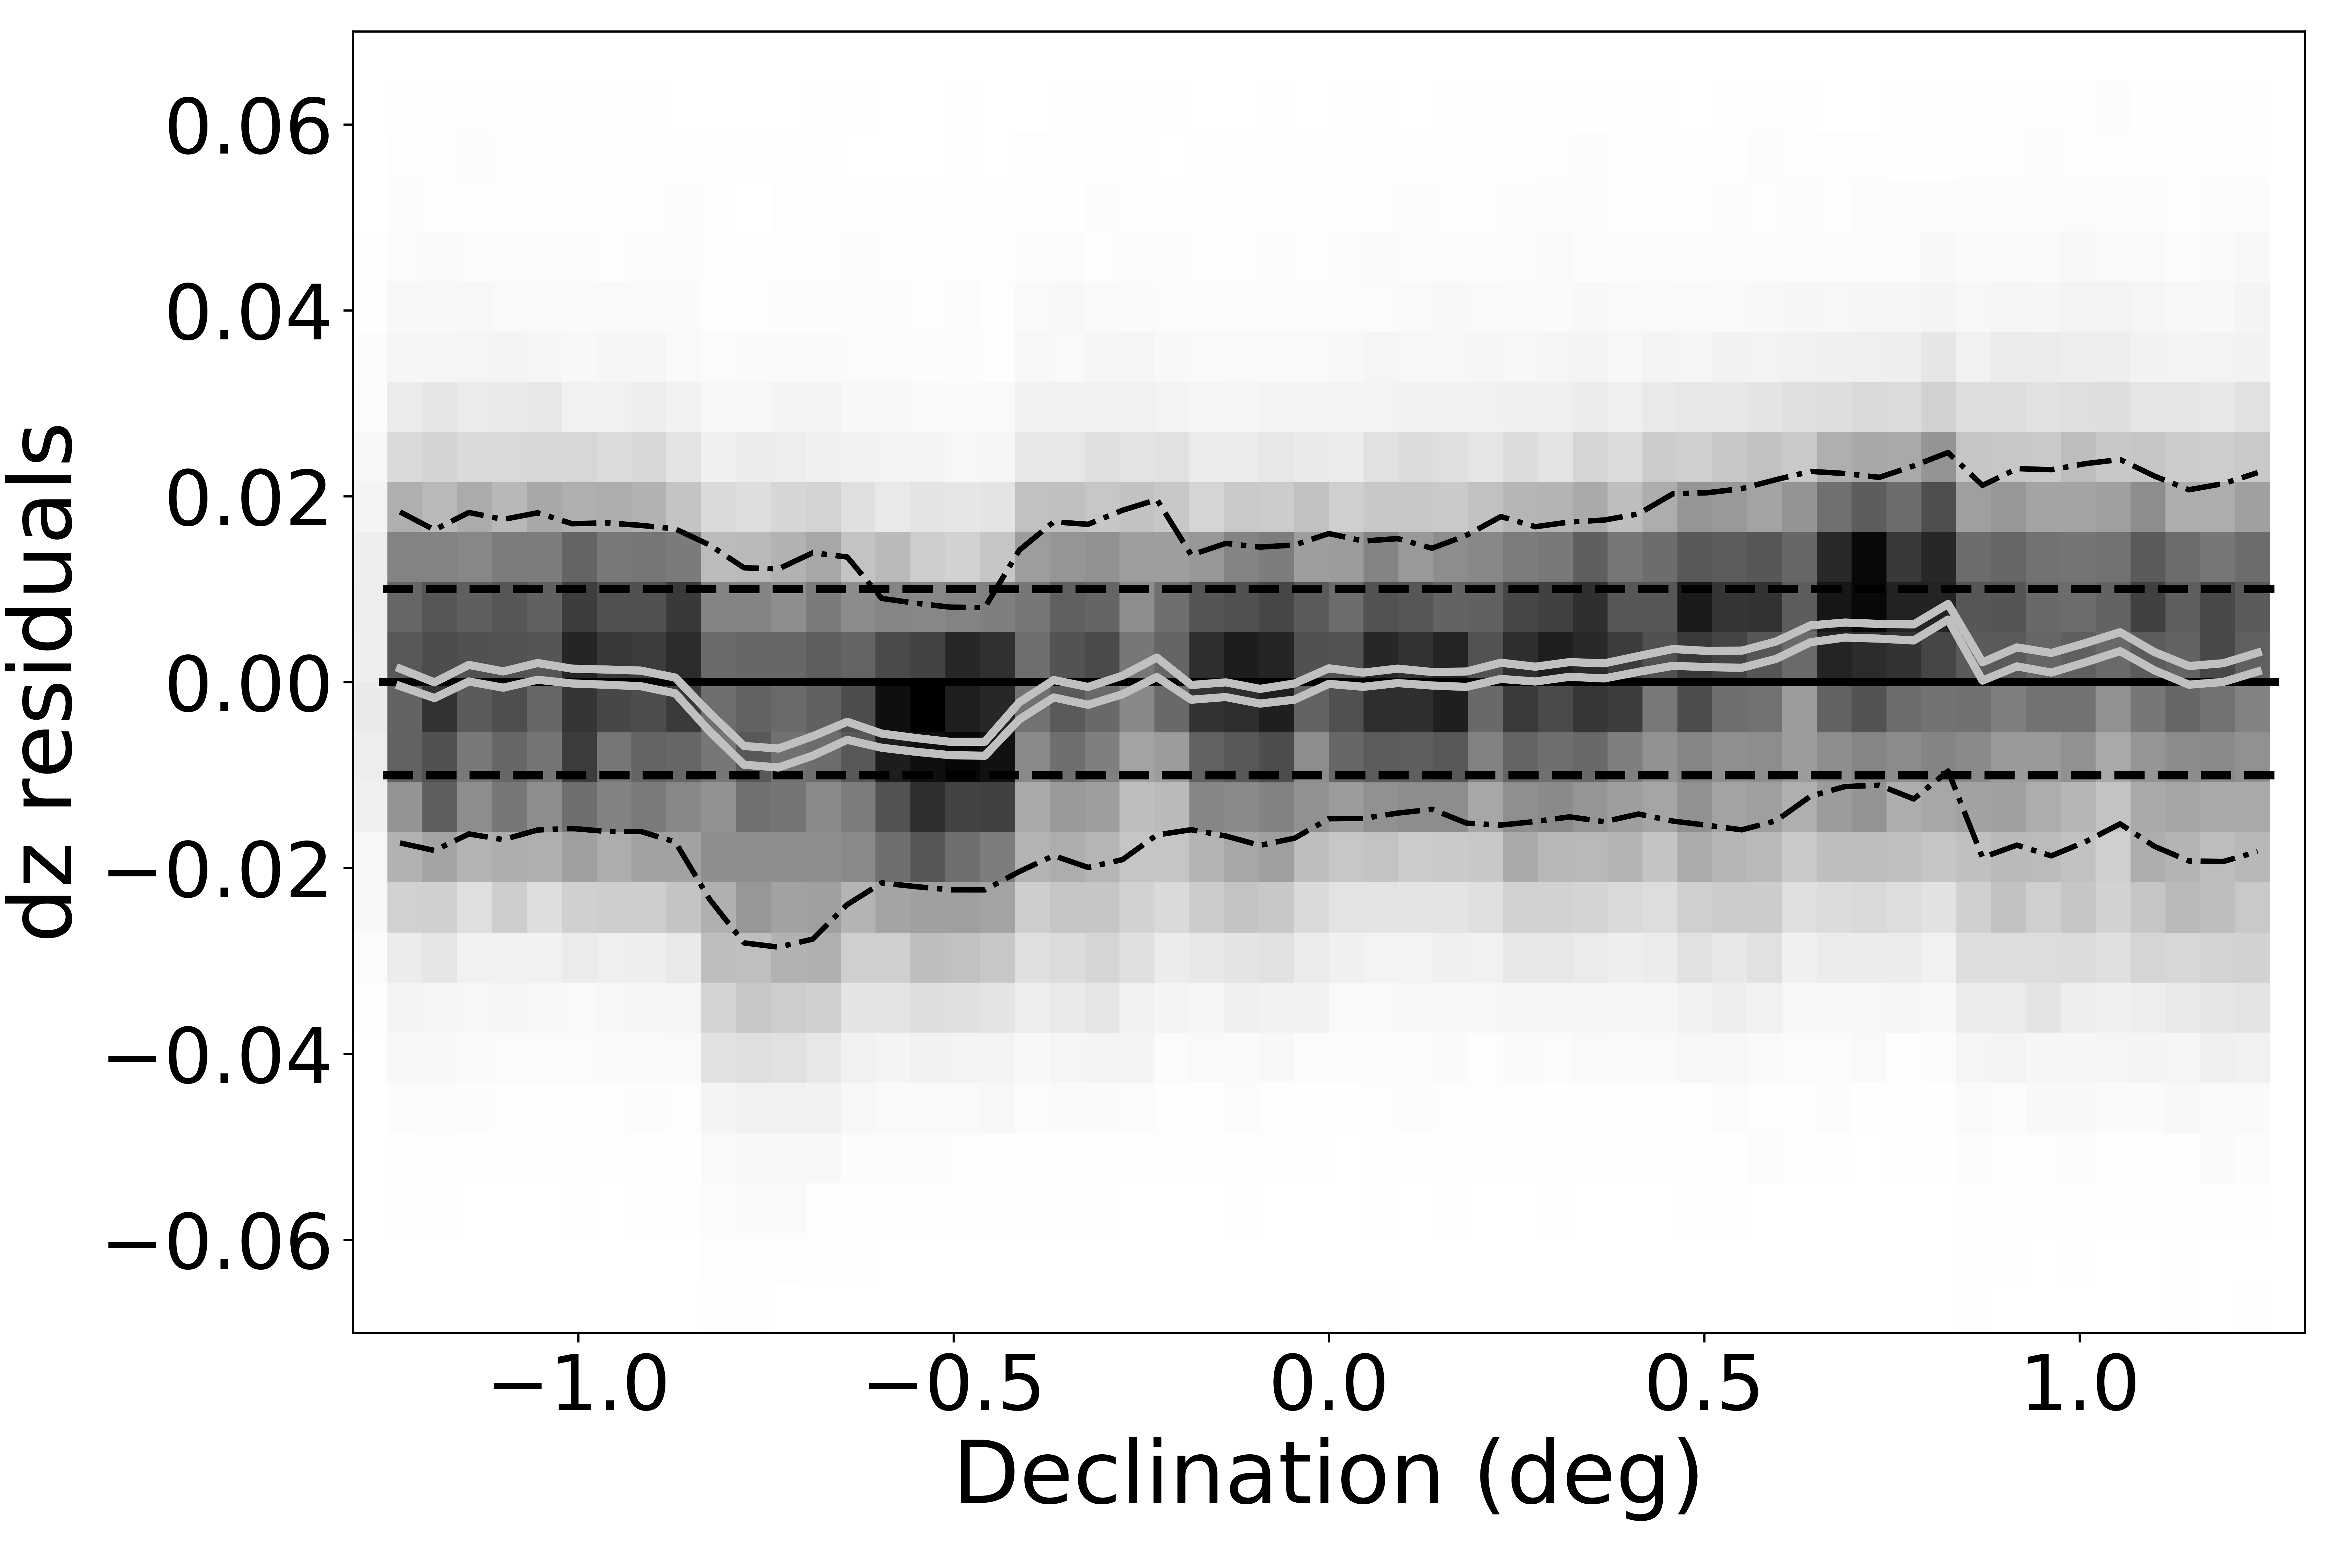
\includegraphics[width=0.45\textwidth]{figures/colorResidDES42bright_dz_Dec_Hess.png}
   %  \centering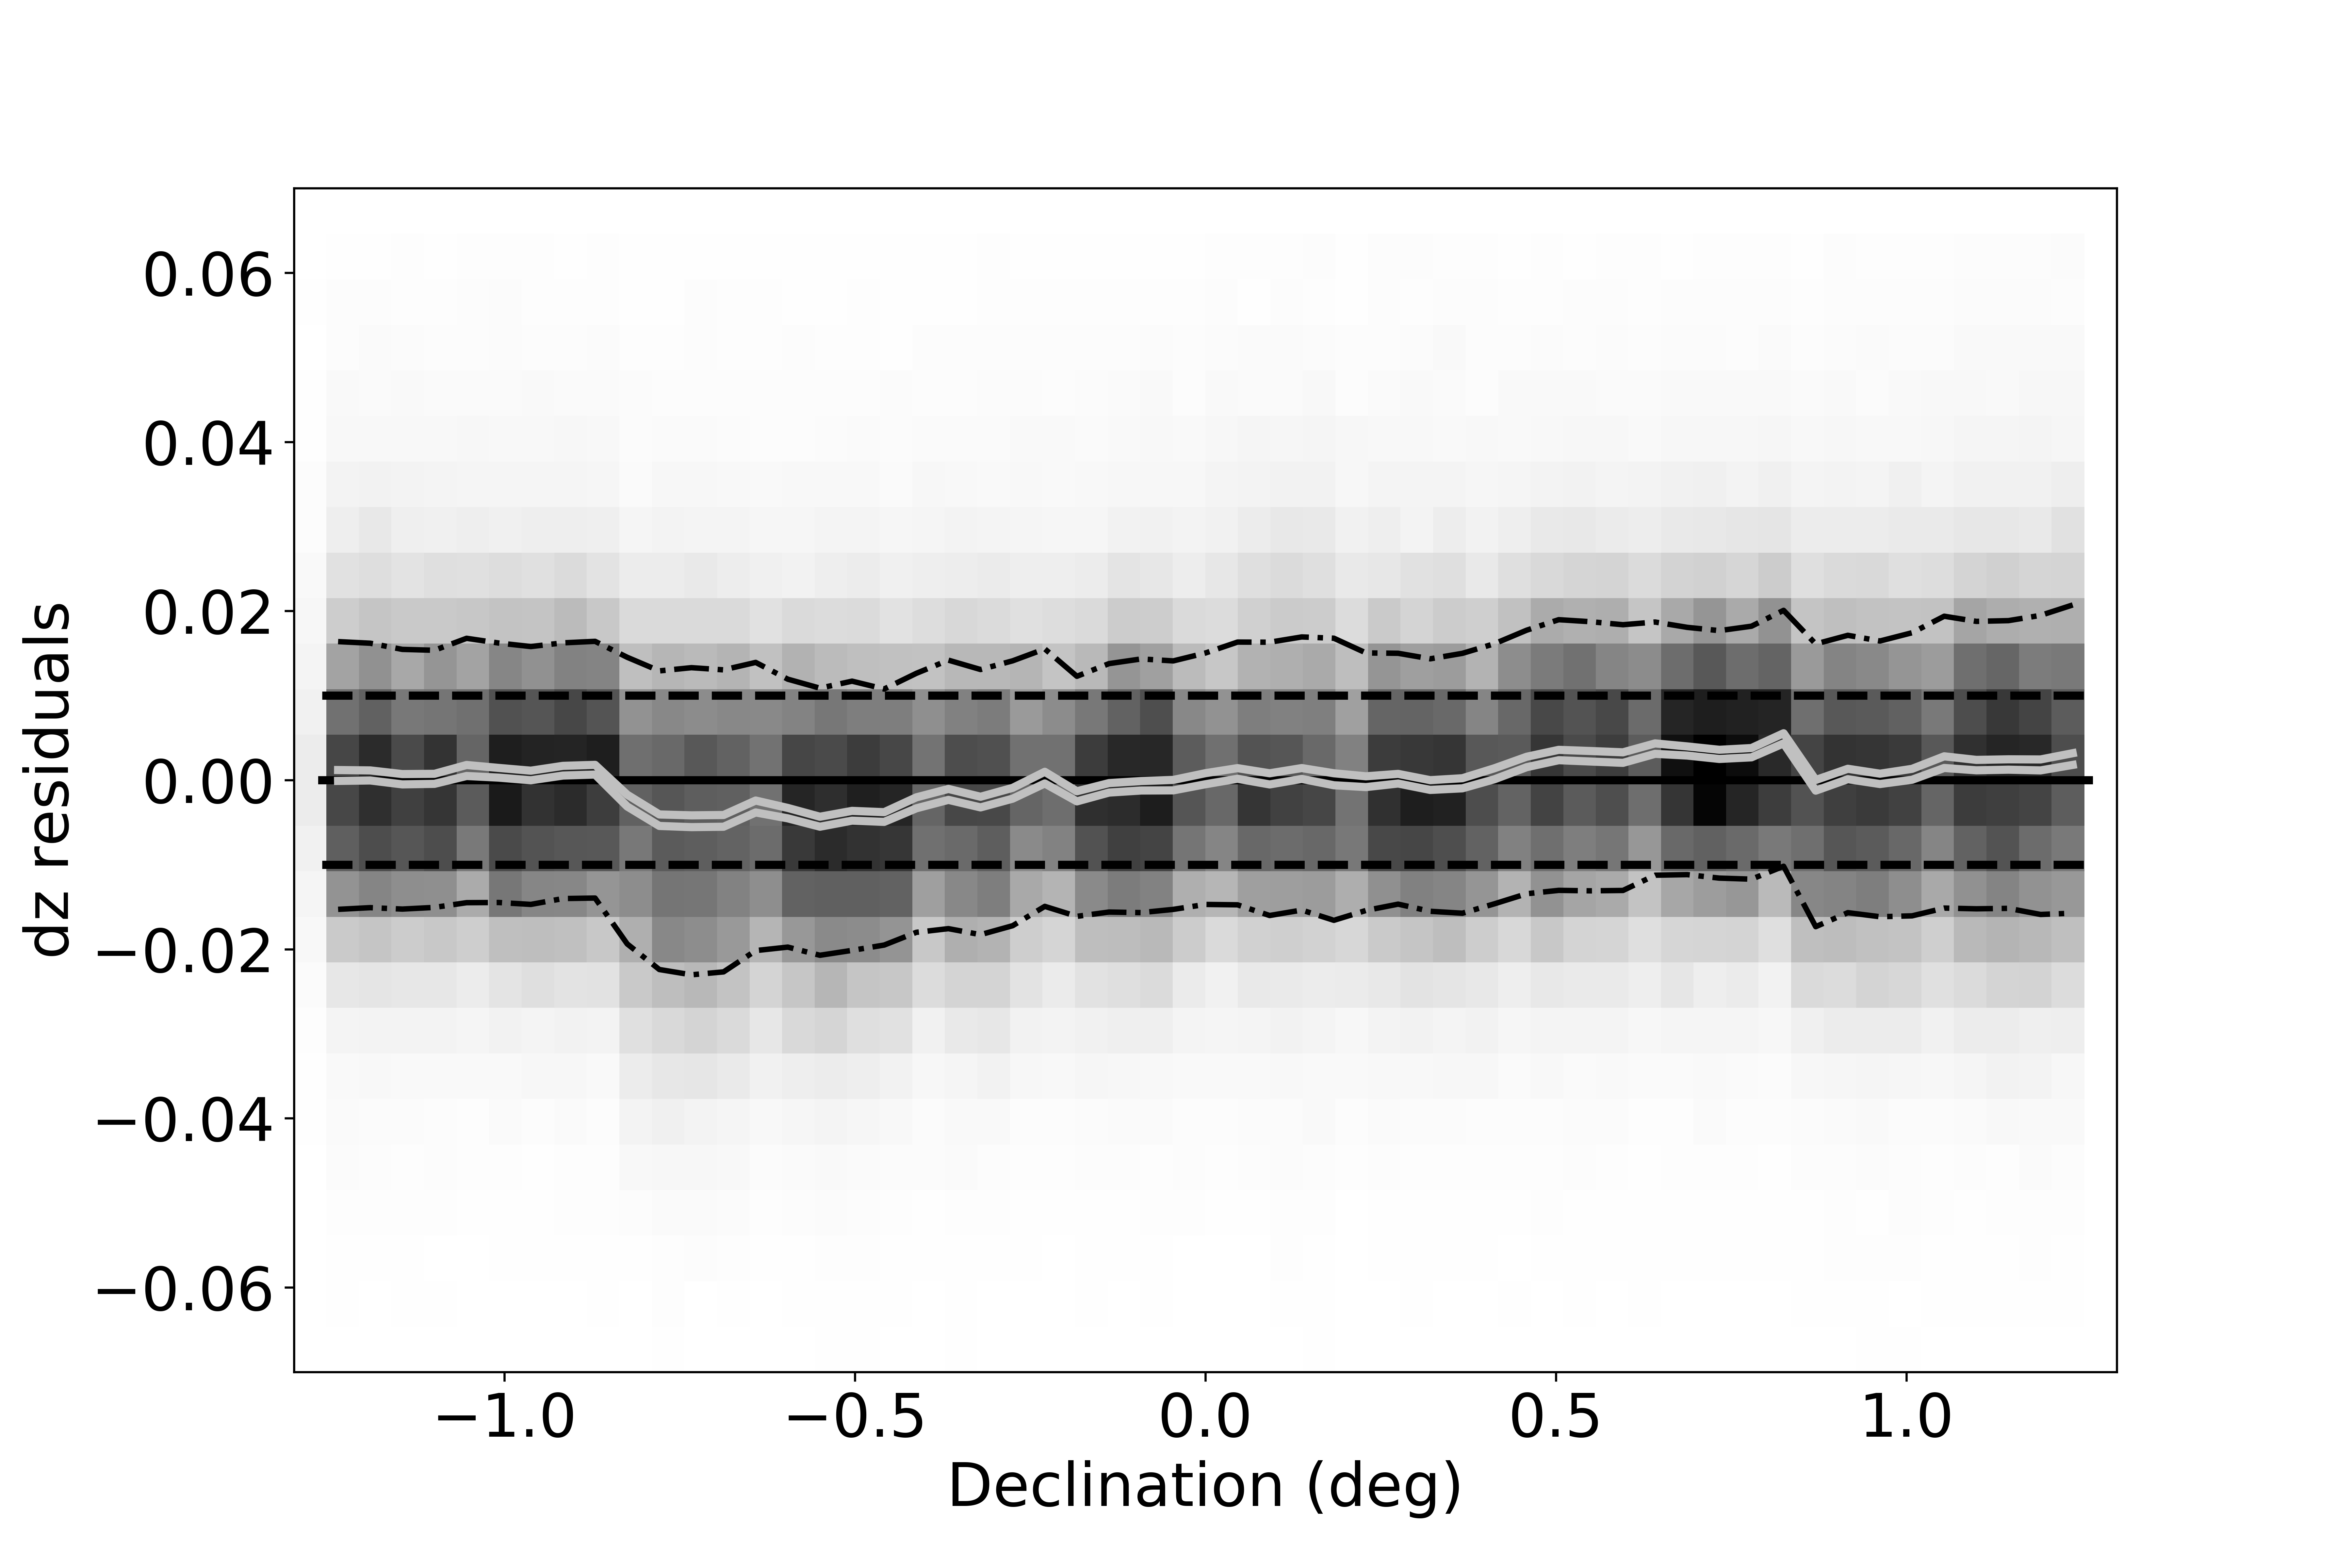
\includegraphics[width=0.45\textwidth]{figures/colorResidPSbright_dz_Dec_Hess.png}
    \centering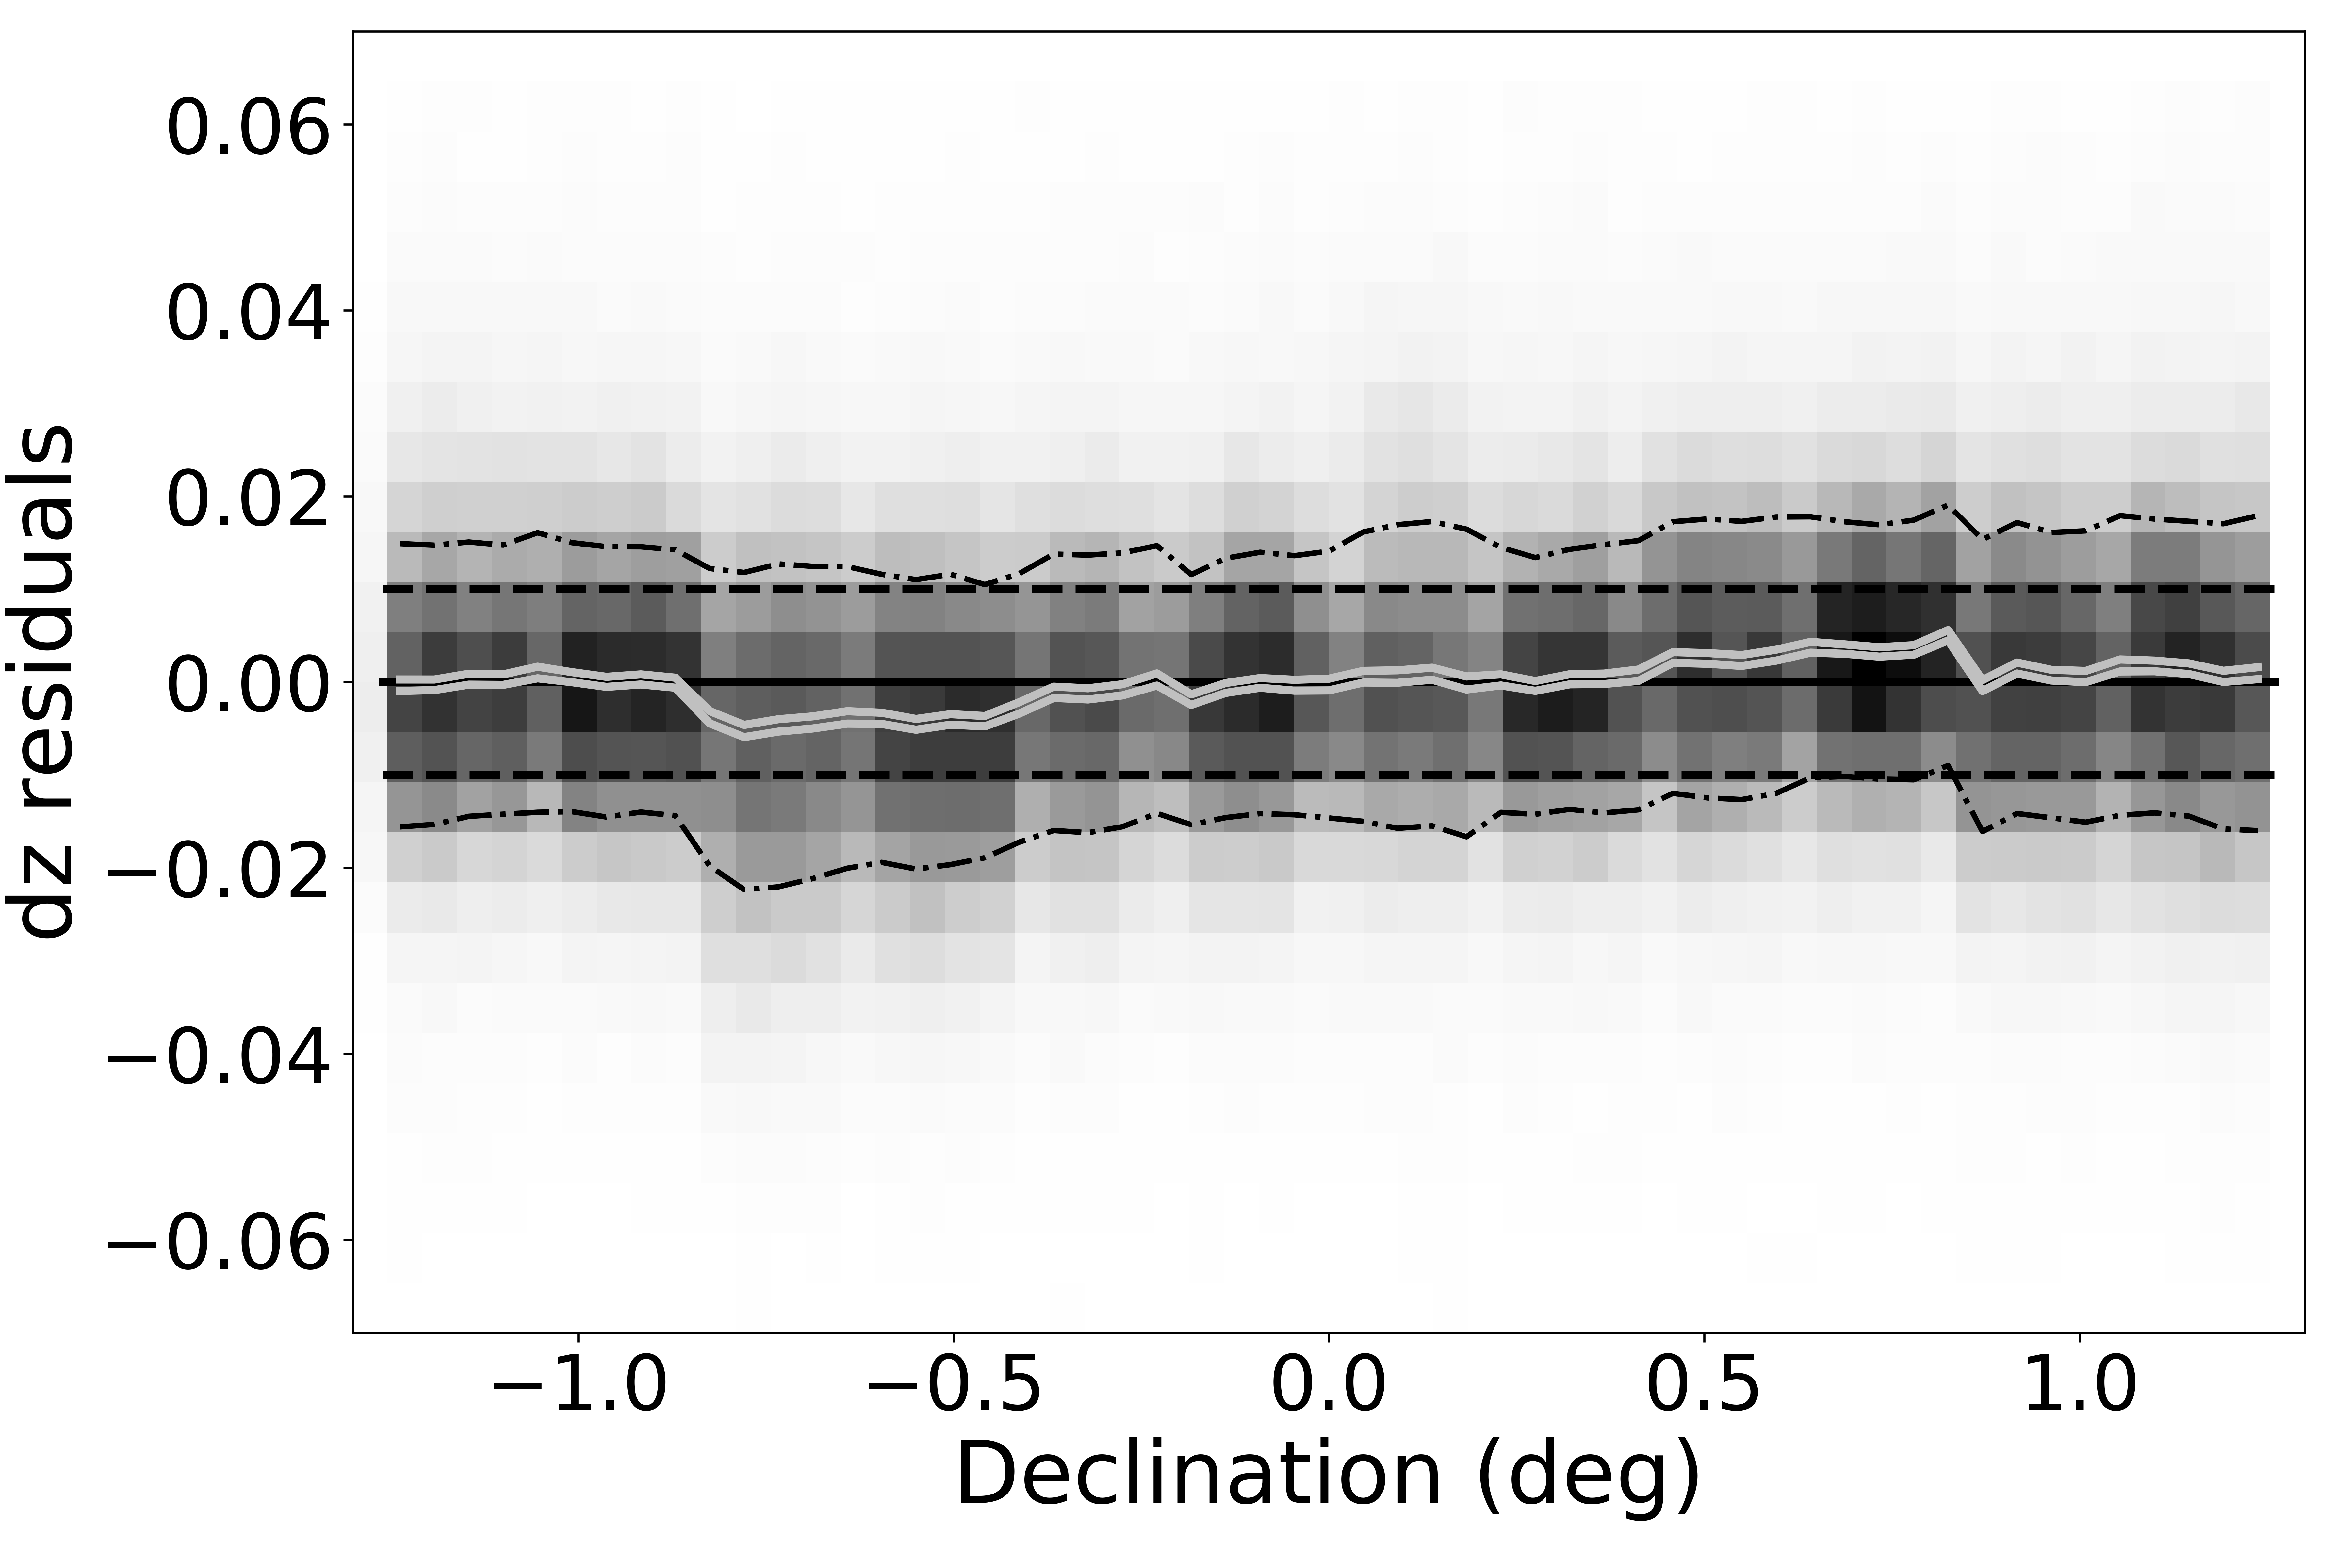
\includegraphics[width=0.45\textwidth]{figures/colorResidPSDR2v42bright_dz_Dec_Hess.png}
\caption{Analogous to Figure~\ref{fig:DESPSRA}, except that magnitude differences
are binned by Declination.}
\label{fig:DESPSDec}
\end{figure*}

\begin{figure*}
    \centering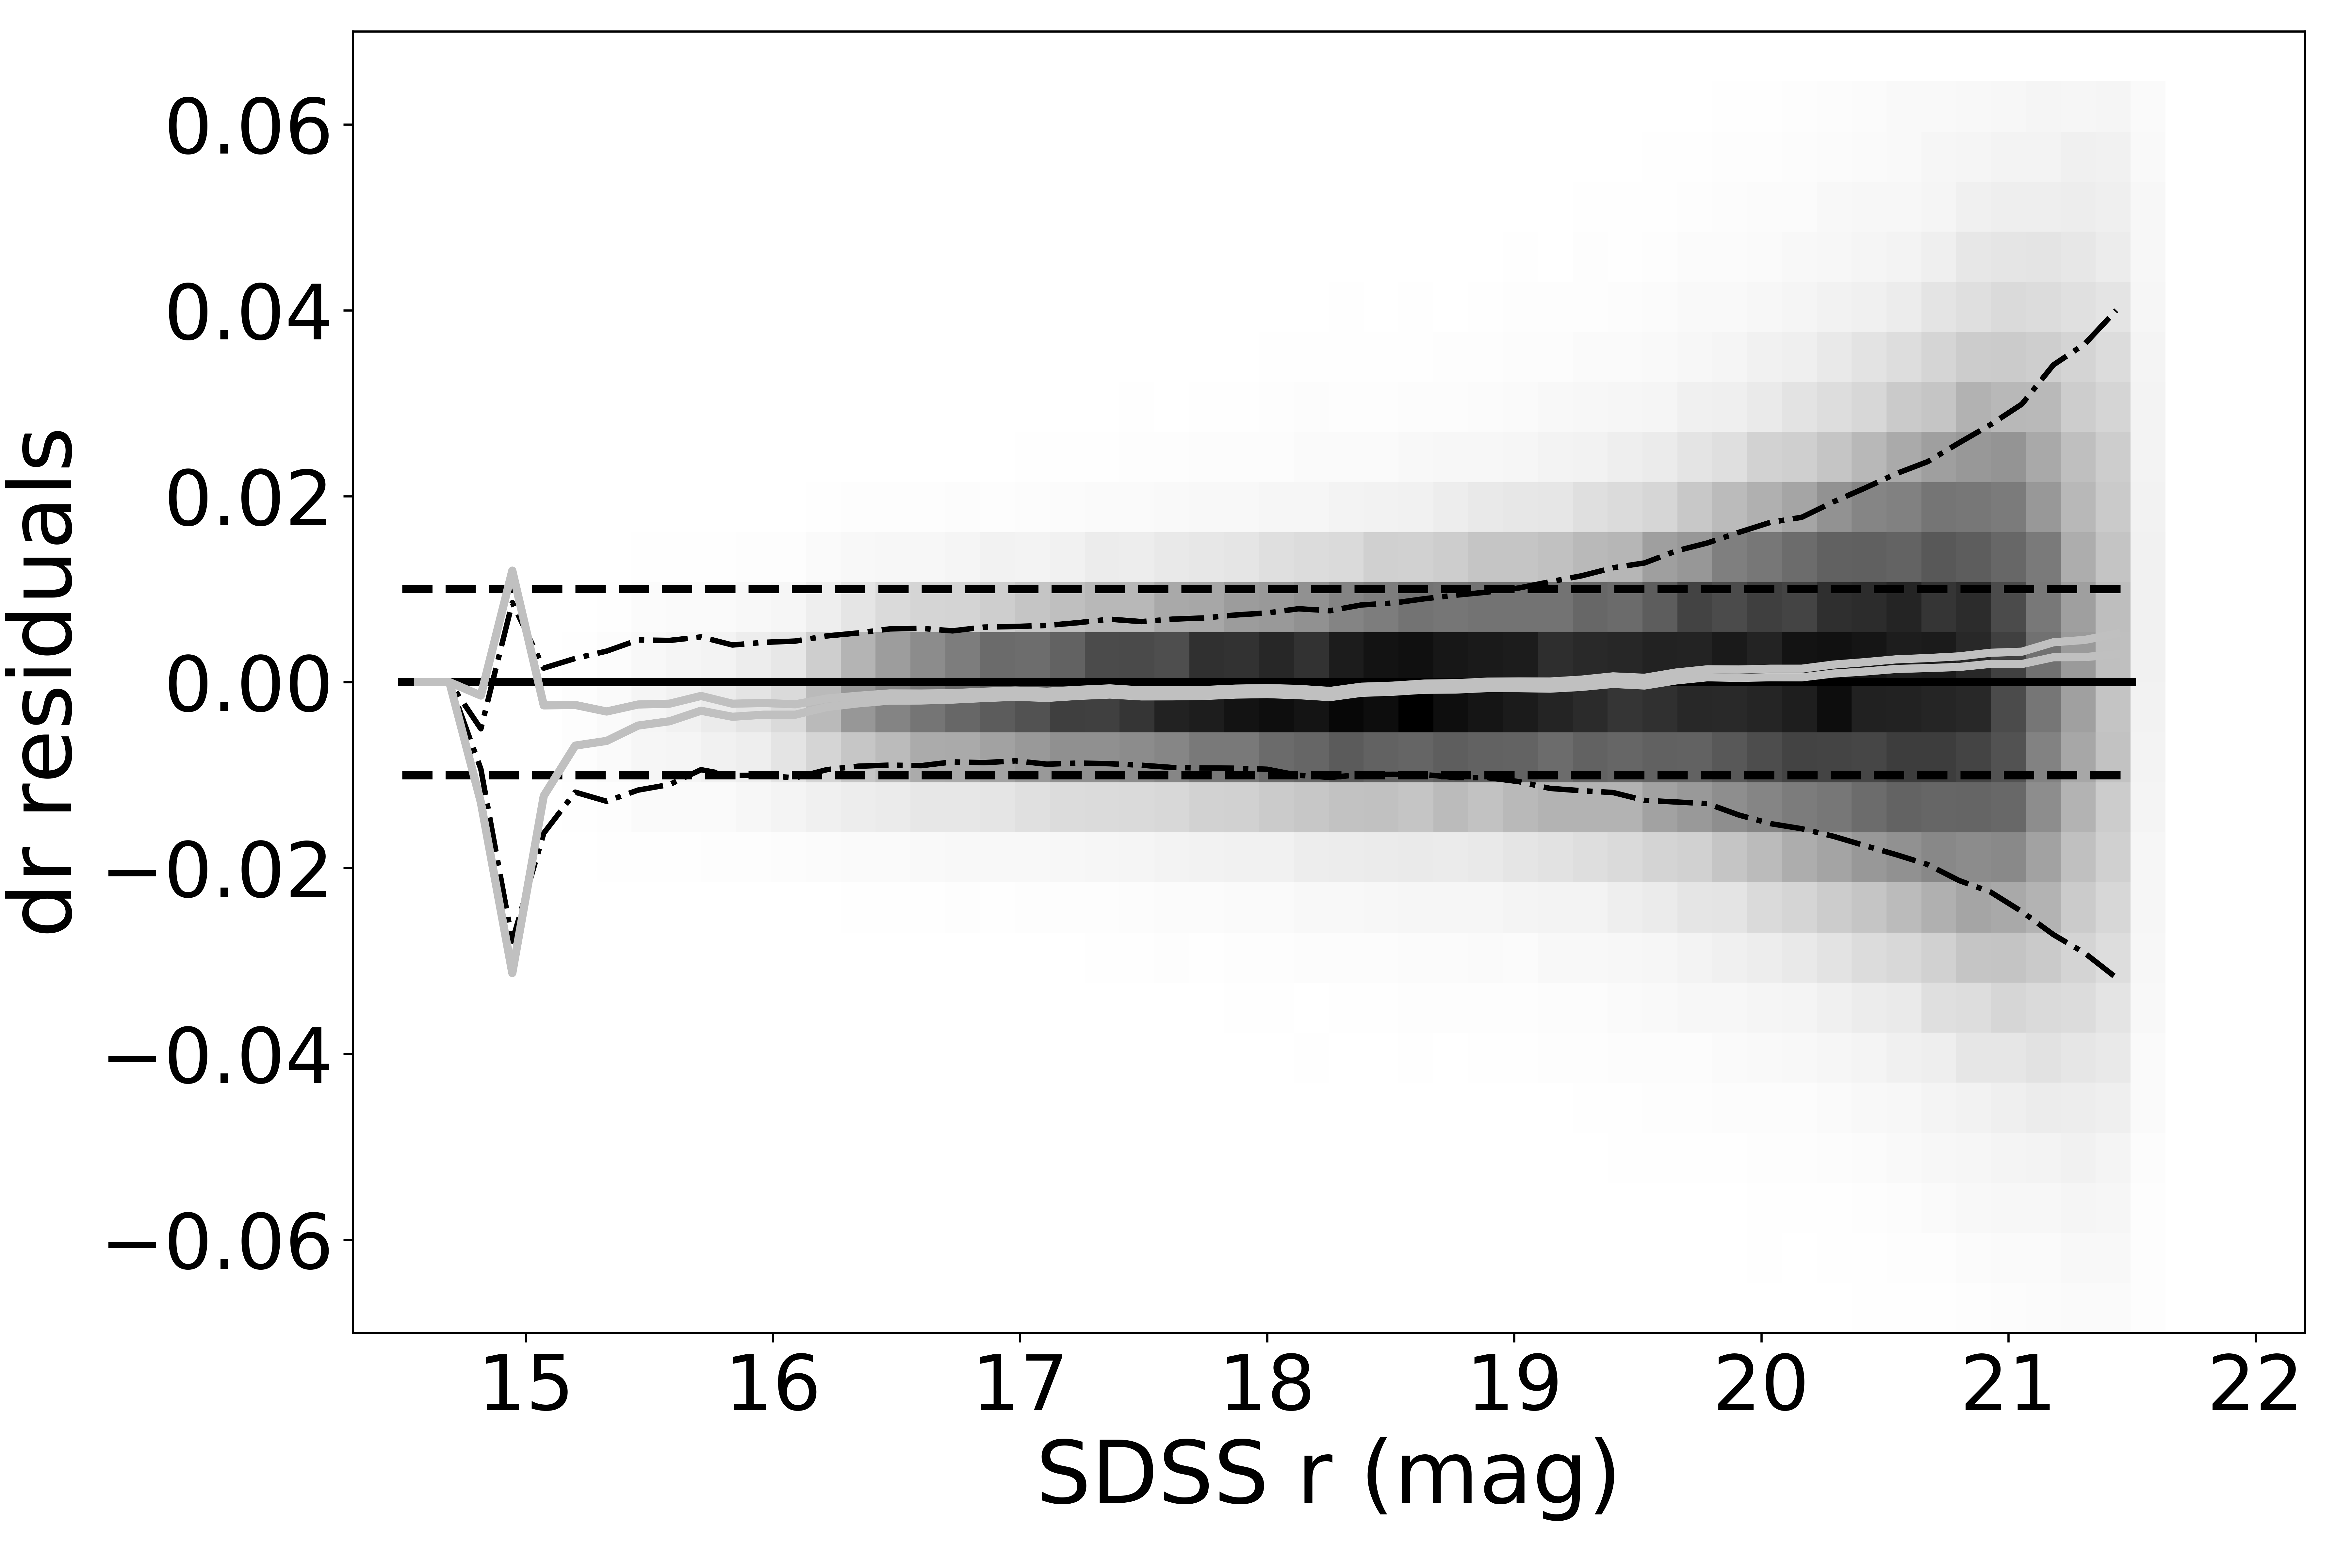
\includegraphics[width=0.45\textwidth]{figures/colorResidDES42_dr_rmag_Hess.png}
    \centering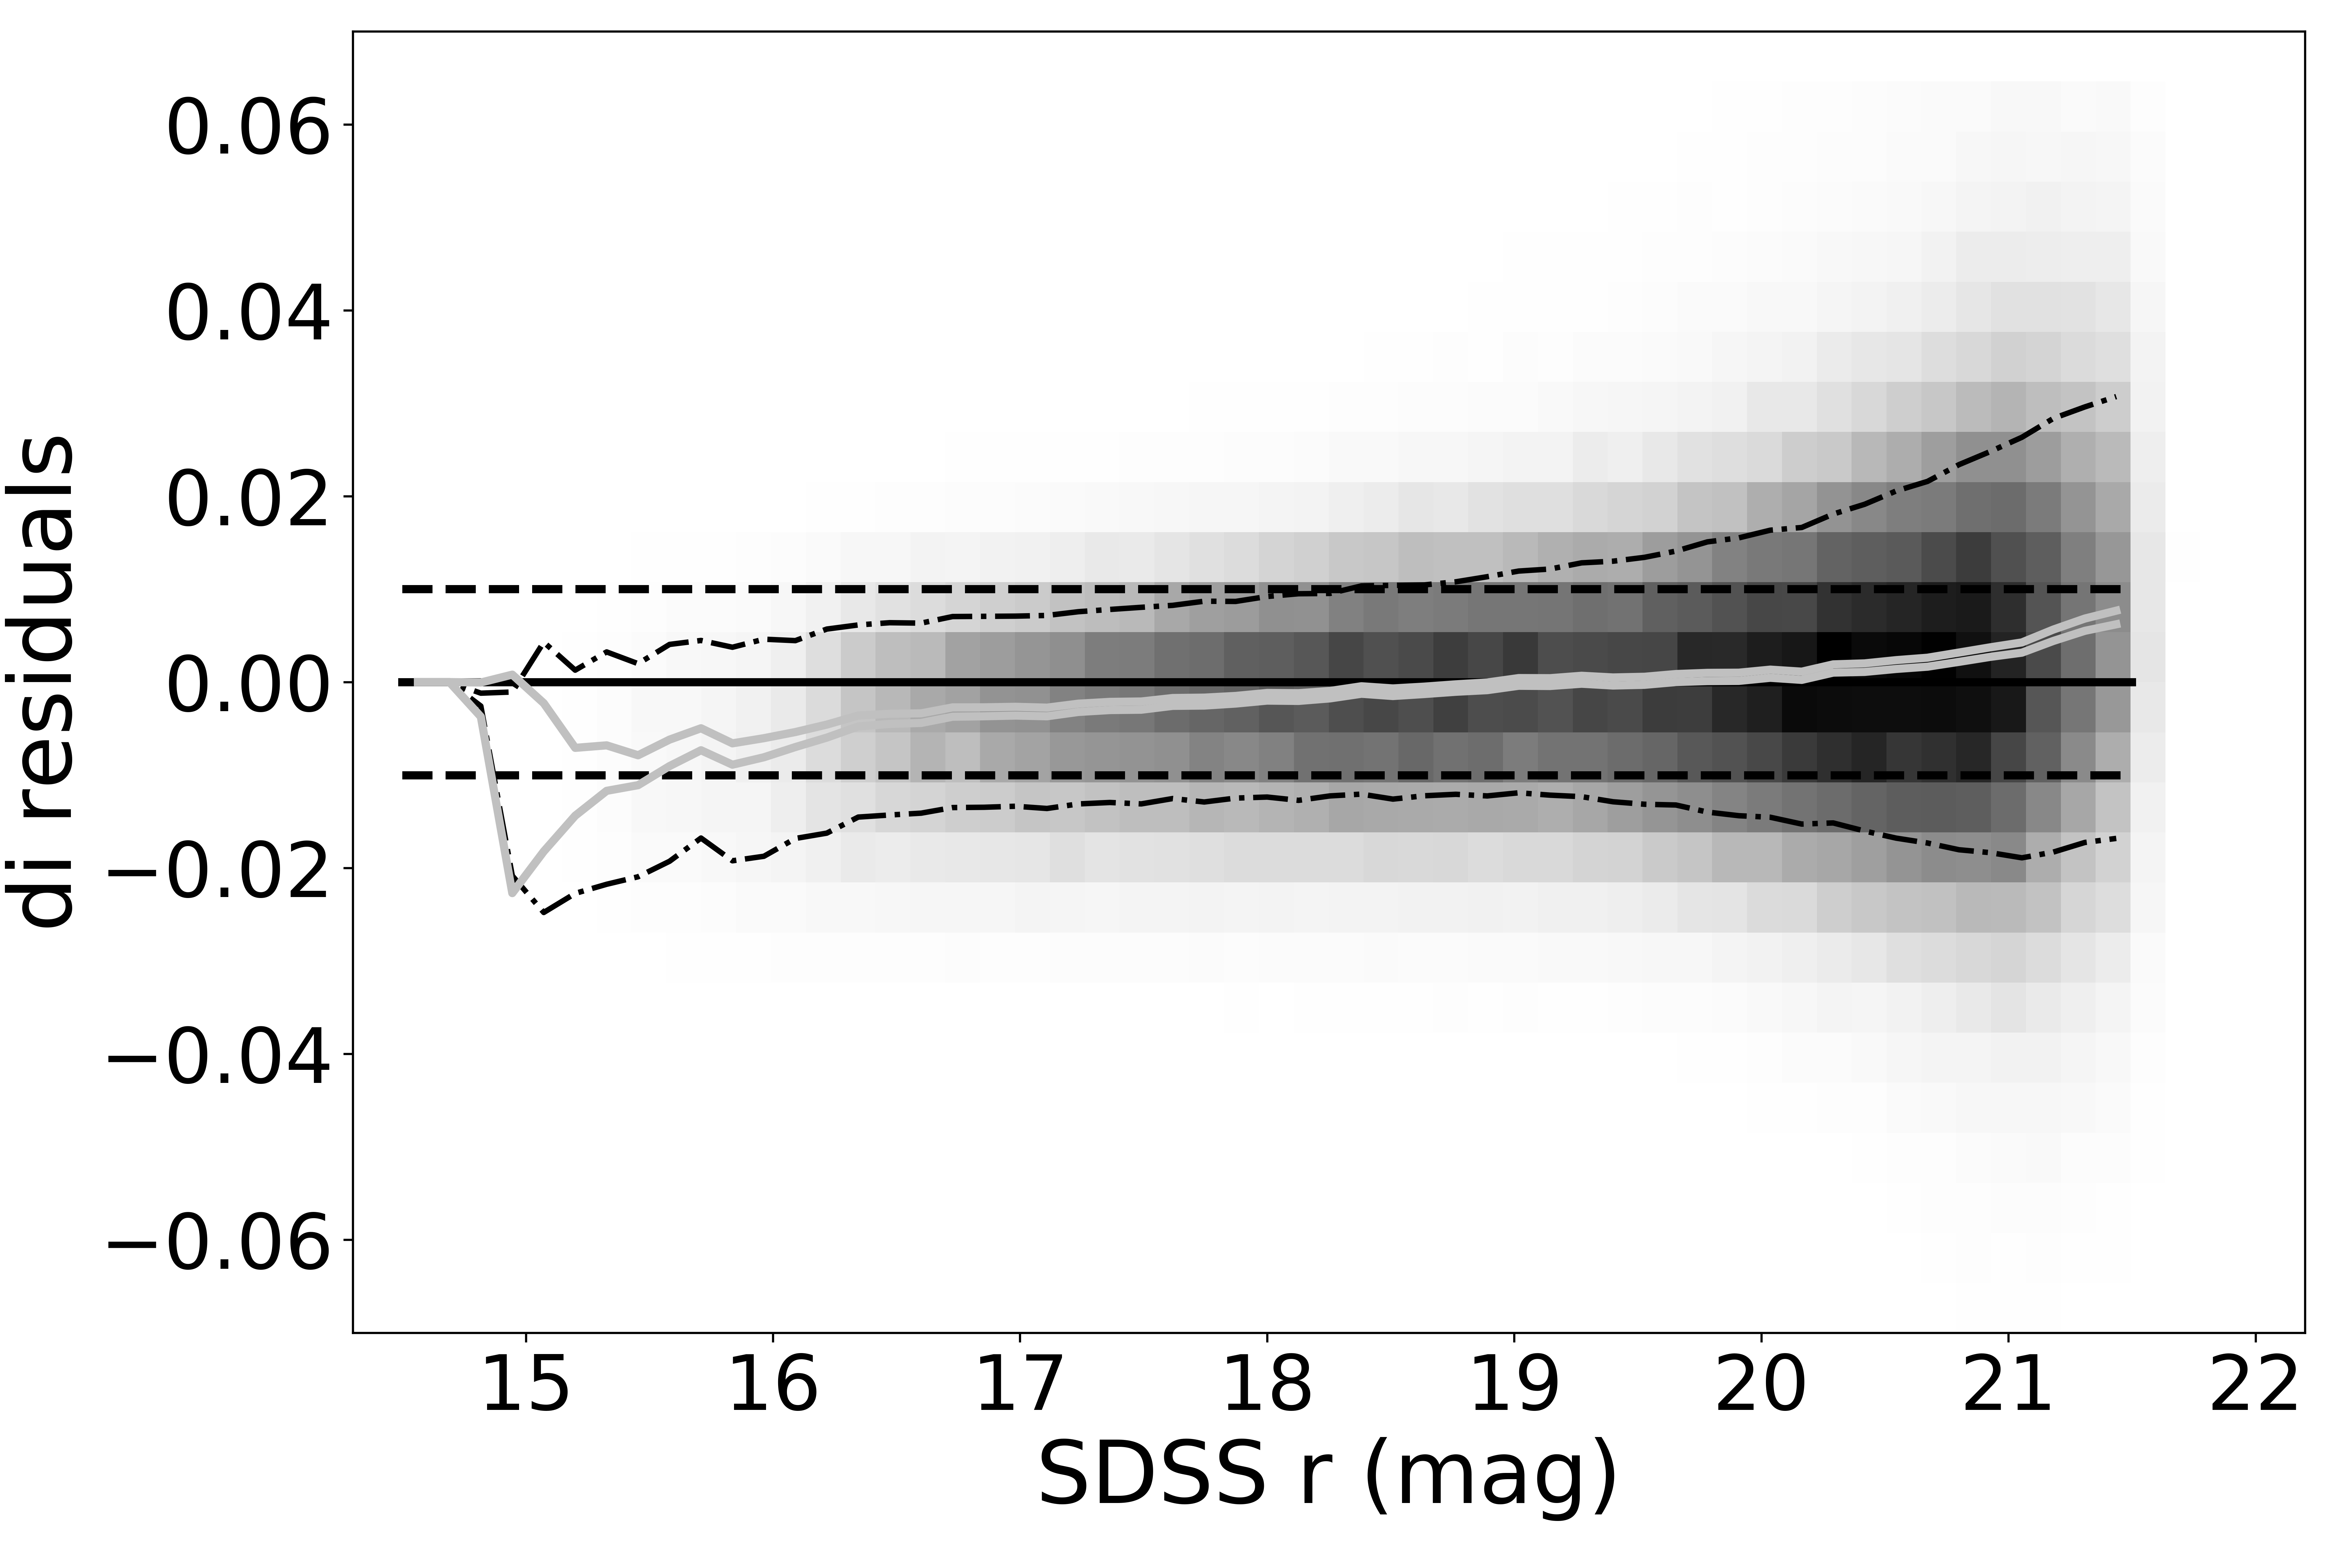
\includegraphics[width=0.45\textwidth]{figures/colorResidDES42_di_rmag_Hess.png} 
\caption{A comparison of the magnitude differences between the SDSS v4.2 catalog
and DES catalog, for the $r$ and $i$ bands. Note the very small gradient of the median
residuals between the bright and faint ends: about 3-4 millimag and thus much smaller
than $\sim$20 millimag when comparing to Gaia magnitudes (see Figure~\ref{fig:gaiaJump}).} 
\label{fig:drVSr}
\end{figure*}

%%%%%%%%%%%%%%%%%%%%%%%%%%%%%%%%%%%%%%%%%


\subsection{Comparison of the new v4.2 SDSS catalog and $u$ band data from the CFIS catalog  \label{sec:CFIStest}} 

The comparison of the new SDSS catalog with the DES and Pan-STARRS catalogs in the previous
section did not include the $u$ band. To assess the quality of $u$ band zeropoint calibration, 
we use the CFIS catalog (see Section~\ref{ssec:cfis}). The CFIS $u$ band photometry was 
calibrated using a combination of the SDSS, Pan-STARRS and GALEX UV data. Given that
we recalibrated the new SDSS catalog using Gaia data, it should not matter for this comparison that SDSS data were used in calibration of the CFIS catalog. Nevertheless, this should be kept in mind while interpreting the results presented in this section.  We also note that the transmission curve of the MegaCam $u$ band filter used for the CFIS survey differs from that of the SDSS $u$ band filter\footnote{https://www.cadc-ccda.hia-iha.nrc-cnrc.gc.ca/en/megapipe/docs/filt.html}. However, we there are no noticeable differences seen in the magnitude comparisons between the two catalogs presented here. 
%Nevertheless, the results of this section should be treated with caution. 

A comparison for about 150,000 sufficiently bright stars ($r<20$), with colours matching the main sequence ($1.0 <u-g < 2.1$)  is illustrated in Figure~\ref{fig:CFIS}. The binned median scatter for Declination direction is 
5.7 millimag with systematic differences of up to about 0.01 mag. The constraints in the R.A. direction 
are noisier, with residuals appearing about twice as large as in the Declination direction. 
These residuals compare favorably to the results of analysis by \cite{2017ApJ...848..128I}, 
who showed that some SDSS runs in Data Release 13 have $u$-band zeropoint errors as large
as 0.1 mag. 

 
\begin{figure}
    \centering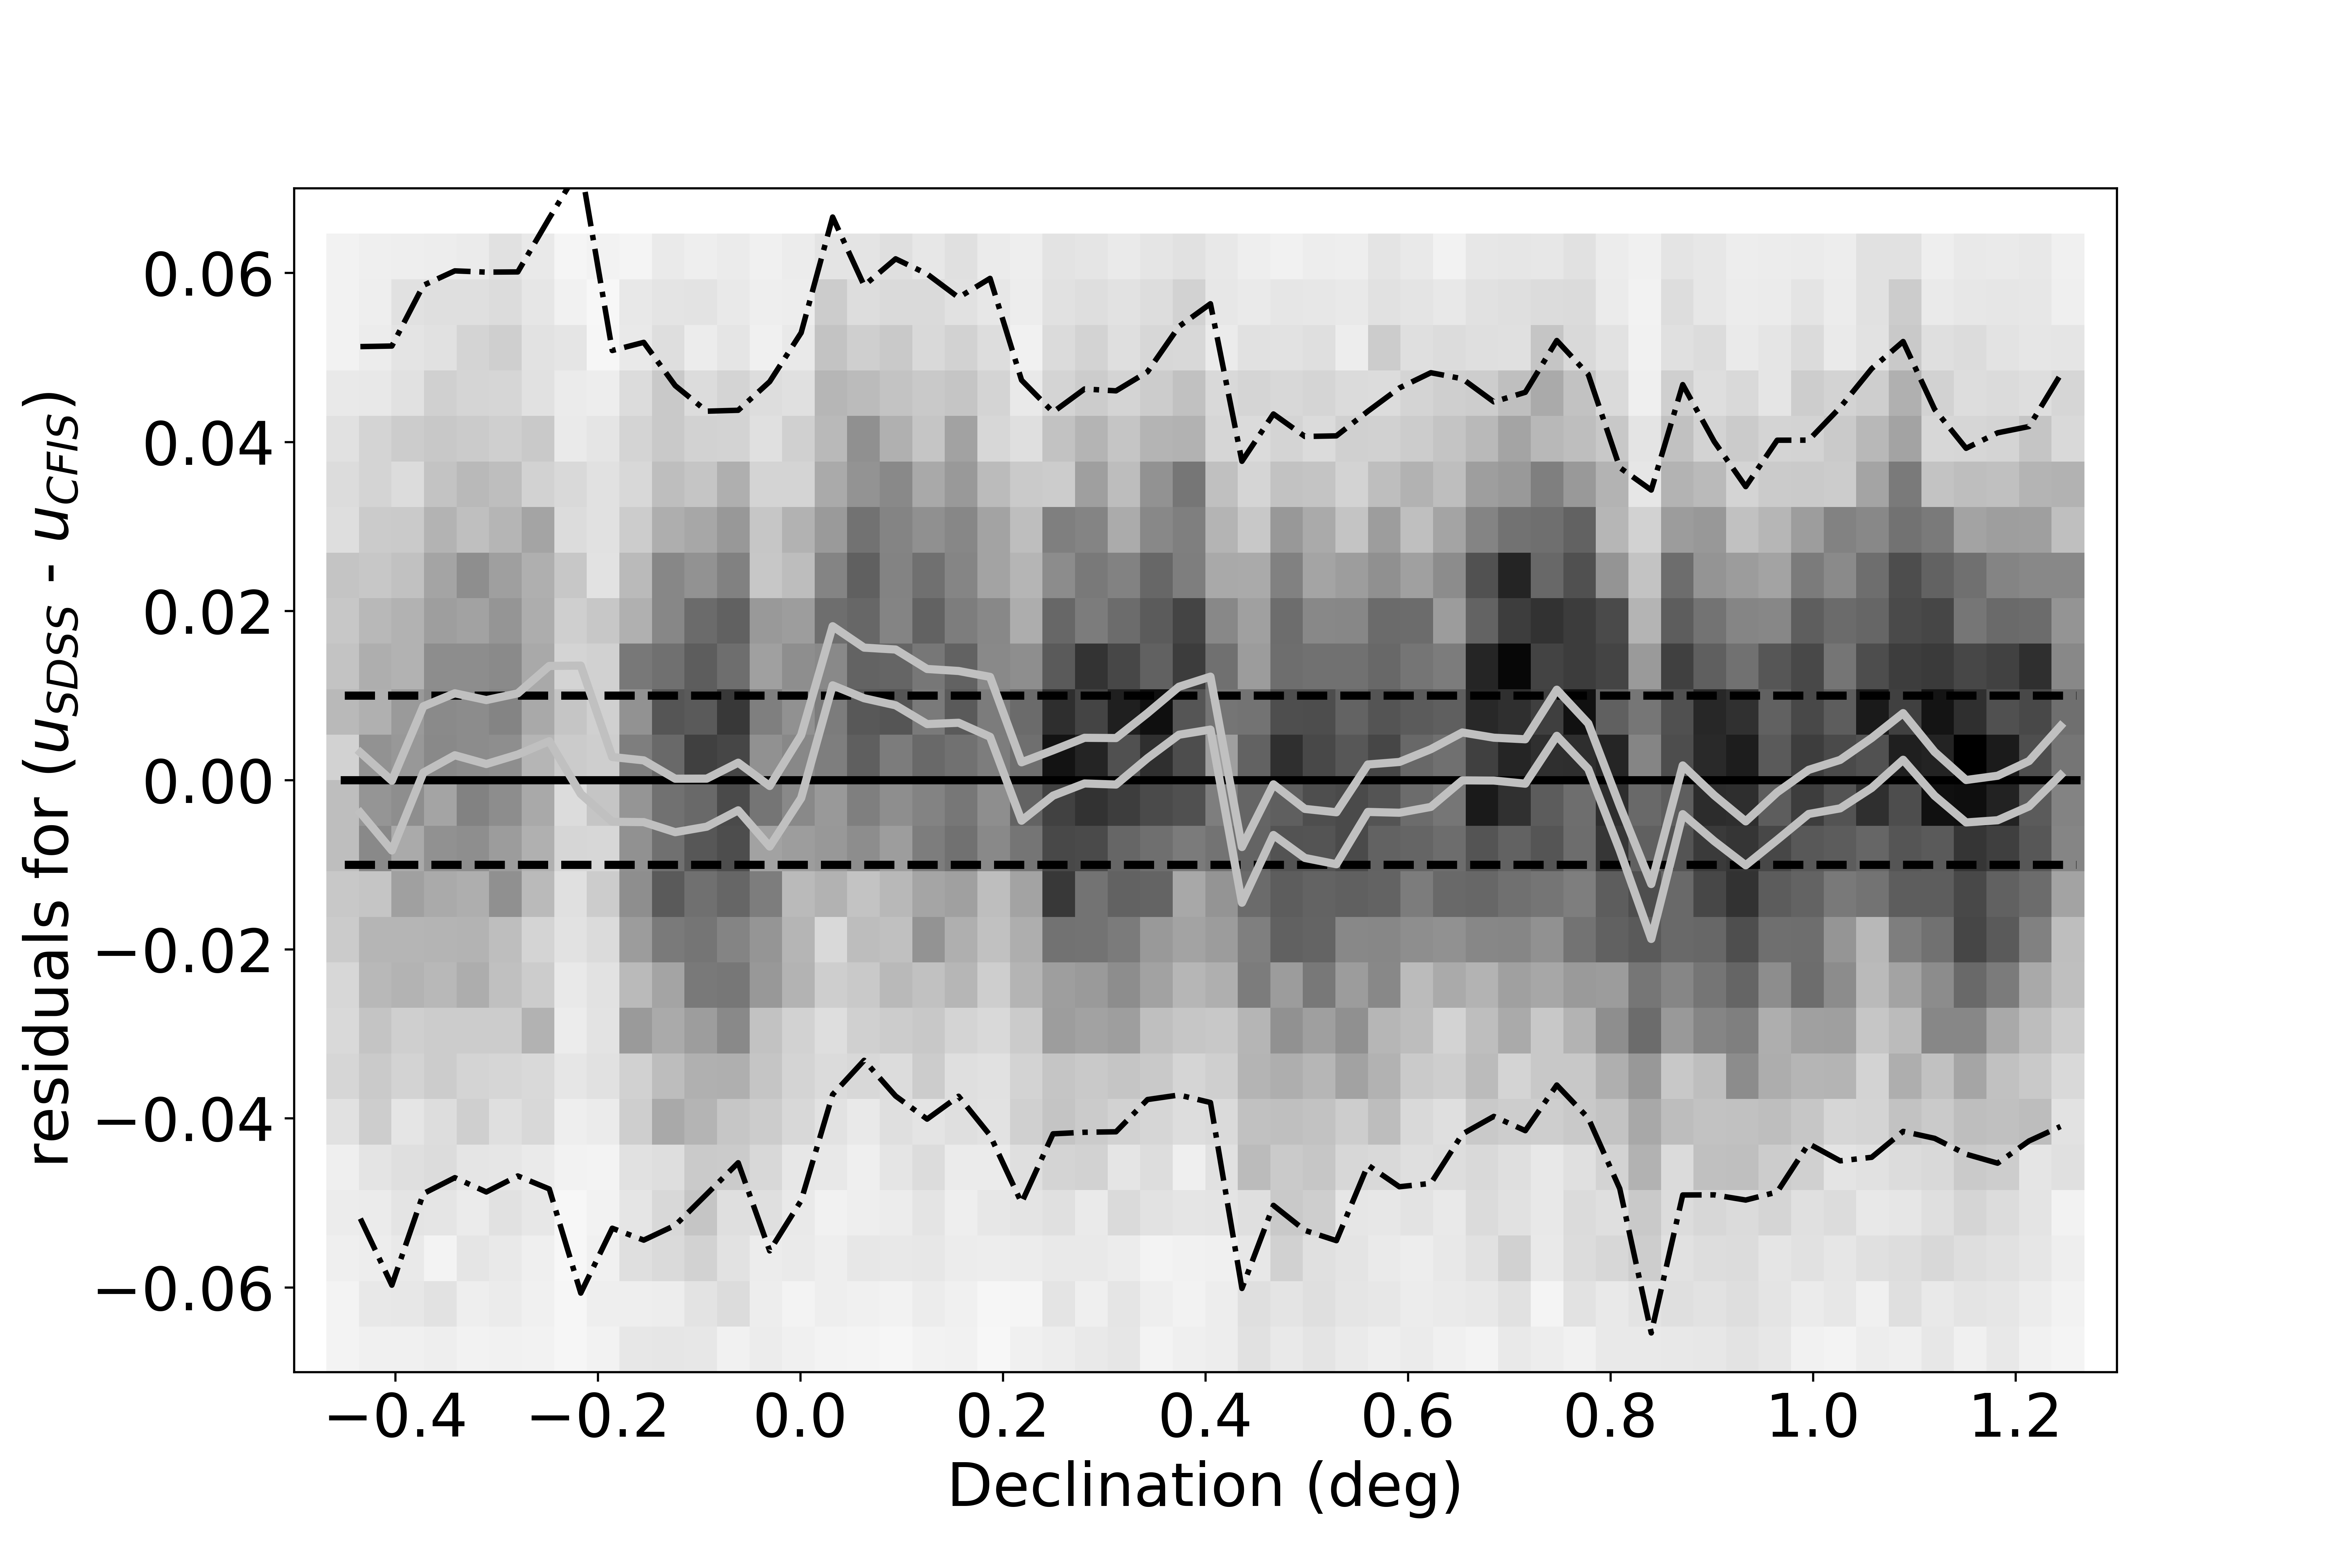
\includegraphics[width=0.95\columnwidth]{figures/colorResidCFISug_Dec_Hess.png} 
\caption{Analogous to Figure~\ref{fig:graycorrRA} ({\it Right}), except that here residuals 
between the SDSS $u$ band magnitudes and $u$ band magnitudes from the CFIS
catalog (corrected for small colour terms, $\sim0.05$ mag, as a function of the $u-g$ colour),
for $\sim$150,000 matched stars with $1.0 <u-g < 2.1$ and $r<20$ are shown. 
The binned median scatter is 5.7 millimag. Note that the CFIS data are available
only for Declination $>$ $-$0.45 degree.}
\label{fig:CFIS}
\end{figure}

%%%%%%%%%%%%%%%%%%%%%%%%%%%%%%%%%%%%%%%%%
\subsection{Comparison of the new v4.2 SDSS catalog and transformed NUV data from the GALEX catalog  \label{sec:Galextest}} 

We also use the NUV magnitudes from GALEX (see
Section~\ref{ssec:galex}) to provide an independent check on the SDSS
u-band magnitudes, following the zeropoint corrections with Gaia
photometry described in \S \ref{sec:GaiaCorr}. For this we derive the
following GALEX to SDSS u transformation equation:
%Using GALEX NUV magnitudes, with SDSS ($g$,$i$) magnitudes yields the
%tightest GALEX to SDSS u-band transformation equation. Using a second
%order fit, the fitted coefficients for the estimated SDSS $u_{est}$ is
%given by:

%\begin{equation}
%\begin{split}
%u_{est} = & NUV_{galex}  - 0.999\times(NUV_{galex} - g_{sdss}) \\
%	& + 0.015\times(NUV_{galex}  - g_{sdss})^2  \\
%         & -0.426\times(g_{sdss} - i_{sdss}) + 0.821*(g_{sdss} - i_{sdss})^2 \\
%         & + 0.939 \\
%         & + T \times [ -1.233\times(E(B-V)-0.15) + 3.430\times(E(B-V)-0.15)^{2} ] \\
%\end{split}
%\end{equation}
\begin{equation}
\begin{split}
u_{est} = & NUV - 0.990\times(NUV - g) + 0.014\times(NUV  - g)^2  \\
         & -0.407\times(g - i) + 0.797\times(g - i)^2 + 0.835  \\
         & + T \times [ -1.346\times(E(B-V)-0.15) ... \\
         & + 3.400\times(E(B-V)-0.15)^{2} ] \\
\end{split}
\end{equation}

where $NUV$ refers to GALEX, and $g$ and $i$ are SDSS magnitudes. $T$ is a step function in the value of the interstellar reddening, E(B-V),
from the \citet{1998ApJ...500..525S} reddening map:
\begin{align}
  T = \left\{ \begin{array}{cc} 
    0 & \hspace{5mm} E(B-V) \leq 0.15 \\
    1 & \hspace{5mm} 0.15 < E(B-V) < 0.3 \\
  \end{array} \right.
\end{align}
This transformation relation, which is suitable for stars with $0.5 <
(u-g)_{sdss} < 2.0$, $0.2 < (g-r)_{sdss} < 0.8$, $0.3 < (g-i)_{sdss} <
1.0$, and $E(B-V) < 0.3$, has a per star RMS of $\sigma=0.061$ mag
(the relatively high RMS is due in part to the relatively high RMS in
the GALEX $NUV$ magnitudes).  This relation converts the GALEX $NUV$
magnitudes into very reasonable approximations of the SDSS $u$-band.
To refine these approximations, we then applied the same sort of
numerical transformation that was used for the SDSS/Gaia
transformation in Figure~\ref{fig:GrVSgi}; this improved the overall
per star RMS to $\sigma=0.055$, with most of the improvement occurring
for the bluest ($(u-g)_{sdss} \la 1.0$) and the reddest ($(u-g)_{sdss}
\ga 1.0$) stars in our sample.

Despite the relatively noisy results, we can make several conclusions
based upon the binned data consisting of 89,722 matches between the
v4.2 SDSS catalog and the GALEX catalog.  First, in
Figure~\ref{fig:GALEX_umag}, we show the difference between the
SDSS-measured and GALEX-predicted $u_{sdss}$ vs. SDSS $u_{sdss}$ for
the 80,053 matches that lie within the colour and $E(B-V)$ cuts used
for the initial transformation equation (Eq.~1).  Although the
relation, even when binned like here, is noisy, there is clearly a
noticeable trend in the residuals vs. SDSS $u$.  As with the
comparison with Gaia (Fig~\ref{fig:gaiaJump}, we expect that this
magnitude dependence is associated with the GALEX photometry rather
than with SDSS.  Second, in Figure~\ref{fig:GALEX_RA} ({\it Left}), we plot this
magnitude difference vs. RA along SDSS Stripe 82.  Here, in addition
to the cuts used for Figure~\ref{fig:GALEX_umag}, we also apply a cut
of $u_{sdss}\le20.0$, to avoid the worst deviations seen in that
figure; this results in a sample of 69,783 matches.  We do note some
small but significant large-scale trends with RA, at the 9.5 millimag
level (RMS).  
%Here, a noticeable large-scale trends can
%indeed be seen at the $\sim$0.01-0.02 mag level.  It is interesting
%that these trends in $u$ are qualitatively similar -- but opposite in
%sign -- to some of the trends seen in the comparison plots with DES
%and Pan-STARRS1 in Section~\ref{sec:DESPS1} (see, e.g.,
%Fig.~\ref{fig:DESPSRA}). {\bf (DLT: Check this!)}.
Third and finally, in Figure~\ref{fig:GALEX_RA} ({\it Right}), we plot this
magnitude difference vs. DEC across SDSS Stripe82 using the same
sample of 69,783 matches used for Figure~\ref{fig:GALEX_RA} ({\it Left}).  Unlike
for the CFIS comparison in the previous section (see, e.g.,
Fig.~\ref{fig:CFIS}, the GALEX comparison covers the full DEC range of
Stripe 82.  Overall, aside of a possible slight gradient, there appear
to be no strong large-scale trends.  The hints of smaller scale
($\sim0.4^{\circ}$) variations -- roughly on the scale of a SDSS
camera column -- seen in the CFIS comparison (Fig.~\ref{fig:CFIS}),
however, are not seen here, perhaps due to the relative ``noisiness''
of the GALEX comparison.


\begin{figure}
    \centering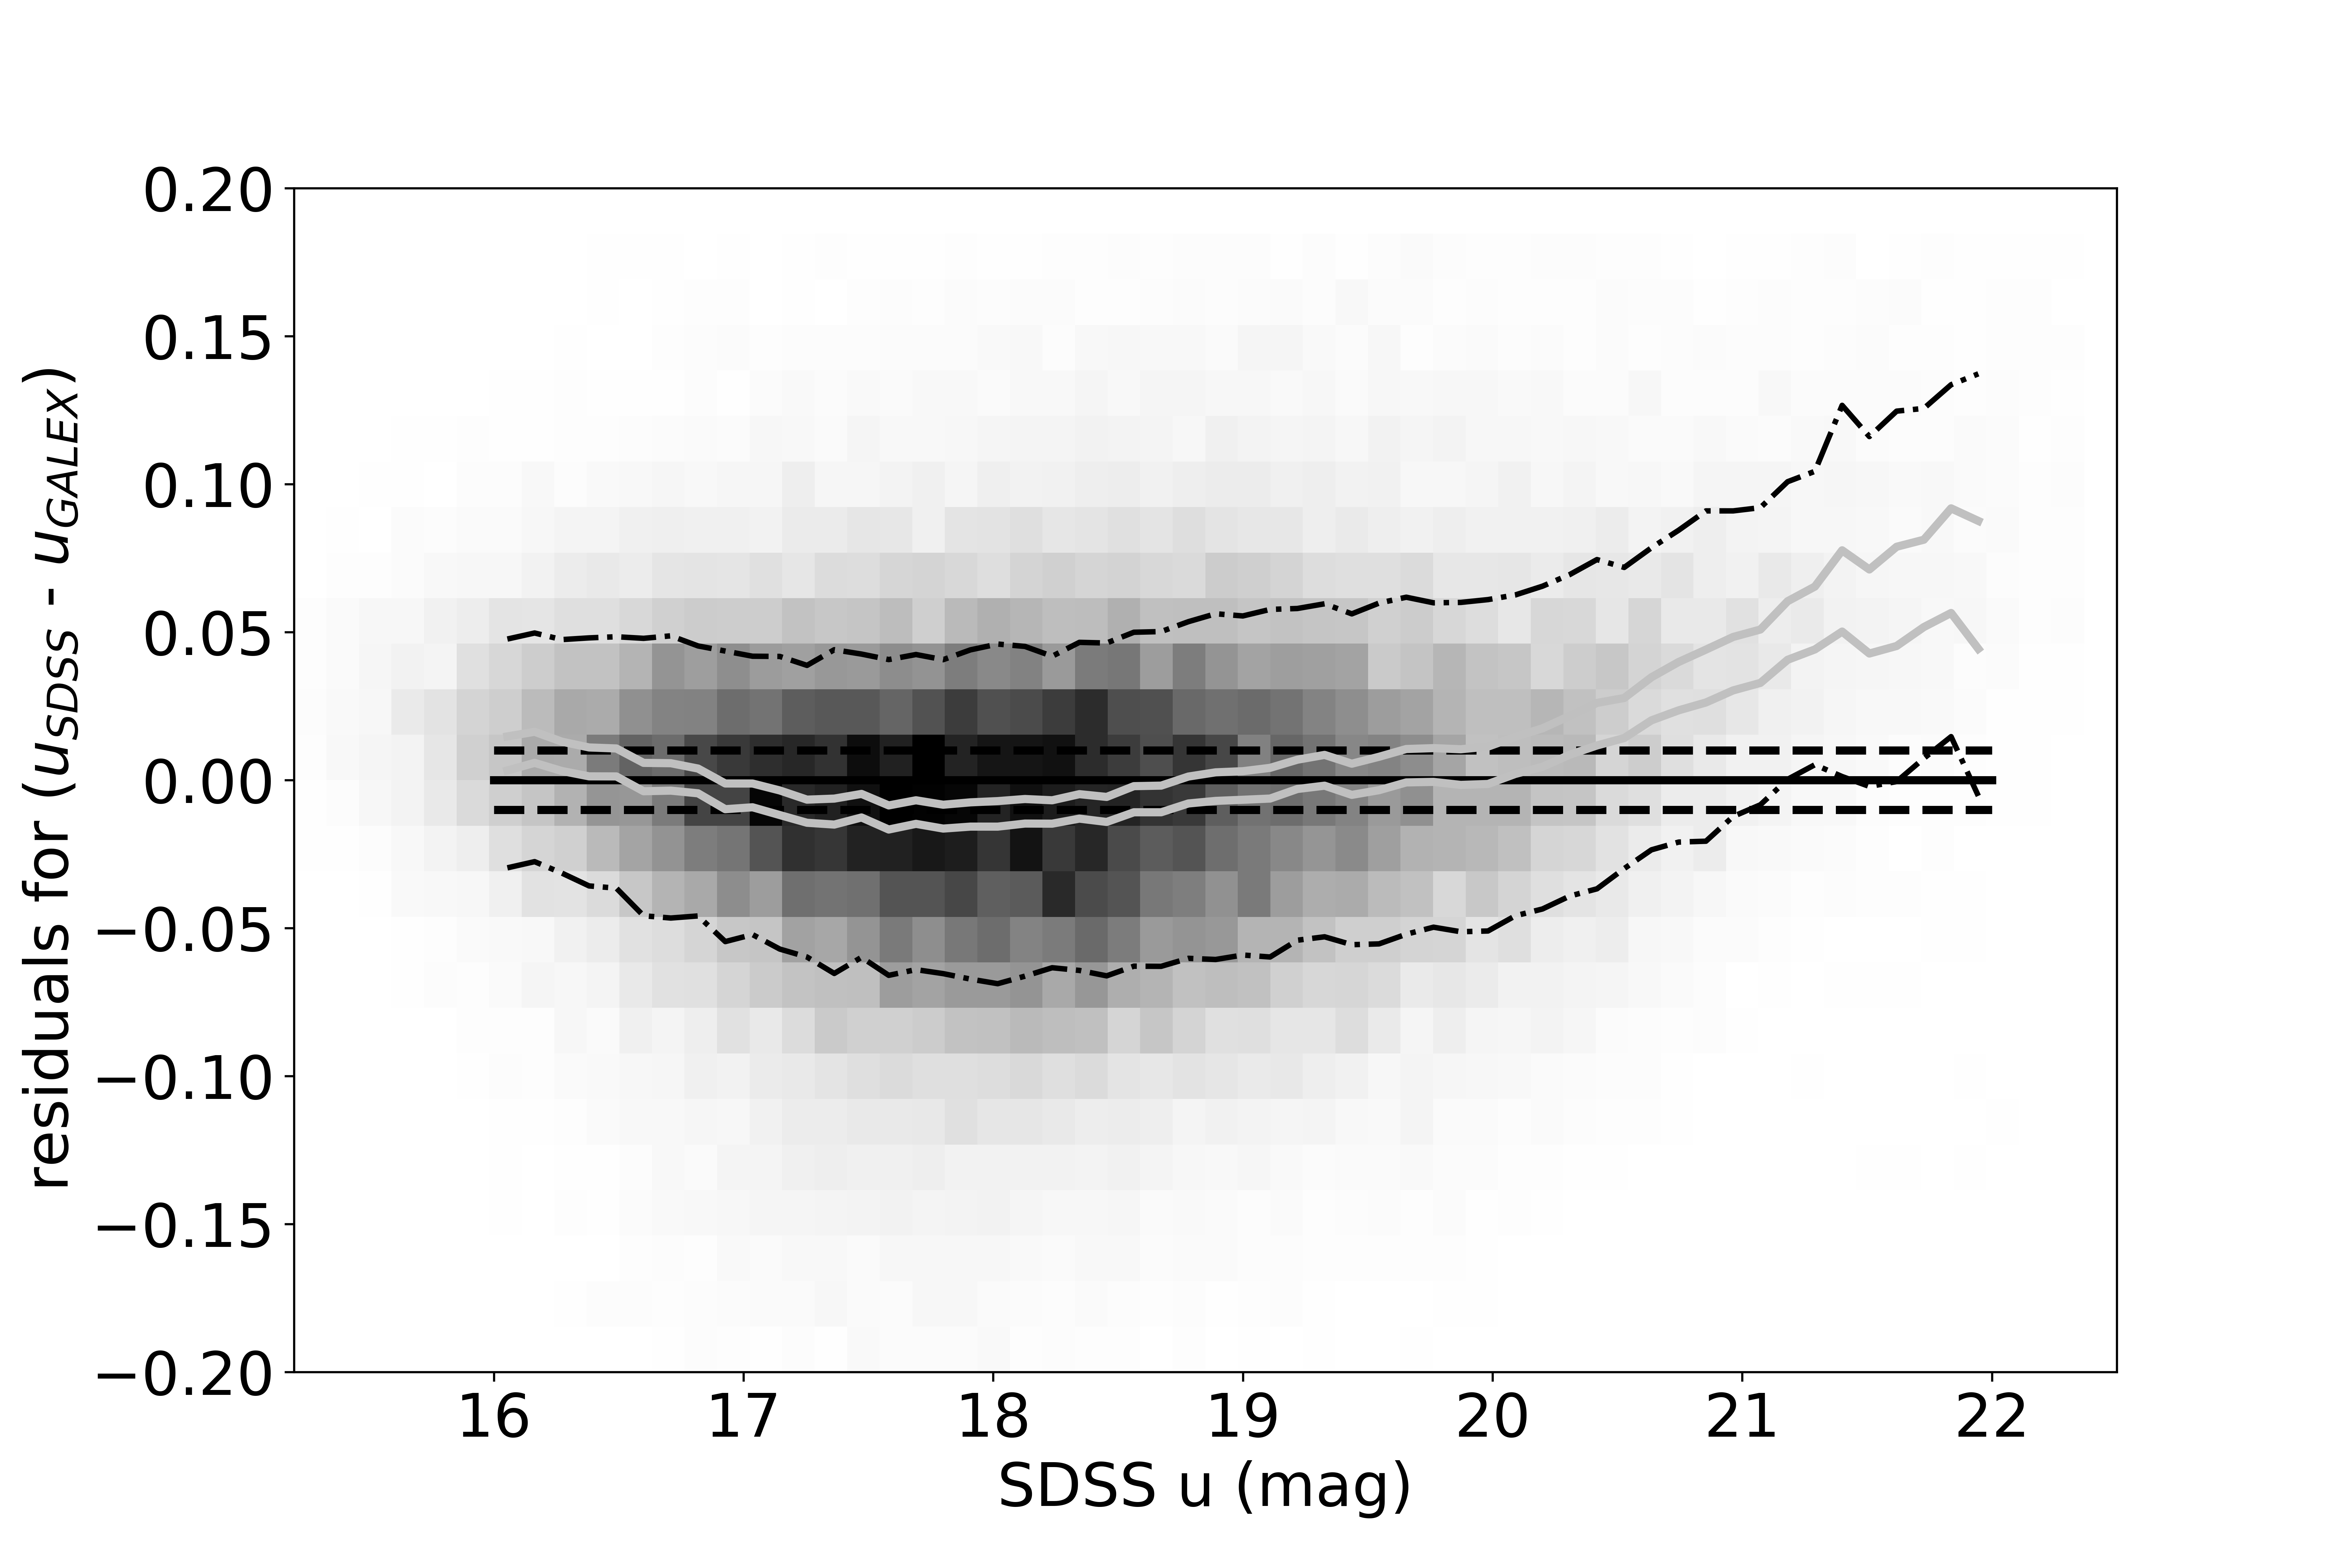
\includegraphics[width=0.95\columnwidth]{figures/colorResidGALEXug_du_est_umag_Hess.png}
\caption{Analogous to Figure~\ref{fig:gaiaJump}, except that here
  residuals residuals between the SDSS $u$ band magnitudes and
  predicted $u$ band magnitudes transformed from the GALEX catalog are
  shown.  The individual star scatter is 54.5 millimag (dot-dashed
  lines); the binned median scatter is 24.5 millimag solid grey
  lines).
}
\label{fig:GALEX_umag}
\end{figure}



\begin{figure*}
    \centering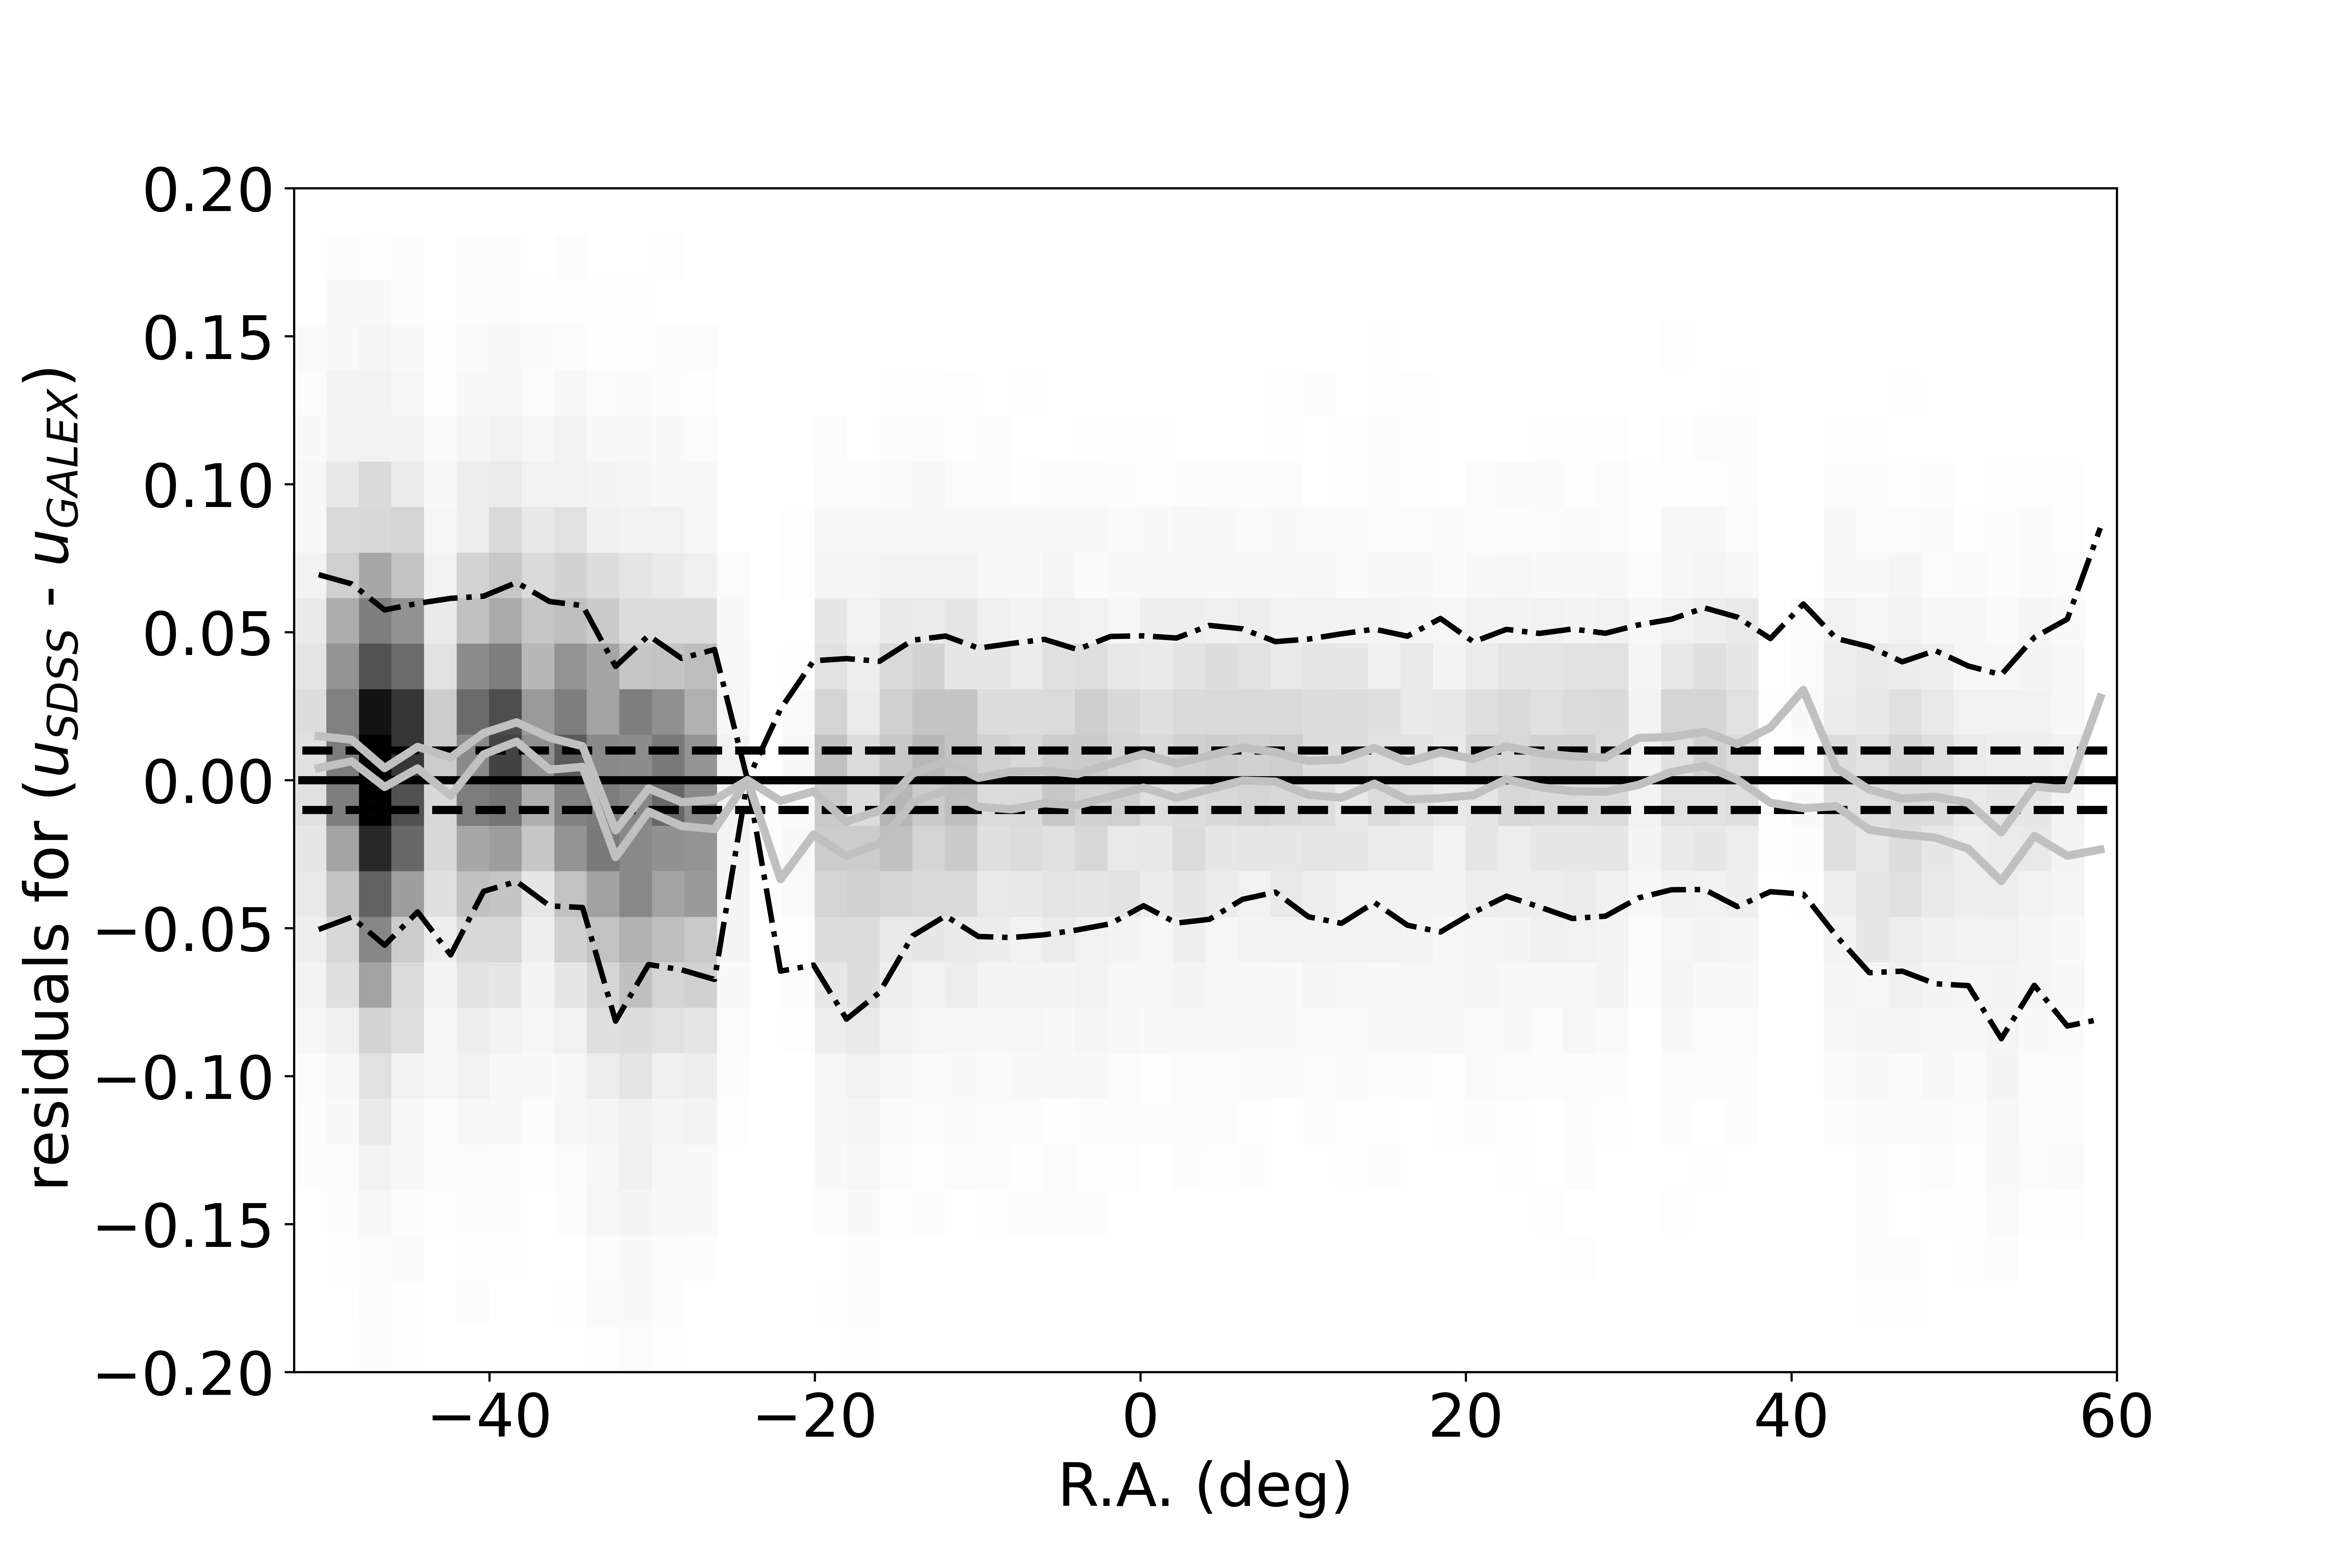
\includegraphics[width=0.95\columnwidth]{figures/colorResidGALEXbright_du_est_RA_Hess.png}
    \centering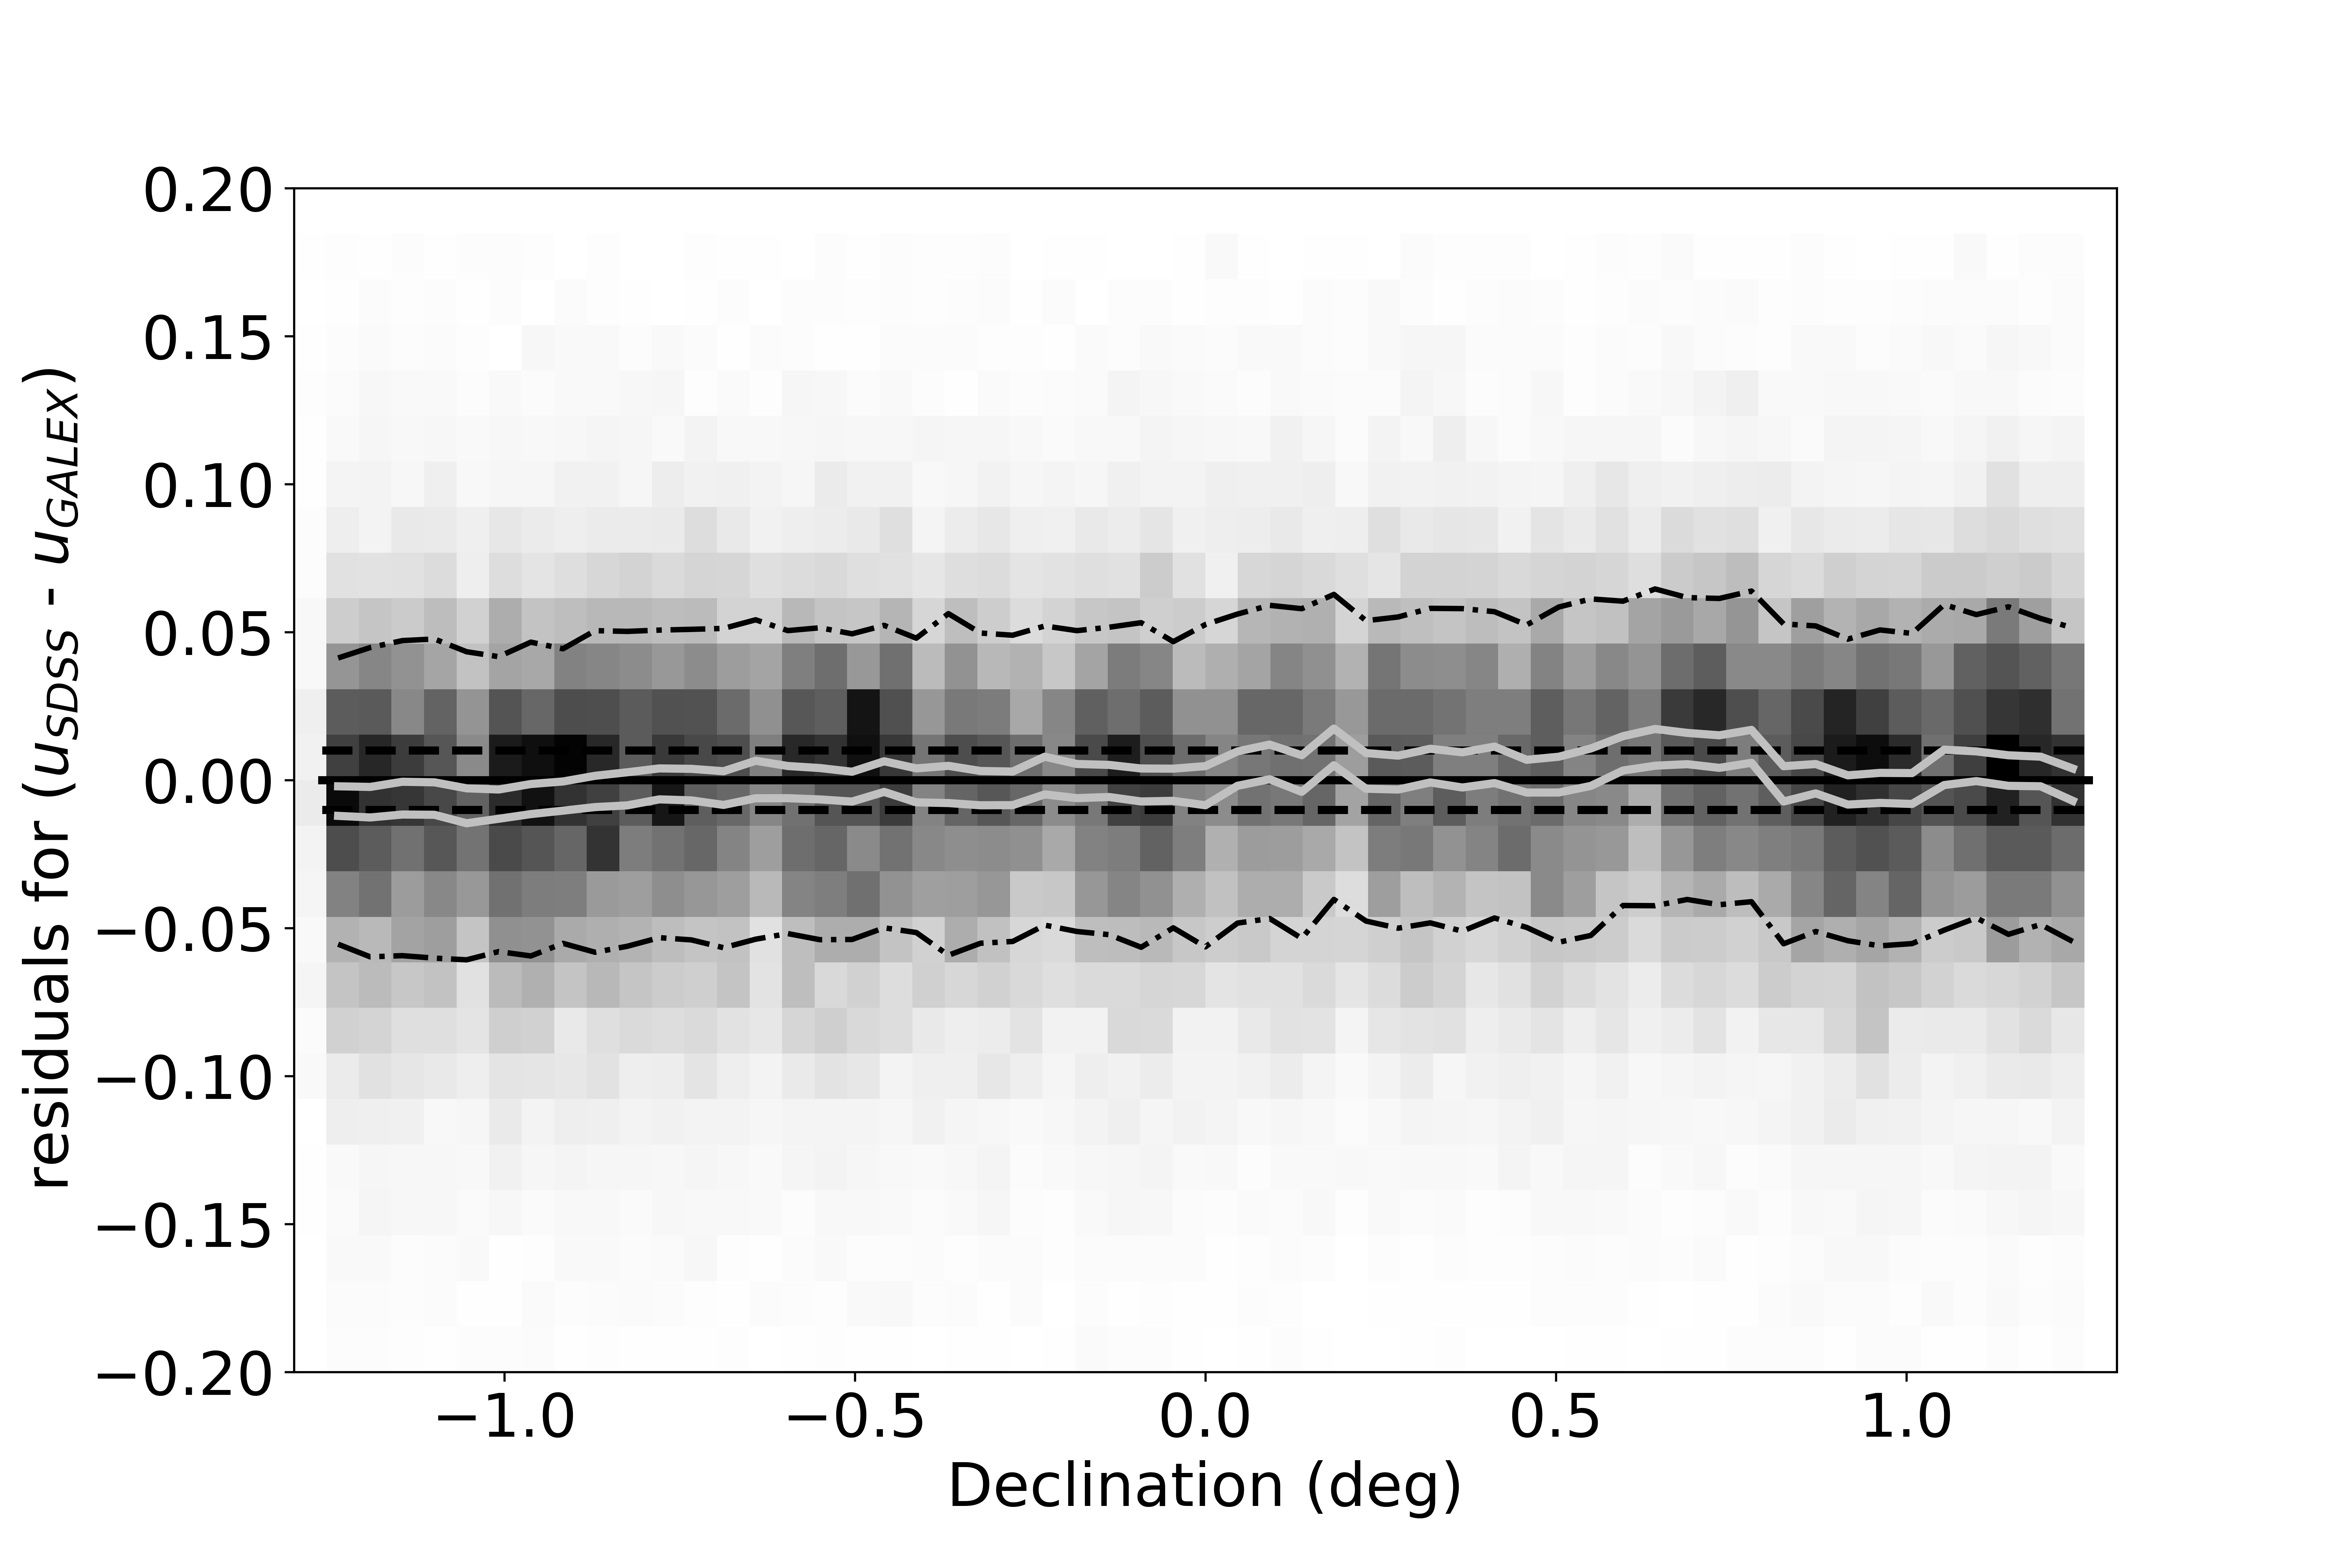
\includegraphics[width=0.95\columnwidth]{figures/colorResidGALEXbright_du_est_Dec_Hess.png}
\caption{({\it Left}) Analogous to Figure~\ref{fig:graycorrRA} ({\it Left}), except that here
  residuals between the SDSS $u$ band magnitudes and
  predicted $u$ band magnitudes transformed from the GALEX catalog are
  shown.  Unlike in Figure~\ref{fig:GALEX_umag}, we exclude matches for
  which SDSS $u$$>$20.0 The individual star scatter is 52.9 millimag
  (dot-dashed lines); the binned median scatter is 9.5 millimag (solid
  grey lines). ({\it Right}) Analogous to Figure~\ref{fig:graycorrRA} ({\it Right}), except that here
  residuals residuals between the SDSS $u$ band magnitudes and
  predicted $u$ band magnitudes transformed from the GALEX catalog are
  shown.  Unlike in Figure~\ref{fig:GALEX_umag}, we exclude matches
  for which SDSS $u$$>$20.0 The individual star scatter is 52.9
  millimag (dot-dashed lines); the binned median scatter is 5.0
  millimag (solid grey lines). 
}
\label{fig:GALEX_RA}
\end{figure*}



% \begin{figure}
%    \centering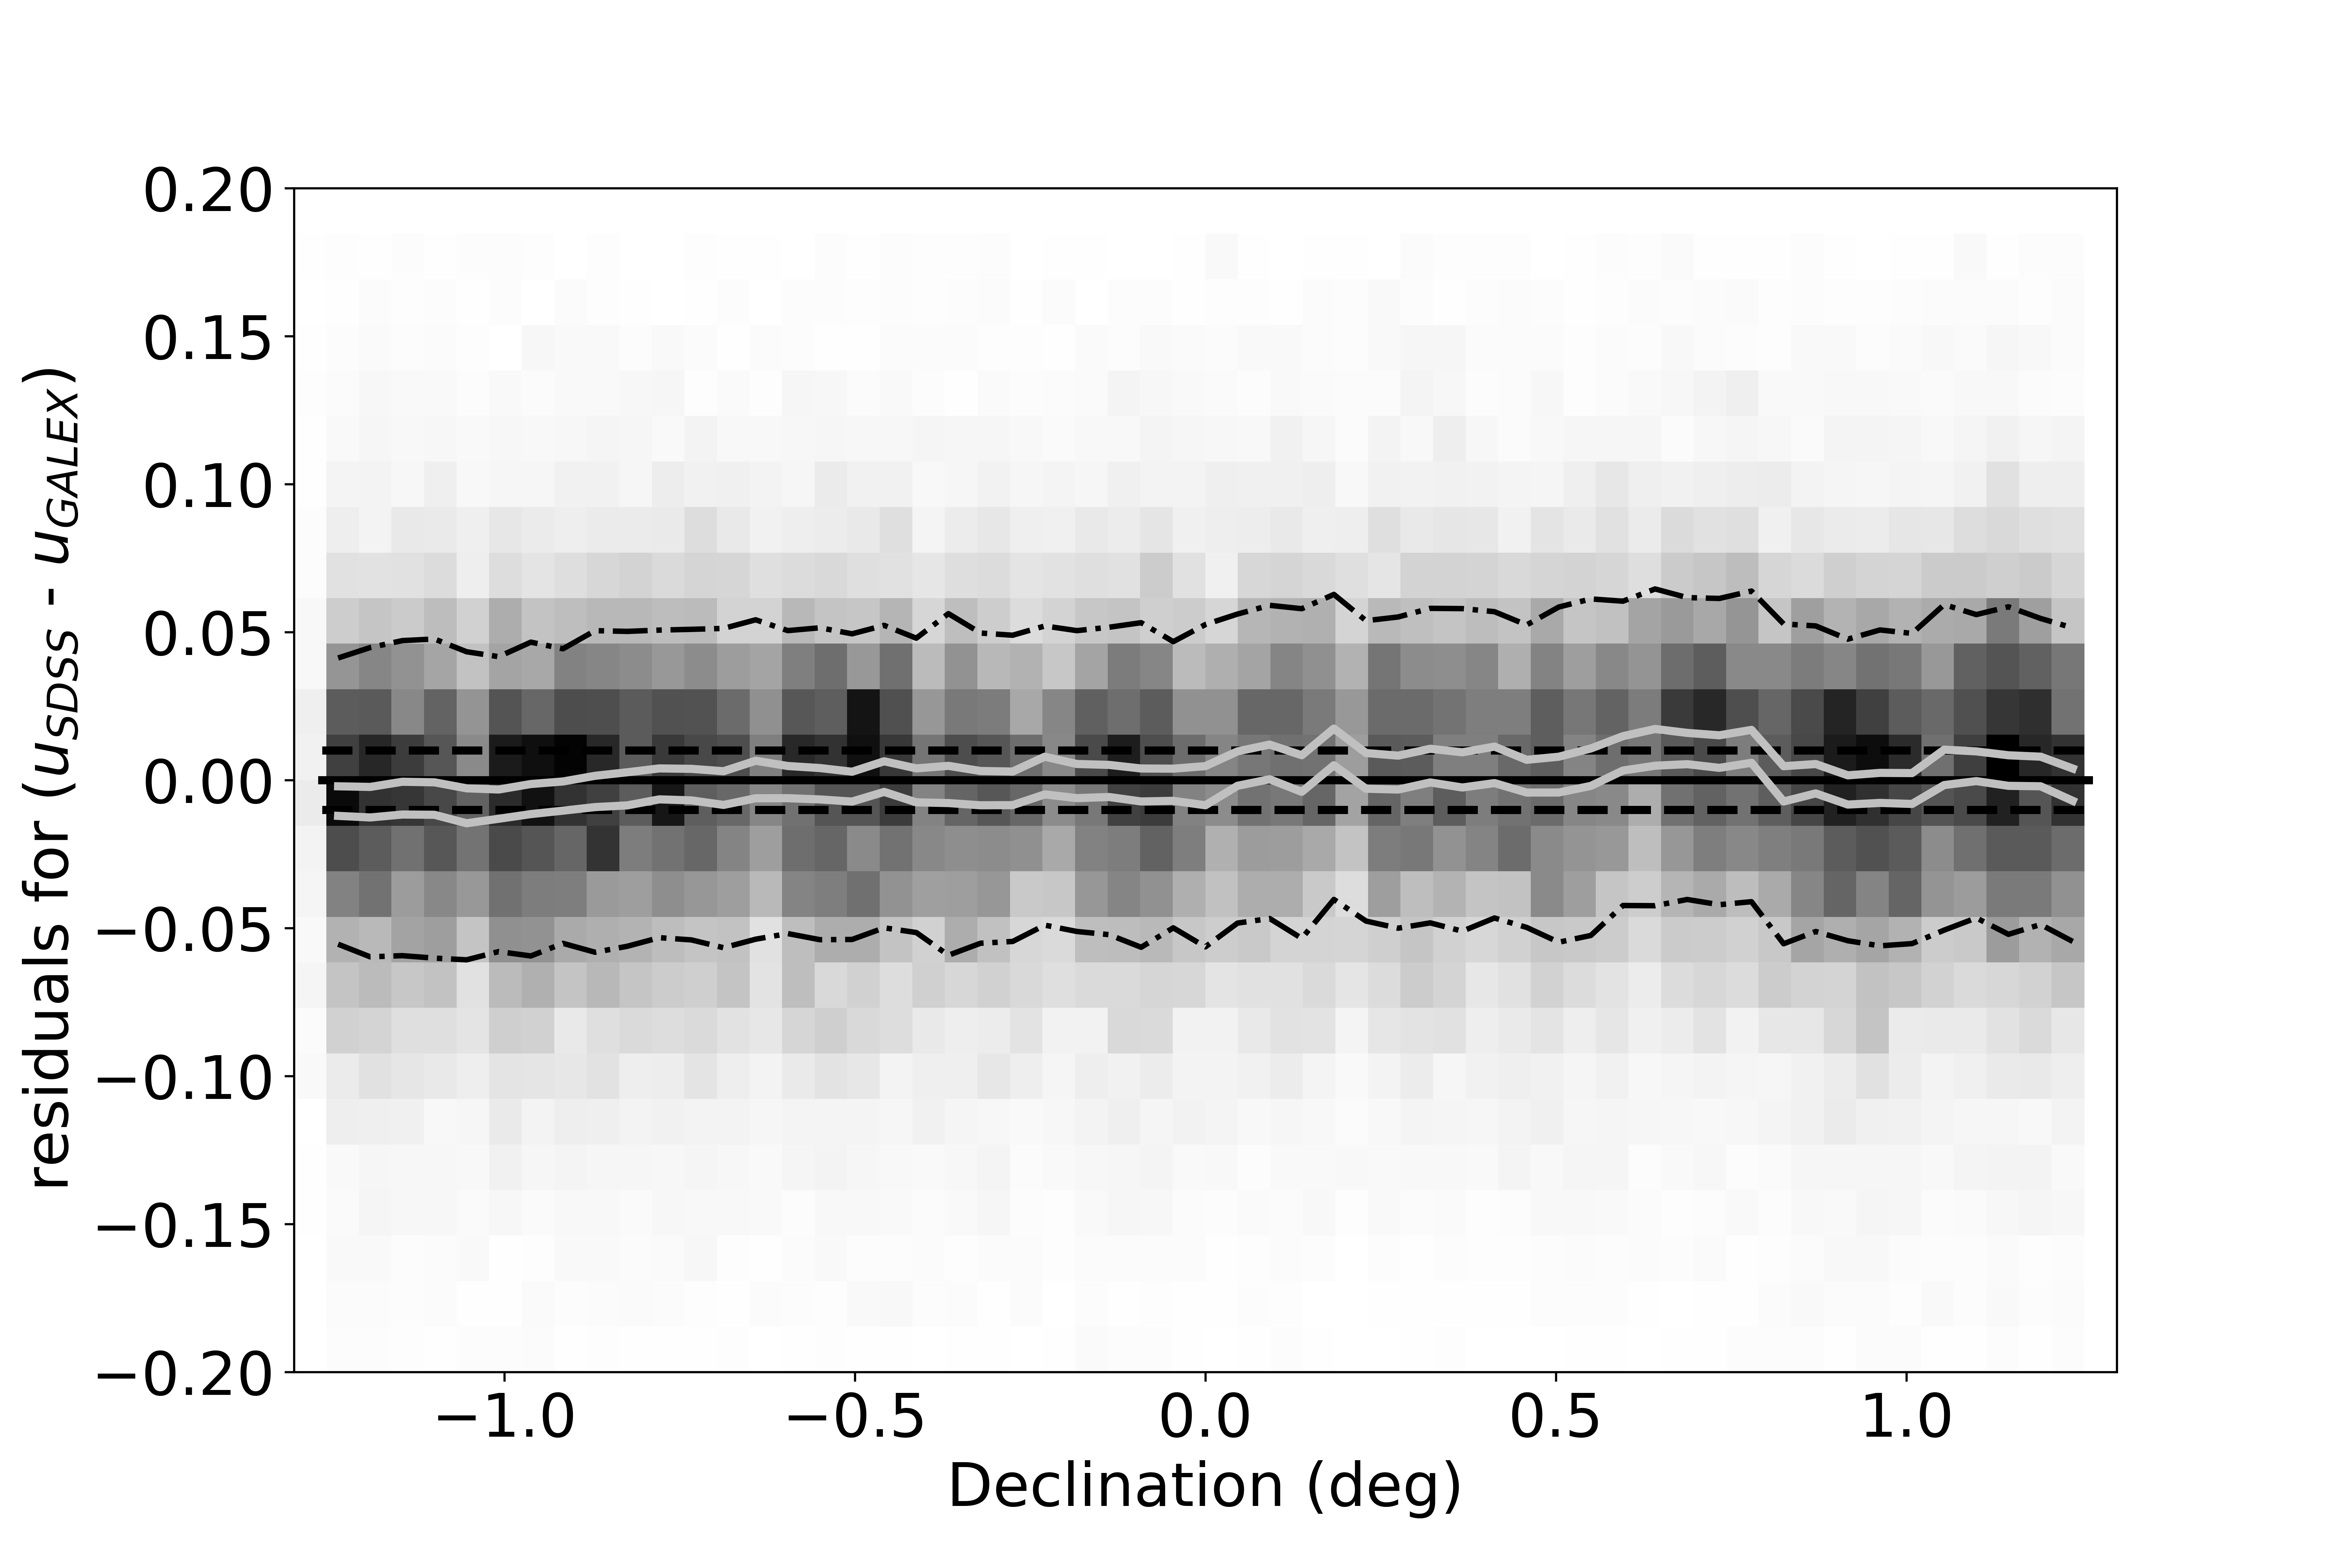
\includegraphics[width=0.95\columnwidth]{figures/colorResidGALEXbright_du_est_Dec_Hess.png}
%\caption{Analogous to Figure~\ref{fig:graycorrRA} ({\it Right}), except that here
%  residuals residuals between the SDSS $u$ band magnitudes and
%  predicted $u$ band magnitudes transformed from the GALEX catalog are
%  shown.  Unlike in Figure~\ref{fig:GALEX_umag}, we exclude matches
%  for which SDSS $u$$>$20.0 The individual star scatter is 52.9
 % millimag (dot-dashed lines); the binned median scatter is 5.0
%  millimag (solid grey lines).  }
%\label{fig:GALEX_Dec}
%\end{figure}

%%%%%%%%%%%%%%%%%%%%%%%%%%%%%%%%%%%%%%%%%

\subsection{Offsets from AB magnitude scale \label{sec:AB}} 

We estimate offsets from the AB magnitude scale using synthetic photometry derived from the spectra of three DA white dwarfs observed by HST (see Table~\ref{tab:HST}): GD50 (specifically, the calibrated spectrum file {\tt gd50\_004.fits}) from the HST CalSpec database of spectrophotometric standard stars \citep{2014PASP..126..711B}\footnote{https://www.stsci.edu/hst/instrumentation/reference-data-for-calibration-and-tools/astronomical-catalogs/calspec}, and SDSSJ~232941.32$+$001107.8 and SDSSJ~010322.19-002047.7 from \citet{2019ApJS..241...20N}
(the flux-calibrated modeled spectrum files provided by G. Narayan, private communication).  These three spectrophotometric calibrators are particularly useful for our purposes since they are faint enough not to be saturated in the SDSS photometry ($r>14$) and they lie within the SDSS Stripe 82 footprint, making direct comparison to the SDSS measurements relatively simple.  Synthetic AB magnitudes for these three DA white dwarfs were derived via numerical integration of Equation~8 of \citet{1996AJ....111.1748F}, which serves to define broad-band AB magnitudes.  This equation requires not only a well-calibrated spectrum, but also the well-calibrated bandpass response curves for the photometric system in question.  Here, we make use of the SDSS bandpass response curves from Table~4 of \citet{2010AJ....139.1628D}.  Our results for the synthetic SDSS AB magnitues for these three stars can be found in Table~\ref{tab:HST}.  The errors on these synthetic AB magnitudes are expected to be $\sim$5--10~millimag (statistical) and $\sim$10~millimag (systematic) (e.g., \citet{2014PASP..126..711B}).  




%XXX Doug expands this section, refers to G. Narayan et al. (2019) and other refs,
%and other details explaining how synthetic ugriz photometry is generated for these three stars...

% From Doug's email: 
% As to the precision and accuracy of the synthetic mags, that is a little hard to quantify.  Narayan et al (2019) report 
% uncertainties for the synthetic magnitudes of the 2 DA?s from their sample at about 0.5% (5 milli-mags), but I don?t know if 
% that includes uncertainties in the reddening and in version of the SDSS filters used.  The HST CalSpec database (which 
% included GD50) is usually quoted as having an accuracy of about 1% (10 milli-mags) in the optical on average for any given 
% star in its database. 
% When I get observed DA WD spectra modeled by Pier-Emmanuel Tremblay (a former postdoc of Bergeron), he sends me not 
% only the best-fit model but also the +/-1sigma Teff, logg models as well.  When I calculate the synthetic mags for those, I
% usually get a spread of less than 1% in the resulting synthetic mags; so I think Gautham Narayan?s estimate of a statistical
% RMS of 0.5% for his models is reasonable.  So maybe 0.5% (5 millimag) precision/statistical error, and c. 1% (10 milli-mags)
% accuracy/systematic error.

Table~\ref{tab:AB} presents the numerical summary of the comparison between SDSS magnitudes 
and HST-based synthetic magnitudes for three white dwarfs. We used unweighted mean because 
formal uncertainties for SDSS photometry are subdominant to systematic errors in HST-based
synthetic magnitudes, estimated at about 0.01 mag. Uncertainty of the mean offsets was 
computed from the observed scatter of three values. In the $riz$ bands we detect significant
($>3\sigma$) deviations, ranging from 0.012 mag to 0.033 mag, while in the $u$ and $g$ bands 
we can only place upper limits (at $2\sigma$: 0.038 mag and 0.028 mag, respectively). 

% \begin{deluxetable}{r|r|r|l|l|l|l|l}[ht!]
% \tablecaption{Synthetic SDSS magnitudes for three WD dwarfs with HST photometry$^a$. \label{tab:HST}}
% \tablehead{
%   \colhead{Name} & \colhead{R.A. } & \colhead{Dec.} & \colhead{u} & \colhead{g} & \colhead{r} & \colhead{i} & \colhead{z} 
% }
% \startdata
%      GD50                     &  57.2091083 &  $-$0.975636 &      13.409 &       13.784 &    14.295 &     14.655 &     \nodata$^b$ \\
%      SDSSJ~232941.32+001107.8 & 352.4221875 &     0.185500 &      18.154 &       18.145 &    18.466 &     18.754 &     19.042 \\  
%      SDSSJ~010322.19-002047.7 &  15.8424625 &  $-$0.346592 &      18.627 &       19.057 &    19.558 &     19.923 &     20.258 \\
%     GD50                     &  57.2091083 &  $-$0.975636 &      13.409 &       13.784 &    14.295 &     14.655 &     99.999$^b$ \\
% \enddata
% \tablenotetext{a}{Give here reference to HST data, or some other comment?} 
% \tablenotetext{b}{The CalSpec spectrum stopped at about 9000 \AA and thus did not cover all of SDSS $z$ band.} 
% \end{deluxetable}

\begin{table*}
	\centering
	\caption{Synthetic SDSS magnitudes for three WD dwarfs with HST photometry$^a$.}
	\label{tab:HST}
	\begin{tabular}{r|r|r|l|l|l|l|l} % 
		\hline
		Name & R.A. & Dec. & u & g & r & i & z \\
		\hline
     GD50                     &  57.2091083 &  $-$0.975636 &      13.409 &       13.784 &    14.295 &     14.655 &     {\it no data}$^b$ \\
     SDSSJ~232941.32+001107.8 & 352.4221875 &     0.185500 &      18.154 &       18.145 &    18.466 &     18.754 &     19.042 \\  
     SDSSJ~010322.19-002047.7 &  15.8424625 &  $-$0.346592 &      18.627 &       19.057 &    19.558 &     19.923 &     20.258 \\
		\hline
	\end{tabular}
     \vspace{1ex}

     {\raggedright {\bf Notes}: (a) \tbd{Give here reference to HST data, or some other comment?} \newline (b) The CalSpec spectrum stopped at about 9000 \AA and thus did not cover all of SDSS $z$ band.\par}
\end{table*}


% \begin{deluxetable}{l|r|r|r|r|r}[ht!]
% \\tablecaption{AB offsets implied by three WD dwarfs with HST photometry$^a$. \label{tab:AB}}
% \\tablehead{
% \      & \colhead{$\Delta u$}  & \colhead{$\Delta g$}  & \colhead{$\Delta r$}  & \colhead{$\Delta i$}  & \colhead{$\Delta z$}  
% \}
% \\startdata 
% \   {\rm mean}            &    $-$0.009    &        0.000     &      0.015    &       0.016    &      0.035     \\ 
% \  $\sigma_{\rm mean}$ &         0.019    &        0.014     &      0.004    &       0.004    &      0.011     \\
% \\enddata
% \\tablenotetext{a}{Offsets are defined as additive corrections to SDSS photometry to place it on AB scale (in mag). 
% \Listed values are unweighted mean and its uncertainty.}  
% \\end{deluxetable}

\begin{table}
	\centering
	\caption{AB offsets implied by three WD dwarfs with HST synthetic photometry$^a$.}
	\label{tab:AB}
	\begin{tabular}{l|r|r|r|r|r} % 
		\hline
		& $\Delta u$ & $\Delta g$ &$\Delta r$ &$\Delta i$ &$\Delta z$ \\
		\hline
  		 {\rm mean}            &    --     &        --     &      0.015    &       0.016    &      0.035     \\ 
  		$\sigma_{\rm mean}$ &         0.019    &        0.014     &      0.004    &       0.004    &      0.011     \\
		\hline
	\end{tabular}
     \vspace{1ex}

     {\raggedright {\bf Notes}: (a) Offsets are defined as additive corrections to SDSS photometry to place it on AB scale (in mag). Listed values are unweighted mean and its uncertainty. \par}
\end{table}
% $-$0.009  0.000


%%%%%%%%%%%%%%%%%%%%%%%%%%%%%%%%%%%%%%%%%%%%%%%%%%
\section{Discussion and Conclusions} \label{sec:disc}

To enable further progress in cosmological and other high-precision photometric measurements, 
modern multi-band photometric sky surveys aim to deliver measurements accurate at the 1\% 
(0.01 mag) level. Over the last decade a number of such large-scale surveys approached, and
often exceeded this photometric accuracy threshold. For ground-based surveys, which are 
affected by variable atmospheric effects and hardware responses to changes in local environment
(e.g. temperature), significant improvements are achieved by averaging multiple observations. 

In this paper, we have described the construction and tests of an updated version of the
SDSS Stripe 82 Standard Star catalog \citep{Ivez07} that lists averaged SDSS photometry for about
a million non-variable stars. Additional post-2007 SDSS data include about 
2-3 times more measurements per star than in the original catalog, resulting in 1.4-1.7 times smaller 
random photometric errors (precision) than in the original catalog, and about three times as small 
as for individual SDSS runs.

Thanks to the availability of photometric data from recent wide-field surveys (Gaia, DES, Pan-STARRS
and CFIS), we were able to derive robust zeropoint corrections and establish that this new catalog
is superior to the original catalog. Using a combination of comparison to other catalogs and 
astrophysical constraints, we find that that the contribution of the zeropoint errors to photometric
uncertainties is $<5$ millimag for the $gri$ bands, and $<10$ millimag for the $u$ and $z$ bands. 

Various catalog cross-comparisons have revealed minor problems with all the analyzed catalogs.
For example, we detected DES $z$ band zeropoint errors of up to 0.01-0.02 mag, as a function 
of R.A., and demonstrated that Gaia Gmag magnitudes appear too faint by about 0.02 mag at
Gmag$\sim$20.
 
We constrained offsets from the absolute AB magnitude scale using three white dwarfs with the 
HST CalSpec absolute photometry data. In the $riz$ bands we measured significant ($>3\sigma$) 
deviations, ranging from 0.015 mag to 0.035 mag (see Table~\ref{tab:AB}), while in the $u$ and $g$ 
bands we only placed upper limits (at $2\sigma$: 0.038 mag and 0.028 mag, respectively). These
constraints on absolute AB magnitude scale could be improved by extend the number of such 
calibrators.

Thanks to its high stellar density, about 1 star per square arcmin, and demonstrated sub-percent 
internal photometric precision, this catalog is a good resource for both calibrating and testing 
other surveys. In particular, it will enable high-precision photometric testing of data collected 
during the commissioning phase of the Rubin Observatory Legacy Survey of Space and Time. 

%%%%%%%%%%%%%%%%%%%%%%%%%%%%%%%%%%%%%%%%%%%%%%%%%%
\newpage

\section*{Acknowledgements}

{\bf SDSS-IV, DR15} Funding for the Sloan Digital Sky Survey IV has been provided by the Alfred P. Sloan Foundation, the U.S. Department of Energy Office of Science, and the Participating Institutions. SDSS acknowledges support and resources from the Center for High-Performance Computing at the University of Utah. SDSS is managed by the Astrophysical Research Consortium for the Participating Institutions of the SDSS Collaboration including the Brazilian Participation Group, the Carnegie Institution for Science, Carnegie Mellon University, Center for Astrophysics at Harvard \& Smithsonian (CfA), the Chilean Participation Group, the French Participation Group, Instituto de Astrof{\'i}sica de Canarias, The Johns Hopkins University, Kavli Institute for the Physics and Mathematics of the Universe (IPMU) / University of Tokyo, the Korean Participation Group, Lawrence Berkeley National Laboratory, Leibniz Institut f{\"u}r Astrophysik Potsdam (AIP), Max-Planck-Institut f{\"u}r Astronomie (MPIA Heidelberg), Max-Planck-Institut f{\"u}r Astrophysik (MPA Garching), Max-Planck-Institut f{\"u}r Extraterrestrische Physik (MPE), National Astronomical Observatories of China, New Mexico State University, New York University, University of Notre Dame, Observat{\'o}rio Nacional / MCTI, The Ohio State University, Pennsylvania State University, Shanghai Astronomical Observatory, United Kingdom Participation Group, Universidad Nacional Aut?noma de M{\'e}xico, University of Arizona, University of Colorado Boulder, University of Oxford, University of Portsmouth, University of Utah, University of Virginia, University of Washington, University of Wisconsin, Vanderbilt University, and Yale University. \\
{\bf Gaia EDR3}: This work has made use of data from the European Space Agency (ESA) mission {\it Gaia} (\url{https://www.cosmos.esa.int/gaia}), processed by the {\it Gaia} Data Processing and Analysis Consortium (DPAC,\url{https://www.cosmos.esa.int/web/gaia/dpac/consortium}). Funding for the DPAChas been provided by national institutions, in particular the institutions participating in the {\it Gaia} Multilateral Agreement.\\
{\bf DES DR1}: This project used public archival data from the Dark Energy Survey (DES). Funding for the DES Projects has been provided by the U.S. Department of Energy, the U.S. National Science Foundation, the Ministry of Science and Education of Spain, the Science and Technology FacilitiesCouncil of the United Kingdom, the Higher Education Funding Council for England, the National Center for Supercomputing Applications at the University of Illinois at Urbana-Champaign, the Kavli Institute of Cosmological Physics at the University of Chicago, the Center for Cosmology and Astro-Particle Physics at the Ohio State University, the Mitchell Institute for Fundamental Physics and Astronomy at Texas A\&M University, Financiadora de Estudos e Projetos, Funda{\c c}{\~a}o Carlos Chagas Filho de Amparo {\`a} Pesquisa do Estado do Rio de Janeiro, Conselho Nacional de Desenvolvimento Cient{\'i}fico e Tecnol{\'o}gico and the Minist{\'e}rio da Ci{\^e}ncia, Tecnologia e Inova{\c c}{\~a}o, the Deutsche Forschungsgemeinschaft, and the Collaborating Institutions in the Dark Energy Survey.
The Collaborating Institutions are Argonne National Laboratory, the University of California at Santa Cruz, the University of Cambridge, Centro de Investigaciones Energ{\'e}ticas, Medioambientales y Tecnol{\'o}gicas-Madrid, the University of Chicago, University College London, the DES-Brazil Consortium, the University of Edinburgh, the Eidgen{\"o}ssische Technische Hochschule (ETH) Z{\"u}rich,  Fermi National Accelerator Laboratory, the University of Illinois at Urbana-Champaign, the Institut de Ci{\`e}ncies de l'Espai (IEEC/CSIC), the Institut de F{\'i}sica d'Altes Energies, Lawrence Berkeley National Laboratory, the Ludwig-Maximilians Universit{\"a}t M{\"u}nchen and the associated Excellence Cluster Universe, the University of Michigan, the National Optical Astronomy Observatory, the University of Nottingham, The Ohio State University, the OzDES Membership Consortium, the University of Pennsylvania, the University of Portsmouth, SLAC National Accelerator Laboratory, Stanford University, the University of Sussex, and Texas A\&M University.
Based in part on observations at Cerro Tololo Inter-American Observatory, National Optical Astronomy Observatory, which is operated by the Association of Universities for Research in Astronomy (AURA) under a cooperative agreement with the National Science Foundation.\\
{\bf Pan-STARRS PS1, DR2}: The Pan-STARRS1 Surveys (PS1) and the PS1 public science archive have been made possible through contributions by the Institute for Astronomy, the University of Hawaii, the Pan-STARRS Project Office, the Max-Planck Society and its participating institutes, the Max Planck Institute for Astronomy, Heidelberg and the Max Planck Institute for Extraterrestrial Physics, Garching, The Johns Hopkins University, Durham University, the University of Edinburgh, the Queen's University Belfast, the Harvard-Smithsonian Center for Astrophysics, the Las Cumbres Observatory Global Telescope Network Incorporated, the National Central University of Taiwan, the Space Telescope Science Institute, the National Aeronautics and Space Administration under Grant No. NNX08AR22G issued through the Planetary Science Division of the NASA Science Mission Directorate, the National Science Foundation Grant No. AST-1238877, the University of Maryland, Eotvos Lorand University (ELTE), the Los Alamos National Laboratory, and the Gordon and Betty Moore Foundation.\\
{\bf CFIS} We thank the Canada-France Imaging Survey collaboration for sharing their data with us. This work is based on data obtained as part of the Canada-France Imaging Survey, a CFHT large program of the National Research Council of Canada and the French Centre National de la Recherche Scientifique. Based on observations obtained with MegaPrime/MegaCam, a joint project of CFHT and CEA Saclay, at the Canada-France-Hawaii Telescope (CFHT) which is operated by the National Research Council (NRC) of Canada, the Institut National des Science de l'Univers (INSU) of the Centre National de la Recherche Scientifique (CNRS) of France, and the University of Hawaii.\\
{\bf CDS}:  This research made use of the cross-match service provided by CDS, Strasbourg.

 %Funding for the SDSS and SDSS-II has been provided by the Alfred P. Sloan Foundation, the Participating Institutions, the National Science Foundation, the US Department of Energy, the National Aeronautics and Space Administration, the Japanese Monbukagakusho, the Max Planck Society, and the Higher Education Funding Council for England. The SDSS Web site is http://www.sdss.org. 


% \vspace{5mm}
% \facilities{SDSS, Pan-STARRS, DECam, CFHT}

% \software{numpy \citep{numpy}, matplotlib \citep{Hunter:2007}, scipy \citep{scipy}, 
%       astropy \citep{astropy-1, astropy-2}, astroML \citep{2012cidu.conf...47V}.}

%%%%%%%%%%%%%%%%%%%%%%%%%%%%%%%%%%%%%%%%%%%%%%%%%%
% \newpage

\section*{Data Availability \label{sec:DataAv}}

\noindent The public data described here may be obtained from the following websites: \\
{\bf SDSS}:\\
\url{www.sdss.org}\\ 
\url{https://dr15.sdss.org/sas/dr15/eboss/photoObj/}\\
{\bf Gaia EDR3}:\\
\url{https://www.cosmos.esa.int/web/gaia/earlydr3}\\
{\bf DES DR1}:\\
\url{http://datalab.noao.edu}\\
{\bf MAST}:\\
\url{https://dx.doi.org/10.17909/T9RP4V}

\noindent The catalogs generated as part of this work may be accessed at the following links:\\
{\bf SDSS standard star catalog, \pO\ (version 2.6)}:
\url{http://faculty.washington.edu/ivezic/sdss/catalogs/stripe82.html}

% The inclusion of a Data Availability Statement is a requirement for articles published in MNRAS. Data Availability Statements provide a standardised format for readers to understand the availability of data underlying the research results described in the article. The statement may refer to original data generated in the course of the study or to third-party data analysed in the article. The statement should describe and provide means of access, where possible, by linking to the data or providing the required accession numbers for the relevant databases or DOIs.




%%%%%%%%%%%%%%%%%%%% REFERENCES %%%%%%%%%%%%%%%%%%
\newpage
% The best way to enter references is to use BibTeX:

\bibliographystyle{mnras}
\interlinepenalty=10000
\bibliography{S82SSC}

%%%%%%%%%%%%%%%%%%%%%%%%%%%%%%%%%%%%%%%%%%%%%%%%%%

%%%%%%%%%%%%%%%%% APPENDICES %%%%%%%%%%%%%%%%%%%%%

%%\appendix

%%\section{Some extra material}

%%If you want to present additional material which would interrupt the flow of the main paper,
%%it can be placed in an Appendix which appears after the list of references.

%%%%%%%%%%%%%%%%%%%%%%%%%%%%%%%%%%%%%%%%%%%%%%%%%%


% Don't change these lines
\bsp	% typesetting comment
\label{lastpage}
\end{document}

% End of mnras_template.tex